\documentclass[letterpaper,12pt,twoside]{book}

\usepackage{leading}
\usepackage{graphicx}
\usepackage{adjustbox}         		% For trimming included graphics in xetex
\usepackage{caption}
\usepackage{subcaption}
\usepackage{wrapfig}
\usepackage{mathtools}         		% For \vcentcolon
\usepackage{dsfont}            		% Indicator function (mathbb for numbers)
\usepackage{amsmath,amssymb,amsthm}
\usepackage{xspace}            		% Controls space after user-defined command
\usepackage{enumitem}
\usepackage[nottoc]{tocbibind} 		% Include bibliography in TOC
\usepackage{placeins}          		% \FloatBarrier
\usepackage{float}             		% H option for floats
\usepackage{setspace}
\usepackage{stmaryrd}               % Double brackets, etc.
\usepackage{thesis}


% Allow equations to split across pages
\allowdisplaybreaks

% Initialize subfigure length
\newcommand{\subflen}{\textwidth}

% Hyphenations
\hyphenation{su-per-modu-lar}

% Misc
\newcommand{\fb}{\mathop{\mathrm{fb}}}
\newcommand{\trimlen}{0pt}

% Math-related
\newcommand{\defeq}{\vcentcolon=}
\newcommand{\sdef}[2]{\left\{#1\smid#2\right\}}
\renewcommand{\ss}{\Omega}
\renewcommand{\P}{\mathbb{P}}
\newcommand{\E}{\mathbb{E}}
\newcommand{\tm}{t_{\mathrm{mix}}}
\newcommand{\tme}{\tm(\epsilon)}
\newcommand{\smid}{\ \middle\vert\ }
\newcommand{\ess}{\eta_{SS'}}
\newcommand{\zf}{\zeta_F}
\newcommand{\gf}{\gamma_{F,\beta}}
\newcommand{\gsf}{\gamma_{f,\beta}}
\newcommand{\D}{\Delta}

\newcommand{\mnabla}{\mathop{\nabla}}
\newcommand{\btheta}{\*\theta}
\newcommand{\bu}{\*u}
\newcommand{\bw}{\*w}
\newcommand{\bv}{\*v}

\newcommand{\Poin}{Poincar\'e}
\newcommand{\Ms}{\textsf{M\textsuperscript{3}}}
\newcommand{\bO}{\mathcal{O}}
\newcommand{\Pg}{P^{\mathrm{G}}}
\newcommand{\Pm}{P^{\mathrm{M}}}
\newcommand{\Pc}{P^{\mathrm{C}}}
\newcommand{\bPg}{\bar{P}^{\mathrm{G}}}
\newcommand{\bPm}{\bar{P}^{\mathrm{M}}}
\newcommand{\bPc}{\bar{P}^{\mathrm{C}}}
\newcommand{\pmin}{p_{\textrm{min}}}
\newcommand{\Fi}{F_i}
\newcommand{\wi}{w_i}
\newcommand{\mi}{m_i}
\newcommand{\ci}{c_i}
\newcommand{\Zi}{Z_i}
\newcommand{\dtv}[2]{d_{\textrm{TV}}\left( #1, #2 \right)}
\newcommand{\isingb}{$\textrm{\textsc{Ising}}_{\beta}$}
\newcommand{\ising}{\textsc{Ising}}
\newcommand{\dn}{d_n}
\renewcommand{\gg}{\gamma^{\mathrm{G}}}
\newcommand{\gc}{\gamma^{\mathrm{C}}}
\newcommand{\bgm}{\bar{\gamma}^{\mathrm{M}}}
\newcommand{\bgc}{\bar{\gamma}^{\mathrm{C}}}
\newcommand{\Pmax}{P_{\textrm{max}}}
\newcommand{\ind}{\mathds{1}}

% Names
\newcommand{\fldc}{\textsf{FLDC}}
\newcommand{\flid}{\textsf{FLiD}}

% Like substack, but with alignment
\makeatletter
\newcommand{\subalign}[1]{%
  \vcenter{%
    \Let@ \restore@math@cr \default@tag
    \baselineskip\fontdimen10 \scriptfont\tw@
    \advance\baselineskip\fontdimen12 \scriptfont\tw@
    \lineskip\thr@@\fontdimen8 \scriptfont\thr@@
    \lineskiplimit\lineskip
    \ialign{\hfil$\m@th\scriptstyle##$&$\m@th\scriptstyle{}##$\crcr
      #1\crcr
    }%
  }
}
\makeatother

% Tikz
\usepackage{tikz}
\usetikzlibrary{shapes,arrows,fit,backgrounds}
\usepackage{pgfplots}
\pgfplotsset{compat=newest}
\newlength\figureheight
\newlength\figurewidth


\begin{document}
%\includepdf[pages={1}]{title3.pdf}

\frontmatter
\pagestyle{frontmatter}
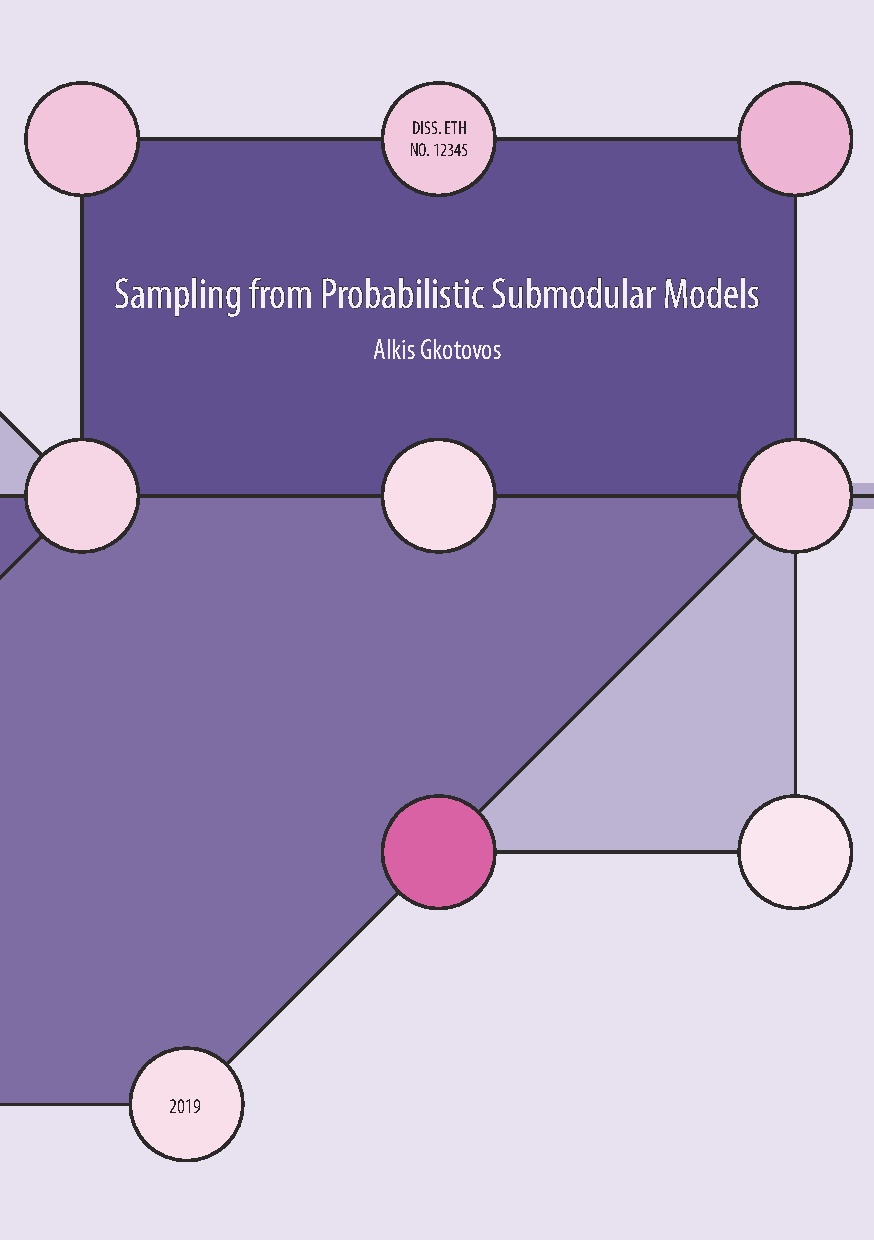
\includepdf[pages={1}]{title/outer.pdf}

\includepdf[pages={1}]{title/inner.pdf}

\cleardoublepage
\section*{Abstract}
\todo{}

\cleardoublepage
\section*{Zusammenfassung}
\todo{}

\cleardoublepage
\section*{Acknowledgements}
\todo{}
{
\hypersetup{linkcolor=black}
\tableofcontents
}

\mainmatter
\pagestyle{mainmatter}
%\renewcommand{\chaptermark}[1]{\markboth{Ch. \thechapter\ \ #1}{}}
\renewcommand{\chaptermark}[1]{\markboth{\thechapter.\ \ #1}{}}
\renewcommand{\sectionmark}[1]{\markright{\thesection\ \ #1}}

\chapter{Introduction} \label{ch:intro}
To introduce the main concepts of this thesis, we begin with a motivation application from the field of cancer genomics.
One of the major undertakings in large-scale cancer genomics research projects, such as The Cancer Genome Atlas \citep{tcga}, is obtaining and analyzing genetic data from cancer patients.
Beyond investigating the occurrence of genetic mutations one by one, it is of particular interest to discover meaningful interactions between groups of mutations.

For example, it has been observed that, depending on the type of cancer, there are groups of specific mutations that are approximately mutually exclusive, that is, most of the time no more than one mutation from a particular group occurs in the same patient \citep{yeang08}.
Biologically this is explained by the fact that so-called driver mutations, i.e., mutations that are crucial in cancer development, often occur in a limited number of biological pathways, and mutations that affect a specific pathway tend to not occur in the same patient.
Taking this in the opposite direction, discovering groups of mutually exclusive mutations may be helpful in uncovering the structure of cancer-related pathways, and identifying important groups of driver mutations.

More concretely, assume that we are given a data set of $n$ mutations and $m$ patients.
In the simplest case, the data set contains only binary information about whether or not each mutation $i \in [n]$ occurs in each patient $j \in [m]$.
Equivalently, this can be encoded using a binary matrix, as shown in \figref{fig:bamat_1}.

\begin{figure}[htb]
\centering
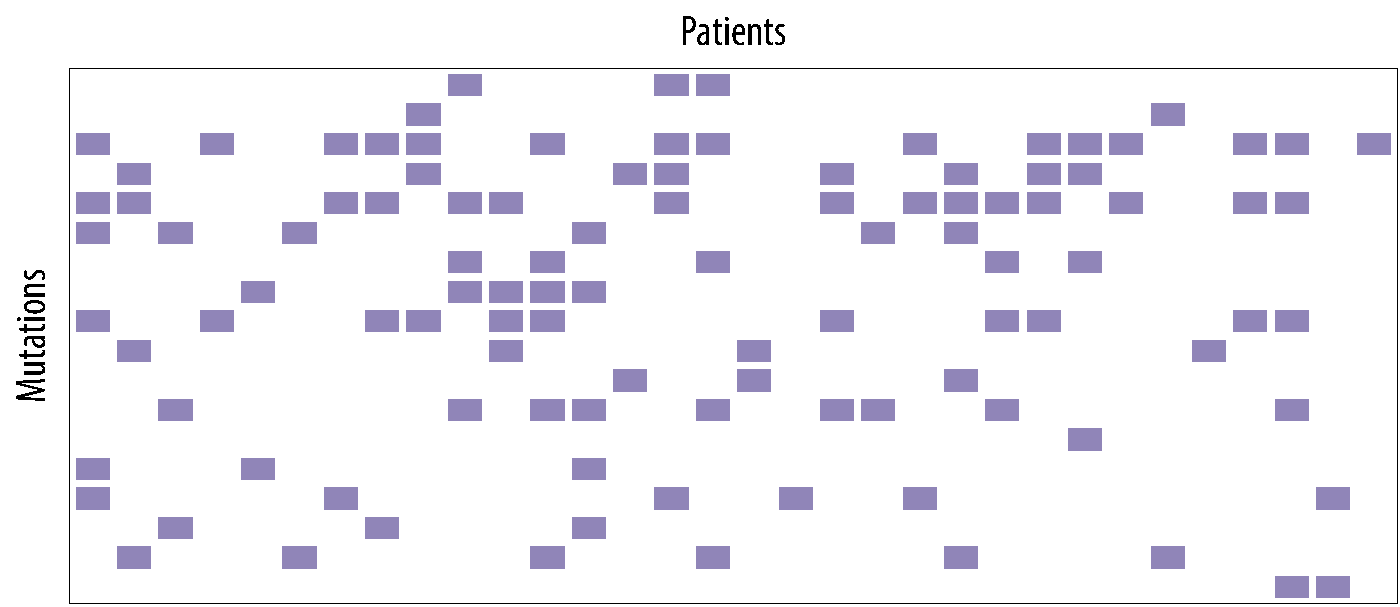
\includegraphics[width=0.9\textwidth]{figures/intro/example1.pdf}\\[1em]
\caption{An example binary mutation matrix, in which each shaded entry $(i, j)$ indicates that mutation $i$ occured in patient $j$.}
\label{fig:bamat_1}
\end{figure}

In \figref{fig:bamat_2} we show a permuted version of the previous matrix, which illustrates that the first four mutations are approximately mutually exclusive.
Searching for such groups in data sets containing hundreds or thousands of mutations is a combinatorially daunting task.
Crucially, the available data is quite limited---TCGA data sets range from a few hundred to a couple of thousand patients---, and contains significant noise introduced by the employed measurement and preprocessing procedures.

\begin{figure}[tb]
\centering
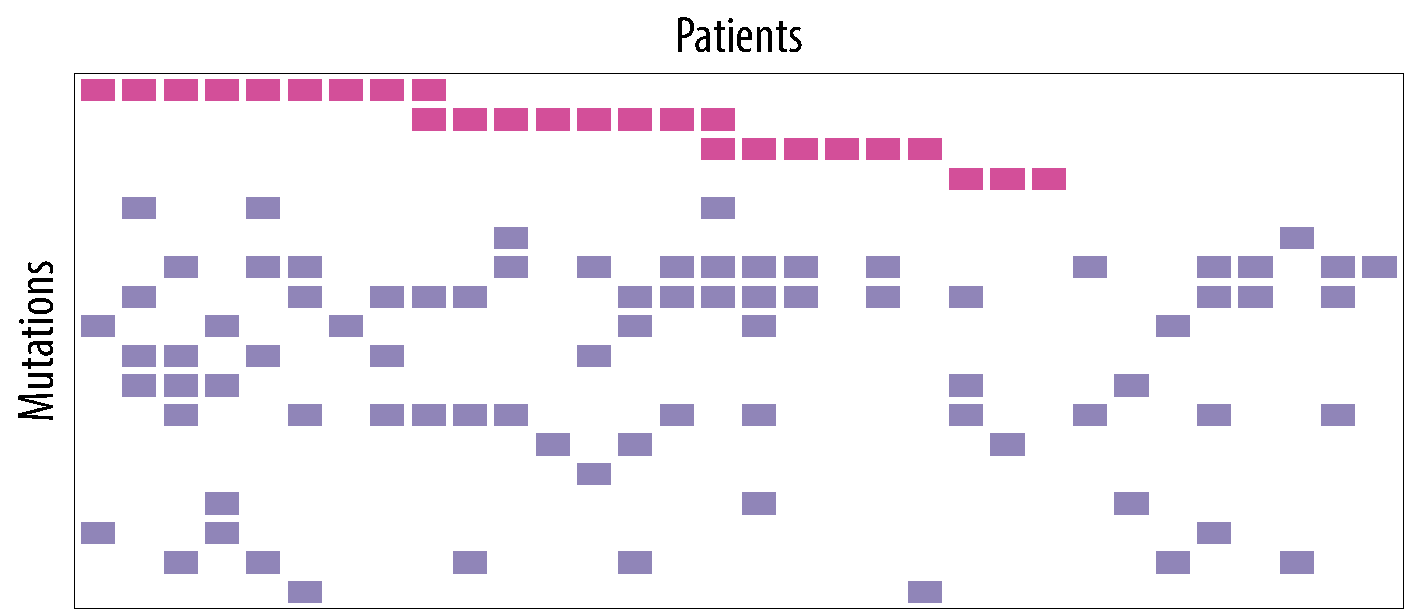
\includegraphics[width=0.9\textwidth]{figures/intro/example1_rep.pdf}\\[1em]
\caption{The binary mutation matrix of the previous figure with permuted rows and columns to illustrate the mutual exclusivity between the first four mutations.}
\label{fig:bamat_2}
\end{figure}

Many practical machine learning problems are of discrete nature, that is, like the problem described above, they consist in choosing a subset out of a set of finite elements.
Examples include sensor placement \citep{krause06}, active learning \citep{golovin11}, influence maximization \citep{kempe03}, image segmentation \citep{jegelka11}, and document summarization \citep{lin11}.
While discrete optimization methods have been successful in many of these applications, it is often advantageous to go beyond optimization, and consider discrete probabilistic models.

The probabilistic nature of such models offers a way to deal with noisy data, and provides a flexible framework to robustly answer queries pertaining to the problem at hand.
Rather than having a single optimum as the solution, we have a way to quantify our uncertainty about the most likely configurations, and make robust decisions based on computing various marginal and conditional probabilities of interest (e.g., given that element $A$ is present, what is the probability that elements $B$ and $C$ are also present).
In addition, the use of probabilistic models suggests a principled approach for learning the potentially complex interactions present in the data, namely maximizing the likelihood of the model parameters.
Finally, constraining ourselves to specific model classes allows us to incorporate prior assumptions about the problem structure, and alleviate the scarce data issue.

\section{Thesis Topic}
Past research on discrete probabilistic models has primarily focused on models defined by pairwise interactions, such as Markov random fields \cite{koller09}.
In many applications, however, it is of importance to directly capture higher-order dependencies between larger groups of variables.
For example, in our aforementioned application, being able to directly encode larger groups of mutually exclusive mutations provides a potentially sparser and easier to interpret representation, while at the same time allowing for a richer structure of interactions.

On the other hand, in the context of discrete optimization, there has been extensive research on submodular set functions.
Submodularity is a diminishing returns property that has been used to encode repulsiveness or diversity; it can, thus, be applied to model mutual exlusivity between mutations in our application.
Analogously, its counterpart, supermodularity, has been used to encode attractiveness or cooperation, and can be used to model co-occurence of mutations in our application.
Notably, there exist well-known efficient algorithms for both approximate submodular maximization, as well as submodular minimization.

Merging these two directions naturally leads us to consider \emph{probabilistic submodular models} \citep{djolonga14,gotovos15}, a class of discrete probabilistic models defined by submodular (or supermodular) functions.
More concretely, given a ground set $V = \{1,\ldots n\}$, a probabilistic submodular model is a distribution over subsets of $V$ of the form
\begin{align*}
p(S; \btheta) = \frac{1}{Z(\btheta)} \exp\left( F(S; \btheta) \right),
\end{align*}
for all $S \subseteq V$, where $F$ is a submodular or supermodular function parameterized by $\btheta$, and $Z(\btheta)$ is the normalizer of the distribution.
Distributions of this form generalize some well-studied model classes, such as Ising models, and determinantal point processes.

\paragraph{Thesis topic.} Both learning the parameters $\btheta$ from data, as well as quantifying uncertainty and making decisions with the learned distribution, boil down to the fundamental task of probabilistic inference, that is, computing marginal probabilities or the normalizer $Z$ in such distributions, a problem that is known to be computationally intractable in general.
The main topic of this thesis is to investigate the use of Markov chain Monte Carlo sampling as a means of performing approximate inference in probabilistic submodular models.

\newpage
\section{Contributions}
The primary contributions of this thesis can be summarized as follows.
\begin{itemize}[leftmargin=3.5em]
\item[\textsf{Chapter 3}] We analyze the Gibbs sampler in probabilistic submodular models, and prove sufficient theoretical conditions for polynomial-time, and fast---$\mathcal{O}(n\log n)$---mixing.
\item[\textsf{Chapter 4}] We propose a novel sampler that makes use of discrete semigradients to perform efficient global moves in the state space to avoid bottlenecks, thus leading to improved mixing over the Gibbs sampler.
\item[\textsf{Chapter 5}] We use sampling to learn probabilistic submodular models via approximate likelihood maximization, and apply this procedure to the problem of modeling interactions between genetic mutations in cancer patients.
Many of our results demonstrate considerable improvement over the state of the art.
\end{itemize}

\section{Collaborators}
The topic of sampling from probabilistic submodular models was conceived by my advisor, Prof. Andreas Krause, who has also contributed to most parts of this thesis by providing invaluable input and feedback over the years.
Parts of the theoretical analysis in \chapref{ch:gibbs} and \chapref{ch:m3} were done in collaboration with Prof. Hamed Hassani.
The work of \chapref{ch:m3} was done under the guidance of Prof. Stefanie Jegelka, who also contributed to the theoretical analysis of this chapter.
Finally, regarding the application presented in \chapref{ch:genes}, I have had fruitful discussions with Gideon Dresdner, Dr. Kjong Lehmann, and Prof. Gunnar Rätsch.
\chapter{Background} \label{ch:background}

\section{Submodularity} \label{sect:bg_submod}

Modeling notions such as coverage, representativeness, or diversity is an important challenge in many machine learning problems.
These notions are well captured by submodular set functions.
Analogously, supermodular functions capture notions of smoothness, regularity, or cooperation. 
As a result, submodularity and supermodularity have found numerous applications in machine learning problems of discrete nature, akin to concavity and convexity for continuous optimization.

\subsection{Basics}
We consider set functions $F : 2^V \to \mathbb{R}$, where $V$ is a finite ground set of size $|V| = n$.
Without loss of generality, if not otherwise stated, we will hereafter assume that $V = [n] \defeq \{1, 2, \ldots,n\}$.
Adding an element $i$ to a set $S$ results in a difference in the value of $F$ that is called marginal gain, and is defined as follows.
\begin{definition}[Marginal gain]
For any $i \in V$, and $S \subseteq V$, the marginal gain of adding $i$ to $S$ is
\begin{align*}
F(i \mid S) \defeq F(S \cup \{i\}) - F(S).
\end{align*}
\end{definition}

Intuitively, submodularity expresses a notion of diminishing returns; that is, adding an element to a larger set provides less benefit than adding it to a smaller one.
\begin{definition}[Submodularity]
$F$ is submodular if, for any $S \subseteq T \subseteq V$, and any $v \in V \setminus T$, it holds that
\begin{align*}
F(v\mid T) \leq F(v\mid S).
\end{align*}
\end{definition}
\noindent The following is an equivalent definition of submodularity that will also be useful later in the thesis.
\begin{definition}[Submodularity] \label{def:submod}
$F$ if submodular if, for any $A, B \subseteq V$, it holds that
\begin{align*}
F(A \cup B) + F(A \cap B) \leq F(A) + F(B).
\end{align*}
\end{definition}

Supermodularity is defined analogously by reversing the sign of the above inequalities.
\begin{definition}[Supermodularity] \label{def:supermod}
A function $F$ is supermodular if and only if $-F$ is submodular.
\end{definition}

If a function $m$ is both submodular and supermodular, then it is called modular.
Modular functions can be seen as the discrete analogue of linear continuous functions, and can be defined using a sum over real-numbered ``utilities''.
\begin{definition}[Modularity]
A function $m$ is called modular if it is both submodular and supermodular; it can be written as
\begin{align*}
F(S) = c + \sum_{i \in S} m_i,
\end{align*}
where $c \in \mathbb{R}$, and $m_i \in \mathbb{R}$, for all $i \in V$.
\end{definition}

A function is called monotone when adding an element can never decrease its value.
\begin{definition}[Monotonicity]
A function $F$ is monotone if, for any $i \in V$, and $S \subseteq V$, it holds that
\begin{align*}
F(i \mid S) \geq 0.
\end{align*}
\end{definition}
Furthermore, a function $F$ is called normalized if $F(\varnothing) = 0$.
In some of our results we will use the fact that we can separate the non-normalized, and non-monotone parts of any submodular function according to the following decomposition.
\begin{definition}[Submodular decomposition] \label{def:decomp}
Any submodular function $F$ can be decomposed as
\begin{align} \label{eq:decomp}
  F(S) = c + m(S) + f(S),
\end{align}
for all $S \subseteq V$, where $c \in \mathbb{R}$ is a constant, $m$ is a normalized modular function, and $f$ is a normalized monotone submodular function.
\end{definition}
An analogous decomposition using a monotone supermodular function $f$ is possible for any supermodular function $F$ as well.

\subsection{Submodular Maximization}
Perhaps the most celebrated result pertaining to submodular functions is the approximation guarantee for maximizing a monotone submodular function under a cardinality constraint.
Although the maximization problem itself is NP-hard, \cite{nemhauser78} showed that the simple greedy \algoref{alg:greedy}, which repeatedly adds the element with the maximum marginal gain, identifies a solution that is within a factor of $1 - 1/e$ of the optimal value.
\begin{theorem}[\hspace{1sp}\citealp{nemhauser78}]
For any normalized monotone submodular function $F$, the solution $S^*$ returned by \algoref{alg:greedy} satisfies
\begin{align*}
F(S^*) \geq \left(1 - \frac{1}{e}\right) \max_{S \subseteq V, |S| \leq k} F(S).
\end{align*}
\end{theorem}

\begin{algorithm}[tb]
  \setstretch{1.3}
  \DontPrintSemicolon
  \caption{\strut Greedy submodular maximization}
  \label{alg:greedy}
  \vspace{0.5em}
  \SetKwInOut{Input}{Input}
  \Input{Set function $F$, cardinality constraint $k$}
  $S^*$ $\gets$ $\varnothing$\;
  \For{$j = 1$ \KwTo $k$}{
  Select $i^*$ $\in$ $\argmax_{i \in V \setminus S^*} F(i \mid S^*)$\;
  $S^*$ $\gets$ $S^* \cup \{i^*\}$\;
  }
  \Return{$S$}\;
\end{algorithm}

Numerous extensions and generalizations of this result have been studied, including approximation guarantees for the non-monotone setting \citep{feige11,buchbinder14}; for different kinds of constraints, such as matroid \citep{lee09,calinescu11} and knapsack \citep{chekuri11}; and for the adaptive setting \citep{golovin11,gotovos15}.


\section{Discrete Probabilistic Models, Inference, and Learning}
As stated in the introduction, in the interest of venturing beyond discrete optimization, we consider discrete probabilistic models, that is, distributions over finite subsets of the ground set $V$ defined as
\begin{align*}
p(S; \btheta) = \frac{1}{Z(\btheta)} \exp\left( F(S; \btheta) \right),
\end{align*}
for all $S \subseteq V$.
The function $F$ is parameterized by a (possibly to be learned) vector $\btheta$, and $Z(\btheta)$ denotes the normalizing constant of the distribution, which is also often referred to as the partition function, and defined as
\begin{align*}
Z(\btheta) \defeq \sum_{S \subseteq V} \exp\left( F(S; \btheta) \right).
\end{align*}
An alternative and equivalent way of defining distributions of the above form is via binary random vectors $X \in \{0, 1\}^n$.
If we define $V(X) \defeq \sdef{v \in V}{X_v = 1}$, it is easy to see that the distribution $p_X(X) \propto \exp(\beta F(V(X)))$ over binary vectors is isomorphic to the above distribution over sets.
With a slight abuse of notation, we will use $F(X)$ to denote $F(V(X))$, and use $p$ to refer to both distributions.

For large parts of this thesis, we will focus on such distributions with $F$ being submodular or supermodular.
\begin{definition}[Probabilistic submodular model]
A probabilistic submodular model \citep{djolonga14,gotovos15} is a distribution of the form
\begin{align*}
p(S; \btheta) \propto \exp\left( F(S; \btheta) \right),
\end{align*}
for all $S \subseteq V$, where $F$ is a submodular or supermodular function.
\end{definition}
The resulting models of this form are also referred to as log-submodular and log-supermodular distributions respectively.
Note that the most likely configurations in these distributions directly correspond to the maximizers of the sub- or supermodular function $F$.
Some commonly used discrete models fall under these categories; for example, the standard Ising and Potts models are log-supermodular, while determinantal point processes are log-submodular.
We now present some examples models in more detail.

\begin{example}[Product distribution]
Product or log-modular distributions describe a collection of $n$ independent binary random variables.
The corresponding function $F$ is modular, that is, $F(S) = c + \sum_{i \in S} m_i$, and the partition function can be derived in closed form as
\begin{align*}
Z = \exp(c) \prod_{i \in V} \left( 1 + \exp(m_i) \right).
\end{align*}
Consequently, a log-modular distribution can be written as
\begin{align*}
  p(S) = \frac{\exp\big( \sum_{i \in S} m_i \big)}{\prod_{i \in V} \left( 1 + \exp(m_i) \right)}.
\end{align*}
Note that the constant $c$ does not appear in the distribution.
More generally, the discrete models we consider are invariant to adding a constant to $F$, since that constant gets cancelled by the partition function $Z$.
\end{example}

\begin{example}[Ising model]
In its simplest form, the (ferromagnetic) Ising model \citep{ising} is defined via an undirected graph $(V, E)$, and a set of ``attractive'' pairwise potentials
\begin{align*}
\sigma_{i,j}(S) \defeq 4\left(\llbracket\{i \in S\}\rrbracket - 0.5\right)(\llbracket\{j \in S\}\rrbracket - 0.5),
\end{align*}
for all $\{i, j\} \in E$, where we use $\llbracket \cdot \rrbracket$ to denote the Iverson bracket, which has value $1$ when the enclosed condition is true, and $0$ otherwise.
We can see that $\sigma_{i,j}$ takes value $1$ if $S$ contains both or neither of $i, j$, and value $-1$ if it contains only one of $i$ or $j$.
It follows that $\sigma_{i, j}$ is a supermodular set function.
The Ising distribution is defined as
\begin{align*}
p(S) \propto \exp\left(\sum_{\{i,j\} \in E} \sigma_{i,j}(S)\right).
\end{align*}
It is log-supermodular, since each $\sigma_{i,j}$ is supermodular, and supermodular functions are closed under addition.

We can also define the anti-ferromagnetic Ising model by a different set of ``repulsive'' pairwise potentials $\hat{\sigma}_{i,j}(S) \defeq \sigma_{i,j}(S)$.
In this case, each $\hat{\sigma}_{i,j}$ is a submodular set function, and the resulting distribution is log-submodular.

Ising models, and Potts models \citep{potts}, which generalize Ising models from binary to $k$-state variables, originate in statistical physics, but have also found numerous applications in computer vision \citep{wang13}.
\end{example}

\begin{example}[Determinantal point process]
A determinantal point process \citep{lyons03,kulesza12} is defined via a positive semidefinite matrix $L \in \mathbb{R}^{n \times n}$, and has a distribution of the form
\begin{align*}
p(S) = \frac{\det(L_S)}{\det(L + I)},
\end{align*}
where $L_S$ denotes the square submatrix indexed by set $S$, and $I$ is the $n \times n$ identity matrix.
(We only describe here the form known as an $L$-ensemble.)
Since $F(S) = \log \det(L_S)$ is a submodular function, determinantal point processes (DPPs) are log-submodular distributions.
Interestingly, as we can see from the above equation, the partition function $Z = \det(L + I)$ can be easily computed, which makes DPPs one of very few known tractable higher-order models.

DPPs also originate in statistical physics, but have been used to encourage diversity in various machine learning applications, such as image and video summarization \citep{kulesza12,gong14}.
\end{example}

\begin{example}[\flid{}]
\cite{tschiatschek16} defined the class of facility location diversity (\flid) models by means of facility location functions, that is, functions of the form
\begin{align*}
F(S) = \sum_{i \in S} u_i + \sum_{j=1}^{L} \left(\max_{i \in S} w_{ij} - \sum_{i \in S} w_{ij}\right),
\end{align*}
where $w_{ij} \geq 0$.
This is a submodular set function, therefore the resulting distribution $p(S) \propto \exp(F(S))$ is log-submodular.

The above function $F$ is parameterized by a utility vector $\bu \in \mathbb{R}^n$, and a diversity matrix $\bw \in \mathbb{R}^{n\times L}$.
Increasing the utility $u_i$ of an element $i \in S$ intuitively increases the probability of all sets containing that element, therefore also increases its marginal probability.
The diversity matrix $\bw$ can be thought of as consisting of $L$ dimensions (columns).
Elements of the ground set that have large value in the same column $j$ will tend to appear together less frequently, since the term $\max_{i \in S} w_{ij} - \sum_{i \in S} w_{ij}$ will be negative for sets $S$ that contain combinations of such items.

\todo{Show 3-element example figure.}
\end{example}

\begin{example}[\fldc{}]
\citep{djolonga16mixed}
\begin{align*}
F(S) = \sum_{i \in S} u_i + \sum_{j=1}^{L} \left(\max_{i \in S} w_{ij} - \sum_{i \in S} w_{ij}\right) - \sum_{j=1}^{L} \left(\max_{i \in S} v_{ij} - \sum_{i \in S} v_{ij}\right).
\end{align*}
\end{example}

Note that, both the facility location model and the Ising model use decomposable functions, that is, functions that can be written as a sum of simpler submodular (resp. supermodular) functions $F_{\ell}$:
\begin{align} \label{eq:fdec}
F(S) = \sum_{\ell \in [L]} F_{\ell}(S).
\end{align}


\subsection{Inference}

Recently, \citet{djolonga14} considered a more general treatment of such models, and proposed a variational approach for performing approximate probabilistic inference for them.

\todo{Exponential family}

\todo{Contrastive divergence}

Iyer and Bilmes \citep{iyer15} recently considered a different class of probabilistic models, called submodular point processes, which are also defined through submodular functions, and have the form $p(S) \propto F(S)$.
They showed that inference in SPPs is, in general, also a hard problem, and provided approximations and closed-form solutions for some subclasses.

\todo{Add Chengtao constrained etc. paper}
\todo{Add DPP -- Rayleigh papers}

\section{Sampling and Mixing Times}

\paragraph{Gibbs sampler.}
One of the most commonly used chains is the (single-site) Gibbs sampler, which adds or removes a single element %of the ground set
at a time.
It first selects uniformly at random an element $v \in V$; subsequently, it adds or removes $v$ to the current state $X_t$ according to the probability of the resulting state.
We denote by $P : \Omega \times \Omega \to \mathbb{R}$ the transition matrix of a Markov chain, that is, for all $S, R \in \Omega$, $P(S, R) \defeq \P\left[ X_{t+1} = R \mid X_t = S \right]$.
Then, if we define
\begin{align*}
p_{S \rightarrow R} = \displaystyle\frac{\exp(F(R))}{\exp(F(R)) + \exp(F(S))},
\end{align*}
and denote by $S \sim R$ states that differ by exactly one element (i.e., $\big||R| - |S|\big| = 1$),
the transition matrix $\Pg$ of the Gibbs sampler is
\begin{align*}
  \Pg(S, R) = 
  \threepartdefo{\displaystyle\frac{1}{n}p_{S \rightarrow R}}{R \sim S}{1 - \displaystyle\sum_{T \sim S} \displaystyle\frac{1}{n}p_{S \rightarrow T}}{R = S}{0}.
\end{align*}

\paragraph{Approximating the log-partition function.}
There are two straightforward methods for estimating the log-partition function using sampling.
The first one, importance sampling (IS) \citep{ais}, assumes that we have a normalized distribution $\pi$ from which we draw $M$ samples $\{x\}$

The second, reverse important sampling (RIS) \citep{ris},

\paragraph{Mixing times.}
Approximating quantities of interest using MCMC methods is based on using time averages to estimate expectations over the desired distribution.
In particular, we estimate the expected value of function $f : \ss \to \mathbb{R}$ by $\E_p[f(X)] \approx (1/T)\sum_{r=1}^{T} f(X_{s + r})$.
For example, to estimate the marginal $p(v \in S)$, for some $v \in V$, we would define $f(x) = \mathds{1}_{\{x_v = 1\}}$, for all $x \in \ss$.
The choice of burn-in time $s$ and number of samples $T$ in the above expression presents a tradeoff between computational efficiency and approximation accuracy.
It turns out that the effect of both $s$ and $T$ is largely dependent on a fundamental quantity of the chain called \emph{mixing time} \cite{levin08}.

The mixing time of a chain quantifies the number of iterations $t$ required for the distribution of $X_t$ to be close to the stationary distribution $\pi$.
More formally, it is defined as $\tme \defeq \min \sdef{t}{d(t) \leq \epsilon}$, where $d(t)$ denotes the worst-case (over the starting state $X_0$ of the chain) total variation distance between the distribution of $X_t$ and $\pi$.
Establishing upper bounds on the mixing time of our Gibbs sampler is, therefore, sufficient to guarantee efficient approximate marginal inference (e.g., see Theorem 12.19 of \citet{levin08}).
\chapter{Gibbs Sampling in Prob. Submodular Models} \label{ch:gibbs}

\emph{The majority of the content of this chapter has already been published in conference proceedings \citep{gotovos15}.}

\section{Introduction}
In this chapter, we consider one of the simplest and most commonly used sampling procedures, namely the (single-site) Gibbs sampler, which is also known as the Glauber chain.
While there has been extensive work on the properties of the Gibbs sampler on low-order models, for example, Ising models \citep[Ch. 15]{levin08book}, not much is known about its behavior on higher-order models, except that, in general, we cannot hope for sub-exponential mixing times \citep{jerrum93}.
In fact, we show that even for probabilistic submodular models defined by monotone submodular functions, there are simple model families with exponential lower bounds on mixing time.

Our goal is to establish theoretical conditions that guarantee rapid mixing of the Gibbs sampler in probabilistic submodular models, and at the same time, investigate in what way the properties of sub- and supermodularity affect the resulting conditions.


\section{Problem Setup} \label{sect:setup}
In this chapter, we focus on distributions of the form
\begin{align}\label{eq:gibbs_pdef}
p(S) = \frac{\exp(\beta F(S))}{Z},
\end{align}
for all $S \subseteq V$, where $F$ is submodular or supermodular.
We currently assume that $F$ is already learned or given, and omit the parameter vector $\btheta$ from the notation.
Furthermore, we have introduced a scaling parameter $\beta \geq 0$, which is referred to as inverse temperature, and will be useful for our subsequent theoretical analysis.
Intuitively, $\beta$ controls the concentration of $p$ around the high-value sets of $F$.
When $\beta = 0$, $p$ is the uniform distribution over $2^V$; when $\beta \to \infty$, the mass of $p$ fully concentrates around the maximizers of $F$.

\paragraph{Marginal inference.}
Our goal is to perform marginal inference for the distributions described above.
Concretely, for some fixed $A \subseteq B \subseteq V$, we would like to compute the probability of sets $S$ that contain all elements of $A$, but no elements outside of $B$, that is, $p(A \subseteq S \subseteq B)$.
More generally, we are interested in computing conditional probabilities of the form $p(A \subseteq S \subseteq B \mid C \subseteq S \subseteq D)$.
This computation can be reduced to computing unconditional marginals as follows.
For any $C \subseteq V$, define the contraction of $F$ on $C$, $F_C : 2^{V \setminus C} \to \mathbb{R}$, by $F_C(S) = F(S \cup C) - F(S)$, for all $S \subseteq V \setminus C$.
Also, for any $D \subseteq V$, define the restriction of $F$ to $D$, $F^D : 2^D \to \mathbb{R}$, by $F^D(S) = F(S)$, for all $S \subseteq D$.
If $F$ is submodular, then its contractions and restrictions are also submodular, and, thus, $(F_C)^D$ is submodular.
Finally, it is easy to see that $p(S \mid C \subseteq S \subseteq D) \propto \exp(\beta (F_C)^D(S))$.
In our experiments, we consider computing marginals of the form $p(i \in S \mid C \subseteq S \subseteq D)$, for some $i \in V$, which correspond to $A = \{i\}$, and $B = V$.

\section{Hardness of Inference}
Performing exact inference in probabilistic submodular models is, in general, computationally infeasible.
Only for very few exceptions, such as determinantal point processes, is exact inference possible in polynomial time \citep{kulesza12}.
As we mentioned before, even approximating the partition function of general Ising models---a subclass of PSMs---is a hard problem; in particular, there is no FPRAS for this problem, unless RP = NP \citep{jerrum93}.
This implies that the mixing time of any Markov chain with such a stationary distribution will, in general, be exponential in $n$.

\subsection{Example: Log-submodular Grid}
To further highlight the hardness of inference in the general models we consider, we show that even for distributions defined through a seemingly benign subclass of submodular functions, mixing times can be exponential in $n$.
We say that a set function $F : 2^V \to \mathbb{R}$ is monotone, if $F(i \mid S) \geq 0$, for all $i \in V$, and all $S \subseteq V$.
Intuitively, adding elements to our set always leads to higher values.

For the purposes of the following proposition, we will use a Metropolis chain (see \sectref{sect:sampling}), rather than a Gibbs chain, to simplify the exposition.
While the two chains are not identical, they share the same principle of making local moves by considering ratios of probabilities of neighboring states.
\begin{prop}
There is a family of monotone submodular functions $(F_n)_n$, such that, for the corresponding log-submodular family of distributions $(p_n)_n$ defined as in \eqref{eq:gibbs_pdef}, the Metropolis chain has mixing time
\begin{align*}
  \tm  = \Omega(2^{n/2}),
\end{align*}
for any value of $\beta$.
\end{prop}

\begin{proof}
The functions used to prove the above lemma are based on the following construction.
For any even $n \geq 2$, let $V_n = \{1,\ldots,n\}$, $R_n = \{1,\ldots,n/2\}$, and $C_n = \{n/2+1,\ldots,n\}$.
To define function $F_n : 2^{V_n} \to \mathbb{R}$, we conceptually use a $n/2 \times n/2$ square grid, whose rows are indexed by $R$ and columns by $C$.
Each cell $(i, j)$ of the grid is considered to be covered, if either row $i \in R$ or column $j \in C$ is selected.
Formally, we define $F_n$ by
\begin{align*}
  F_n(S) = \frac{4}{n^2}\big\vert \sdef{(i, j) \in R \times C}{i \in S \lor j \in S}\big\vert,
\end{align*}
for any $S \subseteq V_n$, which results in $F_n(V_n) = 1$.
\figref{fig:submod_grid} shows an example of such a grid construction.

\begin{figure}[htb]
  \centering
  \begin{tikzpicture}[
	%baseline,
	scale=0.9
	]
    
	\fill[col1] (0,3) rectangle (4,4);
	\fill[col1] (0,1) rectangle (4,2);
	\fill[col1] (2,0) rectangle (3,4);
	\draw[step=1cm,black!70!white,line width=1.5pt] (0,0) grid (4,4);
	
	\node at (-0.3,3.5) {\sffamily 1};
	\node at (-0.3,2.5) {\sffamily 2};
	\node at (-0.3,1.5) {\sffamily 3};
	\node at (-0.3,0.5) {\sffamily 4};
	\node at (0.5,4.3) {\sffamily 5};
	\node at (1.5,4.3) {\sffamily 6};
	\node at (2.5,4.3) {\sffamily 7};
	\node at (3.5,4.3) {\sffamily 8};
\end{tikzpicture}\\[1em]
  \caption{Example grid for $n = 8$ with the cells corresponding to $F_8(\{1,3,7\}) = 10/16$ shown shaded.}
  \label{fig:submod_grid}
\end{figure}

\newcommand{\hrn}{\mathcal{R}_n}
\newcommand{\hcn}{\mathcal{C}_n}
\newcommand{\hkn}{\mathcal{K}_n}
\newcommand{\htn}{\mathcal{T}_n}

Furthermore, if we define $\hrn = \{S \subseteq V \mid R \subseteq S\}$, $\hcn = \{S \mid C \subseteq S \subseteq V\}$, and $\hkn = 2^V \setminus (\hrn \cup \hcn)$, then the following properties hold.
\begin{align}
  &|\hrn| = |\hcn| = 2^{n/2} \label{eq:prop1} \\
  &\hrn \cap \hcn = \{V\} \label{eq:prop2} \\
  &\forall S \in \hrn\cup\hcn,\ f(S) = 1 \label{eq:prop3} \\
  &\forall S \in \hkn,\ f(S) \leq 1 - 4/n^2 \label{eq:prop4}.
\end{align}
Assume a Metropolis chain with transition matrix $P$, and stationary distribution $p_n(S) \propto \exp(\beta F_n(S))$.
To prove a lower bound on the mixing time of this chain, we are going to upper bound the bottleneck ratio \citep[Ch. 7]{levin08} of set $\htn = \hrn \setminus \{V\}$, defined as
\begin{align*}
  \Phi(\htn) = \frac{Q(\htn, \htn^c)}{\pi(\htn)} = \frac{Q(\htn, \hcn) + Q(\htn, \hkn)}{\pi(\htn)},
\end{align*}
where $\htn^c = 2^V \setminus \htn$ is the complement of $\htn$. We now compute or bound each of the terms $\pi(\htn)$, $Q(\htn, \hcn)$, and $Q(\htn, \hkn)$.

\paragraph{Computing $\pi(\htn)$.}
\begin{align*}
  \pi(\htn) &= |\htn| \frac{e^{\beta}}{Z} \tag*{by \eqref{eq:prop3}} \\
         &= (2^{n/2} - 1) \frac{e^{\beta}}{Z}. \tag*{by \eqref{eq:prop1}}
\end{align*}
Note that, by an analogous derivation, we get $\pi(\hcn \setminus \{V\}) = \pi(\htn)$ and, by \eqref{eq:prop2},
\begin{align*}
  &\pi(\htn) + \pi(\hcn \setminus \{V\}) < 1 \\
  \Rightarrow\ \ &\pi(\htn) < 0.5.
\end{align*}
  
\paragraph{Computing $Q(\htn, \hcn)$.}
\begin{align*}
  Q(\htn, \hcn) &= \sum_{x \in \htn} Q(x, \hcn) \\
                &= \sum_{x \in \htn} Q(x, \{V\}) \tag*{by \eqref{eq:prop2}} \\
                &= \sum_{x \in \htn} \frac{1}{2n} \frac{e^{\beta}}{Z} \tag*{by \eqref{eq:prop3}} \\
                &= n \frac{1}{2n} \frac{e^{\beta}}{Z} = \frac{e^{\beta}}{2Z}.
\end{align*}
    
\paragraph{Bounding $Q(\htn, \hkn)$.}
\begin{align*}
  Q(\htn, \hkn) &= \sum_{x \in \htn} Q(x, \hkn) \\
                &\leq \sum_{x \in \htn} \frac{1}{2n} \frac{e^{\beta - 4\beta/n^2}}{Z} \tag*{by \eqref{eq:prop4}} \\
                &= \frac{2^{n/2} - 1}{2n} \frac{e^{\beta - 4\beta/n^2}}{Z}. \tag*{by \eqref{eq:prop1}}
\end{align*}

\paragraph{Bounding $\Phi(\htn)$.}
\begin{align*}
  \Phi(\htn) &\leq \frac{1}{2^{n/2} - 1}\left(\frac{1}{2} + \frac{(2^{n/2} - 1) e^{-4\beta/n^2}}{2n}\right)\\
          &= \frac{1}{2(2^{n/2} - 1)} + \frac{e^{-4\beta/n^2}}{2n}.
\end{align*}
Using Theorem 7.3 \citep{levin08book}, it follows that
\begin{align*}
  \tm(1/4) \geq \frac{1}{4\Phi(\htn)} = \Omega(2^{n/2}).
\end{align*}

\end{proof}

\section{Polynomial-time Mixing} \label{sect:poly}
Our first result provides conditions that guarantee polynomial mixing times in the size of the ground set $n$.
As we will see, the conditions depend crucially on the following quantity, which is defined for any set function $F : 2^V \to \mathbb{R}$:
\begin{align*}
  \zf \defeq \max_{A, B \subseteq V} \left|F(A) + F(B) - F(A \cup B) - F(A \cap B) \right|.
\end{align*}
Intuitively, $\zf$ quantifies a notion of distance to modularity.
For submodular and supermodular functions, $\zf$ represents the worst-case amount by which $F$ violates the submodular inequality, and $\zf = 0$ if $F$ is modular (cf. \sectref{sect:bg_submod}).

It is also important to note that, for submodular and supermodular functions, $\zf$ depends only on the monotone part of $F$; if we decompose $F$ according to \defref{def:decomp}, then it is easy to see that $\zf = \zeta_f$.
A trivial upper bound on $\zf$, therefore, is $\zf \leq f(V)$.
Another quantity that has been used in the past to quantify the deviation of a submodular function from modularity is the curvature \citep{conforti84}, defined as $\kappa_F \defeq 1 - \min_{i \in V} \left(F(i\mid V\setminus\{i\}) / F(i)\right)$.
Although of similar intuitive meaning, the multiplicative nature of its definition makes it significantly different from $\zf$, which is defined additively.

\subsection{Examples}
\paragraph{Concave over modular.}
As an example of a function class with $\zf$ independent of $n$, assume a ground set $V = \bigcup_{\ell = 1}^L V_{\ell}$, and consider functions of the form
\begin{align*}
F(S) = \sum_{\ell = 1}^L \phi(|S \cap V_{\ell}|),
\end{align*}
where $\phi : \mathbb{R} \to \mathbb{R}$ is a bounded concave function, e.g, $\phi(x) = \min\{\phi_{\max}, x\}$.
Functions of this form are submodular, and have been used in applications such as document summarization to encourage diversity \citep{lin11}.
It is easy to see that $\zf \leq L\phi_{\max}$, which shows that $\zf$ is independent of $n$.

\paragraph{\flid{}.}
For the \flid{} model (see \exampleref{ex:flid}), we have $f(S) = \sum_{j=1}^L \max_{i \in S} w_{ij}$, therefore we get $\zf \leq f(V) = \sum_{j=1}^L w_j^{\mathrm{max}}$, where $w_j^{\mathrm{max}} = \max_{i \in V} w_{ij}$.
Since the values of $\bw$ depend primarily on the number of repulsive groups, rather than the size of the ground set, we expect $\zf$ to grow much slower than $n$ in most practical applications.

\paragraph{\fldc{}.}
For the \fldc{} model (see \exampleref{ex:fldc}), although $F$ is neither submodular nor supermodular in general, we can still write it as
\begin{align*}
F(S) = m(S) + g(S) + h(S),
\end{align*}
where $m$ is a modular function, $g(S) \defeq \sum_{j=1}^L \max_{i \in S} w_{ij}$ is submodular, and $h(S) \defeq -\sum_{j=1}^K \max_{i \in S} v_{ij}$ is supermodular.
Using the triangle inequality in the definition of $\zf$, we get that $\zf \leq g(V) + h(V) = \sum_{j=1}^L w_j^{\mathrm{max}} + \sum_{j=1}^K v_j^{\mathrm{max}}$, where $w_j^{\mathrm{max}} = \max_{i \in V} w_{ij}$, and $v_j^{\mathrm{max}} = \max_{i \in V} v_{ij}$.

\subsection{Mixing Time Bound}
\noindent The following theorem establishes a bound on the mixing time of the Gibbs sampler run on models of the form \eqref{eq:gibbs_pdef}.
The bound is exponential in $\zf$, but polynomial in $n$.
\begin{theorem} \label{thm:poly}
  For any function $F : 2^V \to \mathbb{R}$, the mixing time of the Gibbs sampler is bounded by
  \begin{align*}
    \tme \leq 2n^2 \exp(2 \beta \zf) \log\left(\frac{1}{\epsilon p_{\min}}\right),
  \end{align*}
  where $p_{\min} \defeq \displaystyle\min_{S \in \ss}p(S)$.
  If $F$ is submodular or supermodular, then the bound is improved to
  \begin{align*}
    \tme \leq 2n^2 \exp(\beta \zeta_f) \log\left(\frac{1}{\epsilon p_{\min}}\right).
  \end{align*}
\end{theorem}
Note that, since the factor of two that constitutes the difference between the two statements of the theorem lies in the exponent, it can have a significant impact on the above bounds.
The dependence on $p_{\min}$ is related to the (worst-case) starting state of the chain, and can be eliminated if we have a way to guarantee a high-probability starting state.
If $F$ is submodular or supermodular, this is usually straightforward to accomplish by using one of the standard constant-factor optimization algorithms \citep{nemhauser78,fujishige05} as a preliminary step.
More generally, if $F$ is bounded by $0 \leq F(S) \leq F_{\max}$, for all $S \subseteq V$, then $\log (1/p_{\min}) = \mathcal{O}(n \beta F_{\max})$.

\paragraph{Canonical paths}
Our proof of \theoremref{thm:poly} is based on the method of \emph{canonical paths} \citep{jerrum03,sinclair92,jerrum89,diaconis91}.
The high-level idea of this method is to view the state space as a graph, and try to construct a path between each pair of states, which carries a certain amount of flow specified by the stationary distribution under consideration.
Depending on the choice of these paths and the resulting load on the edges of the graph we can derive bounds on the mixing time of the Markov chain.

More concretely, let us assume that for some set function $F$ and corresponding distribution $p$ as in \eqref{eq:gibbs_pdef}, we construct the Gibbs chain on state space $\ss = 2^V$ with transition matrix $P$.
We can view the state space as a directed graph that has vertex set $\ss$, and for any $A, B \in \ss$, contains edge $(S, S')$ if and only if $S \sim S'$, that is, if and only if $S$ and $S'$ differ by exactly one element.
Now, for any pair of states $A, B \in \ss$, we define a \emph{canonical path}
\begin{align*}
\gamma_{AB} \defeq (A = S_0, S_1, \ldots, S_{\ell} = B),
\end{align*}
such that all $(S_i, S_{i+1})$ are edges in the above graph.
We denote the length of path $\gamma_{AB}$ by $|\gamma_{AB}|$, and define $Q(S, S') \defeq p(S) P(S, S')$.
We also denote the set of all pairs of states whose canonical path goes through $(S, S')$ by
\begin{align*}
\mathcal{C}_{SS'} \defeq \sdef{(A, B) \in \ss \times \ss}{(S, S') \in \gamma_{AB}}.
\end{align*}
The following quantity, referred to as the \emph{congestion} of an edge, uses a collection of canonical paths to quantify to what amount that edge is overloaded:
\begin{align} \label{eq:cong}
  \rho(S, S') \defeq \frac{1}{Q(S, S')} \sum_{(A, B) \in \mathcal{C}_{SS'}} p(A) p(B) |\gamma_{AB}|.
\end{align}
The denominator $Q(S, S')$ quantifies the capacity of edge $(S, S')$, while the sum represents the total flow through that edge according to the choice of canonical paths.
The congestion of the whole graph is then defined as $\rho \defeq \max_{S \sim S'}\rho(S, S')$.
Low congestion implies that there are no bottlenecks in the state space, and the chain can move around fast, which results in rapid mixing.
The following theorem makes this statement more concrete.

\begin{theorem}[\hspace{1sp}\citealp{sinclair92,jerrum03}] \label{thm:cpath}
  For any collection of canonical paths with congestion $\rho$, the mixing time of the chain is bounded by
  \begin{align*}
  	\tme \leq \rho \log\left(\frac{1}{\epsilon p_{\mathrm{min}}}\right),
  \end{align*}
where $p_{\mathrm{min}} \defeq \displaystyle\min_{S \in \ss}p(S)$.
\end{theorem}

\renewcommand{\subflen}{0.48\textwidth}
\begin{figure}[tbp]
  %\captionsetup[subfigure]{oneside,margin={2em,0em}}
  \begin{subfigure}[b]{\subflen}
    \centering
    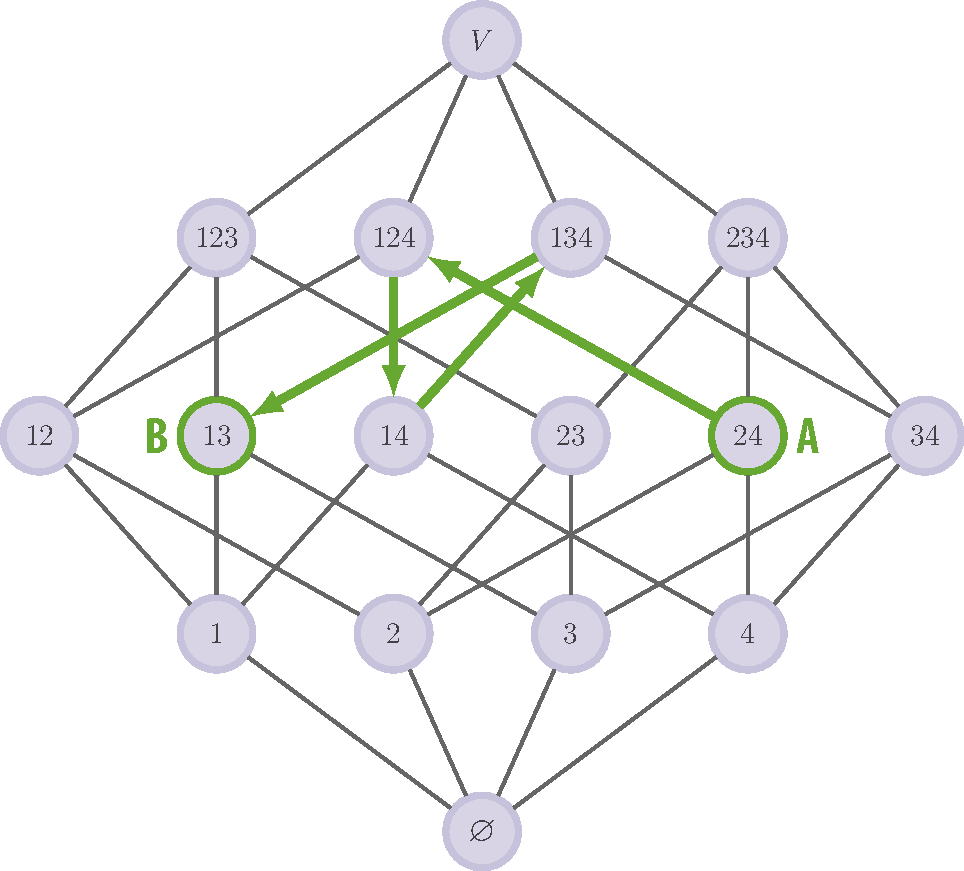
\includegraphics[width=\textwidth]{figures/gibbs/cp_easy_path_4.pdf}
    \caption{Canonical path}
    \label{fig:cong1}
  \end{subfigure}\hspace{1em}
  \begin{subfigure}[b]{\subflen}
    \centering
    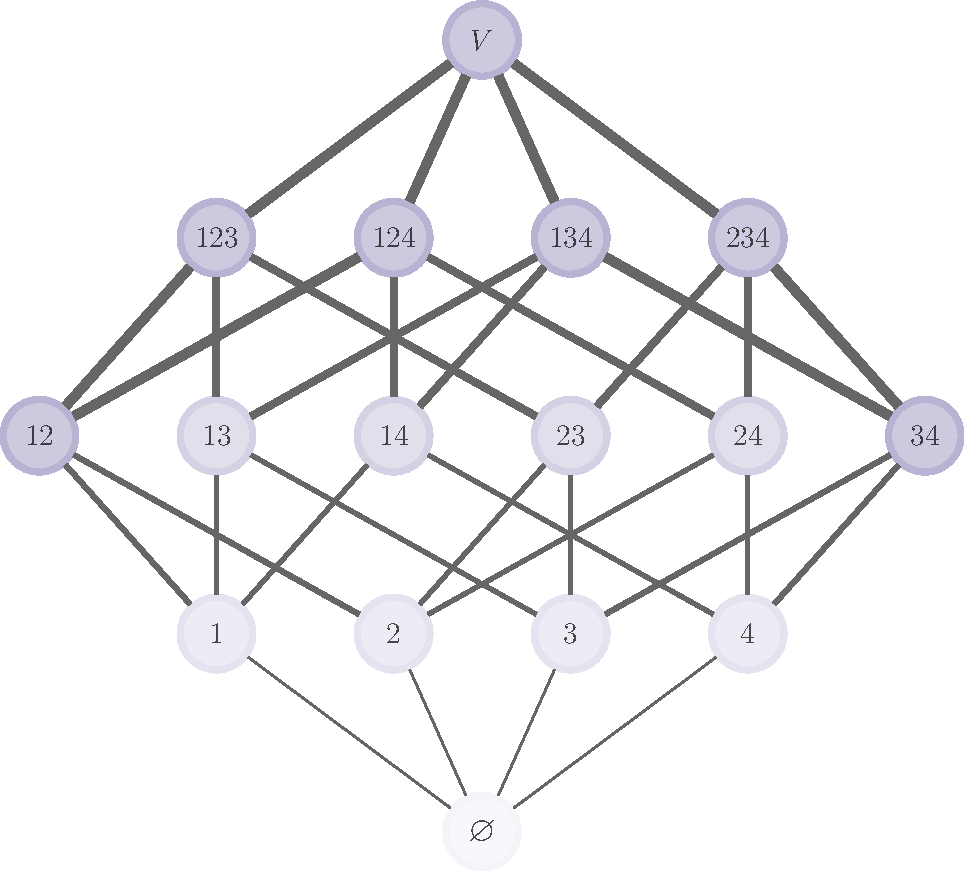
\includegraphics[width=\textwidth]{figures/gibbs/cp_easy.pdf}
    \caption{Capacities}
    \label{fig:cong2}
  \end{subfigure}\\[2em]
  \begin{subfigure}[b]{\subflen}
    \centering
    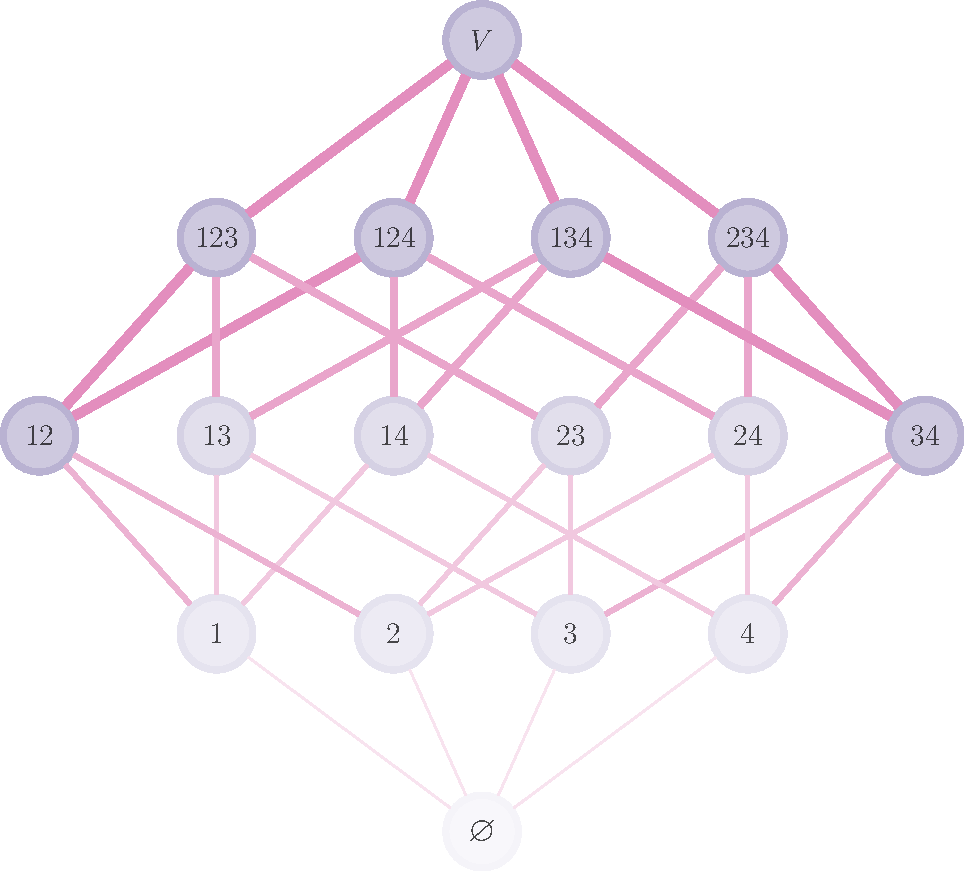
\includegraphics[width=\textwidth]{figures/gibbs/cp_easy_cong.pdf}
    \caption{Low congestion}
    \label{fig:cong3}
  \end{subfigure}\hspace{1em}
  \begin{subfigure}[b]{\subflen}
    \centering
    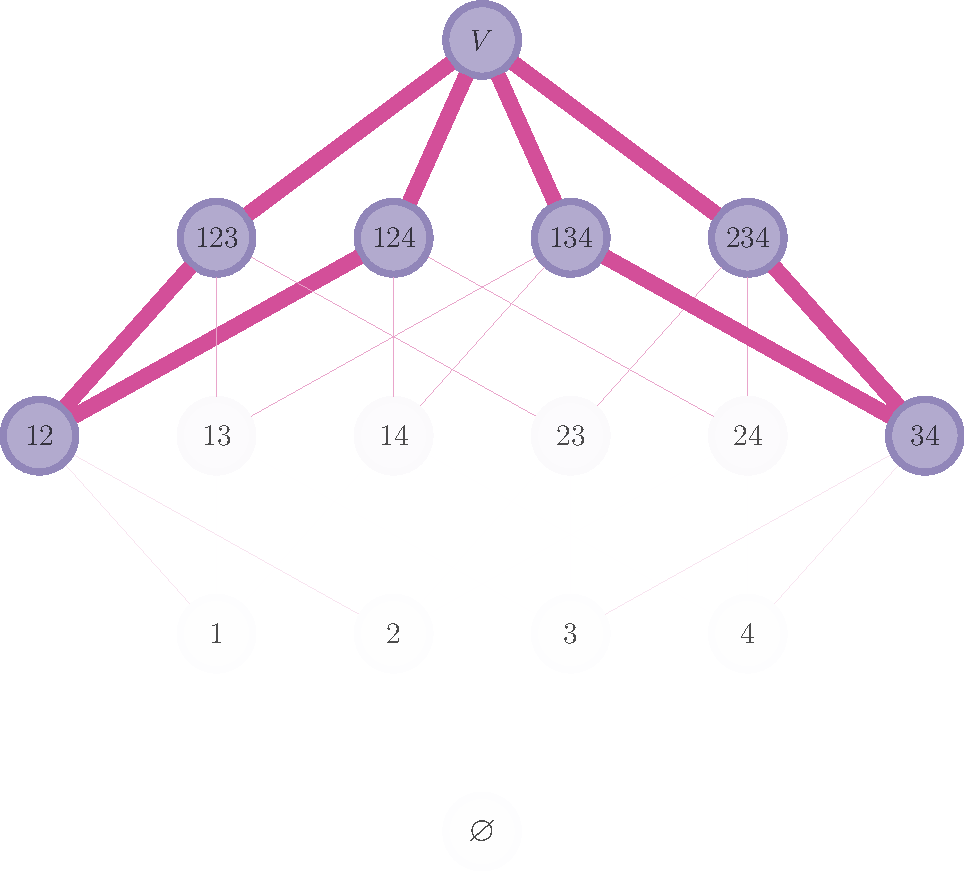
\includegraphics[width=\textwidth]{figures/gibbs/cp_hard_cong.pdf}
    \caption{High congestion}
    \label{fig:cong4}
  \end{subfigure}\\
  \caption{(a) The state space for ground set $V = \{1, 2, 3, 4\}$, and an illustration of a canonical path from $A = \{2, 4\}$ to $B = \{1, 3\}$.
  (b) For an example distribution $p$, the width of each edge denotes the corresponding capacity $Q(S, S')$.
  (c) The color of each edge denotes the corresponding congestion $\rho(S, S')$; darker edges indicate higher congestion.
  (d) Similar to (c), but for a different distribution that has almost all of its mass concentrated on seven states.
  It can been seen that it has notably higher congestion $\rho$, and contains a significant bottleneck at $S = \{V\}$.
  }
  \label{fig:cong}
\end{figure}

\subsection{Proof of \theoremref{thm:poly}}
To apply \theoremref{thm:cpath} to our class of distributions, we need to construct a set of canonical paths in the corresponding state space $2^V$, and upper bound the resulting congestion.
First, note that, to transition from state $A \in \ss$ to state $B \in \ss$, in our case, it is enough to remove the elements of $A \setminus B$ and add the elements of $B \setminus A$.
Each removal and addition corresponds to an edge in the state space graph, and the order of these operations identify a canonical path in this graph that connects $A$ to $B$.
For our analysis, we assume a fixed order on $V$ (e.g., the natural order of the elements themselves), and perform the operations according to this order.
\figref{fig:cong1} shows an example of such a canonical path for a small state space, and \figsref{fig:cong2}--\ref{fig:cong4} illustrate the capacities $Q(S, S')$, and congestions $\rho(S, S')$ for two example distributions.

Having defined the set of canonical paths, we proceed to bounding the congestion $\rho(S, S')$ for any edge $(S, S')$.
The main difficulty in bounding $\rho(S, S')$ is due to the sum in \eqref{eq:cong} over all pairs in $\mathcal{C}_{SS'}$.
To simplify this sum, we construct for each edge $(S, S')$ an injective map $\ess : \mathcal{C}_{SS'} \to \ss$; this is a combinatorial encoding technique that has been previously used in similar proofs to ours \citep{jerrum03}.
The following lemma details this construction, where for sets $A, B$, we denote $A \oplus B \defeq (A \setminus B)\cup(B \setminus A)$.

\begin{lemma} \label{lem:inj}
Define the maps $\ess : \mathcal{C}_{SS'} \to \ss$, for each pair $(S, S') \in \ss \times \ss$ with $S \sim S'$, as follows:
\begin{align*}
  \ess(A, B) = \twopartdefo{A \oplus B \oplus S}{F(S') \geq F(S)}{A \oplus B \oplus S'}.
\end{align*}
Then, each map $\ess$ is injective.
\end{lemma}

\begin{proof}
  Assume that $F(S') \geq F(S)$, and $S' = S \cup \{r\}$, for some $r \in V$.
  Assume that we are given $C \defeq A \oplus B \oplus S$, and we want to recover $A$ and $B$.
  We will denote by $\prec$ the natural ordering of the ground set $V$.
  First, we define
  \begin{align*}
    K^- &\defeq \sdef{i \in C \oplus S}{i \prec r}\\
    K^+ &\defeq \sdef{i \in C \oplus S}{i \succ r}.
  \end{align*}
  Then, we can recover $A$ and $V$ as follows:
  \begin{align*}
    A &= S \oplus K^-\\
    B &= S' \oplus K^+.
  \end{align*}
  The case $S' = S \setminus \{r\}$, as well as the two cases for $F(S') < F(S)$ are completely analogous.
  Note that the distinction based on the value of the function has no effect on the proof here, but is technically needed for the next lemma.
  The only thing that changes between the cases is whether the element $r$ that gets added or removed in the transition $(S, S')$ belongs to $A$ or $B$, which is always straightforward to determine from the type of the transition (for additions it belongs to $B$, and for removals to $A$).
\end{proof}
\noindent We then prove the following key lemma about the maps constructed above.
\begin{lemma} \label{lem:poly_full}
  For any $S \sim S'$, and any $A, B \in \ss$, it holds that
  \begin{align*}
    p(A)p(B) \leq 2n\exp(2 \beta \zf)Q(S, S')p(\ess(A, B)).
  \end{align*}
  
  If $F$ is submodular or supermodular, then the bound is improved to
  \begin{align*}
  	p(A)p(B) \leq 2n\exp(\beta \zeta_f)Q(S, S')p(\ess(A, B)).
  \end{align*}
\end{lemma}
\begin{proof}
  We will consider the case $S' = S \cup \{r\}$, for some $r \in V$, with $F(S') \geq F(S)$.
  Again, the other three cases are completely analogous by using $\ess$ as defined in \lemmaref{lem:inj}.
  
  We first compute
  \begin{align*}
    Q(S, S') &= p(S)P(S, S')\\
             &= \frac{1}{n}\frac{p(S)p(S')}{p(S) + p(S')} \tag*{by definition of the Gibbs sampler}\\
             &= \frac{1}{nZ}\frac{\exp(\beta F(S)) \exp(\beta F(S'))}{\exp(\beta F(S)) + \exp(\beta F(S'))} \tag*{by definition of our models}\\
             &\geq \frac{1}{nZ}\frac{\exp(\beta F(S)) \exp(\beta F(S'))}{2\exp(\beta F(S'))} \tag*{by $F(S') \geq F(S)$}\\
             &= \frac{\exp(\beta F(S))}{2nZ}.
  \end{align*}
  As a result, we get
  \begin{align} \label{eq:ppq}
    \frac{p(A)p(B)}{Q(S, S')} \leq \frac{2n}{Z}\exp(\beta (F(A) + F(B) - F(S))).
  \end{align}
  Let us denote
  \begin{align*}
    \zf(A, B) \defeq F(A) + F(B) - F(A \cup B) - F(A \cap B),
  \end{align*}
  for any $A, B \subseteq V$, so that $\zf = \max_{A, B \subseteq V}|\zf(A, B)|$.
  Then, if we denote
  \begin{align*}
    C \defeq \ess(A, B) = A \oplus B \oplus S,
  \end{align*}
  we have
  \begin{align*}
    &F(A) + F(B) - F(S)\\
    &= (F(A) + F(B) - F(A \cup B) - F(A \cap B)) -\\
    &\ \ \ \ \ (F(S) + F(C) - F(A \cup B) - F(A \cap B)) + F(C)\\
    &= (F(A) + F(B) - F(A \cup B) - F(A \cap B)) -\\
    &\ \ \ \ \ (F(S) + F(C) - F(S \cup C) - F(S \cap C)) + F(C)\\
    &= \zf(A, B) - \zf(S, C) + F(C)\\
    &\leq 2\zf + F(C).
  \end{align*}
  If $F$ is submodular, then $\zf(A, B)$ and $\zf(S, C)$ are both non-negative, therefore $\zf(A, B) - \zf(S, C) + F(C) \leq \zf + F(C) = \zeta_f + F(C)$.
  Similarly, if $F$ is supermodular, then $\zf(A, B)$ and $\zf(S, C)$ are both non-positive, therefore $\zf(A, B) - \zf(S, C) + F(C) \leq \zf + F(C) = \zeta_f + F(C)$.
  Substituting these bounds in \eqref{eq:ppq} gives us the result of the lemma.
\end{proof}
Since $\ess$ is injective, it follows that $\sum_{(A, B) \in \mathcal{C}_{SS'}} p(\ess(A, B)) \leq 1$.
Furthermore, it is clear that each canonical path $\gamma_{AB}$ has length $|\gamma_{AB}| \leq n$, since we need to add and/or remove at most $n$ elements to get from state $A$ to state $B$.
Combining these two facts with the above lemma, we get
\begin{align*}
  \rho(S, S') \leq 2n^2 \exp(2 \beta \zf),
\end{align*}
for any set function $F$, and
\begin{align*}
  \rho(S, S') \leq 2n^2 \exp(2 \beta \zeta_f),
\end{align*}
if $F$ is sub- or supermodular.


\section{Fast Mixing}
We now proceed to show that, under some stronger conditions, we are able to establish even faster---$\mathcal{O}(n \log n)$---mixing.
For any function $F$, we denote
\begin{align*}
\D_F(i\mid S) \defeq F(S \cup \{i\}) - F(S \setminus \{i\}),
\end{align*}
and define the following quantity,
\begin{align*}
  \gf &\defeq \max_{\substack{S \subseteq V\\r \in V}} \sum_{\substack{i \in V}} \tanh\left(\frac{\beta}{2} \Big|\D_F(i\mid S) - \D_F(i\mid S \cup \{r\})\Big| \right),
\end{align*}
which quantifies the (maximum) total influence of an element $r \in V$ on the values of $F$.
For example, if the inclusion of $r$ makes no difference with respect to other elements of the ground set, we will have $\gf = 0$.
The following theorem establishes conditions for fast mixing of the Gibbs sampler when run on models of the form \eqref{eq:gibbs_pdef}.

\begin{theorem} \label{thm:fast}
  For any set function $F : 2^V \to \mathbb{R}$, if $\gf < 1$, then the mixing time of the Gibbs sampler is bounded by
  \begin{align*}
  	\tme \leq \frac{1}{1 - \gf}n(\log n + \log \frac{1}{\epsilon}).
  \end{align*}
  If $F$ is additionally submodular or supermodular, and is decomposed according to \defref{def:decomp}, then
  \begin{align*}
  	\tme \leq \frac{1}{1 - \gsf}n(\log n + \log \frac{1}{\epsilon}).
  \end{align*}
\end{theorem}
Note that, in the second part of the theorem, $\gsf$ depends only on the monotone part of $F$. 

\paragraph{Coupling.}
Our proof of \theoremref{thm:fast} is based on the \emph{coupling} technique \citep{aldous83}; more specifically, we use the \emph{path coupling} method \citep{bubley97,levin08,jerrum03}.
Given a Markov chain $(Z_t)$ on state space $\ss$ with transition matrix $P$, a coupling for $(Z_t)$ is a new Markov chain $(X_t, Y_t)$ on state space $\ss \times \ss$, such that both $(X_t)$ and $(Y_t)$ are by themselves Markov chains with transition matrix $P$.
The idea is to construct the coupling in such a way that, even when the starting points $X_0$ and $Y_0$ are different, the chains $(X_t)$ and $(Y_t)$ tend to coalesce.
Then, it can be shown that the coupling time $t_{\mathrm{couple}} \defeq \min\sdef{t \geq 0}{X_t = Y_t}$ is closely related to the mixing time of the original chain $(Z_t)$ \citep{levin08}.

The main difficulty in applying the coupling approach lies in the construction of the coupling itself, for which one needs to consider any possible pair of states $(X_t, Y_t)$.
The path coupling technique makes this construction easier by utilizing the same state-space graph that we used to define canonical paths in \sectref{sect:poly}.
The core idea is to first define a coupling only over adjacent states, and then extend it for any pair of states by using a metric on the graph.
More concretely, let us denote by $d : \ss \times \ss \to \mathbb{R}$ the \emph{path metric} on state space $\ss$; that is, for any $x, y \in \ss$, $d(x, y)$ is the minimum length of any path from $x$ to $y$ in the state space graph.
The following theorem establishes fast mixing using this metric, as well as the diameter of the state space, $\mathrm{diam}(\ss) \defeq \max_{x,y \in \ss}d(x, y)$.
\begin{theorem}[\hspace{1sp}\citealp{bubley97,levin08}] \label{thm:pc}
For any Markov chain $(Z_t)$, let $(X_t, Y_t)$ be a coupling, such that, for some $a \geq 0$, and any $x, y \in \ss$ with $x \sim y$, it holds that
\begin{align*}
  \E[d(X_{t+1}, Y_{t+1}) \mid X_t = x, Y_t = y] \leq e^{-\alpha}d(x, y).
\end{align*}
Then, the mixing time of the original chain $(Z_t)$ is bounded by
\begin{align*}
  \tme \leq \frac{1}{\alpha}\left(\log(\mathrm{diam}(\ss)) + \log\frac{1}{\epsilon} \right).
\end{align*}
\end{theorem}

\subsection{Proof of \theoremref{thm:fast}}
In our case, the path metric $d$ is the Hamming distance between the binary vectors representing the states (equivalently, the number of elements by which two sets differ).
We need to construct a suitable coupling $(X_t, Y_t)$ for any pair of states $x \sim y$.
Consider the two corresponding sets $S, R \subseteq V$ that differ by exactly one element, and assume that $R = S \cup \{r\}$, for some $r \in V$. (The case $S = R \cup \{s\}$ for some $s \in V$ is completely analogous.)
Remember that the Gibbs sampler first chooses an element $i \in V$ uniformly at random, and then adds or removes it according to the conditional probabilities.
Our goal is to make the same updates happen to both $S$ and $R$ as frequently as possible.
As a first step, we couple the candidate element for update $i \in V$ to always be the same in both chains.
Then, we have to distinguish between the following cases.

If $i = r$, then the conditionals for both chains are identical, and we can couple both chains to add $r$ with probability
\begin{align*}
p_{\mathrm{add}} \defeq \frac{p(S \cup \{r\})}{p(S) + p(S \cup \{r\})},
\end{align*}
which will result in new sets $S' = R' = S \cup \{r\}$, or remove $r$ with probability $1 - p_{\mathrm{add}}$, which will result in new sets $S' = R' = S$.
Either way, we will have $d(S', R') = 0$.
  
If $i \neq r$, we cannot always couple the updates of the chains, because the conditional probabilities of the updates are different.
In fact, we are forced to have different updates---one chain adding $i$, the other chain removing $i$---with probability equal to the difference of the corresponding conditionals, which we denote here by $p_{\mathrm{dif}}(v)$, defined as follows,
\begin{align*}
  p_{\mathrm{dif}}(i) \defeq \left|\frac{p(S \cup \{i\})}{p(S \cup \{i\}) + p(S \setminus \{i\})} - \frac{p(R \cup \{i\})}{p(R \cup \{i\}) + p(R \setminus \{i\})}\right|.
\end{align*}
In the case of different updates, we have $d(S', R') = 2$, otherwise the chains make the same update and still differ only by element $r$, that is, $d(S', R') = 1$.

Putting together the three possible cases for the value of $d(S', R')$ described above, we get the following expected distance after one step,
\begin{align*}
  \E[d(S', R')] = 1 -\frac{1}{n} + \frac{1}{n}\sum_{i \neq r}p_{\mathrm{dif}}(i).
\end{align*}
We then prove the following lemma to bound the sum of $p_{\mathrm{dif}}$.
\begin{lemma}
For any $S, R \subseteq V$ with $R = S \cup \{r\}$,
\begin{align*}
  \sum_{i \neq r}p_{\mathrm{dif}}(i) \leq \gf.
\end{align*}
\end{lemma}

\begin{proof}
  For any $i \neq r$, we have
  \begin{align*}
    p_{\mathrm{dif}}(i) &= \Bigg|\frac{\exp(\beta F(S \cup \{i\}))}{\exp(\beta F(S \cup \{i\})) + \exp(\beta F(S \setminus \{i\}))} -\\
    &\ \ \ \ \ \ \ \frac{\exp(\beta F(R \cup \{i\}))}{\exp(\beta F(R \cup \{i\})) + \exp(\beta F(R \setminus \{i\}))}\Bigg|\\[0.8em]
    &= \left|\frac{\exp(\beta \D_F(i\mid S))}{1 + \exp(\beta \D_F(i\mid S))} - \frac{\exp(\beta \D_F(i\mid R))}{1 + \exp(\beta \D_F(i\mid R))}\right|\\[0.8em]
    &= \left|\frac{\exp(\beta \D_F(i\mid S)) - \exp(\beta \D_F(i\mid R))}{(1 + \exp(\beta \D_F(i\mid S)))(1 + \exp(\beta \D_F(i\mid R)))}\right|\\[0.8em]
    &\leq \left|\frac{\exp(\beta \D_F(i\mid S)) - \exp(\beta \D_F(i\mid R))}{\exp(\beta \D_F(i\mid S)) + \exp(\beta \D_F(i\mid R))}\right|\\[0.8em]
    &= \left|\frac{\exp(\beta (\D_F(i\mid S) - \D_F(i\mid R))) - 1}{\exp(\beta (\D_F(i\mid S) - \D_F(i\mid R))) + 1}\right|\\[0.8em]
    &= \tanh \left(\frac{\beta}{2}\big|(\D_F(i\mid S) - \D_F(i\mid R)) \big|\right).
  \end{align*}
  The lemma follows by the definition of $\gf$, and the fact that $R = S \cup \{r\}$.
\end{proof}
\noindent Applying this lemma, we get
\begin{align*}
  \E[d(S', R')] = 1 -\frac{1}{n} + \frac{1}{n}\sum_{i \neq r}p_{\mathrm{dif}}(i) \leq 1 - \frac{1}{n}(1 - \gf) \leq \exp\left(-\frac{1-\gf}{n}\right),
\end{align*}
and the result of \theoremref{thm:fast} follows from applying \theoremref{thm:pc} with $\alpha = \gf/n$, and noting that $\mathrm{diam}(\ss) = n$.

The specialization of \theoremref{thm:fast} to sub- or supermodular functions is based on the following lemma.
\begin{lemma}
  If $F$ is submodular or supermodular, and decomposed according to \eqref{eq:decomp}, then
  \begin{align*}
    \gf = \gsf.
  \end{align*}
\end{lemma}

\begin{proof}
  For any $S, R \subseteq V$ with $R = S \cup \{r\}$, and any $i \in V$, we have
  \begin{align*}
    \D_F(i\mid S) - \D_F(i\mid R) &= F(S \cup \{i\}) - F(S \setminus \{i\}) - F(R \cup \{i\}) + F(R \setminus \{i\})\\
    &= f(S \cup \{i\}) - f(S \setminus \{i\}) - f(R \cup \{i\}) + f(R \setminus \{i\})\\
    &= \D_f(i\mid S) - \D_f(i\mid R).
  \end{align*}
\end{proof}

\subsection{Additively Decomposable Functions}
Some commonly used models, such as the Ising model and \flid{}, can be written as a sum of simpler supermodular (resp. submodular) functions $F_{j}$,
\begin{align} \label{eq:fdec}
F(S) = \sum_{j \in [L]} F_{j}(S).
\end{align}
We prove the following corollary that provides an easy to check condition for fast mixing of the Gibbs sampler when $F$ can be additively decomposed as above.
\begin{cor} \label{cor:fast}
  For any submodular function $F$ that can be written in the form of \eqref{eq:fdec}, with $f$ being its monotone (also additively decomposable) part according to \defref{def:decomp}, if we define
  \begin{align*}
  	\theta_f \defeq \max_{i \in V} \sum_{j\in [L]} \sqrt{f_{j}(\{i\})} \hspace{1em}\textrm{and}\hspace{1em} \lambda_f \defeq \max_{j\in [L]} \sum_{i \in V} \sqrt{f_{j}(\{i\})},
  \end{align*}
  then it holds that
  \begin{align*}
  	\gsf \leq \frac{\beta}{2} \theta_f \lambda_f.
  \end{align*}
\end{cor}

\begin{proof}
  For any $S, R \subseteq V$ with $R = S \cup \{r\}$, we have
  \begin{align*}
  	&\sum_{i \neq r} \tanh \left(\frac{\beta}{2}\big|(\D_f(i\mid S) - \D_f(i\mid R)) \big|\right)\\
    &\leq \sum_{i \neq r} \frac{\beta}{2}\big|(\D_f(i\mid S) - \D_f(i\mid R)) \big| \tag*{by $\tanh(x) \leq x$, for all $x \geq 0$}\\
    &\leq \sum_{i \neq r} \frac{\beta}{2}(\D_f(i\mid S) - \D_f(i\mid R)) \tag*{by submodularity of $f$}\\
    &= \frac{\beta}{2}\sum_{i \neq r}(f(S \cup \{i\}) - f(S \setminus \{i\}) - f(S \cup \{r\} \cup \{i\}) + f(S \cup \{r\} \setminus \{i\}))\\
    &= \frac{\beta}{2}\sum_{i \neq r}\sum_{j \in [L]}(f_{j}(S \cup \{i\}) - f_{j}(S \setminus \{i\}) - f_{j}(S \cup \{r\} \cup \{i\}) + f_{j}(S \cup \{r\} \setminus \{i\}))\\
    &\leq \frac{\beta}{2}\sum_{i \neq r}\sum_{j \in [L]}\min\big\{f_{j}(S \cup \{i\}) - f_{j}(S \setminus \{i\}), f_{j}(S \cup \{r\} \setminus \{i\}) - f_{j}(S \setminus \{i\})\big\} \tag*{by monotonicity of $f_{j}$}\\
    &\leq \frac{\beta}{2}\sum_{i \neq r}\sum_{j \in [L]}\min\big\{f_{j}(i), f_{j}(r)\big\} \tag*{by submodularity of $f_{j}$}\\
    &\leq \frac{\beta}{2}\sum_{i \neq r}\sum_{j \in [L]}\sqrt{f_{j}(i) f_{j}(r)}\\
    &= \frac{\beta}{2}\sum_{j \in [L]}\sqrt{f_{j}(r)}\sum_{i \neq r}\sqrt{ f_{j}(i)}.
  \end{align*}
  The result follows by maximizing both sides over $S$ and $r$.
\end{proof}

\paragraph{Example.}Applying the above corollary to the \flid{} model, we get
\begin{align*}
\theta_f = \max_{i \in V} \sum_{j \in [L]} \sqrt{w_{ij}},
\end{align*}
and
\begin{align*}
\lambda_f = \max_{j \in [L]} \sum_{i \in V} \sqrt{w_{ij}},
\end{align*}
and we obtain fast mixing if $\theta_f \lambda_f \leq 2/\beta$.
As a special case, if we consider the class of set cover functions ($w_{ij} \in \{0, 1\}$), such that each $i \in V$ covers at most $\delta$ sets, and each set indicated by $j \in [L]$ is covered by at most $\delta$ elements, then $\theta_f, \lambda_f \leq \delta$, and we obtain fast mixing if $\delta^2 \leq 2/\beta$.
Note, that the corollary can be trivially applied to any submodular function by taking $L=1$, but may, in general, result in a loose bound if used that way.

\section{Experiments}
In the following two experiments, we compare the Gibbs sampler against the variational approach proposed by \cite{djolonga14} for performing inference in probabilistic submodular models.
In particular, the authors propose two variational approximations, denoted in the following by ``upper'' and ``lower'', which are obtained from factorized distributions associated with modular upper and lower bounds respectively.

\paragraph{Estimating the log-partition function.}
We start with approximating the normalizers $\log(Z)$ for a family of (log-submodular) \flid{} models on ground set sizes ranging from $n = 10$ to $n = 100$.
These \flid{} models are learned from synthetic data that we describe in \sectref{sect:syn_single}.
In short, each model represents a single approximately mutually exclusive group of three genes together with five frequently and independently occurring genes, as well as a number of random noise genes.

We obtain estimates for $\log(Z)$ via a Gibbs-sampler based reverse importance sampling procedure \sectref{sect:sampling}, using $200$, $1000$, and $5000$ samples.
For each model we repeat the sampling procedure $100$ times to get standard error estimates.
Since estimating the exact value of $\log(Z)$ is infeasible for $n > 20$, we obtain an accurate estimate by computing the averaged importance sampling and reverse importance sampling estimates when run with $2\cdot 10^6$ samples.
\figref{fig:gibbs_zest} shows the estimation errors with respect to this approximately true value; errorbars depict two standard errors.
As is natural, more Gibbs samples result in more accurate estimates, and we can also observe that reverse importance sampling tends to produce overestimates of the log-partition function.
We also see that the two variational approaches, which guarantee upper and lower bounds respectively, are considerably less accurate.

\setlength\figureheight{0.6\textwidth}
\setlength\figurewidth{0.8\textwidth}
\renewcommand{\subflen}{\textwidth}
\begin{figure}[tb]
  \centering
  \begin{tikzpicture}

\begin{axis}[%
tick label style={/pgf/number format/fixed,font=\sffamily\small},
label style={font=\sffamily\small},
legend style={font=\sffamily\small},
view={0}{90},
width=\figurewidth,
height=\figureheight,
xmin=10, xmax=100,
xtick={10, 20, 30, 40, 50, 60, 70, 80, 90, 100},
xticklabels={10, 20, 30, 40, 50, 60, 70, 80, 90, 100},
ytick={-1, 0, 1, 2},
yticklabels={-1, 0, 1, 2},
xlabel={|V|},
xlabel shift=0em,
ymin=-1, ymax=2,
ylabel={log-partition error},
ylabel shift=0em,
major tick length=2pt,
axis lines*=left,
legend cell align=left,
clip=false,
legend style={anchor=east,at={(1.3,0.5)},draw=none,row sep=0},
every axis plot/.append style={
  mark=*,
  mark options={solid},
  mark size=1.7pt,
  line width=1.2pt,
  opacity=0.9,
}
]

\addplot [
mark=none,
line width=0.5pt,
color=darkgray,
densely dotted,
forget plot
]
coordinates{
(10,0)(100,0)
};

\addplot [
color=gcol2,
densely dashed,
error bars/.cd,
error bar style={solid, line width=1pt},
y dir=both,
y explicit
]
coordinates{
(10,0.35539)+-(0.00000,0.00000)(20,1.07111)+-(0.00000,0.00000)(30,0.80737)+-(0.00000,0.00000)(40,1.29351)+-(0.00000,0.00000)(50,1.60388)+-(0.00000,0.00000)(60,1.49767)+-(0.00000,0.00000)(70,1.43556)+-(0.00000,0.00000)(80,1.07637)+-(0.00000,0.00000)(90,1.48887)+-(0.00000,0.00000)(100,1.02160)+-(0.00000,0.00000)
};
\addlegendentry{Var (upper)}

\addplot [
color=gcol3,
densely dashed,
error bars/.cd,
error bar style={solid, line width=1pt},
y dir=both,
y explicit
]
coordinates{
(10,-0.35950)+-(0.00000,0.00000)(20,-0.47676)+-(0.00000,0.00000)(30,-0.41621)+-(0.00000,0.00000)(40,-0.52156)+-(0.00000,0.00000)(50,-0.51657)+-(0.00000,0.00000)(60,-0.49091)+-(0.00000,0.00000)(70,-0.48657)+-(0.00000,0.00000)(80,-0.38849)+-(0.00000,0.00000)(90,-0.33757)+-(0.00000,0.00000)(100,-0.49170)+-(0.00000,0.00000
)
};
\addlegendentry{Var (lower)}

%\addplot [
%color=col4,
%error bars/.cd,
%error bar style={line width=1pt},
%y dir=both,
%y explicit
%]
%coordinates{
%(10,0.00506)+-(0.00091,0.00091)(20,-0.00047)+-(0.00109,0.00109)(30,-0.00863)+-(0.00083,0.00083)(40,0.00610)+-(0.00137,0.00137)(50,-0.02719)+-(0.00162,0.00162)(60,0.01238)+-(0.00150,0.00150)(70,-0.04667)+-(0.00154,0.00154)(80,0.01313)+-(0.00246,0.00246)(90,0.06270)+-(0.00226,0.00226)(100,-0.00767)+-(0.00172,0.00172)
%};
%\addlegendentry{IS (5000)}

\addplot [
color=gcol1!50!white,
error bars/.cd,
error bar style={line width=1pt},
y dir=both,
y explicit
]
coordinates{
(10,0.10253)+-(0.02460,0.02460)(20,0.12686)+-(0.03603,0.03603)(30,0.09077)+-(0.03473,0.03473)(40,0.23134)+-(0.04583,0.04583)(50,0.33206)+-(0.05460,0.05460)(60,0.39746)+-(0.05415,0.05415)(70,0.31946)+-(0.06372,0.06372)(80,0.67164)+-(0.07966,0.07966)(90,0.56673)+-(0.07851,0.07851)(100,0.44824)+-(0.06916,0.06916)
};
\addlegendentry{RIS (200)}

\addplot [
color=gcol1,
error bars/.cd,
error bar style={line width=1pt},
y dir=both,
y explicit
]
coordinates{
(10,0.05587)+-(0.01767,0.01767)(20,0.08846)+-(0.02156,0.02156)(30,0.04689)+-(0.02324,0.02324)(40,0.11156)+-(0.03455,0.03455)(50,0.12209)+-(0.04492,0.04492)(60,0.22190)+-(0.04104,0.04104)(70,0.23596)+-(0.04507,0.04507)(80,0.30204)+-(0.06617,0.06617)(90,0.38489)+-(0.05605,0.05605)(100,0.25828)+-(0.04482,0.04482)
};
\addlegendentry{RIS (1000)}

\addplot [
color=gcol1!50!black,
error bars/.cd,
error bar style={line width=1pt},
y dir=both,
y explicit
]
coordinates{
(10,0.01750)+-(0.01240,0.01240)(20,0.02770)+-(0.02016,0.02016)(30,0.02305)+-(0.01558,0.01558)(40,0.06318)+-(0.02122,0.02122)(50,0.03783)+-(0.02724,0.02724)(60,0.15083)+-(0.03255,0.03255)(70,0.05477)+-(0.03440,0.03440)(80,0.21590)+-(0.04418,0.04418)(90,0.20155)+-(0.03946,0.03946)(100,0.12165)+-(0.03505,0.03505)
};
\addlegendentry{RIS (5000)}

\end{axis}
\end{tikzpicture}
  \caption{The error in estimating the log-partition function when using Gibbs-based reverse importance sampling compared to the variational approximations by \cite{djolonga14}.}
  \label{fig:gibbs_zest}
\end{figure}

\paragraph{Estimating marginals.}
We now repeat the experiments performed by \cite{djolonga14} to estimate marginals, and use the same three models that they used.

The first is a (log-submodular) \flid{} model, in which the manually added modular term penalizes the number of selected elements, that is, $p(S) \propto \exp(f(S)-2|S|)$, where $f$ is a submodular facility location function.
The model is constructed from randomly subsampling real data from a problem of sensor placement in a water distribution network \citep{krause08}.
In the experiments, we iteratively condition on random observations for each variable in the ground set.

The second is a (log-supermodular) pairwise Markov random field, constructed by first randomly sampling points from a two-dimensional two-cluster Gaussian mixture model, and then introducing a pairwise potential for each pair of points with exponentially-decreasing weight in the distance of the pair.
In the experiments, we iteratively condition on pairs of observations, one from each cluster.

The third is a (log-supermodular) higher-order Markov random field, which is constructed by first generating a random Watts-Strogatz graph, and then creating one higher-order potential per node, which contains that node and all of its neighbors in the graph.
The strength of the potentials is controlled by a parameter $\mu$, which is closely related to the curvature of the functions that define them.
In the experiments, we vary this parameter from $0$ (modular model) to $1$ (``strongly'' supermodular model).

For all three models, we constrain the size of the ground set to $n = 20$, so that we are able to compute, and compare against, the exact marginals.
Furthermore, we run multiple repetitions for each model to account for the randomness of the model instance, and the random initialization of the Gibbs sampler.
The marginals we compute are of the form $p(i \in S \mid C \subseteq S \subseteq D)$, for all $i \in V$.
As before, we run the Gibbs sampler for $200$, $1000$, and $5000$ iterations on each problem instance.

\figref{fig:gibbs_exp} compares the average absolute error of the approximate marginals with respect to the exact ones.
The averaging is performed over $i \in V$, and over the different repetitions of each experiment; errorbars depict two standard errors.
We notice a similar trend on all three models.
For the regimes that correspond to less ``peaked'' posterior distributions (small number of conditioned variables, small $\mu$), even a few thousand Gibbs iterations outperform both variational approximations.
On the other hand, the variational methods gain an advantage when the posterior is concentrated around only a few states, which happens after having conditioned on almost all variables in the first two models, or for $\mu$ close to $1$ in the third model.

\setlength\figureheight{0.45\textwidth}
\setlength\figurewidth{0.7\textwidth}
\renewcommand{\subflen}{\textwidth}
\begin{figure}[tb]
  \captionsetup[subfigure]{oneside,margin={2em,0em}}
  \begin{subfigure}[b]{\subflen}
    \centering
    \begin{tikzpicture}

\begin{axis}[%
tick label style={/pgf/number format/fixed,font=\sffamily\small},
label style={font=\sffamily\small},
legend style={font=\sffamily\small},
view={0}{90},
width=\figurewidth,
height=\figureheight,
xmin=0, xmax=19.5,
xtick={0, 2, 4, 6, 8, 10, 12, 14, 16, 18},
xticklabels={0, 2, 4, 6, 8, 10, 12, 14, 16, 18},
ytick={0, 0.05, 0.1, 0.15, 0.2},
yticklabels={0, 0.05, 0.1, 0.15, 0.2},
xlabel={Number of conditioned elements},
xlabel shift=0em,
ymin=0, ymax=0.2,
ylabel={Abs. marginal error},
ylabel shift=0em,
major tick length=2pt,
axis lines*=left,
legend cell align=left,
clip=false,
legend style={anchor=east,at={(1.4,0.5)},draw=none,row sep=0},
every axis plot/.append style={
  mark=*,
  mark options={solid},
  mark size=1.7pt,
  line width=1.2pt,
  opacity=0.9,
}
]

\addplot [
color=col2,
densely dashed,
error bars/.cd,
error bar style={solid, line width=1pt},
y dir=both,
y explicit
]
coordinates{
(0,0.10663)+-(0.00557,0.00557)(1,0.10204)+-(0.00556,0.00556)(2,0.09616)+-(0.00573,0.00573)(3,0.09341)+-(0.00622,0.00622)(4,0.08953)+-(0.00630,0.00630)(5,0.08529)+-(0.00617,0.00617)(6,0.07930)+-(0.00668,0.00668)(7,0.07646)+-(0.00701,0.00701)(8,0.07102)+-(0.00678,0.00678)(9,0.06403)+-(0.00686,0.00686)(10,0.05621)+-(0.00724,0.00724)(11,0.05193)+-(0.00752,0.00752)(12,0.04229)+-(0.00756,0.00756)(13,0.04054)+-(0.00800,0.00800)(14,0.03328)+-(0.00798,0.00798)(15,0.02909)+-(0.00816,0.00816)(16,0.02200)+-(0.00831,0.00831)(17,0.01509)+-(0.00851,0.00851)(18,0.00992)+-(0.00832,0.00832)(19,0.00000)+-(0.00000,0.00000)

};
\addlegendentry{Var (upper)}

\addplot [
color=col3,
densely dashed,
error bars/.cd,
error bar style={solid, line width=1pt},
y dir=both,
y explicit
]
coordinates{
(0,0.07810)+-(0.00588,0.00588)(1,0.07520)+-(0.00588,0.00588)(2,0.06963)+-(0.00574,0.00574)(3,0.06618)+-(0.00581,0.00581)(4,0.06380)+-(0.00573,0.00573)(5,0.06017)+-(0.00570,0.00570)(6,0.05563)+-(0.00590,0.00590)(7,0.05454)+-(0.00632,0.00632)(8,0.05097)+-(0.00601,0.00601)(9,0.04707)+-(0.00629,0.00629)(10,0.04101)+-(0.00624,0.00624)(11,0.03708)+-(0.00622,0.00622)(12,0.03014)+-(0.00596,0.00596)(13,0.02921)+-(0.00646,0.00646)(14,0.02411)+-(0.00624,0.00624)(15,0.02133)+-(0.00643,0.00643)(16,0.01586)+-(0.00636,0.00636)(17,0.01066)+-(0.00618,0.00618)(18,0.00642)+-(0.00509,0.00509)(19,0.00000)+-(0.00000,0.00000)

};
\addlegendentry{Var (lower)}

\addplot [
color=col1,
error bars/.cd,
error bar style={line width=1pt},
y dir=both,
y explicit
]
coordinates{
(0,0.18132)+-(0.00775,0.00775)(1,0.18311)+-(0.00711,0.00711)(2,0.17703)+-(0.00781,0.00781)(3,0.16580)+-(0.00758,0.00758)(4,0.16179)+-(0.00787,0.00787)(5,0.16001)+-(0.00801,0.00801)(6,0.15211)+-(0.00744,0.00744)(7,0.13779)+-(0.00673,0.00673)(8,0.14007)+-(0.00832,0.00832)(9,0.13122)+-(0.00748,0.00748)(10,0.12540)+-(0.00707,0.00707)(11,0.11669)+-(0.00804,0.00804)(12,0.10816)+-(0.00724,0.00724)(13,0.10136)+-(0.00767,0.00767)(14,0.09844)+-(0.00764,0.00764)(15,0.08261)+-(0.00646,0.00646)(16,0.08397)+-(0.00875,0.00875)(17,0.06379)+-(0.00613,0.00613)(18,0.05179)+-(0.00584,0.00584)(19,0.03074)+-(0.00525,0.00525)

};
\addlegendentry{Gibbs (200)}

\addplot [
color=col1!70!black,
error bars/.cd,
error bar style={line width=1pt},
y dir=both,
y explicit
]
coordinates{
(0,0.09306)+-(0.00439,0.00439)(1,0.09202)+-(0.00361,0.00361)(2,0.08977)+-(0.00423,0.00423)(3,0.08553)+-(0.00440,0.00440)(4,0.08069)+-(0.00420,0.00420)(5,0.07967)+-(0.00410,0.00410)(6,0.07670)+-(0.00386,0.00386)(7,0.07411)+-(0.00426,0.00426)(8,0.06926)+-(0.00421,0.00421)(9,0.06386)+-(0.00374,0.00374)(10,0.05764)+-(0.00364,0.00364)(11,0.05508)+-(0.00342,0.00342)(12,0.05165)+-(0.00340,0.00340)(13,0.04912)+-(0.00426,0.00426)(14,0.04226)+-(0.00354,0.00354)(15,0.03888)+-(0.00346,0.00346)(16,0.03193)+-(0.00262,0.00262)(17,0.02857)+-(0.00321,0.00321)(18,0.02136)+-(0.00255,0.00255)(19,0.01238)+-(0.00209,0.00209)

};
\addlegendentry{Gibbs (1000)}

\addplot [
color=col1!40!black,
error bars/.cd,
error bar style={line width=1pt},
y dir=both,
y explicit
]
coordinates{
(0,0.04322)+-(0.00211,0.00211)(1,0.04114)+-(0.00199,0.00199)(2,0.03940)+-(0.00203,0.00203)(3,0.03887)+-(0.00181,0.00181)(4,0.03745)+-(0.00172,0.00172)(5,0.03510)+-(0.00205,0.00205)(6,0.03227)+-(0.00155,0.00155)(7,0.03289)+-(0.00159,0.00159)(8,0.03000)+-(0.00154,0.00154)(9,0.03004)+-(0.00180,0.00180)(10,0.02638)+-(0.00186,0.00186)(11,0.02532)+-(0.00192,0.00192)(12,0.02375)+-(0.00167,0.00167)(13,0.02039)+-(0.00154,0.00154)(14,0.01933)+-(0.00133,0.00133)(15,0.01802)+-(0.00170,0.00170)(16,0.01410)+-(0.00123,0.00123)(17,0.01285)+-(0.00133,0.00133)(18,0.01019)+-(0.00116,0.00116)(19,0.00610)+-(0.00103,0.00103)

};
\addlegendentry{Gibbs (5000)}

\end{axis}
\end{tikzpicture}
    \caption{Facility location}
    \label{fig:gibbs_exp1}
  \end{subfigure}\\[0.5em]
  \begin{subfigure}[b]{\subflen}
    \centering
    \begin{tikzpicture}

\begin{axis}[%
tick label style={/pgf/number format/fixed,font=\sffamily\small},
label style={font=\sffamily\small},
legend style={font=\sffamily\small},
view={0}{90},
width=\figurewidth,
height=\figureheight,
xmin=0, xmax=9,
xtick={0, 1, 2, 3, 4, 5, 6, 7, 8, 9},
xticklabels={0, 1, 2, 3, 4, 5, 6, 7, 8, 9},
xlabel={Number of conditioned pairs},
xlabel shift=0em,
ytick={0, 0.1, 0.2, 0.3, 0.4},
yticklabels={0, 0.1, 0.2, 0.3, 0.4},
ymin=0, ymax=0.4,
ylabel={Abs. marginal error},
ylabel shift=0em,
tick label style={/pgf/number format/fixed,font=\sffamily},
major tick length=2pt,
axis lines*=left,
legend cell align=left,
clip=false,
legend style={anchor=east,at={(1.4,0.5)},draw=none,row sep=0},
every axis plot/.append style={
  mark=*,
  mark options={solid},
  mark size=1.7pt,
  line width=1.2pt,
  opacity=0.9,
}
]

\addplot [
color=gcol2,
densely dashed,
error bars/.cd,
error bar style={solid, line width=1pt},
y dir=both,
y explicit
]
coordinates{
(0,0.00000)+-(0.00000,0.00000)(1,0.13529)+-(0.00946,0.00946)(2,0.15721)+-(0.00700,0.00700)(3,0.13708)+-(0.00529,0.00529)(4,0.10985)+-(0.00407,0.00407)(5,0.08099)+-(0.00343,0.00343)(6,0.05466)+-(0.00307,0.00307)(7,0.03219)+-(0.00203,0.00203)(8,0.01434)+-(0.00163,0.00163)(9,0.00002)+-(0.00001,0.00001)

};
\addlegendentry{Var (upper)}

\addplot [
color=gcol3,
densely dashed,
error bars/.cd,
error bar style={solid, line width=1pt},
y dir=both,
y explicit
]
coordinates{
(0,0.37813)+-(0.00543,0.00543)(1,0.18469)+-(0.00939,0.00939)(2,0.10135)+-(0.00621,0.00621)(3,0.06615)+-(0.00459,0.00459)(4,0.04468)+-(0.00314,0.00314)(5,0.03022)+-(0.00218,0.00218)(6,0.01988)+-(0.00164,0.00164)(7,0.01247)+-(0.00134,0.00134)(8,0.00556)+-(0.00096,0.00096)(9,0.00004)+-(0.00002,0.00002)

};
\addlegendentry{Var (lower)}

\addplot [
color=gcol1!50!white,
error bars/.cd,
error bar style={line width=1pt},
y dir=both,
y explicit
]
coordinates{
(0,0.33633)+-(0.01046,0.01046)(1,0.26388)+-(0.01602,0.01602)(2,0.20123)+-(0.01784,0.01784)(3,0.15406)+-(0.00906,0.00906)(4,0.13772)+-(0.00710,0.00710)(5,0.10925)+-(0.00641,0.00641)(6,0.10391)+-(0.00728,0.00728)(7,0.08370)+-(0.00673,0.00673)(8,0.06571)+-(0.00576,0.00576)(9,0.04372)+-(0.00535,0.00535)

};
\addlegendentry{Gibbs (200)}

\addplot [
color=gcol1,
error bars/.cd,
error bar style={line width=1pt},
y dir=both,
y explicit
]
coordinates{
(0,0.21841)+-(0.01672,0.01672)(1,0.14267)+-(0.01358,0.01358)(2,0.09997)+-(0.00997,0.00997)(3,0.07768)+-(0.00569,0.00569)(4,0.06026)+-(0.00361,0.00361)(5,0.05201)+-(0.00301,0.00301)(6,0.04489)+-(0.00266,0.00266)(7,0.03743)+-(0.00248,0.00248)(8,0.02995)+-(0.00245,0.00245)(9,0.01929)+-(0.00241,0.00241)

};
\addlegendentry{Gibbs (1000)}

\addplot [
color=gcol1!50!black,
error bars/.cd,
error bar style={line width=1pt},
y dir=both,
y explicit
]
coordinates{
(0,0.11321)+-(0.01234,0.01234)(1,0.07095)+-(0.00618,0.00618)(2,0.04435)+-(0.00305,0.00305)(3,0.03288)+-(0.00182,0.00182)(4,0.02745)+-(0.00137,0.00137)(5,0.02488)+-(0.00146,0.00146)(6,0.02025)+-(0.00146,0.00146)(7,0.01715)+-(0.00121,0.00121)(8,0.01316)+-(0.00107,0.00107)(9,0.00884)+-(0.00088,0.00088)

};
\addlegendentry{Gibbs (5000)}

\end{axis}
\end{tikzpicture}
    \caption{Pairwise MRF}
    \label{fig:gibbs_exp2}
  \end{subfigure}\\[0.5em]
  \begin{subfigure}[b]{\subflen}
    \centering
    \begin{tikzpicture}

\begin{axis}[%
tick label style={/pgf/number format/fixed,font=\sffamily\small},
label style={font=\sffamily\small},
legend style={font=\sffamily\small},
view={0}{90},
width=\figurewidth,
height=\figureheight,
xmin=0, xmax=1,
xtick={0, 0.2, 0.4, 0.6, 0.8, 1},
xticklabels={0, 0.2, 0.4, 0.6, 0.8, 1},
xlabel={$\mu$},
xlabel shift=0em,
ymin=0, ymax=0.15,
ytick={0, 0.05, 0.1, 0.15},
yticklabels={0, 0.05, 0.1, 0.15},
ylabel={Abs. marginal error},
ylabel shift=0em,
major tick length=2pt,
axis lines*=left,
legend cell align=left,
clip=false,
legend style={anchor=east,at={(1.4,0.5)},draw=none,row sep=0},
every axis plot/.append style={
  mark=*,
  mark options={solid},
  mark size=1.7pt,
  line width=1.2pt,
  opacity=0.9,
}
]

\addplot [
color=gcol2,
densely dashed,
error bars/.cd,
error bar style={solid, line width=1pt},
y dir=both,
y explicit
]
coordinates{
(0.01,0.07265)+-(0.00221,0.00221)(0.1189,0.06349)+-(0.00165,0.00165)(0.2278,0.05363)+-(0.00108,0.00108)(0.3367,0.04434)+-(0.00060,0.00060)(0.4456,0.03578)+-(0.00055,0.00055)((0.5544,0.02734)+-(0.00053,0.00053)(0.6633,0.02009)+-(0.00046,0.00046)(0.7722,0.01307)+-(0.00034,0.00034)(0.8811,0.00630)+-(0.00017,0.00017)(0.99,0.00050)+-(0.00002,0.00002)

};
\addlegendentry{Var (upper)}

\addplot [
color=gcol3,
densely dashed,
error bars/.cd,
error bar style={solid, line width=1pt},
y dir=both,
y explicit
]
coordinates{
(0.01,0.04309)+-(0.00738,0.00738)(0.1189,0.04162)+-(0.00706,0.00706)(0.2278,0.03337)+-(0.00505,0.00505)(0.3367,0.03534)+-(0.00472,0.00472)(0.4456,0.02535)+-(0.00388,0.00388)(0.5544,0.02088)+-(0.00247,0.00247)(0.6633,0.01532)+-(0.00153,0.00153)(0.7722,0.01047)+-(0.00126,0.00126)(0.8811,0.00547)+-(0.00054,0.00054)(0.99,0.00044)+-(0.00004,0.00004)

};
\addlegendentry{Var (lower)}

\addplot [
color=gcol1!50!white,
error bars/.cd,
error bar style={line width=1pt},
y dir=both,
y explicit
]
coordinates{
(0.01,0.08946)+-(0.01131,0.01131)(0.1189,0.09087)+-(0.00957,0.00957)(0.2278,0.09140)+-(0.00838,0.00838)(0.3367,0.09382)+-(0.00739,0.00739)(0.4456,0.09379)+-(0.00741,0.00741)(0.5544,0.10270)+-(0.00759,0.00759)(0.6633,0.11009)+-(0.00709,0.00709)(0.7722,0.10570)+-(0.00735,0.00735)(0.8811,0.10047)+-(0.00579,0.00579)(0.99,0.11209)+-(0.00756,0.00756)

};
\addlegendentry{Gibbs (200)}

\addplot [
color=gcol1,
error bars/.cd,
error bar style={line width=1pt},
y dir=both,
y explicit
]
coordinates{
(0.01,0.04593)+-(0.00491,0.00491)(0.1189,0.04659)+-(0.00466,0.00466)(0.2278,0.04902)+-(0.00465,0.00465)(0.3367,0.05229)+-(0.00452,0.00452)(0.4456,0.05153)+-(0.00349,0.00349)(0.5544,0.05246)+-(0.00351,0.00351)(0.6633,0.05408)+-(0.00386,0.00386)(0.7722,0.05374)+-(0.00316,0.00316)(0.8811,0.05628)+-(0.00312,0.00312)(0.99,0.05585)+-(0.00313,0.00313)

};
\addlegendentry{Gibbs (1000)}

\addplot [
color=gcol1!50!black,
error bars/.cd,
error bar style={line width=1pt},
y dir=both,
y explicit
]
coordinates{
(0.01,0.02303)+-(0.00238,0.00238)(0.1189,0.02210)+-(0.00170,0.00170)(0.2278,0.02145)+-(0.00192,0.00192)(0.3367,0.02355)+-(0.00190,0.00190)(0.4456,0.02305)+-(0.00171,0.00171)(0.5544,0.02423)+-(0.00148,0.00148)(0.6633,0.02533)+-(0.00155,0.00155)(0.7722,0.02373)+-(0.00120,0.00120)(0.8811,0.02506)+-(0.00162,0.00162)(0.99,0.02563)+-(0.00157,0.00157)

};
\addlegendentry{Gibbs (5000)}

\end{axis}
\end{tikzpicture}
    \caption{Higher-order MRF}
    \label{fig:gibbs_exp3}
  \end{subfigure}\\[-1em]
  \caption{Absolute error of the marginals computed by the Gibbs sampler compared to the variational approximations by \cite{djolonga14}.}
  \label{fig:gibbs_exp}
\end{figure}


\section{Conclusion}
In this chapter, we presented sufficient conditions that guarantee upper bounds on the mixing time of the Gibbs sampler in general probabilistic submodular models.
Furthermore, we demonstrated that, in practice, the Gibbs sampler compares favorably to previously proposed variational approximations, at least in regimes of high uncertainty.

\paragraph{Further related work.}
In contemporary work to ours, Rebeschini and Karbasi \citep{rebeschini15} analyzed the mixing times of log-submodular models.
Using a method based on matrix norms, which was previously introduced by \cite{dyer09}, and is closely related to path coupling, they arrived at a similar, though not directly comparable, condition to that of \theoremref{thm:fast}.

\cite{li16} extended our polynomial-time mixing result of \theoremref{thm:poly} to the problem of sampling from a distribution under specific constraints.
In particular, they used a similar to ours canonical path argument involving an analogous quantity to our $\zf$ to prove mixing bounds under uniform and partition matroid constraints.

The canonical path method for bounding mixing times has been previously used in a number of theoretical results, such as approximating the partition function of ferromagnetic Ising models \citep{jerrum93}, approximating matrix permanents \citep{jerrum89,jerrum04perm}, and counting matchings in graphs \citep{jerrum03}.

Coupling-based methods have been most prominently used for counting $k$-colorings in low-degree graphs \citep{jerrum95,bubley98,jerrum03}.
Other applications of coupling include counting independent sets in graphs \citep{dyer00}, and approximating the partition function of various subclasses of Ising models at high temperatures \citep{levin08book}.
\chapter{Improved Mixing using Semigradients} \label{ch:m3}

\emph{The majority of the content of this chapter has already been published in conference proceedings \citep{gotovos18}.}

\section{Introduction}
The conditions derived in the previous chapter gave us some insight into the factors that determine the mixing rate of the Gibbs sampler in probabilistic submodular models.
Unfortunately, oftentimes in practice these conditions do not hold and the Gibbs sampler mixes prohibitively slowly.
A fundamental reason for this slow mixing behavior is the existence of bottlenecks in the state space of the Markov chain.
Conceptually, one can think about the state-space graph containing several isolated components that are poorly connected to each other, thus making it hard for the Gibbs sampler to move between them.

In this chapter, we propose a novel sampling strategy that allows for global moves in the state space, thereby avoiding bottlenecks, and, thus, accelerating mixing.
Our sampler is based on using a proposal distribution that approximates the target $p$ by a mixture of product distributions.
We further propose an algorithm for constructing such a mixture using discrete semigradient information of the associated function $F$.
This idea makes a step towards bridging optimization and sampling, a theme that has been successful in continuous spaces.
Our sampler is readily combined with other existing samplers, and we show provable theoretical, as well as empirical examples of speedups.

\paragraph{Mixing time and spectral gap.}
As a reminder, the mixing time of a Markov chain $(X_t)_t$ denotes the minimum number of iterations required to get $\epsilon$-close to stationarity, $\tme \defeq \min \{ t \mid d(t) \leq \epsilon \}$.
The distance to stationarity, $d(t) \defeq \max_{X_0 \in \Omega} \dtv{P^t(X_0, \cdot)}{p}$, is the maximum total variation distance, over all starting states, between $X_t$ and the target distribution $p$.

A common way to obtain an upper bound on the mixing time of a chain is by lower bounding its spectral gap, defined as $\gamma \defeq 1 - \lambda_2$, where $\lambda_2$ is the second largest eigenvalue of the corresponding transition matrix $P$.
The following well-known theorem connects the spectral gap to mixing time.
\begin{theorem}[cf. Theorems 12.3, 12.4 in \citep{levin08book}] \label{thm:spectral}
  Let $P$ be the transition matrix of a lazy, irreducible, and reversible Markov chain, and let $\gamma$ be its spectral gap, and $\pmin \defeq \min_{S \in \Omega} p(S)$. Then,
  \begin{align*}
    \left( \frac{1}{\gamma} - 1 \right)\log\left( \frac{1}{2\epsilon} \right) \leq \tme \leq \frac{1}{\gamma} \log\left( \frac{1}{\epsilon\pmin} \right).
  \end{align*}
\end{theorem}

\section{The Mixture Chain}
Despite the simplicity and computational efficiency of the Gibbs sampler, the fact that it is constrained to performing local moves makes it susceptible to state-space bottlenecks, which hinder the movement of the chain around the state space.
Intuitively, the state space may contain several high-probability regions arranged in such a way that moving from one to another using only single-element additions and deletions requires passing through states of very low probability.
As a result, the Gibbs sampler may mix extremely slowly on the whole state space, despite the fact that it can move sufficiently fast within each of the high-probability regions.

To alleviate this shortcoming, it is natural to ask whether it is possible to bypass such bottlenecks by using a chain that performs larger moves.
In this paper, we introduce a novel approach that uses a Metropolis chain based on a specific mixture of log-modular distributions, which we call the \Ms{} chain, to perform global moves in state space.
Concretely, we define a proposal distribution
\begin{align} \label{eq:qprop}
  q(S, R) = q(R) &= \frac{1}{Z_q} \sum_{i = 1}^{r} \exp\left( \Fi(R) \right) \nonumber\\
                 &= \frac{1}{Z_q} \sum_{i = 1}^{r} \wi \exp\left(\mi(R) \right),
\end{align}
where each $\Fi(R) = \ci + \sum_{v \in R}m_{iv}$ is a modular function, while each $\mi(R) = \sum_{v \in R}m_{iv}$ is a normalized modular function ($\mi(\varnothing) = 0$), and $\wi = \exp(\ci) > 0$.
If we denote by $\Zi$ the normalizer of $\mi$, then the normalizer of the mixture can be written in closed form as
\begin{align*}
  Z_q = \sum_{R \in \Omega}q(R) &= \sum_{R \in \Omega}\sum_{i = 1}^{r} \wi \exp\left(\mi(R) \right)\\
                                &= \sum_{i = 1}^{r} \wi \sum_{R \in \Omega} \exp\left(\mi(R) \right)\\
                                &= \sum_{i = 1}^r \wi \Zi.
\end{align*}
We define the \Ms{} chain as a Metropolis chain using $q$ as a proposal distribution; its transition matrix $\Pm : \Omega \times \Omega \to \mathbb{R}$ is given by
\begin{align*}
  \Pm(S, R) = \twopartdefo{q(R) p_a(S, R)}{R \neq S}{1 - \displaystyle\sum_{T \neq S} q(T) p_a(S, T)},
\end{align*}
where
\begin{align*}
  p_{a}(S, R) \defeq \min\left\{1, \displaystyle\frac{p(R)q(S)}{p(S)q(R)}\right\}.
\end{align*}

Note that, contrary to usual practice, the proposal $q$ only depends on the proposed state, but not on the current state of the chain.
As a result, the chain is not constrained to local moves, but rather can potentially jump to any part of the state space.
In practice, \Ms{} sampling proceeds in two steps: first, a candidate set $R$ is sampled according to $q$; then, the move to $R$ is accepted with probability $p_a$.
Sampling from $q$ can be done in $\bO(n)$ time---first, sample a log-modular component, then sample a set from that component.
Computing $p_a$ requires $\bO(r)$ time for the sum in \eqref{eq:qprop}, and it can be straightforwardly improved by parallelizing this computation.
All in all, the total time for one step of \Ms{} is $\bO(n + r)$.

As is always the case with Metropolis chains, the mixing time of the \Ms{} sampler will depend on how well the proposal $q$ approximates the target distribution $p$.
The following observation shows that, in theory, we can approximate any distribution of the form $p(S) \propto \exp(F(S))$ by a mixture of the form \eqref{eq:qprop}.

\begin{prop} \label{prop:decomp}
  For any distribution $p$ on $\Omega$ as in \eqref{eq:pdef}, and any $\epsilon > 0$, there are positive constants $\wi = \wi(\epsilon) > 0$, and normalized modular functions $\mi = \mi(\epsilon)$, such that, if we define $q(S) \defeq \sum_{i = 1}^r \wi \exp(\mi(S))$, then $\dtv{p}{q} \leq \epsilon$.
\end{prop}

\begin{proof}
  Let $r = |\Omega|$, and let $\left( S_i \right)_{i = 1}^r$ be an enumeration of all sets in $\Omega$.
  For any $i \in \{1, \ldots, r\}$, and any $v \in V$, we define
  \begin{align*}
    m_{iv} = \twopartdefo{\beta_i}{v \in S_i}{-\beta_i},
  \end{align*}
  and $\mi(S) = \sum_{v \in S} m_{iv}$, for all $S \in \Omega$.
  We also define
  \begin{align*}
    w_i = \frac{p(S_i)}{Z_i} = \frac{p(S_i)}{\left(1 + e^{\beta_i}\right)^{|S_i|}\left(1 + e^{-\beta_i}\right)^{|V \setminus S_i|}}.
  \end{align*}
  Then, for all $i \in \{1, \ldots, r\}$, we have
  \begin{align*}
    d_i(&\beta_1, \ldots, \beta_r) \defeq |p(S_i) - q(S_i)| \\
      &= \left| p(S_i) - \sum_{j = 1}^r p(S_j) \frac{e^{\beta_j|S_j|}}{\left( 1 + e^{\beta_j|S_j|} \right) \left( 1 + e^{-\beta_j|V \setminus S_j|} \right)} \right| \\
      &\leq p(S_i) \left( 1 - \frac{e^{\beta_i|S_i|}}{\left( 1 + e^{\beta_i|S_i|} \right) \left( 1 + e^{-\beta_i|V \setminus S_i|} \right)} \right) +\\
      &\ \ \ \ \sum_{j : S_j \neq S_i} p(S_j) \frac{e^{\beta_j|S_i|}}{\left( 1 + e^{\beta_j|S_j|} \right) \left( 1 + e^{-\beta_j|V \setminus S_j|} \right)}.
  \end{align*}
  Note that both terms vanish if we let all $\beta_j \to \infty$.
  Therefore, for any $\delta > 0$, there are $\beta_{ij} = \beta_{ij}(\delta)$, for all $j \in \{1, \ldots, r\}$, such that $d_i(\beta_{i1}, \ldots, \beta_{ir}) \leq \delta$.
  
  Finally, choosing $\hat{\beta}_j \defeq \max_{i \in \{1, \ldots, r\}} \beta_{ij}$, for all $j \in \{1, \ldots, r\}$, we get
  \begin{align*}
    \dtv{p}{q} = \frac{1}{2}\sum_{i = 0}^r d_i(\hat{\beta}_1, \ldots, \hat{\beta}_r) \leq 2^{n-1} \delta.
  \end{align*}
  The result follows by choosing $\delta = \epsilon / 2^{n-1}$.
\end{proof}

Conceptually, the proof relies on having one log-modular term per set in $\Omega$.
Therefore, while the above result shows that mixtures of log-modulars are expressive enough, the constructed mixture of exponential size in $n$ is not useful for practical purposes.
On the other hand, it is not necessary for us to have $q$ be an accurate approximation of $p$ everywhere, as long as the corresponding \Ms{} chain is able to bypass state-space bottlenecks.
With this in mind, we suggest combining the \Ms{} and Gibbs chains, so that each of them serve complementary purposes in the final chain; the role of \Ms{} is to make global moves and avoid bottlenecks, while the role of Gibbs is to move fast within well-connected regions of the state space.
To make this happen, we define the transition matrix $\Pc : \Omega \times \Omega \to \mathbb{R}$ of the combined chain as
\begin{align} \label{eq:cdef}
  \Pc(S, R) = \delta\Pg(S, R) + (1-\delta)\Pm(S, R),
\end{align}
where $0 < \delta < 1$.
It is easy to see that $\Pc$ is reversible, and has stationary distribution $p$.

We next illustrate how combining the two chains works on a simple example, where a mixture of only a few log-modular distributions can dramatically improve mixing compared to running the vanilla Gibbs chain.
Then, we propose an algorithm for automatically creating such a mixture.

\section{Ising Model on the Complete Graph} \label{sect:ising}
We consider the Ising model on a finite complete graph \citep{levin08}, also known as the Curie-Weiss model in statistical physics, which is family of log-supermodular distributions that can be written as follows,
\begin{align*}
  p(S) = \frac{1}{Z(\beta)}\exp\left(-\frac{2\beta}{n} |S|(n-|S|)\right). \tag{\isingb}
\end{align*}
In particular, we focus on the case where $\beta = \ln(n)$, that is,
\begin{align*}
  p(S) = \frac{1}{Z}\exp\left(-\frac{2\ln(n)}{n} |S|(n-|S|)\right). \tag{\ising}
\end{align*}
In this case, if we define $\dn \defeq 2 \ln(n) / n$, then $F(S) = -\dn |S|(n-|S|)$.

The Gibbs sampler is known to experience poor mixing in this model; the following is an immediate corollary of Theorem 15.3 in \citep{levin08book}.
\begin{cor}
  For $n \geq 3$, the Gibbs sampler on \ising{} has spectral gap $\gg = \bO\left(e^{-cn}\right)$, where $c > 0$ is a constant.
\end{cor}
\noindent From \theoremref{thm:spectral} it follows that the mixing time of Gibbs is
\begin{align*}
    \tme = \Omega\left((e^{cn} - 1)\log\left(\frac{1}{2\epsilon}\right) \right).
\end{align*}

Yet, it has been shown that the only reason for this is a single bottleneck in the state space \citep{levin08}.
To make this statement more formal, let us define a decomposition of $\Omega$ into two disjoint sets \citep{jerrum04poincare},
\begin{align*}
\Omega_0 &\defeq \{S \in \Omega \mid |S| < n/2\},\\
\Omega_1 &\defeq \{S \in \Omega \mid |S| > n/2\}.
\end{align*}
To keep things simple, we will assume for the remainder of this section that $n$ is odd; the analysis when $n$ is even follows from the same arguments with only a minor technical adjustment.

\paragraph{The projection and restriction chains.}
Our goal is to separately examine two characteristics of the sampler: (i) its movement between the two sets $\Omega_0$, $\Omega_1$, and (ii) its movement when restricted to stay within each of these sets.
For analyzing the ``between-sets'' behavior, we define the projection $\bar{p} : \{0, 1\} \to \mathbb{R}$ of $p$ as
\begin{align*}
  \bar{p}(i) \defeq \sum_{S \in \Omega_i} p(S),
\end{align*}
and, for any reversible chain $P$, we define its projection chain $\bar{P} : \{0, 1\} \times \{0, 1\} \to \mathbb{R}$ as
\begin{align*}
  \bar{P}(i, j) \defeq \frac{1}{\bar{p}(i)} \sum_{\subalign{S \in \Omega_i, R \in \Omega_j}} p(S) P(S, R).
\end{align*}
It is easy to see that $\bar{P}$ is also reversible and has stationary distribution $\bar{p}$. For analyzing the ``within-set'' behavior, we define the restrictions $p_i : \Omega_i \to \mathbb{R}$ of $p$ as
\begin{align*}
  p_i(S) \defeq \frac{p_i(S)}{\bar{p}(i)},
\end{align*}
and the two restriction chains $P_i : \Omega_i \times \Omega_i \to \mathbb{R}$ of $P$ as
\begin{align*}
  P_i(S, R) \defeq \twopartdefo{P(S, R)}{S \neq R}{1 - \displaystyle\sum_{\subalign{T \in \Omega_i: T \neq S}}P(S, T)}.
\end{align*}
Again, it is easy to see that each of the $P_i$ is also reversible and has stationary distribution $p_i$.

In \figref{fig:decomp}, we depict the structure of our reasoning for the remainder of this section, including the results that we prove or use to ultimately arrive at \theoremref{thm:combo}.

\begin{figure}[tbp]
  \centering
  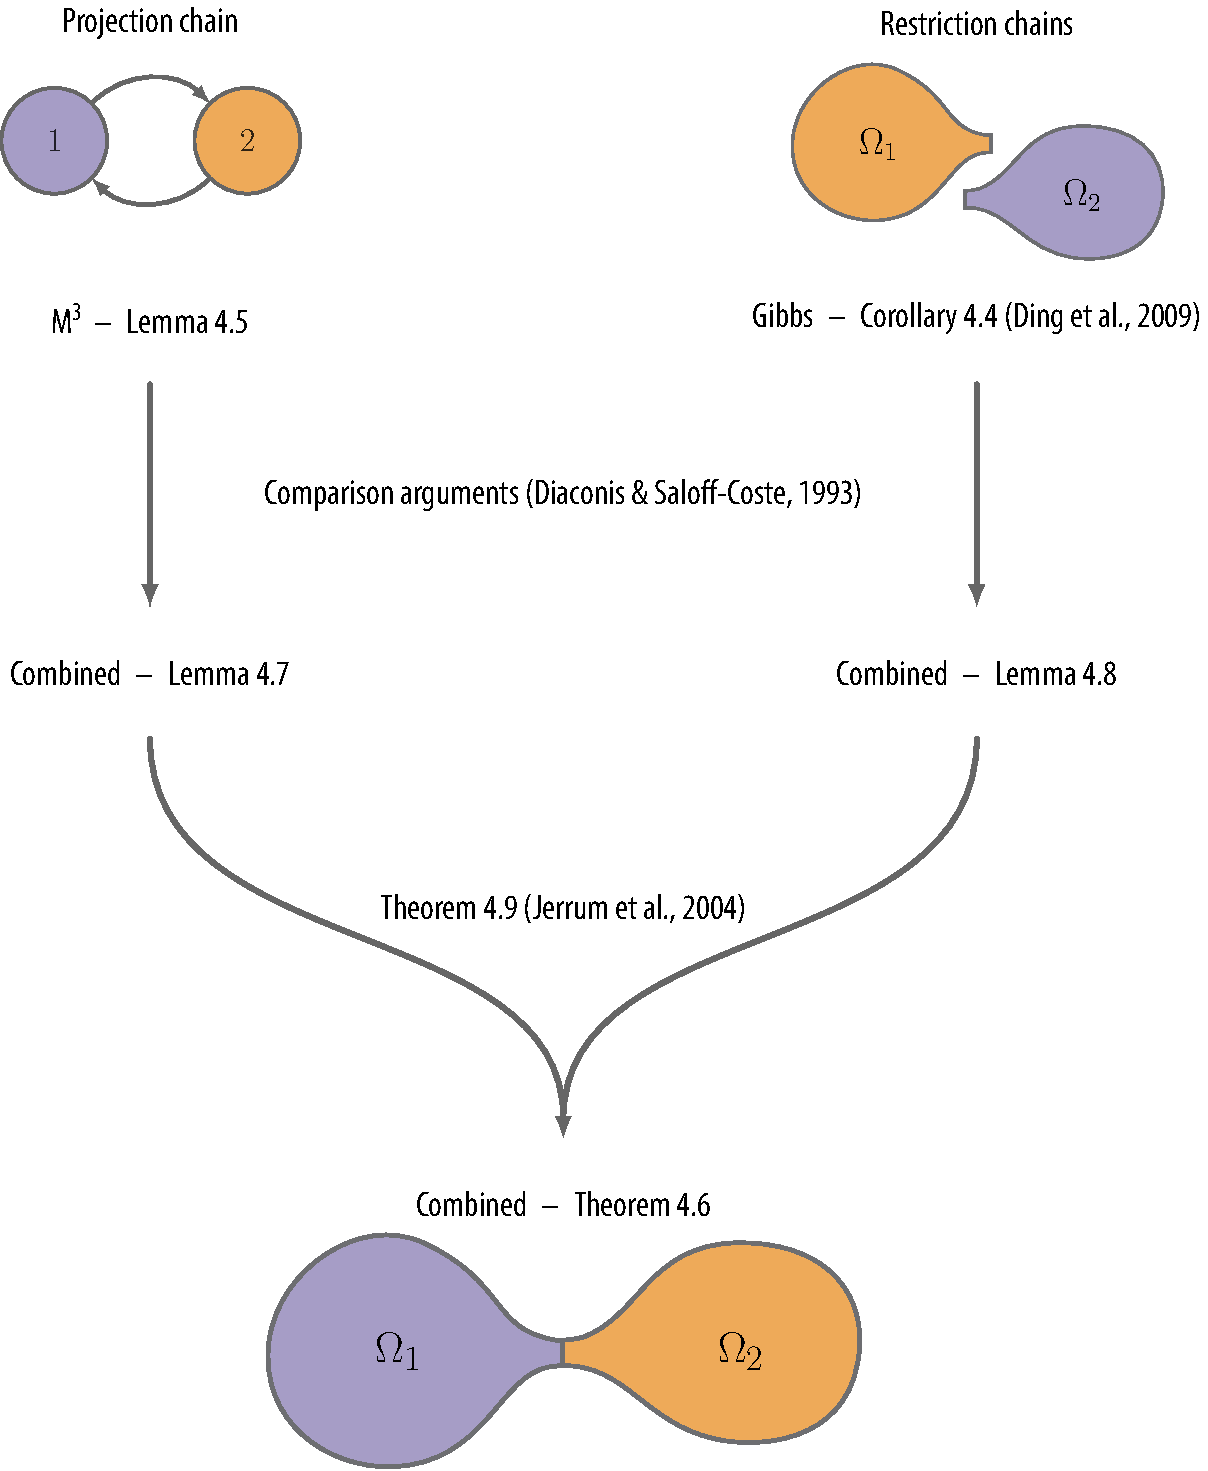
\includegraphics[width=\textwidth]{figures/m3/decomposition2.pdf}\\[2em]
  \caption{The structure of our reasoning to prove \theoremref{thm:combo}.}
  \label{fig:decomp}
\end{figure}

\paragraph{Gibbs restrictions.}
Coming back to the Gibbs sampler, if we could show that it mixes fast within each of $\Omega_0$ and $\Omega_1$, then we could deduce that the only reason for the slow mixing on $\Omega$ is the bottleneck between these two sets.
Indeed, the following corollary of a theorem by \cite{ding09} shows exactly that.
\begin{cor}[cf. Theorem 2, \citealp{ding09}] \label{cor:grest}
  For all $n \geq 3$, the restriction chains of the Gibbs sampler $\Pg_i$, $i = 0, 1$, on \ising{} have spectral gap $\gg_i = \Theta\big(\displaystyle\tfrac{2\ln(n) - 1}{n}\big)$.
\end{cor}

\paragraph{\Ms{} projection.}
To improve mixing we want to create an \Ms{} chain that is able to bypass the aforementioned bottleneck.
For this purpose, we use a mixture of two log-modular distributions, the first of which puts most of its mass on $\Omega_0$, and the second on $\Omega_1$.
We define the mixture of the form \eqref{eq:qprop} by
\begin{align*}
  m_1(S) &= \sum_{v \in S} -\dn (n-1) = -\dn (n-1) |S|,\\
  m_2(S) &= \sum_{v \in S} \dn (n-1) = \dn (n-1) |S|.
\end{align*}
We also use $w_1 = 1 / Z_1$ and $w_2 = 1 / Z_2$, where $Z_1$ and $Z_2$ are the normalizers of $m_1$ and $m_2$ respectively.
The resulting proposal distribution can be written as follows,
\begin{align} \label{eq:qdef}
  q(S) = \frac12\left( \frac{\exp(-\dn (n-1)|S|)}{Z_1} + \frac{\exp(\dn (n-1)|S|)}{Z_2}\right),
\end{align}
where $Z_1 = \left(1 + \exp(-\dn(n-1))\right)^n$, and $Z_2 = \left(1 + \exp(\dn(n-1))\right)^n$.
It follows that $Z_q = 1 / 2$, and, furthermore, the mixture $q$ is symmetric, that is, $q(S) = q(V \setminus S)$.

Since the proposal $q$ is symmetric and state independent, we would expect the \Ms{} chain to jump between $\Omega_0$ and $\Omega_1$ without being hindered by the bottleneck described previously.
We verify this intuition by proving the following lemma.
\begin{lemma} \label{lem:mproj}
  For all $n \geq 10$, the projection chain $\bPm$ of the \Ms{} sampler on \ising{} has spectral gap $\bgm = \Omega(1)$.
\end{lemma}

\begin{proof}
We define $p_k = \sum_{S \in \Omega, |S| = k} p(S)$, and $q_k = \sum_{S \in \Omega, |S| = k} q(S)$.
We then proceed to upper bound $p_k$, and lower bound $q_k$.

\paragraph{Bounding $p_k$.}
By definition, we can write $p_k = \hat{p}_k / Z$, where $\hat{p}_0 = 1$, and for $k > 0$ we have
\begin{align*}
\hat{p}_k &\defeq \binom{n}{k} \exp\left(-\frac{2\ln(n)}{n} k(n-k)\right)\\
            &= \binom{n}{k} n^{-\frac{2k}{n} (n-k)}\\
            &\leq \left(\frac{en}{k}\right)^k n^{-\frac{2k}{n} (n-k)}\\
            &= \left(\frac{e}{k}\right)^k n^{-k + \frac{2k^2}{n}}.
\end{align*}
It follows that
\begin{align} \label{eq:logpk}
  \ln(\hat{p}_k) \leq -k \ln\left(\frac{k}{e}\right) + \left(\frac{2k^2}{n} - k\right)\ln(n).
\end{align}
It is easy to verify that for all $n \geq 10$ and $3 \leq k \leq \lfloor n/2 \rfloor$, it holds that $(2k-n)\ln(n) \leq 0.5n\ln(k/e)$.
Substituting this into \eqref{eq:logpk}, we get
\begin{align*}
            \ln(\hat{p}_k) &\leq -0.5k\ln\left(\frac{k}{e}\right)\\
  \Rightarrow\ \ \hat{p}_k &\leq \exp(-0.5k\ln(k/e)).
\end{align*}
Noting that, for all $k$, $\hat{p}_k \leq 1$, and using the fact that $\hat{p}_{n-k} = \hat{p}_k$, we get
\begin{align}
  Z &= \sum_{k = 0}^n \hat{p}_k \nonumber\\ 
    &\leq 2\sum_{k = 0}^{\lfloor n/2 \rfloor} \hat{p}_ k\nonumber\\
    &= 2(\hat{p}_0 + \hat{p}_1 + \hat{p}_2 + \sum_{k = 3}^{\lfloor n/2 \rfloor} \hat{p}_k) \nonumber\\
    &\leq 3 + \sum_{k = 3}^{\lfloor n/2 \rfloor} \exp(-0.5k\ln(k/e)) \nonumber\\
    &\leq c_1, \label{eq:Zconst}
\end{align}
where $c_1$ is a constant.

\paragraph{Bounding $q_k$.}
First, it is easy to see that, for all $n \geq 1$, $Z_1 \leq 3$.
\begin{align*}
  q_k &= \sum_{S \in \Omega, |S| = k} q(S)\\
      &\geq \sum_{S \in \Omega, |S| = k} \frac{1}{2} \frac{\exp(-\dn (n-1)|S|)}{Z_1} \tag{by \eqref{eq:qdef}} \\
      &\geq \frac{1}{6} \binom{n}{k} \exp(-\dn (n-1)|S|)
\end{align*}

\paragraph{Bounding the spectral gap.}
For the projection chain $\bPm$, we have
\begin{align*}
\bPm(0, 1) &= \frac{1}{\bar{p}(0)} \sum_{\subalign{S &\in \Omega_i\\ R &\in \Omega_j}} p(S) \Pm(S, R)\\
           %&\geq \frac{1}{\bar{p}(0)} \sum_{\subalign{S &\in \Omega_i\\ R &\in \Omega_j\\ |R| &= |V \setminus S|}} p(S) \Pm(S, R)\\
           %&\geq \frac{1}{\bar{p}(0)} \sum_{\subalign{S &\in \Omega_i\\ R &\in \Omega_j\\ |R| &= |V \setminus S|}} p(S) q(R)\displaystyle\frac{p(R)q(S)}{p(S)q(R)}\\ \tag{$p(R) = p(S)$ and $q(R) = q(S)$}
           %&\geq \frac{1}{\bar{p}(0)} \sum_{\subalign{S &\in \Omega_i\\ R &\in \Omega_j\\ |R| &= |V \setminus S|}} p(S) q(R)\\
           %&\geq \frac{1}{\bar{p}(0)} \sum_{k = 0}^{\lfloor n/2 \rfloor} p_k q_{n-k}\\
           %&= \frac{1}{\bar{p}(0)} \sum_{k = 0}^{\lfloor n/2 \rfloor} p_k q_{k} \tag{by symmetry of $q_k$}\\
           %&= 2 \sum_{k = 0}^{\lfloor n/2 \rfloor} p_k q_{k} \tag{$\bar{p}(0) = 1/2$ by symmetry of $p$} \\
           &\geq 2p_0 q_n \tag{$\bar{p}(0) = 1/2$ by symmetry of $p$}\\
           &= 2p_0 q_0 \tag{by symmetry of $q$}\\
           &\geq 2\frac{\hat{p}_0}{Z} \frac{1}{6} \tag{$q_0 \geq \frac{1}{6}$}\\
           &\geq 2\frac{1}{c_1}\frac{1}{6} \tag{$\hat{p}_0 = 1$}\\
           &= c \bar{p}(1),
\end{align*}
where $c = (2/3)c_1$.

Finally, it is easy to show that the spectral gap of any reversible two-state chain $P$ with stationary distribution $p$ that satisfies $P(0, 1) = c\,p(1)$ is $c$; for example, see Fact 6 by \cite{anari16}.
Applying this to the above projection chain shows that the spectral gap of $\bPm$ is $c$.
\end{proof}

\paragraph{Combining the chains.}
Putting everything together, we show the following result about the combined chain $\Pc$.
\begin{theorem} \label{thm:combo}
  For all $n \geq 10$, the combined chain $\Pc$ on \ising{} has spectral gap
  \begin{align*}
    \gc = \Omega\left( \displaystyle\frac{2\ln(n) - 1}{2n} \right).
  \end{align*}
\end{theorem}
\noindent The proof consists of two steps.
In the first step, we make two comparison arguments \citep{diaconis93,levin08book} to show that the spectral gaps of the projection and restriction chains of the combined sampler are smaller by at most a constant factor in $\delta$ compared to those of Gibbs and \Ms{}.
In particular, we use the \Ms{} bound (\lemmaref{lem:mproj}) for the projection chain, and the Gibbs bound (\corref{cor:grest}) for the restriction chains.
The following two lemmas make this more concrete.

\begin{lemma} \label{lem:cproj}
  For all $n \geq 10$, the projection chain $\bPc$ of the combined chain on \ising{} has spectral gap $\bgc = \Omega(1).$
\end{lemma}

\begin{proof}
  By definition, $\bPc(S, R) \geq \delta \bPm(S, R)$, therefore a simple comparison argument (e.g., Lemma 13.22 in \citep{levin08book}) combined with the result of \lemmaref{lem:mproj} gives us $\bgc \geq \delta \bgm = \Omega(1)$.
\end{proof}

\begin{lemma} \label{lem:crest}
  For all $n \geq 3$, each of the restriction chains $\Pc_i$ of the combined chain on \ising{} has spectral gap $\gc_i = \Theta\left(\displaystyle\frac{2\ln(n) - 1}{2n}\right)$.
\end{lemma}

\begin{proof}
  By definition, $\Pc_i(S, R) \geq \delta \Pg_i(S, R)$, therefore, using a comparison argument like above together with \corref{cor:grest} gives us
  \begin{align*}
  \gc_i \geq \delta \gg_i = \Theta\left(\displaystyle\frac{2\ln(n) - 1}{2n}\right).
  \end{align*}
\end{proof}

The second step combines the projection and restriction bounds to establish a bound on the spectral gap of the combined chain.
To accomplish this we use the following result by \cite{jerrum04poincare}, which states that the spectral gap of the whole chain cannot be much smaller than the smallest of the projection and restriction spectral gaps.
\begin{theorem}[\hspace{1sp}Theorem 1, \citealp{jerrum04poincare}] \label{thm:jerrum04}
  Given a reversible Markov chain $P$, if the spectral gap of its projection chain $\bar{P}$ is bounded below by $\bar{\gamma}$, and the spectral gaps of its restriction chains $P_i$ are uniformly bounded below by $\gamma_{\textrm{min}}$, then the spectral gap of $P$ is bounded below by
  \begin{align*}
    \gamma = \min\left\{ \frac{\bar{\gamma}}{3}, \frac{\bar{\gamma}\gamma_{\textrm{min}}}{3\Pmax + \bar{\gamma}} \right\},
  \end{align*}
  where $p_{\textrm{max}} \defeq \displaystyle\max_{i \in \{0, 1\}}\max_{S \in \Omega_i} \sum_{R \in \Omega \setminus \Omega_i} P(S, R)$.
\end{theorem}

The result of \theoremref{thm:combo} follows directly by combining the spectral gap bounds of \lemmasref{lem:cproj} and \ref{lem:crest} in \theoremref{thm:jerrum04}, and noting that $\Pmax \leq 1$.

Finally, using \theoremref{thm:spectral}, and noting that, in this case, $\pmin = \bO(e^{-n})$ (cf. proof of \lemmaref{lem:mproj}), we get a mixing time of $\tme = \bO(n^2 \log(1 / \epsilon))$ for the combined chain.
This shows that the addition of the \Ms{} sampler results in an exponential improvement in mixing time over the Gibbs sampler by itself.

\section{Constructing the Mixture}
Having seen the positive effect of the \Ms{} sampler, we now turn to the issue of how to choose the proposal $q$.
While a manual construction like the one we just presented for the Ising model may be feasible in some cases, it is often more practical to have an automated way of obtaining the mixture.

Let us assume, as is usually the case, that we have access to a function oracle for $F$, and we want to create a mixture of size $r$.
Ideally, we would like to construct a proposal $q$ that is as close to $p$ as possible, that is, minimize an objective such as the following,
\begin{align*}
  E_1(q) &\defeq \min_q \| p - q \|\\
         &\,\,= \min_q \left\| \frac{\exp(F(\cdot))}{Z} - \frac{1}{Z_q}\textstyle\sum_{i = 1}^r \wi\exp(\mi(\cdot)) \right\|,
\end{align*}
where $\| \cdot \|$ could be, for example, total variation distance or the maximum norm.
Unfortunately, this problem is hard: both computing the partition function $Z$, and jointly optimizing over all $\wi, \mi$ are infeasible in practice.
To make the problem easier, we could try to get rid of the normalizers and weights $\wi$, and iteratively minimize over each $\mi$ individually:
\begin{align*}
  E_2^{(i)}(m_i) \defeq \min_{m_i} \left\| \exp(F(\cdot)) - \textstyle\sum_{j = 1}^{i-1} \exp(\mi(\cdot)) \right\|,
\end{align*}
for $i \in \{1, \ldots, r\}$.
This problem is still hard, since optimizing $\| \exp(F(\cdot)) \|$ is by itself infeasible in general.

\begin{algorithm}[tb]
  \setstretch{1.3}
  \DontPrintSemicolon
  \caption{\strut Iterative semigradient-based mixture construction}
  \label{alg:mixture}
  \vspace{0.5em}
  \SetKwInOut{Input}{Input}
  \Input{Set function $F$, mixture size $r$}
  \For{$i = 1$ \KwTo $r$}{
  $\sigma$ $\gets$ \textsc{GreedyDifMax}($F$, $\{m_1, \ldots, m_{i-1}\}$) \label{lin:perm}\;
  $m_i$ $\gets$ \textsc{SemiGradient}($F$, $\sigma$)\;
  }
  \Return{$\{m_1, \ldots, m_r\}$}\;
\end{algorithm}

\begin{algorithm}[tb]
  \setstretch{1.3}
  \DontPrintSemicolon
  \caption{\strut Greedy difference maximization}
  \label{alg:greedy_dif}
  \vspace{0.5em}
  \SetKwInOut{Input}{Input}
  \Input{Set function $F$, modular functions $\{m_1, \ldots, m_{i-1}\}$}
  $D_i(S)$ $\gets$ $F(S) - \log \sum_{j=1}^{i-1} \exp(m_j(S))$, for all $S \in \Omega$\;
  $\sigma$ $\gets$ $(1, \ldots, n)$\;
  $A$ $\gets$ $\varnothing$\;
  \For{$i = 1$ \KwTo $n$}{
  $v^*$ $\gets$ $\argmax_{v \in V \setminus A} \left( D_i(A \cup \{v\}) - D_i(A) \right)$\;
  $\sigma_i$ $\gets$ $v^*$\;
  $A$ $\gets$ $A \cup \{v^*\}$\;
  }
  \Return{$\sigma$}\;
\end{algorithm}

To arrive at a practical algorithm, we approximate the above objective using the two-step procedure described in \algoref{alg:mixture}.
In the first step, we generate a permutation $\sigma$ of the ground set $V$ by running the greedy algorithm on function $D_i(S) \defeq F(S) - \log \sum_{j=1}^{i-1} \exp(m_j(S))$, as shown in \algoref{alg:greedy_dif}.
Intuitively, the sets that are formed by elements near the beginning of $\sigma$ are those on which $F$ and the current mixture disagree by the most.
Therefore, in the second step, we would like to add to the mixture a modular function $\mi$ that is a good approximation for $F$ on $\{\sigma_1, \ldots, \sigma_k\}$, for a choice of $1 \leq k \leq n$.
To accomplish this, we propose using discrete semigradients.

Semigradients are modular functions that provide lower (subgradient) or upper (supergradient) approximations of a set function $F$ \citep{fujishige05,iyer13}.
More concretely, given a set $S \in \Omega$, a modular function $m$ is a subgradient of $F$ at $S$, if, for all $R \in \Omega$, $F(R) \geq F(S) + m(R) - m(S)$.
Similarly, $m$ is a supergradient if the inequality is reversed.
Although, in general, a function is not guaranteed to have sub- or supergradients at each $S \in \Omega$, it has been shown that this is true when $F$ is submodular or supermodular \citep{fujishige05, jegelka11, iyer12}.

Coming back to the second step of \algoref{alg:mixture}, to create a subgradient of $F$ given permutation $\sigma$ we just need to define a modular function via marginal gains according to the permutation order \citep{iyer13}, as shown in \algoref{alg:sub}.
Moreover, this is a subgradient of $F$ at $\{\sigma_1, \ldots, \sigma_k\}$, for all $1 \leq k \leq n$.
On the other hand, \algoref{alg:super} creates a supergradient of $F$ at $\{\sigma_1, \ldots, \sigma_k\}$ for a randomly chosen $k$. (This type of supergradient is denoted by $\bar{g}_Y$ by \cite{iyer13}.)
In fact, the modular functions $m_1$, $m_2$ that we used in analyzing the Ising model in the previous section were supergradients of $F$ at sets $S_1 = \varnothing$, and $S_2 = V$ respectively.

\begin{algorithm}[tb]
  \setstretch{1.3}
  \DontPrintSemicolon
  \caption{\strut Subgradient computation}
  \label{alg:sub}
  \vspace{0.5em}
  \SetKwInOut{Input}{Input}
  \Input{Set function $F$, permutation $\sigma$}
  $A$ $\gets$ $\varnothing$\;
  $c$ $\gets$ $F(\varnothing)$\;
  \For{$v = 1$ \KwTo $n$}{
    $m_v$ $\gets$ $F(A \cup \{\sigma_v\}) - F(A)$\;
    $A$ $\gets$ $A \cup \sigma_v$\;
  }
  \Return{$m(S) \defeq c + \sum_{v \in S} m_v$}\;% \textrm{, for all} $S \in \Omega$}\;
\end{algorithm}

\begin{algorithm}[tb]
  \setstretch{1.3}
  \DontPrintSemicolon
  \caption{\strut Supergradient computation}
  \label{alg:super}
  \vspace{0.5em}
  \SetKwInOut{Input}{Input}
  \Input{Set function $F$, permutation $\sigma$}
  Draw $k \sim \mathrm{Unif}(\{1,\ldots,n\})$\;
  \For{$v = 1$ \KwTo $k$}{
    $m_v$ $\gets$ $F(V) - F(V \setminus \{v\})$
  }
  \For{$v = k+1$ \KwTo $n$}{
    $m_v$ $\gets$ $F(\{v\})$
  }
  \Return{$m(S) \defeq \sum_{v \in S} m_v$}
\end{algorithm}

In practice, we can use \algoref{alg:mixture} regardless of whether $F$ is sub- or supermodular.
We have noticed that subgradients give better results when $F$ is submodular, and vice versa for supergradients and supermodular $F$.


\section{Experiments}
We start by repeating the experiment of the previous chapter shown in \figref{fig:gibbs_zest}, which involved estimating the log-partition function using reverse importance sampling on a synthetic data set that contains a group of three mutually exclusive genes.
Here we only focus on the ground set of size $|V| = 100$.
\figref{fig:exp3} shows the resulting (approximate) error in estimating $\log(Z)$ using the Gibbs sampler, compared to our proposed combined sampler using a mixture $q$ constructed by \algoref{alg:mixture} (\textsf{Combo-I}).
We also compare against a variation where we substitute the greedy procedure in \lineref{lin:perm} of \algoref{alg:mixture} with picking a permutation $\sigma$ of the ground set uniformly at random (\textsf{Combo-R}).
Both variations use $r = 20$ subgradients, and we repeat the experiment $100$ times.
We can see that they clearly outperform the Gibbs sampler, while the difference between the two variations is not as significant.

\setlength\figureheight{0.65\textwidth}
\setlength\figurewidth{0.9\textwidth}
\begin{figure}[tb]
  \centering
  \begin{tikzpicture}


\begin{axis}[%
tick label style={/pgf/number format/fixed,font=\sffamily},
label style={font=\sffamily},
legend style={font=\sffamily},
view={0}{90},
width=\figurewidth,
height=\figureheight,
xmin=0, xmax=5000,
xtick={0, 1000, 2000, 3000, 4000, 5000},
xticklabels={0, 1k, 2k, 3k, 4k, 5k},
scaled x ticks=false,
xlabel={Samples},
xlabel shift=0em,
ymin=0, ymax=0.8,
ytick={0, 0.4, 0.8},
yticklabels={0, 0.4, 0.8},
ylabel={log-partition error},
ylabel shift=0em,
major tick length=2pt,
axis lines*=left,
legend cell align=left,
clip marker paths=true,
legend style={anchor=north east,at={(1,1)},draw=none,row sep=0em},
every axis plot/.append style={
  line width=1.5pt,
  opacity=0.8,
}
]

\addplot [
color=gcol1,
densely dashed
]
coordinates{
(100,0.74943)+-(0.03564,0.03564)(250,0.45015)+-(0.03204,0.03204)(500,0.34592)+-(0.02861,0.02861)(1000,0.26464)+-(0.02428,0.02428)(2000,0.17517)+-(0.02049,0.02049)(3000,0.13932)+-(0.01993,0.01993)(4000,0.13965)+-(0.01738,0.01738)(5000,0.10302)+-(0.01854,0.01854)
};
\addlegendentry{\textsc{Gibbs}}


\addplot [
color=gcol2
]
coordinates{
(100,0.26654)+-(0.00793,0.00793)(250,0.17668)+-(0.00676,0.00676)(500,0.13299)+-(0.00578,0.00578)(1000,0.09522)+-(0.00498,0.00498)(2000,0.06694)+-(0.00427,0.00427)(3000,0.05462)+-(0.00383,0.00383)(4000,0.04396)+-(0.00360,0.00360)(5000,0.04151)+-(0.00332,0.00332)
};
\addlegendentry{Combo-R}


\addplot [
color=gcol3
]
coordinates{
(100,0.21765)+-(0.09712,0.09712)(250,0.15303)+-(0.06441,0.06441)(500,0.09433)+-(
0.06863,0.06863)(1000,0.07503)+-(0.04443,0.04443)(2000,0.05652)+-(0.05006,0.0500
6)(3000,0.01747)+-(0.03893,0.03893)(4000,0.03384)+-(0.03219,0.03219)(5000,0.0281
6)+-(0.03372,0.03372)
};
\addlegendentry{Combo-I}

\end{axis}
\end{tikzpicture}

  \caption{The error in estimating the log-partition function with the two versions of the combined sampler compared to the Gibbs sampler.}
  \label{fig:exp3}
\end{figure}

Next we evaluate the marginal inference performance of our proposed sampler on the Ising model we analyzed earlier, as well as the following three models learned from real-world data sets.
\paragraph{\textsf{Water}.} The same \flid{} model that we used in the experimental section of last chapter (see \figref{fig:gibbs_exp1}), which was based on a problem of sensor placement in a water distribution network \citep{krause08}
In this case, we randomly subsample the original facility location matrix, so that $n = 50$, and $L = 500$.

\paragraph{\textsf{Sensor}.} A determinantal point process (see \exampleref{ex:dpp}), which was used in a problem of sensor placement for indoor temperature monitoring \citep{guestrin05}.
The function $F$ is of the form
\begin{align*}
F(S) = \log |K + \sigma^2 I|,
\end{align*}
where $K$ is a kernel matrix, and $\sigma$ is a noise parameter.
The size of the ground set is $n = 46$.

\paragraph{\textsf{Game}.} A \flid{} model that represents the characters that are chosen by players in the popular online game ``Heroes of the Storm''.
We learned the model from an online data set of approximately $8,000$ teams of $5$ characters\footnote{https://www.hotslogs.com} using noise-contrastive estimation, as described by \cite{tschiatschek16}.
The model has a ground set of size $n = 48$, and $L = 10$ latent dimensions.

In practice, we would only be interested in sampling sets of fixed size $\ell = 5$.
The Gibbs sampler can be easily modified to sample under a cardinality constraint by using moves that swap an element in the current set $X_t$ with an element in $V \setminus X_t$.
Extending the \Ms{} chain to sample from cardinality-constrained models is also straightforward.
In fact, the only additional ingredient required is a procedure to sample a set of size $\ell$ from a log-modular distribution, which can be easily done, as before, in $\bO(n)$ time.

\paragraph{Results.}
To assess convergence, we use the potential scale reduction factor (PSRF) \citep{brooks11} with $20$ parallel chains.
Intuitively, the PSRF compares the within-chain variance of some probabilistic quantity to the between-chain variance of that same quantity.
As each of the chains converges to the stationary distribution, the PSRF is expected to converge to $0$.
In our experiments, we compute the PSRF using single-element marginal probabilities, and show the worst (highest PSRF) marginal averaged over $50$ repetitions of each simulation.

In \figref{fig:expising} we show the results for the Ising model ($n = 6, 7, 8$).
The additional \textsc{Combo-f} line denotes the combined sampler with two mixture components discussed in \sectref{sect:ising}.
The other two combined samplers use mixtures of size $r = 20$.
Note that Gibbs mixes dramatically slower than the combined sampler, even for such small $n$, because of the significant bottleneck we described before.

\setlength\figureheight{0.47\textwidth}
\setlength\figurewidth{0.65\textwidth}
\renewcommand{\subflen}{1.0\textwidth}
\begin{figure}[htbp]
  \begin{subfigure}[b]{\subflen}
    \centering
    \begin{tikzpicture}

\begin{axis}[%
tick label style={/pgf/number format/fixed,font=\sffamily\small},
label style={font=\sffamily\small},
legend style={font=\sffamily\small},
view={0}{90},
width=\figurewidth,
height=\figureheight,
xmin=0, xmax=10000,
xtick={0, 2000, 4000, 6000, 8000, 10000},
xticklabels={0, 2k, 4k, 6k, 8k, 10k},
scaled x ticks=false,
xlabel={Samples},
xlabel shift=0em,
ymin=1, ymax=1.52,
ytick={1, 1.5},
yticklabels={1, 1.5},
ylabel={PSRF},
ylabel shift=-1em,
major tick length=2pt,
axis lines*=left,
legend cell align=left,
clip marker paths=true,
legend style={anchor=north east,at={(1,1)},draw=none,row sep=0em},
every axis plot/.append style={
  line width=1.5pt,
  opacity=0.8,
}
]

\addplot [
color=gcol1,
densely dashed
]
coordinates{
(100,3.378099) +- (-0.282843,0.282843)(150,2.938422) +- (-0.151760,0.151760)(200,2.532023) +- (-0.159217,0.159217)(250,2.261538) +- (-0.111451,0.111451)(300,2.054314) +- (-0.092123,0.092123)(350,1.874944) +- (-0.070360,0.070360)(400,1.767087) +- (-0.064088,0.064088)(450,1.681454) +- (-0.065038,0.065038)(500,1.592597) +- (-0.053144,0.053144)(550,1.543078) +- (-0.046912,0.046912)(600,1.511899) +- (-0.046000,0.046000)(650,1.486062) +- (-0.044927,0.044927)(700,1.457672) +- (-0.041328,0.041328)(750,1.430176) +- (-0.035585,0.035585)(800,1.401466) +- (-0.030985,0.030985)(850,1.375708) +- (-0.029948,0.029948)(900,1.345175) +- (-0.026733,0.026733)(950,1.315470) +- (-0.026751,0.026751)(1000,1.293519) +- (-0.025797,0.025797)(1000,1.293519) +- (-0.025797,0.025797)(1200,1.251332) +- (-0.026475,0.026475)(1400,1.213421) +- (-0.019653,0.019653)(1600,1.179927) +- (-0.016185,0.016185)(1800,1.152976) +- (-0.013040,0.013040)(2000,1.139469) +- (-0.012673,0.012673)(2200,1.125057) +- (-0.012795,0.012795)(2400,1.112741) +- (-0.008976,0.008976)(2600,1.107873) +- (-0.008505,0.008505)(2800,1.100164) +- (-0.008471,0.008471)(3000,1.092954) +- (-0.008492,0.008492)(3200,1.089254) +- (-0.007482,0.007482)(3400,1.080773) +- (-0.006507,0.006507)(3600,1.075257) +- (-0.006793,0.006793)(3800,1.074780) +- (-0.007282,0.007282)(4000,1.072297) +- (-0.007637,0.007637)(4200,1.067025) +- (-0.006494,0.006494)(4400,1.065540) +- (-0.006410,0.006410)(4600,1.062918) +- (-0.005352,0.005352)(4800,1.059046) +- (-0.004797,0.004797)(5000,1.057516) +- (-0.004167,0.004167)(5200,1.055310) +- (-0.003949,0.003949)(5400,1.053404) +- (-0.004055,0.004055)(5600,1.052183) +- (-0.003841,0.003841)(5800,1.051552) +- (-0.003584,0.003584)(6000,1.050591) +- (-0.003938,0.003938)(6200,1.047492) +- (-0.004053,0.004053)(6400,1.044872) +- (-0.003768,0.003768)(6600,1.043283) +- (-0.003739,0.003739)(6800,1.041803) +- (-0.003703,0.003703)(7000,1.040122) +- (-0.003554,0.003554)(7200,1.038240) +- (-0.003463,0.003463)(7400,1.036134) +- (-0.003056,0.003056)(7600,1.034900) +- (-0.002855,0.002855)(7800,1.034405) +- (-0.002825,0.002825)(8000,1.032886) +- (-0.002893,0.002893)(8200,1.031770) +- (-0.002710,0.002710)(8400,1.031264) +- (-0.002854,0.002854)(8600,1.030591) +- (-0.002817,0.002817)(8800,1.029803) +- (-0.002770,0.002770)(9000,1.029227) +- (-0.002713,0.002713)(9200,1.028724) +- (-0.002527,0.002527)(9400,1.028041) +- (-0.002393,0.002393)(9600,1.027631) +- (-0.002233,0.002233)(9800,1.027045) +- (-0.002216,0.002216)(10000,1.025711) +- (-0.002096,0.002096)
};
\addlegendentry{\textsc{Gibbs}}


\addplot [
color=gcol2
]
coordinates{
(100,1.245774) +- (-0.033535,0.033535)(150,1.160920) +- (-0.020011,0.020011)(200,1.109728) +- (-0.010276,0.010276)(250,1.086212) +- (-0.007441,0.007441)(300,1.073510) +- (-0.006756,0.006756)(350,1.064314) +- (-0.005584,0.005584)(400,1.053786) +- (-0.003881,0.003881)(450,1.048140) +- (-0.004670,0.004670)(500,1.038634) +- (-0.002423,0.002423)(550,1.035454) +- (-0.002357,0.002357)(600,1.033217) +- (-0.002506,0.002506)(650,1.030281) +- (-0.002513,0.002513)(700,1.027761) +- (-0.002301,0.002301)(750,1.027078) +- (-0.002488,0.002488)(800,1.024988) +- (-0.002331,0.002331)(850,1.024239) +- (-0.001891,0.001891)(900,1.022156) +- (-0.001505,0.001505)(950,1.020619) +- (-0.001627,0.001627)(1000,1.019861) +- (-0.001773,0.001773)(1000,1.019861) +- (-0.001773,0.001773)(1200,1.016820) +- (-0.001244,0.001244)(1400,1.014436) +- (-0.001055,0.001055)(1600,1.012749) +- (-0.000940,0.000940)(1800,1.011177) +- (-0.000761,0.000761)(2000,1.009927) +- (-0.000671,0.000671)(2200,1.008491) +- (-0.000571,0.000571)(2400,1.008012) +- (-0.000392,0.000392)(2600,1.007707) +- (-0.000417,0.000417)(2800,1.007143) +- (-0.000457,0.000457)(3000,1.006990) +- (-0.000413,0.000413)(3200,1.006346) +- (-0.000359,0.000359)(3400,1.006063) +- (-0.000338,0.000338)(3600,1.005638) +- (-0.000347,0.000347)(3800,1.005349) +- (-0.000345,0.000345)(4000,1.004896) +- (-0.000340,0.000340)(4200,1.004804) +- (-0.000285,0.000285)(4400,1.004610) +- (-0.000316,0.000316)(4600,1.004518) +- (-0.000303,0.000303)(4800,1.004272) +- (-0.000314,0.000314)(5000,1.004110) +- (-0.000288,0.000288)(5200,1.003938) +- (-0.000245,0.000245)(5400,1.003713) +- (-0.000212,0.000212)(5600,1.003553) +- (-0.000216,0.000216)(5800,1.003460) +- (-0.000207,0.000207)(6000,1.003411) +- (-0.000193,0.000193)(6200,1.003324) +- (-0.000225,0.000225)(6400,1.003243) +- (-0.000202,0.000202)(6600,1.003171) +- (-0.000187,0.000187)(6800,1.003077) +- (-0.000180,0.000180)(7000,1.002930) +- (-0.000182,0.000182)(7200,1.002898) +- (-0.000168,0.000168)(7400,1.002849) +- (-0.000186,0.000186)(7600,1.002778) +- (-0.000183,0.000183)(7800,1.002698) +- (-0.000179,0.000179)(8000,1.002621) +- (-0.000175,0.000175)(8200,1.002526) +- (-0.000173,0.000173)(8400,1.002442) +- (-0.000167,0.000167)(8600,1.002387) +- (-0.000161,0.000161)(8800,1.002376) +- (-0.000166,0.000166)(9000,1.002282) +- (-0.000153,0.000153)(9200,1.002204) +- (-0.000155,0.000155)(9400,1.002200) +- (-0.000154,0.000154)(9600,1.002114) +- (-0.000145,0.000145)(9800,1.002087) +- (-0.000136,0.000136)(10000,1.002027) +- (-0.000124,0.000124)
};
\addlegendentry{\textsc{Combo-R}}


\addplot [
color=gcol3
]
coordinates{
(100,1.346909) +- (-0.036826,0.036826)(150,1.200930) +- (-0.015355,0.015355)(200,1.145036) +- (-0.014122,0.014122)(250,1.107371) +- (-0.008610,0.008610)(300,1.089872) +- (-0.006056,0.006056)(350,1.075572) +- (-0.005809,0.005809)(400,1.066123) +- (-0.004161,0.004161)(450,1.057875) +- (-0.003989,0.003989)(500,1.051135) +- (-0.003911,0.003911)(550,1.047260) +- (-0.002989,0.002989)(600,1.044577) +- (-0.003433,0.003433)(650,1.041867) +- (-0.003330,0.003330)(700,1.038111) +- (-0.003005,0.003005)(750,1.035853) +- (-0.002558,0.002558)(800,1.033717) +- (-0.002574,0.002574)(850,1.032791) +- (-0.002601,0.002601)(900,1.030495) +- (-0.002440,0.002440)(950,1.028133) +- (-0.002260,0.002260)(1000,1.026836) +- (-0.002045,0.002045)(1000,1.026836) +- (-0.002045,0.002045)(1200,1.022948) +- (-0.001406,0.001406)(1400,1.019134) +- (-0.001063,0.001063)(1600,1.017185) +- (-0.001150,0.001150)(1800,1.015185) +- (-0.000983,0.000983)(2000,1.013325) +- (-0.000945,0.000945)(2200,1.012275) +- (-0.000836,0.000836)(2400,1.011077) +- (-0.000846,0.000846)(2600,1.009959) +- (-0.000719,0.000719)(2800,1.009164) +- (-0.000653,0.000653)(3000,1.009077) +- (-0.000666,0.000666)(3200,1.008668) +- (-0.000673,0.000673)(3400,1.008168) +- (-0.000633,0.000633)(3600,1.007867) +- (-0.000621,0.000621)(3800,1.007480) +- (-0.000528,0.000528)(4000,1.006745) +- (-0.000498,0.000498)(4200,1.006737) +- (-0.000481,0.000481)(4400,1.006562) +- (-0.000442,0.000442)(4600,1.006253) +- (-0.000423,0.000423)(4800,1.005926) +- (-0.000413,0.000413)(5000,1.005456) +- (-0.000388,0.000388)(5200,1.005277) +- (-0.000376,0.000376)(5400,1.005025) +- (-0.000353,0.000353)(5600,1.004772) +- (-0.000320,0.000320)(5800,1.004524) +- (-0.000332,0.000332)(6000,1.004534) +- (-0.000352,0.000352)(6200,1.004355) +- (-0.000328,0.000328)(6400,1.004231) +- (-0.000331,0.000331)(6600,1.004111) +- (-0.000330,0.000330)(6800,1.003869) +- (-0.000308,0.000308)(7000,1.003742) +- (-0.000276,0.000276)(7200,1.003613) +- (-0.000289,0.000289)(7400,1.003568) +- (-0.000258,0.000258)(7600,1.003527) +- (-0.000235,0.000235)(7800,1.003379) +- (-0.000233,0.000233)(8000,1.003240) +- (-0.000226,0.000226)(8200,1.003186) +- (-0.000227,0.000227)(8400,1.003065) +- (-0.000217,0.000217)(8600,1.002903) +- (-0.000189,0.000189)(8800,1.002855) +- (-0.000174,0.000174)(9000,1.002832) +- (-0.000185,0.000185)(9200,1.002703) +- (-0.000165,0.000165)(9400,1.002623) +- (-0.000163,0.000163)(9600,1.002542) +- (-0.000151,0.000151)(9800,1.002535) +- (-0.000142,0.000142)(10000,1.002501) +- (-0.000135,0.000135)
};
\addlegendentry{\textsc{Combo-I}}


\addplot [
color=gcol4
]
coordinates{
(100,1.167109) +- (-0.027878,0.027878)(150,1.102454) +- (-0.012394,0.012394)(200,1.078688) +- (-0.008910,0.008910)(250,1.063416) +- (-0.007208,0.007208)(300,1.049136) +- (-0.004693,0.004693)(350,1.040569) +- (-0.003381,0.003381)(400,1.035484) +- (-0.003283,0.003283)(450,1.032803) +- (-0.003334,0.003334)(500,1.028276) +- (-0.002731,0.002731)(550,1.027382) +- (-0.002881,0.002881)(600,1.025636) +- (-0.002789,0.002789)(650,1.022359) +- (-0.002361,0.002361)(700,1.020696) +- (-0.001862,0.001862)(750,1.019722) +- (-0.001640,0.001640)(800,1.018251) +- (-0.001516,0.001516)(850,1.016289) +- (-0.001461,0.001461)(900,1.016462) +- (-0.001700,0.001700)(950,1.016098) +- (-0.001628,0.001628)(1000,1.015015) +- (-0.001380,0.001380)(1000,1.015015) +- (-0.001380,0.001380)(1200,1.013406) +- (-0.001161,0.001161)(1400,1.010840) +- (-0.000956,0.000956)(1600,1.009103) +- (-0.000637,0.000637)(1800,1.007829) +- (-0.000706,0.000706)(2000,1.007327) +- (-0.000517,0.000517)(2200,1.006347) +- (-0.000406,0.000406)(2400,1.005852) +- (-0.000404,0.000404)(2600,1.005511) +- (-0.000387,0.000387)(2800,1.005048) +- (-0.000333,0.000333)(3000,1.004469) +- (-0.000345,0.000345)(3200,1.004287) +- (-0.000304,0.000304)(3400,1.004014) +- (-0.000279,0.000279)(3600,1.003876) +- (-0.000252,0.000252)(3800,1.003830) +- (-0.000266,0.000266)(4000,1.003727) +- (-0.000247,0.000247)(4200,1.003600) +- (-0.000276,0.000276)(4400,1.003388) +- (-0.000244,0.000244)(4600,1.003196) +- (-0.000199,0.000199)(4800,1.003092) +- (-0.000184,0.000184)(5000,1.002929) +- (-0.000159,0.000159)(5200,1.002904) +- (-0.000143,0.000143)(5400,1.002731) +- (-0.000140,0.000140)(5600,1.002553) +- (-0.000123,0.000123)(5800,1.002522) +- (-0.000146,0.000146)(6000,1.002494) +- (-0.000149,0.000149)(6200,1.002358) +- (-0.000170,0.000170)(6400,1.002312) +- (-0.000148,0.000148)(6600,1.002236) +- (-0.000155,0.000155)(6800,1.002144) +- (-0.000146,0.000146)(7000,1.002133) +- (-0.000138,0.000138)(7200,1.002031) +- (-0.000122,0.000122)(7400,1.001990) +- (-0.000121,0.000121)(7600,1.001909) +- (-0.000125,0.000125)(7800,1.001884) +- (-0.000126,0.000126)(8000,1.001830) +- (-0.000124,0.000124)(8200,1.001787) +- (-0.000127,0.000127)(8400,1.001740) +- (-0.000116,0.000116)(8600,1.001684) +- (-0.000093,0.000093)(8800,1.001597) +- (-0.000086,0.000086)(9000,1.001551) +- (-0.000084,0.000084)(9200,1.001536) +- (-0.000076,0.000076)(9400,1.001547) +- (-0.000070,0.000070)(9600,1.001504) +- (-0.000067,0.000067)(9800,1.001491) +- (-0.000070,0.000070)(10000,1.001479) +- (-0.000078,0.000078)
};
\addlegendentry{\textsc{Combo-F}}

\end{axis}
\end{tikzpicture}
    \vspace{-0.5em}
    \caption{\textsf{Ising} ($n = 6$)}
    \label{fig:ising6}
  \end{subfigure}\\[1em]
  \begin{subfigure}[b]{\subflen}
    \centering
    \begin{tikzpicture}

\begin{axis}[%
tick label style={/pgf/number format/fixed,font=\sffamily\small},
label style={font=\sffamily\small},
legend style={font=\sffamily\small},
view={0}{90},
width=\figurewidth,
height=\figureheight,
xmin=0, xmax=10000,
xtick={0, 2000, 4000, 6000, 8000, 10000},
xticklabels={0, 2k, 4k, 6k, 8k, 10k},
scaled x ticks=false,
xlabel={Samples},
xlabel shift=-0.3em,
ymin=1, ymax=1.52,
ytick={1, 1.5},
yticklabels={1, 1.5},
ylabel={PSRF},
ylabel shift=-1.1em,
major tick length=2pt,
axis lines*=left,
legend cell align=left,
clip marker paths=true,
legend style={anchor=north east,at={(1,1)},draw=none,row sep=0em},
every axis plot/.append style={
  line width=1.5pt,
  opacity=0.8,
}
]

\addplot [
color=col1dark,
densely dashed
]
coordinates{
(100,3.896208) +- (-0.282843,0.282843)(150,3.739615) +- (-0.282843,0.282843)(200,3.642484) +- (-0.282843,0.282843)(250,3.557257) +- (-0.282843,0.282843)(300,3.178533) +- (-0.277385,0.277385)(350,2.974985) +- (-0.227180,0.227180)(400,2.708438) +- (-0.190721,0.190721)(450,2.561393) +- (-0.192645,0.192645)(500,2.463448) +- (-0.173053,0.173053)(550,2.337529) +- (-0.148764,0.148764)(600,2.218182) +- (-0.120421,0.120421)(650,2.165834) +- (-0.107972,0.107972)(700,2.109161) +- (-0.107845,0.107845)(750,2.058582) +- (-0.106084,0.106084)(800,2.000832) +- (-0.099719,0.099719)(850,1.937352) +- (-0.087618,0.087618)(900,1.872072) +- (-0.082553,0.082553)(950,1.812060) +- (-0.081620,0.081620)(1000,1.755994) +- (-0.073638,0.073638)(1000,1.755994) +- (-0.073638,0.073638)(1200,1.587606) +- (-0.050434,0.050434)(1400,1.495127) +- (-0.039021,0.039021)(1600,1.444903) +- (-0.036102,0.036102)(1800,1.395842) +- (-0.030115,0.030115)(2000,1.342865) +- (-0.026348,0.026348)(2200,1.305323) +- (-0.023374,0.023374)(2400,1.280074) +- (-0.022377,0.022377)(2600,1.266798) +- (-0.023385,0.023385)(2800,1.246877) +- (-0.023293,0.023293)(3000,1.239355) +- (-0.023334,0.023334)(3200,1.227831) +- (-0.022143,0.022143)(3400,1.215640) +- (-0.021151,0.021151)(3600,1.200760) +- (-0.020098,0.020098)(3800,1.189016) +- (-0.019135,0.019135)(4000,1.178751) +- (-0.019408,0.019408)(4200,1.168659) +- (-0.017415,0.017415)(4400,1.155525) +- (-0.015521,0.015521)(4600,1.146588) +- (-0.014234,0.014234)(4800,1.139240) +- (-0.013193,0.013193)(5000,1.131557) +- (-0.012880,0.012880)(5200,1.123362) +- (-0.011860,0.011860)(5400,1.116154) +- (-0.010758,0.010758)(5600,1.110660) +- (-0.009586,0.009586)(5800,1.108292) +- (-0.008875,0.008875)(6000,1.105119) +- (-0.008731,0.008731)(6200,1.100983) +- (-0.008110,0.008110)(6400,1.097247) +- (-0.007703,0.007703)(6600,1.094453) +- (-0.007182,0.007182)(6800,1.093285) +- (-0.006628,0.006628)(7000,1.090694) +- (-0.006238,0.006238)(7200,1.087508) +- (-0.005763,0.005763)(7400,1.084090) +- (-0.005489,0.005489)(7600,1.082622) +- (-0.005698,0.005698)(7800,1.081452) +- (-0.006137,0.006137)(8000,1.079893) +- (-0.006483,0.006483)(8200,1.076788) +- (-0.006266,0.006266)(8400,1.074402) +- (-0.006139,0.006139)(8600,1.074080) +- (-0.006209,0.006209)(8800,1.073100) +- (-0.006081,0.006081)(9000,1.072107) +- (-0.006115,0.006115)(9200,1.071092) +- (-0.006279,0.006279)(9400,1.069355) +- (-0.006526,0.006526)(9600,1.066838) +- (-0.006230,0.006230)(9800,1.065441) +- (-0.006042,0.006042)(10000,1.064114) +- (-0.006060,0.006060)
};
\addlegendentry{\textsc{Gibbs}}


\addplot [
color=col2
]
coordinates{
(100,1.314417) +- (-0.040330,0.040330)(150,1.209030) +- (-0.024554,0.024554)(200,1.150989) +- (-0.013388,0.013388)(250,1.125998) +- (-0.018067,0.018067)(300,1.090324) +- (-0.007602,0.007602)(350,1.076498) +- (-0.007112,0.007112)(400,1.069500) +- (-0.006393,0.006393)(450,1.061250) +- (-0.004808,0.004808)(500,1.051600) +- (-0.003444,0.003444)(550,1.045732) +- (-0.003368,0.003368)(600,1.041204) +- (-0.002925,0.002925)(650,1.039474) +- (-0.002560,0.002560)(700,1.037444) +- (-0.002689,0.002689)(750,1.034435) +- (-0.002444,0.002444)(800,1.032142) +- (-0.002092,0.002092)(850,1.030101) +- (-0.001856,0.001856)(900,1.028718) +- (-0.002028,0.002028)(950,1.027511) +- (-0.002021,0.002021)(1000,1.026990) +- (-0.001831,0.001831)(1000,1.026990) +- (-0.001831,0.001831)(1200,1.021052) +- (-0.001389,0.001389)(1400,1.018130) +- (-0.001291,0.001291)(1600,1.015379) +- (-0.000941,0.000941)(1800,1.013874) +- (-0.000708,0.000708)(2000,1.012458) +- (-0.000780,0.000780)(2200,1.011068) +- (-0.000769,0.000769)(2400,1.010439) +- (-0.000648,0.000648)(2600,1.009839) +- (-0.000608,0.000608)(2800,1.009137) +- (-0.000598,0.000598)(3000,1.008405) +- (-0.000521,0.000521)(3200,1.007805) +- (-0.000469,0.000469)(3400,1.007401) +- (-0.000484,0.000484)(3600,1.007214) +- (-0.000529,0.000529)(3800,1.006806) +- (-0.000466,0.000466)(4000,1.006600) +- (-0.000436,0.000436)(4200,1.006301) +- (-0.000401,0.000401)(4400,1.005951) +- (-0.000495,0.000495)(4600,1.005535) +- (-0.000425,0.000425)(4800,1.005343) +- (-0.000332,0.000332)(5000,1.005305) +- (-0.000314,0.000314)(5200,1.005179) +- (-0.000344,0.000344)(5400,1.004942) +- (-0.000321,0.000321)(5600,1.004678) +- (-0.000300,0.000300)(5800,1.004468) +- (-0.000308,0.000308)(6000,1.004385) +- (-0.000281,0.000281)(6200,1.004103) +- (-0.000260,0.000260)(6400,1.003915) +- (-0.000235,0.000235)(6600,1.003827) +- (-0.000239,0.000239)(6800,1.003676) +- (-0.000229,0.000229)(7000,1.003487) +- (-0.000203,0.000203)(7200,1.003504) +- (-0.000185,0.000185)(7400,1.003397) +- (-0.000192,0.000192)(7600,1.003317) +- (-0.000167,0.000167)(7800,1.003166) +- (-0.000152,0.000152)(8000,1.003073) +- (-0.000166,0.000166)(8200,1.003101) +- (-0.000156,0.000156)(8400,1.003031) +- (-0.000147,0.000147)(8600,1.002982) +- (-0.000141,0.000141)(8800,1.002947) +- (-0.000148,0.000148)(9000,1.002924) +- (-0.000146,0.000146)(9200,1.002870) +- (-0.000148,0.000148)(9400,1.002856) +- (-0.000151,0.000151)(9600,1.002785) +- (-0.000147,0.000147)(9800,1.002726) +- (-0.000172,0.000172)(10000,1.002621) +- (-0.000173,0.000173)
};
\addlegendentry{\textsc{Combo-R}}


\addplot [
color=col3
]
coordinates{
(100,1.302410) +- (-0.043299,0.043299)(150,1.192313) +- (-0.030443,0.030443)(200,1.136029) +- (-0.019970,0.019970)(250,1.107647) +- (-0.012972,0.012972)(300,1.088088) +- (-0.008265,0.008265)(350,1.073005) +- (-0.006480,0.006480)(400,1.062464) +- (-0.004980,0.004980)(450,1.053361) +- (-0.003315,0.003315)(500,1.049643) +- (-0.003606,0.003606)(550,1.043930) +- (-0.002900,0.002900)(600,1.041073) +- (-0.003059,0.003059)(650,1.038048) +- (-0.002857,0.002857)(700,1.035109) +- (-0.003045,0.003045)(750,1.032760) +- (-0.002621,0.002621)(800,1.030170) +- (-0.002730,0.002730)(850,1.028128) +- (-0.002075,0.002075)(900,1.027046) +- (-0.001771,0.001771)(950,1.025782) +- (-0.001688,0.001688)(1000,1.023793) +- (-0.001515,0.001515)(1000,1.023793) +- (-0.001515,0.001515)(1200,1.020223) +- (-0.001479,0.001479)(1400,1.016721) +- (-0.001164,0.001164)(1600,1.014771) +- (-0.001049,0.001049)(1800,1.012381) +- (-0.000901,0.000901)(2000,1.011654) +- (-0.000751,0.000751)(2200,1.010908) +- (-0.000794,0.000794)(2400,1.010202) +- (-0.000848,0.000848)(2600,1.009230) +- (-0.000826,0.000826)(2800,1.008373) +- (-0.000594,0.000594)(3000,1.008123) +- (-0.000602,0.000602)(3200,1.007506) +- (-0.000482,0.000482)(3400,1.006853) +- (-0.000470,0.000470)(3600,1.006266) +- (-0.000356,0.000356)(3800,1.005991) +- (-0.000345,0.000345)(4000,1.005849) +- (-0.000395,0.000395)(4200,1.005754) +- (-0.000388,0.000388)(4400,1.005485) +- (-0.000341,0.000341)(4600,1.005305) +- (-0.000303,0.000303)(4800,1.004982) +- (-0.000286,0.000286)(5000,1.004676) +- (-0.000254,0.000254)(5200,1.004508) +- (-0.000247,0.000247)(5400,1.004375) +- (-0.000246,0.000246)(5600,1.004133) +- (-0.000203,0.000203)(5800,1.003920) +- (-0.000220,0.000220)(6000,1.003703) +- (-0.000195,0.000195)(6200,1.003629) +- (-0.000186,0.000186)(6400,1.003452) +- (-0.000180,0.000180)(6600,1.003327) +- (-0.000168,0.000168)(6800,1.003261) +- (-0.000164,0.000164)(7000,1.003318) +- (-0.000188,0.000188)(7200,1.003169) +- (-0.000158,0.000158)(7400,1.003172) +- (-0.000177,0.000177)(7600,1.003090) +- (-0.000181,0.000181)(7800,1.003010) +- (-0.000161,0.000161)(8000,1.003009) +- (-0.000164,0.000164)(8200,1.002962) +- (-0.000173,0.000173)(8400,1.002898) +- (-0.000173,0.000173)(8600,1.002858) +- (-0.000183,0.000183)(8800,1.002780) +- (-0.000168,0.000168)(9000,1.002702) +- (-0.000170,0.000170)(9200,1.002611) +- (-0.000170,0.000170)(9400,1.002519) +- (-0.000163,0.000163)(9600,1.002455) +- (-0.000156,0.000156)(9800,1.002426) +- (-0.000154,0.000154)(10000,1.002355) +- (-0.000148,0.000148)
};
\addlegendentry{\textsc{Combo-I}}


\addplot [
color=col4
]
coordinates{
(100,1.180809) +- (-0.022225,0.022225)(150,1.126401) +- (-0.014874,0.014874)(200,1.085758) +- (-0.009005,0.009005)(250,1.066076) +- (-0.007230,0.007230)(300,1.056284) +- (-0.006858,0.006858)(350,1.047681) +- (-0.006919,0.006919)(400,1.041360) +- (-0.005261,0.005261)(450,1.037412) +- (-0.003870,0.003870)(500,1.032972) +- (-0.002726,0.002726)(550,1.029087) +- (-0.002539,0.002539)(600,1.026696) +- (-0.002342,0.002342)(650,1.026147) +- (-0.002264,0.002264)(700,1.024491) +- (-0.002284,0.002284)(750,1.021859) +- (-0.001836,0.001836)(800,1.020478) +- (-0.001601,0.001601)(850,1.019069) +- (-0.001645,0.001645)(900,1.017252) +- (-0.001690,0.001690)(950,1.016957) +- (-0.001471,0.001471)(1000,1.016413) +- (-0.001353,0.001353)(1000,1.016413) +- (-0.001353,0.001353)(1200,1.012701) +- (-0.000900,0.000900)(1400,1.011443) +- (-0.000873,0.000873)(1600,1.009846) +- (-0.000574,0.000574)(1800,1.008508) +- (-0.000649,0.000649)(2000,1.007876) +- (-0.000647,0.000647)(2200,1.007269) +- (-0.000575,0.000575)(2400,1.006581) +- (-0.000490,0.000490)(2600,1.005895) +- (-0.000388,0.000388)(2800,1.005574) +- (-0.000391,0.000391)(3000,1.005168) +- (-0.000457,0.000457)(3200,1.004587) +- (-0.000364,0.000364)(3400,1.004324) +- (-0.000284,0.000284)(3600,1.004170) +- (-0.000273,0.000273)(3800,1.003943) +- (-0.000272,0.000272)(4000,1.003731) +- (-0.000262,0.000262)(4200,1.003555) +- (-0.000268,0.000268)(4400,1.003436) +- (-0.000245,0.000245)(4600,1.003272) +- (-0.000230,0.000230)(4800,1.003141) +- (-0.000240,0.000240)(5000,1.003152) +- (-0.000232,0.000232)(5200,1.003070) +- (-0.000240,0.000240)(5400,1.002956) +- (-0.000246,0.000246)(5600,1.002786) +- (-0.000253,0.000253)(5800,1.002652) +- (-0.000216,0.000216)(6000,1.002575) +- (-0.000207,0.000207)(6200,1.002537) +- (-0.000208,0.000208)(6400,1.002443) +- (-0.000194,0.000194)(6600,1.002250) +- (-0.000140,0.000140)(6800,1.002180) +- (-0.000142,0.000142)(7000,1.002103) +- (-0.000141,0.000141)(7200,1.002085) +- (-0.000148,0.000148)(7400,1.002006) +- (-0.000134,0.000134)(7600,1.001983) +- (-0.000130,0.000130)(7800,1.001955) +- (-0.000119,0.000119)(8000,1.001893) +- (-0.000115,0.000115)(8200,1.001879) +- (-0.000127,0.000127)(8400,1.001866) +- (-0.000122,0.000122)(8600,1.001772) +- (-0.000124,0.000124)(8800,1.001737) +- (-0.000138,0.000138)(9000,1.001643) +- (-0.000119,0.000119)(9200,1.001596) +- (-0.000097,0.000097)(9400,1.001548) +- (-0.000091,0.000091)(9600,1.001541) +- (-0.000097,0.000097)(9800,1.001507) +- (-0.000094,0.000094)(10000,1.001486) +- (-0.000086,0.000086)
};
\addlegendentry{\textsc{Combo-F}}

\end{axis}
\end{tikzpicture}
    \vspace{-0.5em}
    \caption{\textsf{Ising} ($n = 7$)}
    \label{fig:ising7}
  \end{subfigure}\\[1em]
  \begin{subfigure}[b]{\subflen}
    \centering
    \begin{tikzpicture}

\colorlet{col1}{blue!50!black}
\colorlet{col2}{lime!50!black}
\colorlet{col3}{red!70!black}
\colorlet{col4}{cyan!50!black}

\begin{axis}[%
tick label style={font=\tiny},
label style={font=\scriptsize},
legend style={font=\tiny},
view={0}{90},
width=\figurewidth,
height=\figureheight,
xmin=0, xmax=10000,
xtick={0, 2000, 4000, 6000, 8000, 10000},
xticklabels={0, 2k, 4k, 6k, 8k, 10k},
scaled x ticks=false,
xlabel={Samples},
xlabel shift=-0.3em,
ymin=1, ymax=1.52,
ytick={1, 1.5},
ylabel={PSRF},
ylabel shift=-1.5em,
tick label style={/pgf/number format/fixed},
major tick length=2pt,
axis lines*=left,
legend cell align=left,
clip marker paths=true,
legend style={at={(1.05,1.05)},draw=none,row sep=-0.35em}]

\addplot [
mark=none,
mark size=1.0pt,
mark options={solid},
color=col1,
densely dashed,
line width=1pt,
opacity=0.7,
%error bars/.cd,
%error bar style={solid, line width=0.2pt},
%y dir=both,
%y explicit
]
coordinates{
(200,5.427528) +- (-0.282843,0.282843)(250,5.084734) +- (-0.282843,0.282843)(300,4.755111) +- (-0.282843,0.282843)(350,4.364048) +- (-0.282843,0.282843)(400,4.218890) +- (-0.282843,0.282843)(450,4.067331) +- (-0.282843,0.282843)(500,3.829240) +- (-0.282843,0.282843)(550,3.798048) +- (-0.282843,0.282843)(600,3.689457) +- (-0.282843,0.282843)(650,3.603386) +- (-0.282843,0.282843)(700,3.473374) +- (-0.282843,0.282843)(750,3.336994) +- (-0.282843,0.282843)(800,3.202073) +- (-0.281051,0.281051)(850,3.125890) +- (-0.267129,0.267129)(900,3.043449) +- (-0.244012,0.244012)(950,2.944136) +- (-0.210823,0.210823)(1000,2.837069) +- (-0.174730,0.174730)(1000,2.837069) +- (-0.174730,0.174730)(1200,2.547994) +- (-0.133607,0.133607)(1400,2.313947) +- (-0.132654,0.132654)(1600,2.080350) +- (-0.102417,0.102417)(1800,1.970915) +- (-0.091169,0.091169)(2000,1.888327) +- (-0.077586,0.077586)(2200,1.818411) +- (-0.079157,0.079157)(2400,1.757219) +- (-0.070992,0.070992)(2600,1.707643) +- (-0.066953,0.066953)(2800,1.644363) +- (-0.062832,0.062832)(3000,1.586437) +- (-0.057791,0.057791)(3200,1.541493) +- (-0.055043,0.055043)(3400,1.508468) +- (-0.051963,0.051963)(3600,1.481946) +- (-0.048360,0.048360)(3800,1.464721) +- (-0.043825,0.043825)(4000,1.440116) +- (-0.038660,0.038660)(4200,1.417070) +- (-0.036301,0.036301)(4400,1.397990) +- (-0.034385,0.034385)(4600,1.382979) +- (-0.034064,0.034064)(4800,1.373835) +- (-0.034643,0.034643)(5000,1.362791) +- (-0.035449,0.035449)(5200,1.348894) +- (-0.036057,0.036057)(5400,1.332944) +- (-0.035871,0.035871)(5600,1.321601) +- (-0.034242,0.034242)(5800,1.307290) +- (-0.030942,0.030942)(6000,1.292171) +- (-0.027866,0.027866)(6200,1.284529) +- (-0.026780,0.026780)(6400,1.276377) +- (-0.026343,0.026343)(6600,1.267067) +- (-0.024829,0.024829)(6800,1.256202) +- (-0.023464,0.023464)(7000,1.247446) +- (-0.022590,0.022590)(7200,1.238983) +- (-0.022168,0.022168)(7400,1.229817) +- (-0.021976,0.021976)(7600,1.222187) +- (-0.021931,0.021931)(7800,1.216389) +- (-0.021946,0.021946)(8000,1.213026) +- (-0.021953,0.021953)(8200,1.208784) +- (-0.021730,0.021730)(8400,1.204279) +- (-0.021701,0.021701)(8600,1.200526) +- (-0.021376,0.021376)(8800,1.196185) +- (-0.020910,0.020910)(9000,1.192338) +- (-0.020313,0.020313)(9200,1.187264) +- (-0.019207,0.019207)(9400,1.181957) +- (-0.018455,0.018455)(9600,1.176259) +- (-0.017410,0.017410)(9800,1.171533) +- (-0.016607,0.016607)(10000,1.168757) +- (-0.015745,0.015745)
};
\addlegendentry{\textsc{Gibbs}}


\addplot [
mark=none,
mark size=1.0pt,
color=col2,
line width=1pt,
opacity=0.7,
%error bars/.cd,
%error bar style={line width=0.2pt},
%y dir=both,
%y explicit
]
coordinates{
(100,1.836437) +- (-0.225487,0.225487)(150,1.389662) +- (-0.034546,0.034546)(200,1.332339) +- (-0.058548,0.058548)(250,1.243756) +- (-0.028224,0.028224)(300,1.191953) +- (-0.018964,0.018964)(350,1.155793) +- (-0.013018,0.013018)(400,1.136470) +- (-0.013779,0.013779)(450,1.117887) +- (-0.010808,0.010808)(500,1.111575) +- (-0.009380,0.009380)(550,1.100628) +- (-0.008795,0.008795)(600,1.089563) +- (-0.010081,0.010081)(650,1.082914) +- (-0.008692,0.008692)(700,1.077152) +- (-0.008354,0.008354)(750,1.073758) +- (-0.008524,0.008524)(800,1.066387) +- (-0.006605,0.006605)(850,1.064492) +- (-0.006074,0.006074)(900,1.062545) +- (-0.005428,0.005428)(950,1.061159) +- (-0.005386,0.005386)(1000,1.057204) +- (-0.004538,0.004538)(1000,1.057204) +- (-0.004538,0.004538)(1200,1.045715) +- (-0.003776,0.003776)(1400,1.035795) +- (-0.002701,0.002701)(1600,1.030254) +- (-0.002187,0.002187)(1800,1.026719) +- (-0.001900,0.001900)(2000,1.023464) +- (-0.001448,0.001448)(2200,1.021762) +- (-0.001459,0.001459)(2400,1.020202) +- (-0.001358,0.001358)(2600,1.019362) +- (-0.001376,0.001376)(2800,1.018014) +- (-0.001464,0.001464)(3000,1.016429) +- (-0.001048,0.001048)(3200,1.015458) +- (-0.001076,0.001076)(3400,1.014743) +- (-0.000958,0.000958)(3600,1.013626) +- (-0.001025,0.001025)(3800,1.012895) +- (-0.000951,0.000951)(4000,1.012331) +- (-0.000819,0.000819)(4200,1.011388) +- (-0.000744,0.000744)(4400,1.010870) +- (-0.000648,0.000648)(4600,1.010286) +- (-0.000677,0.000677)(4800,1.009729) +- (-0.000613,0.000613)(5000,1.009379) +- (-0.000529,0.000529)(5200,1.009129) +- (-0.000507,0.000507)(5400,1.009011) +- (-0.000476,0.000476)(5600,1.008652) +- (-0.000421,0.000421)(5800,1.008239) +- (-0.000344,0.000344)(6000,1.007777) +- (-0.000316,0.000316)(6200,1.007536) +- (-0.000376,0.000376)(6400,1.007447) +- (-0.000410,0.000410)(6600,1.007189) +- (-0.000457,0.000457)(6800,1.006971) +- (-0.000442,0.000442)(7000,1.006763) +- (-0.000436,0.000436)(7200,1.006541) +- (-0.000441,0.000441)(7400,1.006323) +- (-0.000399,0.000399)(7600,1.006192) +- (-0.000417,0.000417)(7800,1.005997) +- (-0.000360,0.000360)(8000,1.005982) +- (-0.000348,0.000348)(8200,1.005811) +- (-0.000362,0.000362)(8400,1.005675) +- (-0.000344,0.000344)(8600,1.005682) +- (-0.000342,0.000342)(8800,1.005562) +- (-0.000337,0.000337)(9000,1.005469) +- (-0.000341,0.000341)(9200,1.005360) +- (-0.000334,0.000334)(9400,1.005151) +- (-0.000313,0.000313)(9600,1.005067) +- (-0.000297,0.000297)(9800,1.005089) +- (-0.000292,0.000292)(10000,1.005003) +- (-0.000328,0.000328)
};
\addlegendentry{\textsc{Combo-r}}


\addplot [
mark=none,
mark size=1.0pt,
color=col3,
line width=1pt,
opacity=0.7,
%error bars/.cd,
%error bar style={line width=0.2pt},
%y dir=both,
%y explicit
]
coordinates{
(100,1.354438) +- (-0.049676,0.049676)(150,1.261910) +- (-0.043903,0.043903)(200,1.193352) +- (-0.023640,0.023640)(250,1.158053) +- (-0.021180,0.021180)(300,1.124641) +- (-0.017277,0.017277)(350,1.104359) +- (-0.013705,0.013705)(400,1.088457) +- (-0.010286,0.010286)(450,1.080786) +- (-0.008144,0.008144)(500,1.070373) +- (-0.005993,0.005993)(550,1.064068) +- (-0.005595,0.005595)(600,1.055290) +- (-0.004487,0.004487)(650,1.048955) +- (-0.004103,0.004103)(700,1.047470) +- (-0.005201,0.005201)(750,1.045440) +- (-0.004889,0.004889)(800,1.044089) +- (-0.005053,0.005053)(850,1.040761) +- (-0.004259,0.004259)(900,1.039294) +- (-0.003862,0.003862)(950,1.038240) +- (-0.003980,0.003980)(1000,1.036602) +- (-0.004244,0.004244)(1000,1.036602) +- (-0.004244,0.004244)(1200,1.028143) +- (-0.002274,0.002274)(1400,1.023043) +- (-0.001745,0.001745)(1600,1.020388) +- (-0.001699,0.001699)(1800,1.017419) +- (-0.001350,0.001350)(2000,1.014992) +- (-0.001029,0.001029)(2200,1.013166) +- (-0.001057,0.001057)(2400,1.011831) +- (-0.000780,0.000780)(2600,1.010762) +- (-0.000773,0.000773)(2800,1.010364) +- (-0.000756,0.000756)(3000,1.009731) +- (-0.000588,0.000588)(3200,1.009538) +- (-0.000564,0.000564)(3400,1.009158) +- (-0.000598,0.000598)(3600,1.009002) +- (-0.000585,0.000585)(3800,1.008721) +- (-0.000664,0.000664)(4000,1.008040) +- (-0.000623,0.000623)(4200,1.007364) +- (-0.000549,0.000549)(4400,1.007146) +- (-0.000490,0.000490)(4600,1.007188) +- (-0.000510,0.000510)(4800,1.006546) +- (-0.000366,0.000366)(5000,1.006225) +- (-0.000375,0.000375)(5200,1.005990) +- (-0.000362,0.000362)(5400,1.005708) +- (-0.000351,0.000351)(5600,1.005629) +- (-0.000289,0.000289)(5800,1.005278) +- (-0.000268,0.000268)(6000,1.005178) +- (-0.000298,0.000298)(6200,1.005012) +- (-0.000294,0.000294)(6400,1.004922) +- (-0.000290,0.000290)(6600,1.004841) +- (-0.000327,0.000327)(6800,1.004736) +- (-0.000369,0.000369)(7000,1.004649) +- (-0.000320,0.000320)(7200,1.004450) +- (-0.000299,0.000299)(7400,1.004366) +- (-0.000303,0.000303)(7600,1.004133) +- (-0.000285,0.000285)(7800,1.004043) +- (-0.000292,0.000292)(8000,1.003869) +- (-0.000280,0.000280)(8200,1.003778) +- (-0.000265,0.000265)(8400,1.003719) +- (-0.000268,0.000268)(8600,1.003533) +- (-0.000267,0.000267)(8800,1.003494) +- (-0.000261,0.000261)(9000,1.003417) +- (-0.000256,0.000256)(9200,1.003369) +- (-0.000255,0.000255)(9400,1.003313) +- (-0.000261,0.000261)(9600,1.003267) +- (-0.000263,0.000263)(9800,1.003205) +- (-0.000253,0.000253)(10000,1.003078) +- (-0.000229,0.000229)
};
\addlegendentry{\textsc{Combo-i}}


\addplot [
mark=none,
mark size=1.0pt,
color=col4,
line width=1pt,
opacity=0.7,
%error bars/.cd,
%error bar style={line width=0.2pt},
%y dir=both,
%y explicit
]
coordinates{
(100,1.170641) +- (-0.027715,0.027715)(150,1.117583) +- (-0.014676,0.014676)(200,1.096118) +- (-0.010425,0.010425)(250,1.070883) +- (-0.007321,0.007321)(300,1.060162) +- (-0.005966,0.005966)(350,1.048061) +- (-0.004461,0.004461)(400,1.042066) +- (-0.004375,0.004375)(450,1.037266) +- (-0.003616,0.003616)(500,1.033321) +- (-0.002641,0.002641)(550,1.029303) +- (-0.002459,0.002459)(600,1.026878) +- (-0.002678,0.002678)(650,1.025139) +- (-0.001939,0.001939)(700,1.023569) +- (-0.001944,0.001944)(750,1.023765) +- (-0.002575,0.002575)(800,1.022297) +- (-0.002731,0.002731)(850,1.020076) +- (-0.002155,0.002155)(900,1.019601) +- (-0.002252,0.002252)(950,1.018332) +- (-0.002097,0.002097)(1000,1.017969) +- (-0.001808,0.001808)(1000,1.017969) +- (-0.001808,0.001808)(1200,1.014572) +- (-0.001319,0.001319)(1400,1.012313) +- (-0.001092,0.001092)(1600,1.009982) +- (-0.000744,0.000744)(1800,1.009011) +- (-0.000666,0.000666)(2000,1.007777) +- (-0.000569,0.000569)(2200,1.007539) +- (-0.000481,0.000481)(2400,1.006650) +- (-0.000376,0.000376)(2600,1.005992) +- (-0.000335,0.000335)(2800,1.005601) +- (-0.000321,0.000321)(3000,1.005269) +- (-0.000348,0.000348)(3200,1.004877) +- (-0.000312,0.000312)(3400,1.004684) +- (-0.000314,0.000314)(3600,1.004538) +- (-0.000379,0.000379)(3800,1.004325) +- (-0.000328,0.000328)(4000,1.004001) +- (-0.000273,0.000273)(4200,1.003867) +- (-0.000226,0.000226)(4400,1.003703) +- (-0.000228,0.000228)(4600,1.003503) +- (-0.000200,0.000200)(4800,1.003364) +- (-0.000210,0.000210)(5000,1.003156) +- (-0.000207,0.000207)(5200,1.003034) +- (-0.000149,0.000149)(5400,1.002954) +- (-0.000164,0.000164)(5600,1.002849) +- (-0.000144,0.000144)(5800,1.002704) +- (-0.000136,0.000136)(6000,1.002676) +- (-0.000163,0.000163)(6200,1.002598) +- (-0.000171,0.000171)(6400,1.002483) +- (-0.000153,0.000153)(6600,1.002319) +- (-0.000152,0.000152)(6800,1.002266) +- (-0.000137,0.000137)(7000,1.002209) +- (-0.000127,0.000127)(7200,1.002154) +- (-0.000106,0.000106)(7400,1.002083) +- (-0.000099,0.000099)(7600,1.002048) +- (-0.000111,0.000111)(7800,1.001940) +- (-0.000114,0.000114)(8000,1.001904) +- (-0.000114,0.000114)(8200,1.001877) +- (-0.000134,0.000134)(8400,1.001886) +- (-0.000138,0.000138)(8600,1.001794) +- (-0.000116,0.000116)(8800,1.001784) +- (-0.000110,0.000110)(9000,1.001731) +- (-0.000104,0.000104)(9200,1.001675) +- (-0.000100,0.000100)(9400,1.001643) +- (-0.000099,0.000099)(9600,1.001626) +- (-0.000104,0.000104)(9800,1.001598) +- (-0.000100,0.000100)(10000,1.001513) +- (-0.000096,0.000096)
};
\addlegendentry{\textsc{Combo-f}}

\end{axis}
\end{tikzpicture}
    \vspace{-0.5em}
    \caption{\textsf{Ising} ($n = 8$)}
    \label{fig:ising8}
  \end{subfigure}\\[-0.5em]
  \caption{
    Ising model results for increasing $n$.
    Note how the previously discussed bottleneck significantly affects the Gibbs sampler's performance, while it has almost no effect on the combined chains.
    }
  \label{fig:expising}
\end{figure}

In \figref{fig:expsamples} we show the results on the three log-submodular models above using mixtures of size $r = 200$.
We see again that even random permutations are enough to provide a significant improvement over the performance of Gibbs.
Similar observations can be made with respect to computation time (see \figref{fig:exptime} in the appendix).

\setlength\figureheight{0.47\textwidth}
\setlength\figurewidth{0.65\textwidth}
\renewcommand{\subflen}{1.0\textwidth}
\begin{figure}[htbp]
  \begin{subfigure}[b]{\subflen}
    \centering
    \begin{tikzpicture}

\colorlet{col1}{blue!50!black}
\colorlet{col2}{lime!50!black}
\colorlet{col3}{red!70!black}
\colorlet{col4}{cyan!50!black}

\begin{axis}[%
tick label style={font=\tiny},
label style={font=\scriptsize},
legend style={font=\tiny},
view={0}{90},
width=\figurewidth,
height=\figureheight,
xmin=0, xmax=5000,
xtick={0, 1000, 2000, 3000, 4000, 5000},
xticklabels={0, 1k, 2k, 3k, 4k, 5k},
scaled x ticks=false,
xlabel={Samples},
xlabel shift=-0.3em,
ymin=1, ymax=1.52,
ytick={1, 1.5},
ylabel={PSRF},
ylabel shift=-1.5em,
tick label style={/pgf/number format/fixed},
major tick length=2pt,
axis lines*=left,
legend cell align=left,
clip marker paths=true,
legend style={at={(1.05,1.05)},draw=none,row sep=-0.35em}]

\addplot [
mark=none,
mark size=1.0pt,
mark options={solid},
color=col1,
densely dashed,
line width=1pt,
opacity=0.7,
%error bars/.cd,
%error bar style={solid, line width=0.2pt},
%y dir=both,
%y explicit
]
coordinates{
(200.000000,3.597939) +- (-0.282843,0.282843)(225.000000,3.040631) +- (-0.197440,0.197440)(250.000000,2.691309) +- (-0.160233,0.160233)(275.000000,2.554452) +- (-0.165238,0.165238)(300.000000,2.413226) +- (-0.160241,0.160241)(325.000000,2.330296) +- (-0.148466,0.148466)(350.000000,2.215460) +- (-0.130796,0.130796)(375.000000,2.169512) +- (-0.130263,0.130263)(400.000000,2.082272) +- (-0.130343,0.130343)(425.000000,2.028475) +- (-0.144012,0.144012)(450.000000,2.014070) +- (-0.189635,0.189635)(475.000000,2.059465) +- (-0.282843,0.282843)(500.000000,1.948577) +- (-0.207447,0.207447)(525.000000,1.888214) +- (-0.187895,0.187895)(550.000000,1.800753) +- (-0.146235,0.146235)(575.000000,1.749965) +- (-0.125414,0.125414)(600.000000,1.717381) +- (-0.149604,0.149604)(625.000000,1.704961) +- (-0.179373,0.179373)(650.000000,1.685182) +- (-0.188536,0.188536)(675.000000,1.651440) +- (-0.194696,0.194696)(700.000000,1.565033) +- (-0.110935,0.110935)(725.000000,1.494971) +- (-0.060617,0.060617)(750.000000,1.448536) +- (-0.037580,0.037580)(775.000000,1.423904) +- (-0.030389,0.030389)(800.000000,1.404557) +- (-0.025724,0.025724)(825.000000,1.388615) +- (-0.024165,0.024165)(850.000000,1.375496) +- (-0.022723,0.022723)(875.000000,1.365812) +- (-0.022431,0.022431)(900.000000,1.359307) +- (-0.022667,0.022667)(925.000000,1.357107) +- (-0.023374,0.023374)(950.000000,1.353670) +- (-0.024974,0.024974)(975.000000,1.349603) +- (-0.026614,0.026614)(1000.000000,1.341914) +- (-0.026115,0.026115)(1000.000000,1.341914) +- (-0.026115,0.026115)(1050.000000,1.327010) +- (-0.025499,0.025499)(1100.000000,1.309038) +- (-0.022776,0.022776)(1150.000000,1.291903) +- (-0.021510,0.021510)(1200.000000,1.276404) +- (-0.019627,0.019627)(1250.000000,1.265232) +- (-0.019791,0.019791)(1300.000000,1.257915) +- (-0.022160,0.022160)(1350.000000,1.245602) +- (-0.022382,0.022382)(1400.000000,1.229363) +- (-0.019007,0.019007)(1450.000000,1.212160) +- (-0.014853,0.014853)(1500.000000,1.202877) +- (-0.014921,0.014921)(1550.000000,1.194305) +- (-0.016019,0.016019)(1600.000000,1.187061) +- (-0.016566,0.016566)(1650.000000,1.181264) +- (-0.015779,0.015779)(1700.000000,1.176979) +- (-0.015684,0.015684)(1750.000000,1.173301) +- (-0.016778,0.016778)(1800.000000,1.166561) +- (-0.015625,0.015625)(1850.000000,1.160849) +- (-0.014327,0.014327)(1900.000000,1.157492) +- (-0.013240,0.013240)(1950.000000,1.152301) +- (-0.012648,0.012648)(2000.000000,1.146251) +- (-0.010389,0.010389)(2050.000000,1.142146) +- (-0.008755,0.008755)(2100.000000,1.138389) +- (-0.008279,0.008279)(2150.000000,1.134830) +- (-0.007781,0.007781)(2200.000000,1.131334) +- (-0.007385,0.007385)(2250.000000,1.129364) +- (-0.007120,0.007120)(2300.000000,1.127263) +- (-0.007972,0.007972)(2350.000000,1.124395) +- (-0.008520,0.008520)(2400.000000,1.119219) +- (-0.008856,0.008856)(2450.000000,1.117366) +- (-0.010033,0.010033)(2500.000000,1.114105) +- (-0.008819,0.008819)(2550.000000,1.113725) +- (-0.008468,0.008468)(2600.000000,1.111648) +- (-0.008166,0.008166)(2650.000000,1.109619) +- (-0.007836,0.007836)(2700.000000,1.107001) +- (-0.007309,0.007309)(2750.000000,1.104818) +- (-0.006968,0.006968)(2800.000000,1.104075) +- (-0.006324,0.006324)(2850.000000,1.102976) +- (-0.006398,0.006398)(2900.000000,1.100722) +- (-0.006288,0.006288)(2950.000000,1.097873) +- (-0.005578,0.005578)(3000.000000,1.095111) +- (-0.005033,0.005033)(3050.000000,1.093478) +- (-0.005158,0.005158)(3100.000000,1.091610) +- (-0.005177,0.005177)(3150.000000,1.090405) +- (-0.005001,0.005001)(3200.000000,1.089527) +- (-0.004982,0.004982)(3250.000000,1.088855) +- (-0.004821,0.004821)(3300.000000,1.087810) +- (-0.004819,0.004819)(3350.000000,1.086178) +- (-0.004890,0.004890)(3400.000000,1.083872) +- (-0.004823,0.004823)(3450.000000,1.082651) +- (-0.004757,0.004757)(3500.000000,1.082000) +- (-0.004411,0.004411)(3550.000000,1.081654) +- (-0.004404,0.004404)(3600.000000,1.080664) +- (-0.004261,0.004261)(3650.000000,1.079681) +- (-0.004000,0.004000)(3700.000000,1.078145) +- (-0.004157,0.004157)(3750.000000,1.077135) +- (-0.004285,0.004285)(3800.000000,1.076356) +- (-0.004383,0.004383)(3850.000000,1.075704) +- (-0.004286,0.004286)(3900.000000,1.074393) +- (-0.004038,0.004038)(3950.000000,1.072686) +- (-0.003808,0.003808)(4000.000000,1.071898) +- (-0.003671,0.003671)(4050.000000,1.070577) +- (-0.003569,0.003569)(4100.000000,1.068997) +- (-0.003373,0.003373)(4150.000000,1.067786) +- (-0.003359,0.003359)(4200.000000,1.067305) +- (-0.003437,0.003437)(4250.000000,1.066197) +- (-0.003413,0.003413)(4300.000000,1.064406) +- (-0.003289,0.003289)(4350.000000,1.062878) +- (-0.003119,0.003119)(4400.000000,1.061796) +- (-0.003118,0.003118)(4450.000000,1.061438) +- (-0.003328,0.003328)(4500.000000,1.061019) +- (-0.003352,0.003352)(4550.000000,1.060327) +- (-0.003275,0.003275)(4600.000000,1.059904) +- (-0.003248,0.003248)(4650.000000,1.059435) +- (-0.003126,0.003126)(4700.000000,1.058691) +- (-0.002941,0.002941)(4750.000000,1.057888) +- (-0.002763,0.002763)(4800.000000,1.057200) +- (-0.002759,0.002759)(4850.000000,1.056826) +- (-0.002693,0.002693)(4900.000000,1.056174) +- (-0.002721,0.002721)(4950.000000,1.055308) +- (-0.002654,0.002654)(5000.000000,1.054398) +- (-0.002602,0.002602)
};
\addlegendentry{\textsc{Gibbs}}


\addplot [
mark=none,
mark size=1.0pt,
color=col2,
line width=1pt,
opacity=0.7,
%error bars/.cd,
%error bar style={line width=0.2pt},
%y dir=both,
%y explicit
]
coordinates{
(75.000000,3.200882) +- (-0.282843,0.282843)(100.000000,2.314380) +- (-0.145936,0.145936)(125.000000,2.004462) +- (-0.127423,0.127423)(150.000000,1.793518) +- (-0.080239,0.080239)(175.000000,1.631944) +- (-0.067338,0.067338)(200.000000,1.547655) +- (-0.050816,0.050816)(225.000000,1.467467) +- (-0.045281,0.045281)(250.000000,1.434199) +- (-0.047724,0.047724)(275.000000,1.387869) +- (-0.026698,0.026698)(300.000000,1.352802) +- (-0.024894,0.024894)(325.000000,1.325987) +- (-0.022519,0.022519)(350.000000,1.300620) +- (-0.018924,0.018924)(375.000000,1.276801) +- (-0.015945,0.015945)(400.000000,1.258876) +- (-0.015658,0.015658)(425.000000,1.247336) +- (-0.015910,0.015910)(450.000000,1.231760) +- (-0.014686,0.014686)(475.000000,1.220108) +- (-0.014804,0.014804)(500.000000,1.209891) +- (-0.016687,0.016687)(525.000000,1.197965) +- (-0.017494,0.017494)(550.000000,1.187772) +- (-0.017134,0.017134)(575.000000,1.181613) +- (-0.016117,0.016117)(600.000000,1.175375) +- (-0.015438,0.015438)(625.000000,1.167047) +- (-0.014963,0.014963)(650.000000,1.162951) +- (-0.014282,0.014282)(675.000000,1.159416) +- (-0.013639,0.013639)(700.000000,1.151083) +- (-0.012802,0.012802)(725.000000,1.143855) +- (-0.013366,0.013366)(750.000000,1.139644) +- (-0.013836,0.013836)(775.000000,1.136401) +- (-0.012880,0.012880)(800.000000,1.130305) +- (-0.011110,0.011110)(825.000000,1.127232) +- (-0.010790,0.010790)(850.000000,1.121431) +- (-0.010224,0.010224)(875.000000,1.116844) +- (-0.009764,0.009764)(900.000000,1.113843) +- (-0.009180,0.009180)(925.000000,1.109543) +- (-0.008657,0.008657)(950.000000,1.105246) +- (-0.008078,0.008078)(975.000000,1.101941) +- (-0.007431,0.007431)(1000.000000,1.097746) +- (-0.006427,0.006427)(1000.000000,1.097746) +- (-0.006427,0.006427)(1050.000000,1.090858) +- (-0.005703,0.005703)(1100.000000,1.085136) +- (-0.004712,0.004712)(1150.000000,1.082785) +- (-0.004480,0.004480)(1200.000000,1.078993) +- (-0.004481,0.004481)(1250.000000,1.075416) +- (-0.004278,0.004278)(1300.000000,1.072572) +- (-0.004408,0.004408)(1350.000000,1.072164) +- (-0.004253,0.004253)(1400.000000,1.071047) +- (-0.003945,0.003945)(1450.000000,1.068267) +- (-0.003995,0.003995)(1500.000000,1.064680) +- (-0.003782,0.003782)(1550.000000,1.062878) +- (-0.003607,0.003607)(1600.000000,1.060127) +- (-0.002978,0.002978)(1650.000000,1.057291) +- (-0.002852,0.002852)(1700.000000,1.056389) +- (-0.002972,0.002972)(1750.000000,1.054495) +- (-0.002850,0.002850)(1800.000000,1.052421) +- (-0.002805,0.002805)(1850.000000,1.052303) +- (-0.003047,0.003047)(1900.000000,1.051432) +- (-0.002882,0.002882)(1950.000000,1.049071) +- (-0.002860,0.002860)(2000.000000,1.048121) +- (-0.002986,0.002986)(2050.000000,1.046968) +- (-0.002974,0.002974)(2100.000000,1.046242) +- (-0.002929,0.002929)(2150.000000,1.046152) +- (-0.002783,0.002783)(2200.000000,1.045838) +- (-0.002628,0.002628)(2250.000000,1.044434) +- (-0.002501,0.002501)(2300.000000,1.043060) +- (-0.002611,0.002611)(2350.000000,1.042289) +- (-0.002473,0.002473)(2400.000000,1.041161) +- (-0.002194,0.002194)(2450.000000,1.040078) +- (-0.002039,0.002039)(2500.000000,1.038894) +- (-0.001963,0.001963)(2550.000000,1.037761) +- (-0.002019,0.002019)(2600.000000,1.036455) +- (-0.001902,0.001902)(2650.000000,1.035295) +- (-0.001652,0.001652)(2700.000000,1.034810) +- (-0.001550,0.001550)(2750.000000,1.034331) +- (-0.001533,0.001533)(2800.000000,1.033830) +- (-0.001393,0.001393)(2850.000000,1.032976) +- (-0.001362,0.001362)(2900.000000,1.032553) +- (-0.001368,0.001368)(2950.000000,1.031991) +- (-0.001444,0.001444)(3000.000000,1.031694) +- (-0.001432,0.001432)(3050.000000,1.031078) +- (-0.001410,0.001410)(3100.000000,1.030946) +- (-0.001536,0.001536)(3150.000000,1.030691) +- (-0.001492,0.001492)(3200.000000,1.030606) +- (-0.001415,0.001415)(3250.000000,1.030274) +- (-0.001521,0.001521)(3300.000000,1.029901) +- (-0.001567,0.001567)(3350.000000,1.029501) +- (-0.001596,0.001596)(3400.000000,1.029197) +- (-0.001490,0.001490)(3450.000000,1.028674) +- (-0.001432,0.001432)(3500.000000,1.028292) +- (-0.001420,0.001420)(3550.000000,1.027638) +- (-0.001465,0.001465)(3600.000000,1.027133) +- (-0.001453,0.001453)(3650.000000,1.027022) +- (-0.001433,0.001433)(3700.000000,1.026421) +- (-0.001474,0.001474)(3750.000000,1.025866) +- (-0.001395,0.001395)(3800.000000,1.025313) +- (-0.001397,0.001397)(3850.000000,1.025126) +- (-0.001384,0.001384)(3900.000000,1.024998) +- (-0.001477,0.001477)(3950.000000,1.024660) +- (-0.001446,0.001446)(4000.000000,1.024171) +- (-0.001362,0.001362)(4050.000000,1.023864) +- (-0.001253,0.001253)(4100.000000,1.023532) +- (-0.001167,0.001167)(4150.000000,1.023254) +- (-0.001154,0.001154)(4200.000000,1.023072) +- (-0.001145,0.001145)(4250.000000,1.022695) +- (-0.001132,0.001132)(4300.000000,1.022507) +- (-0.001124,0.001124)(4350.000000,1.022286) +- (-0.001143,0.001143)(4400.000000,1.021894) +- (-0.001132,0.001132)(4450.000000,1.021687) +- (-0.001104,0.001104)(4500.000000,1.021078) +- (-0.000988,0.000988)(4550.000000,1.020705) +- (-0.000968,0.000968)(4600.000000,1.020400) +- (-0.000900,0.000900)(4650.000000,1.020334) +- (-0.000907,0.000907)(4700.000000,1.020393) +- (-0.000906,0.000906)(4750.000000,1.020249) +- (-0.000837,0.000837)(4800.000000,1.020091) +- (-0.000844,0.000844)(4850.000000,1.019827) +- (-0.000798,0.000798)(4900.000000,1.019461) +- (-0.000836,0.000836)(4950.000000,1.019257) +- (-0.000829,0.000829)(5000.000000,1.019229) +- (-0.000875,0.000875)
};
\addlegendentry{\textsc{Combo-r}}


\addplot [
mark=none,
mark size=1.0pt,
color=col3,
line width=1pt,
opacity=0.7,
%error bars/.cd,
%error bar style={line width=0.2pt},
%y dir=both,
%y explicit
]
coordinates{
(50.000000,3.854406) +- (-0.282843,0.282843)(75.000000,2.516837) +- (-0.198273,0.198273)(100.000000,2.080291) +- (-0.204548,0.204548)(125.000000,1.761562) +- (-0.101370,0.101370)(150.000000,1.588895) +- (-0.068315,0.068315)(175.000000,1.530598) +- (-0.077335,0.077335)(200.000000,1.472095) +- (-0.088279,0.088279)(225.000000,1.407313) +- (-0.069317,0.069317)(250.000000,1.328349) +- (-0.050041,0.050041)(275.000000,1.280189) +- (-0.046740,0.046740)(300.000000,1.241093) +- (-0.028634,0.028634)(325.000000,1.225659) +- (-0.018168,0.018168)(350.000000,1.214143) +- (-0.016083,0.016083)(375.000000,1.199464) +- (-0.015557,0.015557)(400.000000,1.192993) +- (-0.017602,0.017602)(425.000000,1.182354) +- (-0.016598,0.016598)(450.000000,1.173964) +- (-0.016687,0.016687)(475.000000,1.162564) +- (-0.013994,0.013994)(500.000000,1.153207) +- (-0.012485,0.012485)(525.000000,1.146027) +- (-0.011376,0.011376)(550.000000,1.138410) +- (-0.011042,0.011042)(575.000000,1.132240) +- (-0.010125,0.010125)(600.000000,1.124508) +- (-0.009295,0.009295)(625.000000,1.120885) +- (-0.010133,0.010133)(650.000000,1.114675) +- (-0.009175,0.009175)(675.000000,1.110488) +- (-0.008958,0.008958)(700.000000,1.106881) +- (-0.007907,0.007907)(725.000000,1.104418) +- (-0.007560,0.007560)(750.000000,1.099178) +- (-0.007433,0.007433)(775.000000,1.094869) +- (-0.007824,0.007824)(800.000000,1.092353) +- (-0.007203,0.007203)(825.000000,1.089835) +- (-0.006443,0.006443)(850.000000,1.086294) +- (-0.005841,0.005841)(875.000000,1.083016) +- (-0.004871,0.004871)(900.000000,1.080625) +- (-0.004230,0.004230)(925.000000,1.078600) +- (-0.003971,0.003971)(950.000000,1.075129) +- (-0.003631,0.003631)(975.000000,1.073524) +- (-0.003559,0.003559)(1000.000000,1.071891) +- (-0.003385,0.003385)(1000.000000,1.071891) +- (-0.003385,0.003385)(1050.000000,1.066995) +- (-0.003261,0.003261)(1100.000000,1.064854) +- (-0.003031,0.003031)(1150.000000,1.062135) +- (-0.003158,0.003158)(1200.000000,1.060072) +- (-0.002924,0.002924)(1250.000000,1.058380) +- (-0.002652,0.002652)(1300.000000,1.055289) +- (-0.003135,0.003135)(1350.000000,1.053504) +- (-0.002473,0.002473)(1400.000000,1.051133) +- (-0.002215,0.002215)(1450.000000,1.049357) +- (-0.002129,0.002129)(1500.000000,1.048042) +- (-0.002443,0.002443)(1550.000000,1.046165) +- (-0.002292,0.002292)(1600.000000,1.044985) +- (-0.002335,0.002335)(1650.000000,1.043813) +- (-0.002302,0.002302)(1700.000000,1.042142) +- (-0.002126,0.002126)(1750.000000,1.040972) +- (-0.001732,0.001732)(1800.000000,1.038792) +- (-0.001605,0.001605)(1850.000000,1.037901) +- (-0.001482,0.001482)(1900.000000,1.037031) +- (-0.001745,0.001745)(1950.000000,1.036926) +- (-0.002238,0.002238)(2000.000000,1.036016) +- (-0.002091,0.002091)(2050.000000,1.034859) +- (-0.002239,0.002239)(2100.000000,1.033716) +- (-0.002164,0.002164)(2150.000000,1.032822) +- (-0.001992,0.001992)(2200.000000,1.031838) +- (-0.001809,0.001809)(2250.000000,1.030816) +- (-0.001774,0.001774)(2300.000000,1.030378) +- (-0.001692,0.001692)(2350.000000,1.030052) +- (-0.001777,0.001777)(2400.000000,1.029630) +- (-0.001723,0.001723)(2450.000000,1.028859) +- (-0.001648,0.001648)(2500.000000,1.028342) +- (-0.001664,0.001664)(2550.000000,1.027460) +- (-0.001711,0.001711)(2600.000000,1.026793) +- (-0.001637,0.001637)(2650.000000,1.026026) +- (-0.001552,0.001552)(2700.000000,1.025250) +- (-0.001265,0.001265)(2750.000000,1.025001) +- (-0.001289,0.001289)(2800.000000,1.024221) +- (-0.001330,0.001330)(2850.000000,1.023217) +- (-0.001235,0.001235)(2900.000000,1.023087) +- (-0.001262,0.001262)(2950.000000,1.022697) +- (-0.001187,0.001187)(3000.000000,1.022573) +- (-0.001180,0.001180)(3050.000000,1.022419) +- (-0.001269,0.001269)(3100.000000,1.022147) +- (-0.001212,0.001212)(3150.000000,1.021630) +- (-0.001206,0.001206)(3200.000000,1.021636) +- (-0.001243,0.001243)(3250.000000,1.021386) +- (-0.001207,0.001207)(3300.000000,1.021237) +- (-0.001212,0.001212)(3350.000000,1.020897) +- (-0.001196,0.001196)(3400.000000,1.020573) +- (-0.001154,0.001154)(3450.000000,1.020276) +- (-0.001089,0.001089)(3500.000000,1.019911) +- (-0.001184,0.001184)(3550.000000,1.019570) +- (-0.001224,0.001224)(3600.000000,1.019220) +- (-0.001139,0.001139)(3650.000000,1.018847) +- (-0.001054,0.001054)(3700.000000,1.018390) +- (-0.000911,0.000911)(3750.000000,1.018087) +- (-0.000910,0.000910)(3800.000000,1.018215) +- (-0.001009,0.001009)(3850.000000,1.017975) +- (-0.000981,0.000981)(3900.000000,1.017773) +- (-0.000918,0.000918)(3950.000000,1.017623) +- (-0.000880,0.000880)(4000.000000,1.017201) +- (-0.000808,0.000808)(4050.000000,1.017108) +- (-0.000833,0.000833)(4100.000000,1.016947) +- (-0.000744,0.000744)(4150.000000,1.016976) +- (-0.000757,0.000757)(4200.000000,1.016918) +- (-0.000846,0.000846)(4250.000000,1.016655) +- (-0.000857,0.000857)(4300.000000,1.016267) +- (-0.000828,0.000828)(4350.000000,1.016105) +- (-0.000774,0.000774)(4400.000000,1.015787) +- (-0.000799,0.000799)(4450.000000,1.015690) +- (-0.000837,0.000837)(4500.000000,1.015584) +- (-0.000785,0.000785)(4550.000000,1.015477) +- (-0.000837,0.000837)(4600.000000,1.015410) +- (-0.000880,0.000880)(4650.000000,1.015213) +- (-0.000865,0.000865)(4700.000000,1.014935) +- (-0.000832,0.000832)(4750.000000,1.014694) +- (-0.000838,0.000838)(4800.000000,1.014629) +- (-0.000778,0.000778)(4850.000000,1.014533) +- (-0.000751,0.000751)(4900.000000,1.014393) +- (-0.000742,0.000742)(4950.000000,1.014260) +- (-0.000782,0.000782)(5000.000000,1.014056) +- (-0.000720,0.000720)
};
\addlegendentry{\textsc{Combo-i}}

\end{axis}
\end{tikzpicture}

    \vspace{-0.5em}
    \caption{\textsf{Water}}
    \label{fig:water1}
  \end{subfigure}\\[1em]
  \begin{subfigure}[b]{\subflen}
    \centering
    \begin{tikzpicture}


\begin{axis}[%
tick label style={/pgf/number format/fixed,font=\sffamily\small},
label style={font=\sffamily\small},
legend style={font=\sffamily\small},
view={0}{90},
width=\figurewidth,
height=\figureheight,
xmin=0, xmax=5000,
xtick={0, 1000, 2000, 3000, 4000, 5000},
xticklabels={0, 1k, 2k, 3k, 4k, 5k},
scaled x ticks=false,
xlabel={Samples},
xlabel shift=0em,
ymin=1, ymax=1.52,
ytick={1, 1.5},
yticklabels={1, 1.5},
ylabel={PSRF},
ylabel shift=-1em,
major tick length=2pt,
axis lines*=left,
legend cell align=left,
clip marker paths=true,
legend style={anchor=north east,at={(1,1)},draw=none,row sep=0em},
every axis plot/.append style={
  line width=1.5pt,
  opacity=0.8,
}
]

\addplot [
color=col1dark,
densely dashed
]
coordinates{
(200.000000,5.365060) +- (-0.282843,0.282843)(225.000000,4.591755) +- (-0.282843,0.282843)(250.000000,4.574076) +- (-0.282843,0.282843)(275.000000,3.388613) +- (-0.281393,0.281393)(300.000000,3.076058) +- (-0.191520,0.191520)(325.000000,2.822256) +- (-0.146702,0.146702)(350.000000,2.607563) +- (-0.141973,0.141973)(375.000000,2.469923) +- (-0.175838,0.175838)(400.000000,2.410058) +- (-0.229741,0.229741)(425.000000,2.331485) +- (-0.235140,0.235140)(450.000000,2.216657) +- (-0.142948,0.142948)(475.000000,2.086454) +- (-0.098302,0.098302)(500.000000,1.948136) +- (-0.071483,0.071483)(525.000000,1.888816) +- (-0.060779,0.060779)(550.000000,1.843957) +- (-0.057140,0.057140)(575.000000,1.794805) +- (-0.058276,0.058276)(600.000000,1.738106) +- (-0.055554,0.055554)(625.000000,1.699625) +- (-0.050800,0.050800)(650.000000,1.668680) +- (-0.049063,0.049063)(675.000000,1.626034) +- (-0.051438,0.051438)(700.000000,1.604499) +- (-0.052825,0.052825)(725.000000,1.584124) +- (-0.056126,0.056126)(750.000000,1.549530) +- (-0.060329,0.060329)(775.000000,1.514791) +- (-0.060024,0.060024)(800.000000,1.487549) +- (-0.048743,0.048743)(825.000000,1.468202) +- (-0.040792,0.040792)(850.000000,1.444602) +- (-0.033844,0.033844)(875.000000,1.428660) +- (-0.030034,0.030034)(900.000000,1.415871) +- (-0.028287,0.028287)(925.000000,1.400190) +- (-0.027452,0.027452)(950.000000,1.389371) +- (-0.028086,0.028086)(975.000000,1.382080) +- (-0.028082,0.028082)(1000.000000,1.371028) +- (-0.026612,0.026612)(1000.000000,1.371028) +- (-0.026612,0.026612)(1050.000000,1.341921) +- (-0.019217,0.019217)(1100.000000,1.321902) +- (-0.017345,0.017345)(1150.000000,1.310393) +- (-0.016518,0.016518)(1200.000000,1.294551) +- (-0.016810,0.016810)(1250.000000,1.283851) +- (-0.017795,0.017795)(1300.000000,1.279615) +- (-0.018934,0.018934)(1350.000000,1.270379) +- (-0.017502,0.017502)(1400.000000,1.266164) +- (-0.015604,0.015604)(1450.000000,1.257723) +- (-0.014725,0.014725)(1500.000000,1.249316) +- (-0.016415,0.016415)(1550.000000,1.242407) +- (-0.018318,0.018318)(1600.000000,1.234152) +- (-0.017874,0.017874)(1650.000000,1.221854) +- (-0.016611,0.016611)(1700.000000,1.211019) +- (-0.014424,0.014424)(1750.000000,1.202812) +- (-0.013257,0.013257)(1800.000000,1.193349) +- (-0.012043,0.012043)(1850.000000,1.184444) +- (-0.011020,0.011020)(1900.000000,1.180122) +- (-0.009303,0.009303)(1950.000000,1.175485) +- (-0.009021,0.009021)(2000.000000,1.173358) +- (-0.009061,0.009061)(2050.000000,1.169905) +- (-0.009030,0.009030)(2100.000000,1.167314) +- (-0.008256,0.008256)(2150.000000,1.163335) +- (-0.007706,0.007706)(2200.000000,1.157854) +- (-0.007539,0.007539)(2250.000000,1.150624) +- (-0.006815,0.006815)(2300.000000,1.143648) +- (-0.005839,0.005839)(2350.000000,1.140425) +- (-0.005419,0.005419)(2400.000000,1.136364) +- (-0.005506,0.005506)(2450.000000,1.133870) +- (-0.005647,0.005647)(2500.000000,1.130276) +- (-0.005497,0.005497)(2550.000000,1.126294) +- (-0.004847,0.004847)(2600.000000,1.122550) +- (-0.004747,0.004747)(2650.000000,1.120367) +- (-0.005175,0.005175)(2700.000000,1.119356) +- (-0.005542,0.005542)(2750.000000,1.117717) +- (-0.005798,0.005798)(2800.000000,1.115643) +- (-0.005779,0.005779)(2850.000000,1.113188) +- (-0.005633,0.005633)(2900.000000,1.112326) +- (-0.005878,0.005878)(2950.000000,1.109360) +- (-0.006035,0.006035)(3000.000000,1.106965) +- (-0.005931,0.005931)(3050.000000,1.105424) +- (-0.005750,0.005750)(3100.000000,1.104043) +- (-0.005513,0.005513)(3150.000000,1.102278) +- (-0.005122,0.005122)(3200.000000,1.100337) +- (-0.004520,0.004520)(3250.000000,1.098972) +- (-0.004164,0.004164)(3300.000000,1.097375) +- (-0.004132,0.004132)(3350.000000,1.095626) +- (-0.004271,0.004271)(3400.000000,1.094502) +- (-0.004092,0.004092)(3450.000000,1.093405) +- (-0.003681,0.003681)(3500.000000,1.092404) +- (-0.003911,0.003911)(3550.000000,1.091018) +- (-0.004084,0.004084)(3600.000000,1.089621) +- (-0.003939,0.003939)(3650.000000,1.088190) +- (-0.004078,0.004078)(3700.000000,1.086834) +- (-0.004009,0.004009)(3750.000000,1.086578) +- (-0.004154,0.004154)(3800.000000,1.085939) +- (-0.004251,0.004251)(3850.000000,1.085046) +- (-0.004105,0.004105)(3900.000000,1.083951) +- (-0.003726,0.003726)(3950.000000,1.081714) +- (-0.003366,0.003366)(4000.000000,1.079780) +- (-0.003043,0.003043)(4050.000000,1.078333) +- (-0.003047,0.003047)(4100.000000,1.077290) +- (-0.003056,0.003056)(4150.000000,1.076659) +- (-0.003096,0.003096)(4200.000000,1.075023) +- (-0.003116,0.003116)(4250.000000,1.073408) +- (-0.002976,0.002976)(4300.000000,1.072610) +- (-0.002824,0.002824)(4350.000000,1.071975) +- (-0.002715,0.002715)(4400.000000,1.070756) +- (-0.002601,0.002601)(4450.000000,1.069757) +- (-0.002691,0.002691)(4500.000000,1.069134) +- (-0.002538,0.002538)(4550.000000,1.068535) +- (-0.002489,0.002489)(4600.000000,1.068012) +- (-0.002508,0.002508)(4650.000000,1.067101) +- (-0.002472,0.002472)(4700.000000,1.066104) +- (-0.002306,0.002306)(4750.000000,1.065418) +- (-0.002099,0.002099)(4800.000000,1.065554) +- (-0.002185,0.002185)(4850.000000,1.065546) +- (-0.002261,0.002261)(4900.000000,1.065401) +- (-0.002325,0.002325)(4950.000000,1.065132) +- (-0.002230,0.002230)(5000.000000,1.064613) +- (-0.002087,0.002087)
};
\addlegendentry{\textsc{Gibbs}}


\addplot [
color=col2
]
coordinates{
(150.000000,2.861017) +- (-0.189265,0.189265)(175.000000,2.284893) +- (-0.132961,0.132961)(200.000000,1.931278) +- (-0.095620,0.095620)(225.000000,1.702540) +- (-0.089883,0.089883)(250.000000,1.525468) +- (-0.074378,0.074378)(275.000000,1.417393) +- (-0.059349,0.059349)(300.000000,1.356837) +- (-0.044414,0.044414)(325.000000,1.309773) +- (-0.043224,0.043224)(350.000000,1.267663) +- (-0.034687,0.034687)(375.000000,1.237023) +- (-0.024927,0.024927)(400.000000,1.218599) +- (-0.021292,0.021292)(425.000000,1.210187) +- (-0.018530,0.018530)(450.000000,1.197193) +- (-0.016534,0.016534)(475.000000,1.188801) +- (-0.017027,0.017027)(500.000000,1.182191) +- (-0.016036,0.016036)(525.000000,1.177181) +- (-0.017304,0.017304)(550.000000,1.164126) +- (-0.016521,0.016521)(575.000000,1.150835) +- (-0.015308,0.015308)(600.000000,1.142566) +- (-0.013899,0.013899)(625.000000,1.139221) +- (-0.013510,0.013510)(650.000000,1.129109) +- (-0.011488,0.011488)(675.000000,1.122447) +- (-0.010617,0.010617)(700.000000,1.115712) +- (-0.009125,0.009125)(725.000000,1.109586) +- (-0.008040,0.008040)(750.000000,1.105055) +- (-0.007006,0.007006)(775.000000,1.102083) +- (-0.006682,0.006682)(800.000000,1.098686) +- (-0.006089,0.006089)(825.000000,1.096120) +- (-0.005320,0.005320)(850.000000,1.092733) +- (-0.005291,0.005291)(875.000000,1.089636) +- (-0.005873,0.005873)(900.000000,1.087381) +- (-0.005717,0.005717)(925.000000,1.084442) +- (-0.005548,0.005548)(950.000000,1.080266) +- (-0.004843,0.004843)(975.000000,1.077660) +- (-0.004463,0.004463)(1000.000000,1.076389) +- (-0.003999,0.003999)(1000.000000,1.076389) +- (-0.003999,0.003999)(1050.000000,1.074628) +- (-0.004189,0.004189)(1100.000000,1.070641) +- (-0.003513,0.003513)(1150.000000,1.067539) +- (-0.003267,0.003267)(1200.000000,1.066073) +- (-0.002745,0.002745)(1250.000000,1.063376) +- (-0.003073,0.003073)(1300.000000,1.060532) +- (-0.003668,0.003668)(1350.000000,1.058302) +- (-0.003239,0.003239)(1400.000000,1.054618) +- (-0.002982,0.002982)(1450.000000,1.051791) +- (-0.002411,0.002411)(1500.000000,1.049556) +- (-0.002277,0.002277)(1550.000000,1.047740) +- (-0.002597,0.002597)(1600.000000,1.045233) +- (-0.002502,0.002502)(1650.000000,1.043926) +- (-0.002368,0.002368)(1700.000000,1.044117) +- (-0.002562,0.002562)(1750.000000,1.043331) +- (-0.002555,0.002555)(1800.000000,1.042255) +- (-0.002460,0.002460)(1850.000000,1.041731) +- (-0.002406,0.002406)(1900.000000,1.041156) +- (-0.002283,0.002283)(1950.000000,1.040400) +- (-0.002219,0.002219)(2000.000000,1.039378) +- (-0.001978,0.001978)(2050.000000,1.037770) +- (-0.001830,0.001830)(2100.000000,1.037051) +- (-0.001736,0.001736)(2150.000000,1.036132) +- (-0.001768,0.001768)(2200.000000,1.034605) +- (-0.001640,0.001640)(2250.000000,1.034023) +- (-0.001590,0.001590)(2300.000000,1.032596) +- (-0.001523,0.001523)(2350.000000,1.031656) +- (-0.001373,0.001373)(2400.000000,1.031576) +- (-0.001311,0.001311)(2450.000000,1.031104) +- (-0.001292,0.001292)(2500.000000,1.030614) +- (-0.001104,0.001104)(2550.000000,1.029717) +- (-0.001207,0.001207)(2600.000000,1.028907) +- (-0.001217,0.001217)(2650.000000,1.028260) +- (-0.001234,0.001234)(2700.000000,1.027780) +- (-0.001273,0.001273)(2750.000000,1.027333) +- (-0.001296,0.001296)(2800.000000,1.026687) +- (-0.001271,0.001271)(2850.000000,1.026108) +- (-0.001166,0.001166)(2900.000000,1.025506) +- (-0.000982,0.000982)(2950.000000,1.025128) +- (-0.001109,0.001109)(3000.000000,1.024443) +- (-0.001066,0.001066)(3050.000000,1.023717) +- (-0.000975,0.000975)(3100.000000,1.023429) +- (-0.001033,0.001033)(3150.000000,1.023237) +- (-0.001027,0.001027)(3200.000000,1.022865) +- (-0.001080,0.001080)(3250.000000,1.022283) +- (-0.000973,0.000973)(3300.000000,1.022223) +- (-0.000991,0.000991)(3350.000000,1.022119) +- (-0.000957,0.000957)(3400.000000,1.021777) +- (-0.000895,0.000895)(3450.000000,1.021490) +- (-0.000785,0.000785)(3500.000000,1.021050) +- (-0.000815,0.000815)(3550.000000,1.020415) +- (-0.000891,0.000891)(3600.000000,1.020045) +- (-0.000861,0.000861)(3650.000000,1.019814) +- (-0.000793,0.000793)(3700.000000,1.019478) +- (-0.000809,0.000809)(3750.000000,1.019212) +- (-0.000827,0.000827)(3800.000000,1.019139) +- (-0.000814,0.000814)(3850.000000,1.018684) +- (-0.000893,0.000893)(3900.000000,1.018688) +- (-0.000899,0.000899)(3950.000000,1.018489) +- (-0.000940,0.000940)(4000.000000,1.018422) +- (-0.000918,0.000918)(4050.000000,1.018251) +- (-0.000921,0.000921)(4100.000000,1.018088) +- (-0.000869,0.000869)(4150.000000,1.017766) +- (-0.000908,0.000908)(4200.000000,1.017707) +- (-0.000927,0.000927)(4250.000000,1.017635) +- (-0.000922,0.000922)(4300.000000,1.017451) +- (-0.000944,0.000944)(4350.000000,1.016993) +- (-0.000910,0.000910)(4400.000000,1.016784) +- (-0.000848,0.000848)(4450.000000,1.016977) +- (-0.000884,0.000884)(4500.000000,1.016812) +- (-0.000866,0.000866)(4550.000000,1.016552) +- (-0.000828,0.000828)(4600.000000,1.016506) +- (-0.000839,0.000839)(4650.000000,1.016415) +- (-0.000812,0.000812)(4700.000000,1.016248) +- (-0.000774,0.000774)(4750.000000,1.015931) +- (-0.000721,0.000721)(4800.000000,1.015712) +- (-0.000696,0.000696)(4850.000000,1.015534) +- (-0.000704,0.000704)(4900.000000,1.015217) +- (-0.000666,0.000666)(4950.000000,1.014961) +- (-0.000623,0.000623)(5000.000000,1.014804) +- (-0.000575,0.000575)
};
\addlegendentry{\textsc{Combo-R}}


\addplot [
color=col3
]
coordinates{
(150.000000,2.598985) +- (-0.282843,0.282843)(175.000000,2.023906) +- (-0.146382,0.146382)(200.000000,1.701319) +- (-0.074810,0.074810)(225.000000,1.523423) +- (-0.064066,0.064066)(250.000000,1.393206) +- (-0.043368,0.043368)(275.000000,1.323491) +- (-0.030200,0.030200)(300.000000,1.268026) +- (-0.023692,0.023692)(325.000000,1.239034) +- (-0.017776,0.017776)(350.000000,1.204637) +- (-0.013984,0.013984)(375.000000,1.184023) +- (-0.011693,0.011693)(400.000000,1.169874) +- (-0.011702,0.011702)(425.000000,1.157851) +- (-0.011498,0.011498)(450.000000,1.139772) +- (-0.010751,0.010751)(475.000000,1.132183) +- (-0.009576,0.009576)(500.000000,1.121402) +- (-0.008118,0.008118)(525.000000,1.118120) +- (-0.006815,0.006815)(550.000000,1.114281) +- (-0.006261,0.006261)(575.000000,1.111262) +- (-0.006223,0.006223)(600.000000,1.108045) +- (-0.005792,0.005792)(625.000000,1.105352) +- (-0.005880,0.005880)(650.000000,1.100780) +- (-0.005596,0.005596)(675.000000,1.100354) +- (-0.007315,0.007315)(700.000000,1.096997) +- (-0.007348,0.007348)(725.000000,1.096843) +- (-0.008202,0.008202)(750.000000,1.093263) +- (-0.008244,0.008244)(775.000000,1.089028) +- (-0.007317,0.007317)(800.000000,1.085282) +- (-0.006898,0.006898)(825.000000,1.082272) +- (-0.006098,0.006098)(850.000000,1.079688) +- (-0.005911,0.005911)(875.000000,1.076701) +- (-0.005654,0.005654)(900.000000,1.074960) +- (-0.005455,0.005455)(925.000000,1.073440) +- (-0.005015,0.005015)(950.000000,1.072369) +- (-0.005023,0.005023)(975.000000,1.069682) +- (-0.004604,0.004604)(1000.000000,1.067049) +- (-0.004394,0.004394)(1000.000000,1.067049) +- (-0.004394,0.004394)(1050.000000,1.064626) +- (-0.003902,0.003902)(1100.000000,1.061626) +- (-0.003691,0.003691)(1150.000000,1.058781) +- (-0.003089,0.003089)(1200.000000,1.055204) +- (-0.003169,0.003169)(1250.000000,1.053070) +- (-0.003068,0.003068)(1300.000000,1.052601) +- (-0.003043,0.003043)(1350.000000,1.051291) +- (-0.003274,0.003274)(1400.000000,1.049381) +- (-0.002869,0.002869)(1450.000000,1.046464) +- (-0.002446,0.002446)(1500.000000,1.044508) +- (-0.002135,0.002135)(1550.000000,1.042723) +- (-0.001906,0.001906)(1600.000000,1.041596) +- (-0.001609,0.001609)(1650.000000,1.040073) +- (-0.001626,0.001626)(1700.000000,1.038906) +- (-0.001707,0.001707)(1750.000000,1.037068) +- (-0.001711,0.001711)(1800.000000,1.035746) +- (-0.001740,0.001740)(1850.000000,1.035403) +- (-0.001843,0.001843)(1900.000000,1.034326) +- (-0.001854,0.001854)(1950.000000,1.033786) +- (-0.001946,0.001946)(2000.000000,1.032581) +- (-0.001914,0.001914)(2050.000000,1.031418) +- (-0.002025,0.002025)(2100.000000,1.030285) +- (-0.001864,0.001864)(2150.000000,1.029611) +- (-0.001913,0.001913)(2200.000000,1.029166) +- (-0.001784,0.001784)(2250.000000,1.028709) +- (-0.001842,0.001842)(2300.000000,1.027724) +- (-0.001595,0.001595)(2350.000000,1.027930) +- (-0.001725,0.001725)(2400.000000,1.027410) +- (-0.001598,0.001598)(2450.000000,1.026629) +- (-0.001686,0.001686)(2500.000000,1.025749) +- (-0.001567,0.001567)(2550.000000,1.025104) +- (-0.001682,0.001682)(2600.000000,1.024412) +- (-0.001523,0.001523)(2650.000000,1.023945) +- (-0.001585,0.001585)(2700.000000,1.023386) +- (-0.001514,0.001514)(2750.000000,1.023145) +- (-0.001471,0.001471)(2800.000000,1.022896) +- (-0.001247,0.001247)(2850.000000,1.022330) +- (-0.001029,0.001029)(2900.000000,1.022282) +- (-0.000915,0.000915)(2950.000000,1.021905) +- (-0.000910,0.000910)(3000.000000,1.021576) +- (-0.000837,0.000837)(3050.000000,1.020954) +- (-0.000812,0.000812)(3100.000000,1.020817) +- (-0.000730,0.000730)(3150.000000,1.020372) +- (-0.000697,0.000697)(3200.000000,1.020010) +- (-0.000700,0.000700)(3250.000000,1.019539) +- (-0.000698,0.000698)(3300.000000,1.018817) +- (-0.000672,0.000672)(3350.000000,1.018505) +- (-0.000631,0.000631)(3400.000000,1.018239) +- (-0.000707,0.000707)(3450.000000,1.017911) +- (-0.000711,0.000711)(3500.000000,1.017973) +- (-0.000707,0.000707)(3550.000000,1.018098) +- (-0.000686,0.000686)(3600.000000,1.018082) +- (-0.000651,0.000651)(3650.000000,1.017630) +- (-0.000644,0.000644)(3700.000000,1.017207) +- (-0.000540,0.000540)(3750.000000,1.016960) +- (-0.000642,0.000642)(3800.000000,1.016609) +- (-0.000695,0.000695)(3850.000000,1.016238) +- (-0.000718,0.000718)(3900.000000,1.016241) +- (-0.000718,0.000718)(3950.000000,1.015864) +- (-0.000714,0.000714)(4000.000000,1.015742) +- (-0.000717,0.000717)(4050.000000,1.015565) +- (-0.000714,0.000714)(4100.000000,1.015409) +- (-0.000700,0.000700)(4150.000000,1.015350) +- (-0.000724,0.000724)(4200.000000,1.015021) +- (-0.000651,0.000651)(4250.000000,1.014761) +- (-0.000689,0.000689)(4300.000000,1.014615) +- (-0.000644,0.000644)(4350.000000,1.014641) +- (-0.000653,0.000653)(4400.000000,1.014255) +- (-0.000641,0.000641)(4450.000000,1.013964) +- (-0.000609,0.000609)(4500.000000,1.013802) +- (-0.000619,0.000619)(4550.000000,1.013725) +- (-0.000605,0.000605)(4600.000000,1.013625) +- (-0.000664,0.000664)(4650.000000,1.013456) +- (-0.000694,0.000694)(4700.000000,1.013288) +- (-0.000718,0.000718)(4750.000000,1.013158) +- (-0.000668,0.000668)(4800.000000,1.012956) +- (-0.000750,0.000750)(4850.000000,1.012715) +- (-0.000736,0.000736)(4900.000000,1.012572) +- (-0.000697,0.000697)(4950.000000,1.012457) +- (-0.000702,0.000702)(5000.000000,1.012276) +- (-0.000676,0.000676)
};
\addlegendentry{\textsc{Combo-I}}

\end{axis}
\end{tikzpicture}

    \vspace{-0.5em}
    \caption{\textsf{Sensor}}
    \label{fig:berkeley1}
  \end{subfigure}\\[1em]
  \begin{subfigure}[b]{\subflen}
    \centering
    \begin{tikzpicture}


\begin{axis}[%
tick label style={/pgf/number format/fixed,font=\sffamily\small},
label style={font=\sffamily\small},
legend style={font=\sffamily\small},
view={0}{90},
width=\figurewidth,
height=\figureheight,
xmin=0, xmax=5000,
xtick={0, 1000, 2000, 3000, 4000, 5000},
xticklabels={0, 1k, 2k, 3k, 4k, 5k},
scaled x ticks=false,
xlabel={Samples},
xlabel shift=0em,
ymin=1, ymax=1.52,
ytick={1, 1.5},
yticklabels={1, 1.5},
ylabel={PSRF},
ylabel shift=-1em,
major tick length=2pt,
axis lines*=left,
legend cell align=left,
clip marker paths=true,
legend style={anchor=north east,at={(1,1)},draw=none,row sep=0em},
every axis plot/.append style={
  line width=1.5pt,
  opacity=0.8,
}
]

\addplot [
color=gcol1,
densely dashed
]
coordinates{
(150.000000,4.516237) +- (-0.282843,0.282843)(175.000000,3.830157) +- (-0.282843,0.282843)(200.000000,3.273590) +- (-0.229806,0.229806)(225.000000,2.877201) +- (-0.176235,0.176235)(250.000000,2.695993) +- (-0.235574,0.235574)(275.000000,2.523592) +- (-0.261760,0.261760)(300.000000,2.249459) +- (-0.114257,0.114257)(325.000000,2.169126) +- (-0.110096,0.110096)(350.000000,2.111823) +- (-0.106434,0.106434)(375.000000,2.063507) +- (-0.120962,0.120962)(400.000000,1.973199) +- (-0.093382,0.093382)(425.000000,1.901398) +- (-0.078620,0.078620)(450.000000,1.853378) +- (-0.073803,0.073803)(475.000000,1.813945) +- (-0.072097,0.072097)(500.000000,1.779090) +- (-0.068775,0.068775)(525.000000,1.722247) +- (-0.064540,0.064540)(550.000000,1.667105) +- (-0.056937,0.056937)(575.000000,1.640735) +- (-0.052273,0.052273)(600.000000,1.610234) +- (-0.047158,0.047158)(625.000000,1.583779) +- (-0.045573,0.045573)(650.000000,1.561775) +- (-0.046127,0.046127)(675.000000,1.550530) +- (-0.050095,0.050095)(700.000000,1.531675) +- (-0.051499,0.051499)(725.000000,1.513150) +- (-0.049483,0.049483)(750.000000,1.492202) +- (-0.046282,0.046282)(775.000000,1.474442) +- (-0.044483,0.044483)(800.000000,1.452408) +- (-0.044128,0.044128)(825.000000,1.430268) +- (-0.041441,0.041441)(850.000000,1.404966) +- (-0.039547,0.039547)(875.000000,1.385699) +- (-0.037429,0.037429)(900.000000,1.367421) +- (-0.035029,0.035029)(925.000000,1.353516) +- (-0.032093,0.032093)(950.000000,1.343710) +- (-0.029860,0.029860)(975.000000,1.332883) +- (-0.028481,0.028481)(1000.000000,1.324716) +- (-0.027671,0.027671)(1000.000000,1.324716) +- (-0.027671,0.027671)(1050.000000,1.308945) +- (-0.026693,0.026693)(1100.000000,1.296945) +- (-0.026691,0.026691)(1150.000000,1.284966) +- (-0.025629,0.025629)(1200.000000,1.273506) +- (-0.023511,0.023511)(1250.000000,1.263467) +- (-0.021502,0.021502)(1300.000000,1.253765) +- (-0.020964,0.020964)(1350.000000,1.243800) +- (-0.019552,0.019552)(1400.000000,1.233648) +- (-0.019438,0.019438)(1450.000000,1.227089) +- (-0.019500,0.019500)(1500.000000,1.219713) +- (-0.019388,0.019388)(1550.000000,1.208019) +- (-0.019812,0.019812)(1600.000000,1.199651) +- (-0.019014,0.019014)(1650.000000,1.193562) +- (-0.018731,0.018731)(1700.000000,1.187544) +- (-0.018183,0.018183)(1750.000000,1.179802) +- (-0.016622,0.016622)(1800.000000,1.172516) +- (-0.014923,0.014923)(1850.000000,1.168321) +- (-0.014335,0.014335)(1900.000000,1.163460) +- (-0.014075,0.014075)(1950.000000,1.158933) +- (-0.014031,0.014031)(2000.000000,1.154228) +- (-0.013833,0.013833)(2050.000000,1.151817) +- (-0.014465,0.014465)(2100.000000,1.149964) +- (-0.014623,0.014623)(2150.000000,1.145804) +- (-0.014158,0.014158)(2200.000000,1.143005) +- (-0.013952,0.013952)(2250.000000,1.139541) +- (-0.013979,0.013979)(2300.000000,1.137012) +- (-0.013695,0.013695)(2350.000000,1.134188) +- (-0.013797,0.013797)(2400.000000,1.130174) +- (-0.013436,0.013436)(2450.000000,1.125665) +- (-0.013443,0.013443)(2500.000000,1.121501) +- (-0.013190,0.013190)(2550.000000,1.117630) +- (-0.012638,0.012638)(2600.000000,1.114589) +- (-0.011871,0.011871)(2650.000000,1.111642) +- (-0.011341,0.011341)(2700.000000,1.108481) +- (-0.010893,0.010893)(2750.000000,1.106012) +- (-0.009948,0.009948)(2800.000000,1.103306) +- (-0.009098,0.009098)(2850.000000,1.100321) +- (-0.008507,0.008507)(2900.000000,1.099021) +- (-0.008061,0.008061)(2950.000000,1.098218) +- (-0.008023,0.008023)(3000.000000,1.097804) +- (-0.008015,0.008015)(3050.000000,1.096534) +- (-0.007935,0.007935)(3100.000000,1.095241) +- (-0.007874,0.007874)(3150.000000,1.093985) +- (-0.007794,0.007794)(3200.000000,1.092387) +- (-0.007661,0.007661)(3250.000000,1.090922) +- (-0.007757,0.007757)(3300.000000,1.089581) +- (-0.007811,0.007811)(3350.000000,1.088310) +- (-0.007826,0.007826)(3400.000000,1.087297) +- (-0.007722,0.007722)(3450.000000,1.086096) +- (-0.007698,0.007698)(3500.000000,1.085107) +- (-0.007857,0.007857)(3550.000000,1.084093) +- (-0.008249,0.008249)(3600.000000,1.083511) +- (-0.008506,0.008506)(3650.000000,1.082479) +- (-0.008429,0.008429)(3700.000000,1.081092) +- (-0.008038,0.008038)(3750.000000,1.080306) +- (-0.007893,0.007893)(3800.000000,1.078561) +- (-0.007727,0.007727)(3850.000000,1.076938) +- (-0.007521,0.007521)(3900.000000,1.075676) +- (-0.007565,0.007565)(3950.000000,1.074756) +- (-0.007669,0.007669)(4000.000000,1.073462) +- (-0.007553,0.007553)(4050.000000,1.072442) +- (-0.007401,0.007401)(4100.000000,1.072135) +- (-0.007140,0.007140)(4150.000000,1.072124) +- (-0.007132,0.007132)(4200.000000,1.071491) +- (-0.007162,0.007162)(4250.000000,1.070260) +- (-0.007096,0.007096)(4300.000000,1.069295) +- (-0.006853,0.006853)(4350.000000,1.068797) +- (-0.006657,0.006657)(4400.000000,1.068430) +- (-0.006572,0.006572)(4450.000000,1.067382) +- (-0.006425,0.006425)(4500.000000,1.065649) +- (-0.006117,0.006117)(4550.000000,1.064589) +- (-0.005855,0.005855)(4600.000000,1.063943) +- (-0.005688,0.005688)(4650.000000,1.063607) +- (-0.005502,0.005502)(4700.000000,1.062877) +- (-0.005220,0.005220)(4750.000000,1.062406) +- (-0.004978,0.004978)(4800.000000,1.061307) +- (-0.004718,0.004718)(4850.000000,1.060198) +- (-0.004461,0.004461)(4900.000000,1.059266) +- (-0.004180,0.004180)(4950.000000,1.058128) +- (-0.004156,0.004156)(5000.000000,1.057079) +- (-0.004123,0.004123)
};
\addlegendentry{\textsc{Gibbs}}


\addplot [
color=gcol2
]
coordinates{
(150.000000,3.126284) +- (-0.242005,0.242005)(175.000000,2.967250) +- (-0.167716,0.167716)(200.000000,2.623668) +- (-0.170227,0.170227)(225.000000,2.361560) +- (-0.137858,0.137858)(250.000000,2.129161) +- (-0.105712,0.105712)(275.000000,1.989369) +- (-0.094978,0.094978)(300.000000,1.888797) +- (-0.085844,0.085844)(325.000000,1.822956) +- (-0.078461,0.078461)(350.000000,1.774579) +- (-0.075635,0.075635)(375.000000,1.731360) +- (-0.068154,0.068154)(400.000000,1.679225) +- (-0.058198,0.058198)(425.000000,1.649613) +- (-0.066685,0.066685)(450.000000,1.605256) +- (-0.054783,0.054783)(475.000000,1.569987) +- (-0.044377,0.044377)(500.000000,1.546528) +- (-0.041463,0.041463)(525.000000,1.524030) +- (-0.042004,0.042004)(550.000000,1.493081) +- (-0.044614,0.044614)(575.000000,1.466954) +- (-0.042272,0.042272)(600.000000,1.429857) +- (-0.037523,0.037523)(625.000000,1.400105) +- (-0.035049,0.035049)(650.000000,1.376252) +- (-0.032698,0.032698)(675.000000,1.364049) +- (-0.033362,0.033362)(700.000000,1.353922) +- (-0.032834,0.032834)(725.000000,1.340536) +- (-0.029944,0.029944)(750.000000,1.325644) +- (-0.029390,0.029390)(775.000000,1.311411) +- (-0.028004,0.028004)(800.000000,1.295861) +- (-0.024657,0.024657)(825.000000,1.279375) +- (-0.019995,0.019995)(850.000000,1.266085) +- (-0.017414,0.017414)(875.000000,1.259734) +- (-0.015089,0.015089)(900.000000,1.250103) +- (-0.014532,0.014532)(925.000000,1.242180) +- (-0.014514,0.014514)(950.000000,1.234217) +- (-0.014231,0.014231)(975.000000,1.227696) +- (-0.014536,0.014536)(1000.000000,1.222153) +- (-0.014443,0.014443)(1000.000000,1.222153) +- (-0.014443,0.014443)(1050.000000,1.209634) +- (-0.013958,0.013958)(1100.000000,1.201998) +- (-0.013961,0.013961)(1150.000000,1.194390) +- (-0.013502,0.013502)(1200.000000,1.185438) +- (-0.011262,0.011262)(1250.000000,1.175021) +- (-0.009839,0.009839)(1300.000000,1.166439) +- (-0.009338,0.009338)(1350.000000,1.162580) +- (-0.010043,0.010043)(1400.000000,1.157887) +- (-0.009375,0.009375)(1450.000000,1.153160) +- (-0.009534,0.009534)(1500.000000,1.147789) +- (-0.008396,0.008396)(1550.000000,1.142412) +- (-0.008222,0.008222)(1600.000000,1.136853) +- (-0.007681,0.007681)(1650.000000,1.132317) +- (-0.007172,0.007172)(1700.000000,1.128387) +- (-0.007152,0.007152)(1750.000000,1.127322) +- (-0.007361,0.007361)(1800.000000,1.126262) +- (-0.008011,0.008011)(1850.000000,1.123154) +- (-0.008377,0.008377)(1900.000000,1.120948) +- (-0.008648,0.008648)(1950.000000,1.119206) +- (-0.008226,0.008226)(2000.000000,1.115463) +- (-0.008258,0.008258)(2050.000000,1.111110) +- (-0.008232,0.008232)(2100.000000,1.107482) +- (-0.007618,0.007618)(2150.000000,1.104193) +- (-0.007594,0.007594)(2200.000000,1.100875) +- (-0.007420,0.007420)(2250.000000,1.098932) +- (-0.007387,0.007387)(2300.000000,1.095846) +- (-0.006805,0.006805)(2350.000000,1.092678) +- (-0.006562,0.006562)(2400.000000,1.089171) +- (-0.005834,0.005834)(2450.000000,1.086314) +- (-0.005523,0.005523)(2500.000000,1.084169) +- (-0.005493,0.005493)(2550.000000,1.082744) +- (-0.005255,0.005255)(2600.000000,1.080025) +- (-0.005029,0.005029)(2650.000000,1.078441) +- (-0.004886,0.004886)(2700.000000,1.077176) +- (-0.004668,0.004668)(2750.000000,1.075127) +- (-0.004626,0.004626)(2800.000000,1.073319) +- (-0.004958,0.004958)(2850.000000,1.072079) +- (-0.004992,0.004992)(2900.000000,1.070496) +- (-0.005121,0.005121)(2950.000000,1.070135) +- (-0.005211,0.005211)(3000.000000,1.069205) +- (-0.005249,0.005249)(3050.000000,1.067519) +- (-0.005002,0.005002)(3100.000000,1.065964) +- (-0.004782,0.004782)(3150.000000,1.064361) +- (-0.004910,0.004910)(3200.000000,1.064042) +- (-0.004793,0.004793)(3250.000000,1.063152) +- (-0.004550,0.004550)(3300.000000,1.062110) +- (-0.004478,0.004478)(3350.000000,1.061689) +- (-0.004374,0.004374)(3400.000000,1.061245) +- (-0.004361,0.004361)(3450.000000,1.060243) +- (-0.004316,0.004316)(3500.000000,1.059101) +- (-0.004084,0.004084)(3550.000000,1.058265) +- (-0.003884,0.003884)(3600.000000,1.057640) +- (-0.003713,0.003713)(3650.000000,1.056679) +- (-0.003582,0.003582)(3700.000000,1.055696) +- (-0.003427,0.003427)(3750.000000,1.054627) +- (-0.003177,0.003177)(3800.000000,1.052992) +- (-0.002958,0.002958)(3850.000000,1.051297) +- (-0.002805,0.002805)(3900.000000,1.050598) +- (-0.002936,0.002936)(3950.000000,1.050377) +- (-0.002957,0.002957)(4000.000000,1.050465) +- (-0.002902,0.002902)(4050.000000,1.050107) +- (-0.002878,0.002878)(4100.000000,1.049838) +- (-0.002906,0.002906)(4150.000000,1.049470) +- (-0.002780,0.002780)(4200.000000,1.048656) +- (-0.002811,0.002811)(4250.000000,1.047425) +- (-0.002809,0.002809)(4300.000000,1.046920) +- (-0.002838,0.002838)(4350.000000,1.046320) +- (-0.002906,0.002906)(4400.000000,1.045553) +- (-0.002827,0.002827)(4450.000000,1.044695) +- (-0.002820,0.002820)(4500.000000,1.043789) +- (-0.002856,0.002856)(4550.000000,1.043147) +- (-0.002794,0.002794)(4600.000000,1.042884) +- (-0.002687,0.002687)(4650.000000,1.042286) +- (-0.002513,0.002513)(4700.000000,1.041712) +- (-0.002390,0.002390)(4750.000000,1.041256) +- (-0.002369,0.002369)(4800.000000,1.040269) +- (-0.002268,0.002268)(4850.000000,1.039686) +- (-0.002173,0.002173)(4900.000000,1.039570) +- (-0.002113,0.002113)(4950.000000,1.039143) +- (-0.002055,0.002055)(5000.000000,1.038411) +- (-0.001962,0.001962)
};
\addlegendentry{\textsc{Combo-R}}


\addplot [
color=gcol3
]
coordinates{
(100.000000,3.504238) +- (-0.282843,0.282843)(125.000000,2.807509) +- (-0.282843,0.282843)(150.000000,2.267132) +- (-0.132254,0.132254)(175.000000,2.053463) +- (-0.100202,0.100202)(200.000000,1.885144) +- (-0.097802,0.097802)(225.000000,1.798585) +- (-0.084779,0.084779)(250.000000,1.671529) +- (-0.053453,0.053453)(275.000000,1.580282) +- (-0.052860,0.052860)(300.000000,1.508231) +- (-0.043306,0.043306)(325.000000,1.471908) +- (-0.043179,0.043179)(350.000000,1.416112) +- (-0.030592,0.030592)(375.000000,1.386443) +- (-0.027724,0.027724)(400.000000,1.356410) +- (-0.026889,0.026889)(425.000000,1.338293) +- (-0.028158,0.028158)(450.000000,1.326141) +- (-0.028697,0.028697)(475.000000,1.312075) +- (-0.029212,0.029212)(500.000000,1.291193) +- (-0.023838,0.023838)(525.000000,1.272725) +- (-0.019471,0.019471)(550.000000,1.262250) +- (-0.020583,0.020583)(575.000000,1.249389) +- (-0.020325,0.020325)(600.000000,1.233877) +- (-0.016519,0.016519)(625.000000,1.226579) +- (-0.016325,0.016325)(650.000000,1.220713) +- (-0.016387,0.016387)(675.000000,1.213551) +- (-0.016487,0.016487)(700.000000,1.203788) +- (-0.015545,0.015545)(725.000000,1.196004) +- (-0.013996,0.013996)(750.000000,1.190473) +- (-0.013166,0.013166)(775.000000,1.185443) +- (-0.012677,0.012677)(800.000000,1.179233) +- (-0.012541,0.012541)(825.000000,1.171537) +- (-0.011839,0.011839)(850.000000,1.165376) +- (-0.010910,0.010910)(875.000000,1.157642) +- (-0.009882,0.009882)(900.000000,1.151277) +- (-0.008983,0.008983)(925.000000,1.147299) +- (-0.008794,0.008794)(950.000000,1.144925) +- (-0.008791,0.008791)(975.000000,1.141484) +- (-0.008848,0.008848)(1000.000000,1.138509) +- (-0.008576,0.008576)(1000.000000,1.138509) +- (-0.008576,0.008576)(1050.000000,1.129799) +- (-0.008290,0.008290)(1100.000000,1.122778) +- (-0.007940,0.007940)(1150.000000,1.115578) +- (-0.007197,0.007197)(1200.000000,1.109873) +- (-0.007159,0.007159)(1250.000000,1.105875) +- (-0.007242,0.007242)(1300.000000,1.101614) +- (-0.007005,0.007005)(1350.000000,1.097087) +- (-0.006972,0.006972)(1400.000000,1.095587) +- (-0.007530,0.007530)(1450.000000,1.092937) +- (-0.006752,0.006752)(1500.000000,1.087729) +- (-0.005510,0.005510)(1550.000000,1.084350) +- (-0.005065,0.005065)(1600.000000,1.081542) +- (-0.004927,0.004927)(1650.000000,1.077401) +- (-0.004830,0.004830)(1700.000000,1.074216) +- (-0.004113,0.004113)(1750.000000,1.070874) +- (-0.003476,0.003476)(1800.000000,1.069468) +- (-0.003160,0.003160)(1850.000000,1.066446) +- (-0.002897,0.002897)(1900.000000,1.064877) +- (-0.002838,0.002838)(1950.000000,1.062515) +- (-0.002905,0.002905)(2000.000000,1.059906) +- (-0.003026,0.003026)(2050.000000,1.058294) +- (-0.002735,0.002735)(2100.000000,1.056614) +- (-0.002723,0.002723)(2150.000000,1.056915) +- (-0.002597,0.002597)(2200.000000,1.056143) +- (-0.002341,0.002341)(2250.000000,1.054420) +- (-0.002170,0.002170)(2300.000000,1.053020) +- (-0.002251,0.002251)(2350.000000,1.051299) +- (-0.002619,0.002619)(2400.000000,1.050231) +- (-0.002590,0.002590)(2450.000000,1.048521) +- (-0.002377,0.002377)(2500.000000,1.047197) +- (-0.001962,0.001962)(2550.000000,1.045708) +- (-0.001751,0.001751)(2600.000000,1.044521) +- (-0.001872,0.001872)(2650.000000,1.043858) +- (-0.002088,0.002088)(2700.000000,1.042963) +- (-0.002304,0.002304)(2750.000000,1.042081) +- (-0.002218,0.002218)(2800.000000,1.041521) +- (-0.002119,0.002119)(2850.000000,1.041528) +- (-0.001921,0.001921)(2900.000000,1.041374) +- (-0.001909,0.001909)(2950.000000,1.040812) +- (-0.001899,0.001899)(3000.000000,1.039801) +- (-0.001871,0.001871)(3050.000000,1.039643) +- (-0.001855,0.001855)(3100.000000,1.039454) +- (-0.002077,0.002077)(3150.000000,1.038837) +- (-0.002140,0.002140)(3200.000000,1.038101) +- (-0.002097,0.002097)(3250.000000,1.037054) +- (-0.001943,0.001943)(3300.000000,1.036940) +- (-0.001977,0.001977)(3350.000000,1.036014) +- (-0.001714,0.001714)(3400.000000,1.035354) +- (-0.001655,0.001655)(3450.000000,1.034671) +- (-0.001730,0.001730)(3500.000000,1.034072) +- (-0.001843,0.001843)(3550.000000,1.033544) +- (-0.001783,0.001783)(3600.000000,1.033082) +- (-0.001805,0.001805)(3650.000000,1.032906) +- (-0.001851,0.001851)(3700.000000,1.032635) +- (-0.001895,0.001895)(3750.000000,1.032710) +- (-0.001943,0.001943)(3800.000000,1.032106) +- (-0.001749,0.001749)(3850.000000,1.031760) +- (-0.001786,0.001786)(3900.000000,1.031239) +- (-0.001746,0.001746)(3950.000000,1.030631) +- (-0.001834,0.001834)(4000.000000,1.030050) +- (-0.001910,0.001910)(4050.000000,1.029740) +- (-0.001989,0.001989)(4100.000000,1.029658) +- (-0.001968,0.001968)(4150.000000,1.029153) +- (-0.001889,0.001889)(4200.000000,1.028772) +- (-0.001761,0.001761)(4250.000000,1.028243) +- (-0.001698,0.001698)(4300.000000,1.027599) +- (-0.001659,0.001659)(4350.000000,1.027296) +- (-0.001738,0.001738)(4400.000000,1.026791) +- (-0.001802,0.001802)(4450.000000,1.026763) +- (-0.001772,0.001772)(4500.000000,1.026613) +- (-0.001707,0.001707)(4550.000000,1.026540) +- (-0.001617,0.001617)(4600.000000,1.026155) +- (-0.001686,0.001686)(4650.000000,1.025719) +- (-0.001648,0.001648)(4700.000000,1.025094) +- (-0.001527,0.001527)(4750.000000,1.024802) +- (-0.001489,0.001489)(4800.000000,1.024611) +- (-0.001533,0.001533)(4850.000000,1.024479) +- (-0.001440,0.001440)(4900.000000,1.024159) +- (-0.001359,0.001359)(4950.000000,1.023814) +- (-0.001304,0.001304)(5000.000000,1.023418) +- (-0.001323,0.001323)
};
\addlegendentry{\textsc{Combo-I}}

\end{axis}
\end{tikzpicture}

    \vspace{-0.5em}
    \caption{\textsf{Game}}
    \label{fig:hots1}
  \end{subfigure}\\[-0.5em]
  \caption{
    Potential scale reduction factor (PSRF) as a function of sampling iterations.
    The combined chains have a clear advantage over Gibbs on all three models.
    }
  \label{fig:expsamples}
\end{figure}

In \figref{fig:water2} we show how mixture size affects performance; as expected, adding more components to the mixture results in a proposal that approximates the target distribution better, and, therefore, mixes faster.
Finally, in \figref{fig:water3} we illustrate the effect of the combination weight $\delta$, while having the number of subgradients fixed to $r = 200$.
We see that both Gibbs ($\delta = 1$) and \Ms{} ($\delta = 0$) perform poorly by themselves, but combining them results in much improved performance.
This highlights again the complementary nature of the two chains (local vs. global moves) we discussed earlier.

\setlength\figureheight{0.63\textwidth}
\setlength\figurewidth{0.8\textwidth}
\renewcommand{\subflen}{\textwidth}
\begin{figure}[htbp]
  \begin{subfigure}[b]{\subflen}
    \centering
    \begin{tikzpicture}

\colorlet{col1}{blue!50!black}
\colorlet{col2}{red!10!darkgray}
\colorlet{col3}{red!30!darkgray}
\colorlet{col4}{red!50!darkgray}
\colorlet{col5}{red!70!darkgray}
\colorlet{col6}{red!90!darkgray}


\begin{axis}[%
tick label style={font=\tiny},
label style={font=\scriptsize},
legend style={font=\tiny},
view={0}{90},
width=\figurewidth,
height=\figureheight,
xmin=0, xmax=5000,
xtick={0, 1000, 2000, 3000, 4000, 5000},
xticklabels={0, 1k, 2k, 3k, 4k, 5k},
scaled x ticks=false,
xlabel={Samples},
xlabel shift=-0.3em,
ymin=1, ymax=1.52,
ytick={1, 1.5},
ylabel={PSRF},
ylabel shift=-1.5em,
tick label style={/pgf/number format/fixed},
major tick length=2pt,
axis lines*=left,
legend cell align=left,
clip marker paths=true,
legend style={at={(1.05,1.05)},draw=none,row sep=-0.35em}]

\addplot [
mark=none,
mark size=1.0pt,
mark options={solid},
color=col1,
densely dashed,
line width=1pt,
opacity=0.7,
%error bars/.cd,
%error bar style={solid, line width=0.2pt},
%y dir=both,
%y explicit
]
coordinates{
(200.000000,3.597939) +- (-0.282843,0.282843)(225.000000,3.040631) +- (-0.197440,0.197440)(250.000000,2.691309) +- (-0.160233,0.160233)(275.000000,2.554452) +- (-0.165238,0.165238)(300.000000,2.413226) +- (-0.160241,0.160241)(325.000000,2.330296) +- (-0.148466,0.148466)(350.000000,2.215460) +- (-0.130796,0.130796)(375.000000,2.169512) +- (-0.130263,0.130263)(400.000000,2.082272) +- (-0.130343,0.130343)(425.000000,2.028475) +- (-0.144012,0.144012)(450.000000,2.014070) +- (-0.189635,0.189635)(475.000000,2.059465) +- (-0.282843,0.282843)(500.000000,1.948577) +- (-0.207447,0.207447)(525.000000,1.888214) +- (-0.187895,0.187895)(550.000000,1.800753) +- (-0.146235,0.146235)(575.000000,1.749965) +- (-0.125414,0.125414)(600.000000,1.717381) +- (-0.149604,0.149604)(625.000000,1.704961) +- (-0.179373,0.179373)(650.000000,1.685182) +- (-0.188536,0.188536)(675.000000,1.651440) +- (-0.194696,0.194696)(700.000000,1.565033) +- (-0.110935,0.110935)(725.000000,1.494971) +- (-0.060617,0.060617)(750.000000,1.448536) +- (-0.037580,0.037580)(775.000000,1.423904) +- (-0.030389,0.030389)(800.000000,1.404557) +- (-0.025724,0.025724)(825.000000,1.388615) +- (-0.024165,0.024165)(850.000000,1.375496) +- (-0.022723,0.022723)(875.000000,1.365812) +- (-0.022431,0.022431)(900.000000,1.359307) +- (-0.022667,0.022667)(925.000000,1.357107) +- (-0.023374,0.023374)(950.000000,1.353670) +- (-0.024974,0.024974)(975.000000,1.349603) +- (-0.026614,0.026614)(1000.000000,1.341914) +- (-0.026115,0.026115)(1000.000000,1.341914) +- (-0.026115,0.026115)(1050.000000,1.327010) +- (-0.025499,0.025499)(1100.000000,1.309038) +- (-0.022776,0.022776)(1150.000000,1.291903) +- (-0.021510,0.021510)(1200.000000,1.276404) +- (-0.019627,0.019627)(1250.000000,1.265232) +- (-0.019791,0.019791)(1300.000000,1.257915) +- (-0.022160,0.022160)(1350.000000,1.245602) +- (-0.022382,0.022382)(1400.000000,1.229363) +- (-0.019007,0.019007)(1450.000000,1.212160) +- (-0.014853,0.014853)(1500.000000,1.202877) +- (-0.014921,0.014921)(1550.000000,1.194305) +- (-0.016019,0.016019)(1600.000000,1.187061) +- (-0.016566,0.016566)(1650.000000,1.181264) +- (-0.015779,0.015779)(1700.000000,1.176979) +- (-0.015684,0.015684)(1750.000000,1.173301) +- (-0.016778,0.016778)(1800.000000,1.166561) +- (-0.015625,0.015625)(1850.000000,1.160849) +- (-0.014327,0.014327)(1900.000000,1.157492) +- (-0.013240,0.013240)(1950.000000,1.152301) +- (-0.012648,0.012648)(2000.000000,1.146251) +- (-0.010389,0.010389)(2050.000000,1.142146) +- (-0.008755,0.008755)(2100.000000,1.138389) +- (-0.008279,0.008279)(2150.000000,1.134830) +- (-0.007781,0.007781)(2200.000000,1.131334) +- (-0.007385,0.007385)(2250.000000,1.129364) +- (-0.007120,0.007120)(2300.000000,1.127263) +- (-0.007972,0.007972)(2350.000000,1.124395) +- (-0.008520,0.008520)(2400.000000,1.119219) +- (-0.008856,0.008856)(2450.000000,1.117366) +- (-0.010033,0.010033)(2500.000000,1.114105) +- (-0.008819,0.008819)(2550.000000,1.113725) +- (-0.008468,0.008468)(2600.000000,1.111648) +- (-0.008166,0.008166)(2650.000000,1.109619) +- (-0.007836,0.007836)(2700.000000,1.107001) +- (-0.007309,0.007309)(2750.000000,1.104818) +- (-0.006968,0.006968)(2800.000000,1.104075) +- (-0.006324,0.006324)(2850.000000,1.102976) +- (-0.006398,0.006398)(2900.000000,1.100722) +- (-0.006288,0.006288)(2950.000000,1.097873) +- (-0.005578,0.005578)(3000.000000,1.095111) +- (-0.005033,0.005033)(3050.000000,1.093478) +- (-0.005158,0.005158)(3100.000000,1.091610) +- (-0.005177,0.005177)(3150.000000,1.090405) +- (-0.005001,0.005001)(3200.000000,1.089527) +- (-0.004982,0.004982)(3250.000000,1.088855) +- (-0.004821,0.004821)(3300.000000,1.087810) +- (-0.004819,0.004819)(3350.000000,1.086178) +- (-0.004890,0.004890)(3400.000000,1.083872) +- (-0.004823,0.004823)(3450.000000,1.082651) +- (-0.004757,0.004757)(3500.000000,1.082000) +- (-0.004411,0.004411)(3550.000000,1.081654) +- (-0.004404,0.004404)(3600.000000,1.080664) +- (-0.004261,0.004261)(3650.000000,1.079681) +- (-0.004000,0.004000)(3700.000000,1.078145) +- (-0.004157,0.004157)(3750.000000,1.077135) +- (-0.004285,0.004285)(3800.000000,1.076356) +- (-0.004383,0.004383)(3850.000000,1.075704) +- (-0.004286,0.004286)(3900.000000,1.074393) +- (-0.004038,0.004038)(3950.000000,1.072686) +- (-0.003808,0.003808)(4000.000000,1.071898) +- (-0.003671,0.003671)(4050.000000,1.070577) +- (-0.003569,0.003569)(4100.000000,1.068997) +- (-0.003373,0.003373)(4150.000000,1.067786) +- (-0.003359,0.003359)(4200.000000,1.067305) +- (-0.003437,0.003437)(4250.000000,1.066197) +- (-0.003413,0.003413)(4300.000000,1.064406) +- (-0.003289,0.003289)(4350.000000,1.062878) +- (-0.003119,0.003119)(4400.000000,1.061796) +- (-0.003118,0.003118)(4450.000000,1.061438) +- (-0.003328,0.003328)(4500.000000,1.061019) +- (-0.003352,0.003352)(4550.000000,1.060327) +- (-0.003275,0.003275)(4600.000000,1.059904) +- (-0.003248,0.003248)(4650.000000,1.059435) +- (-0.003126,0.003126)(4700.000000,1.058691) +- (-0.002941,0.002941)(4750.000000,1.057888) +- (-0.002763,0.002763)(4800.000000,1.057200) +- (-0.002759,0.002759)(4850.000000,1.056826) +- (-0.002693,0.002693)(4900.000000,1.056174) +- (-0.002721,0.002721)(4950.000000,1.055308) +- (-0.002654,0.002654)(5000.000000,1.054398) +- (-0.002602,0.002602)
};
\addlegendentry{\textsc{Gibbs}}


\addplot [
mark=none,
mark size=1.0pt,
color=col2,
line width=1pt,
opacity=0.7,
%error bars/.cd,
%error bar style={line width=0.2pt},
%y dir=both,
%y explicit
]
coordinates{
(100.000000,5.403676) +- (-0.282843,0.282843)(125.000000,4.344338) +- (-0.282843,0.282843)(150.000000,3.067032) +- (-0.282843,0.282843)(175.000000,2.696809) +- (-0.282843,0.282843)(200.000000,3.376187) +- (-0.282843,0.282843)(225.000000,4.559771) +- (-0.282843,0.282843)(250.000000,2.246080) +- (-0.282843,0.282843)(275.000000,1.964834) +- (-0.185316,0.185316)(300.000000,1.784628) +- (-0.127888,0.127888)(325.000000,1.680514) +- (-0.107534,0.107534)(350.000000,1.589423) +- (-0.094703,0.094703)(375.000000,1.515449) +- (-0.063199,0.063199)(400.000000,1.472075) +- (-0.053713,0.053713)(425.000000,1.459784) +- (-0.064499,0.064499)(450.000000,1.457546) +- (-0.081104,0.081104)(475.000000,1.451225) +- (-0.079251,0.079251)(500.000000,1.445955) +- (-0.080153,0.080153)(525.000000,1.439693) +- (-0.080812,0.080812)(550.000000,1.432871) +- (-0.081455,0.081455)(575.000000,1.413539) +- (-0.078023,0.078023)(600.000000,1.385705) +- (-0.069002,0.069002)(625.000000,1.367772) +- (-0.060266,0.060266)(650.000000,1.350758) +- (-0.054314,0.054314)(675.000000,1.329151) +- (-0.046619,0.046619)(700.000000,1.305000) +- (-0.036261,0.036261)(725.000000,1.283742) +- (-0.028588,0.028588)(750.000000,1.268143) +- (-0.025150,0.025150)(775.000000,1.259671) +- (-0.024374,0.024374)(800.000000,1.251229) +- (-0.023065,0.023065)(825.000000,1.239646) +- (-0.021773,0.021773)(850.000000,1.230482) +- (-0.019648,0.019648)(875.000000,1.220606) +- (-0.018599,0.018599)(900.000000,1.212447) +- (-0.018796,0.018796)(925.000000,1.204912) +- (-0.018889,0.018889)(950.000000,1.197974) +- (-0.018360,0.018360)(975.000000,1.191052) +- (-0.018503,0.018503)(1000.000000,1.186391) +- (-0.018135,0.018135)(1000.000000,1.186391) +- (-0.018135,0.018135)(1050.000000,1.178539) +- (-0.017122,0.017122)(1100.000000,1.174457) +- (-0.018184,0.018184)(1150.000000,1.171899) +- (-0.017842,0.017842)(1200.000000,1.164697) +- (-0.016771,0.016771)(1250.000000,1.157515) +- (-0.017382,0.017382)(1300.000000,1.151884) +- (-0.017248,0.017248)(1350.000000,1.147094) +- (-0.017157,0.017157)(1400.000000,1.140889) +- (-0.016758,0.016758)(1450.000000,1.135934) +- (-0.015340,0.015340)(1500.000000,1.130417) +- (-0.013671,0.013671)(1550.000000,1.125591) +- (-0.012754,0.012754)(1600.000000,1.122430) +- (-0.011792,0.011792)(1650.000000,1.119861) +- (-0.012723,0.012723)(1700.000000,1.119794) +- (-0.014864,0.014864)(1750.000000,1.115768) +- (-0.014658,0.014658)(1800.000000,1.111706) +- (-0.013932,0.013932)(1850.000000,1.108160) +- (-0.013902,0.013902)(1900.000000,1.103430) +- (-0.012841,0.012841)(1950.000000,1.100379) +- (-0.012126,0.012126)(2000.000000,1.096380) +- (-0.011892,0.011892)(2050.000000,1.094000) +- (-0.011867,0.011867)(2100.000000,1.089561) +- (-0.010691,0.010691)(2150.000000,1.086178) +- (-0.009731,0.009731)(2200.000000,1.084804) +- (-0.009150,0.009150)(2250.000000,1.083735) +- (-0.009293,0.009293)(2300.000000,1.082506) +- (-0.008705,0.008705)(2350.000000,1.079765) +- (-0.008467,0.008467)(2400.000000,1.077203) +- (-0.007935,0.007935)(2450.000000,1.076121) +- (-0.007413,0.007413)(2500.000000,1.075686) +- (-0.007112,0.007112)(2550.000000,1.073912) +- (-0.006443,0.006443)(2600.000000,1.072339) +- (-0.005712,0.005712)(2650.000000,1.070747) +- (-0.005171,0.005171)(2700.000000,1.068923) +- (-0.005035,0.005035)(2750.000000,1.066460) +- (-0.004830,0.004830)(2800.000000,1.065951) +- (-0.004740,0.004740)(2850.000000,1.065168) +- (-0.004830,0.004830)(2900.000000,1.065266) +- (-0.005001,0.005001)(2950.000000,1.064770) +- (-0.005249,0.005249)(3000.000000,1.062497) +- (-0.005139,0.005139)(3050.000000,1.060510) +- (-0.005006,0.005006)(3100.000000,1.059121) +- (-0.004939,0.004939)(3150.000000,1.058333) +- (-0.004818,0.004818)(3200.000000,1.057472) +- (-0.004557,0.004557)(3250.000000,1.056127) +- (-0.004327,0.004327)(3300.000000,1.055808) +- (-0.004154,0.004154)(3350.000000,1.055894) +- (-0.003962,0.003962)(3400.000000,1.056042) +- (-0.003910,0.003910)(3450.000000,1.056239) +- (-0.003987,0.003987)(3500.000000,1.056185) +- (-0.003958,0.003958)(3550.000000,1.055649) +- (-0.003836,0.003836)(3600.000000,1.055032) +- (-0.003845,0.003845)(3650.000000,1.054584) +- (-0.003986,0.003986)(3700.000000,1.053425) +- (-0.003780,0.003780)(3750.000000,1.052105) +- (-0.003515,0.003515)(3800.000000,1.051122) +- (-0.003331,0.003331)(3850.000000,1.050448) +- (-0.003333,0.003333)(3900.000000,1.050297) +- (-0.003594,0.003594)(3950.000000,1.049273) +- (-0.003620,0.003620)(4000.000000,1.048646) +- (-0.003449,0.003449)(4050.000000,1.047940) +- (-0.003289,0.003289)(4100.000000,1.046913) +- (-0.003150,0.003150)(4150.000000,1.046020) +- (-0.003018,0.003018)(4200.000000,1.045200) +- (-0.002939,0.002939)(4250.000000,1.044950) +- (-0.002878,0.002878)(4300.000000,1.044865) +- (-0.003001,0.003001)(4350.000000,1.044050) +- (-0.002956,0.002956)(4400.000000,1.043050) +- (-0.002821,0.002821)(4450.000000,1.042117) +- (-0.002638,0.002638)(4500.000000,1.041479) +- (-0.002572,0.002572)(4550.000000,1.040948) +- (-0.002561,0.002561)(4600.000000,1.040341) +- (-0.002676,0.002676)(4650.000000,1.040258) +- (-0.002852,0.002852)(4700.000000,1.040003) +- (-0.002879,0.002879)(4750.000000,1.039344) +- (-0.002813,0.002813)(4800.000000,1.038651) +- (-0.002776,0.002776)(4850.000000,1.038186) +- (-0.002696,0.002696)(4900.000000,1.037828) +- (-0.002685,0.002685)(4950.000000,1.037114) +- (-0.002590,0.002590)(5000.000000,1.036366) +- (-0.002551,0.002551)
};
\addlegendentry{$r = 20$}


\addplot [
mark=none,
mark size=1.0pt,
color=col3,
line width=1pt,
opacity=0.7,
%error bars/.cd,
%error bar style={line width=0.2pt},
%y dir=both,
%y explicit
]
coordinates{
(100.000000,2.858444) +- (-0.266819,0.266819)(125.000000,2.491132) +- (-0.165815,0.165815)(150.000000,2.246981) +- (-0.159540,0.159540)(175.000000,2.178872) +- (-0.181578,0.181578)(200.000000,2.092144) +- (-0.221822,0.221822)(225.000000,1.954512) +- (-0.254781,0.254781)(250.000000,1.768028) +- (-0.186420,0.186420)(275.000000,1.630692) +- (-0.124710,0.124710)(300.000000,1.567989) +- (-0.092431,0.092431)(325.000000,1.516456) +- (-0.076384,0.076384)(350.000000,1.500579) +- (-0.092892,0.092892)(375.000000,1.463941) +- (-0.064656,0.064656)(400.000000,1.440297) +- (-0.065494,0.065494)(425.000000,1.412152) +- (-0.059590,0.059590)(450.000000,1.387921) +- (-0.057134,0.057134)(475.000000,1.355500) +- (-0.052104,0.052104)(500.000000,1.326939) +- (-0.043413,0.043413)(525.000000,1.309394) +- (-0.037545,0.037545)(550.000000,1.294237) +- (-0.036485,0.036485)(575.000000,1.277982) +- (-0.032771,0.032771)(600.000000,1.265835) +- (-0.028365,0.028365)(625.000000,1.253500) +- (-0.026067,0.026067)(650.000000,1.244431) +- (-0.026889,0.026889)(675.000000,1.236399) +- (-0.028921,0.028921)(700.000000,1.226554) +- (-0.027247,0.027247)(725.000000,1.220846) +- (-0.026363,0.026363)(750.000000,1.212396) +- (-0.022276,0.022276)(775.000000,1.205434) +- (-0.021128,0.021128)(800.000000,1.199273) +- (-0.020399,0.020399)(825.000000,1.191688) +- (-0.018351,0.018351)(850.000000,1.183152) +- (-0.016516,0.016516)(875.000000,1.175926) +- (-0.015391,0.015391)(900.000000,1.169669) +- (-0.013869,0.013869)(925.000000,1.162534) +- (-0.012467,0.012467)(950.000000,1.155901) +- (-0.011695,0.011695)(975.000000,1.152511) +- (-0.011413,0.011413)(1000.000000,1.147128) +- (-0.009896,0.009896)(1000.000000,1.147128) +- (-0.009896,0.009896)(1050.000000,1.144933) +- (-0.009177,0.009177)(1100.000000,1.139846) +- (-0.010169,0.010169)(1150.000000,1.132106) +- (-0.009437,0.009437)(1200.000000,1.124074) +- (-0.008694,0.008694)(1250.000000,1.120460) +- (-0.008444,0.008444)(1300.000000,1.113415) +- (-0.007481,0.007481)(1350.000000,1.108088) +- (-0.006546,0.006546)(1400.000000,1.107634) +- (-0.007093,0.007093)(1450.000000,1.103577) +- (-0.007004,0.007004)(1500.000000,1.098657) +- (-0.006233,0.006233)(1550.000000,1.095849) +- (-0.006941,0.006941)(1600.000000,1.092887) +- (-0.006798,0.006798)(1650.000000,1.089551) +- (-0.006268,0.006268)(1700.000000,1.086480) +- (-0.005759,0.005759)(1750.000000,1.083603) +- (-0.005315,0.005315)(1800.000000,1.081458) +- (-0.004733,0.004733)(1850.000000,1.079249) +- (-0.004610,0.004610)(1900.000000,1.077024) +- (-0.004442,0.004442)(1950.000000,1.075634) +- (-0.004377,0.004377)(2000.000000,1.074012) +- (-0.004383,0.004383)(2050.000000,1.071404) +- (-0.004408,0.004408)(2100.000000,1.069117) +- (-0.003965,0.003965)(2150.000000,1.066990) +- (-0.003683,0.003683)(2200.000000,1.065102) +- (-0.003665,0.003665)(2250.000000,1.064663) +- (-0.003922,0.003922)(2300.000000,1.063129) +- (-0.004062,0.004062)(2350.000000,1.061615) +- (-0.004221,0.004221)(2400.000000,1.060061) +- (-0.004069,0.004069)(2450.000000,1.058164) +- (-0.003811,0.003811)(2500.000000,1.056896) +- (-0.003694,0.003694)(2550.000000,1.055237) +- (-0.003416,0.003416)(2600.000000,1.054155) +- (-0.003209,0.003209)(2650.000000,1.053108) +- (-0.003411,0.003411)(2700.000000,1.052888) +- (-0.003421,0.003421)(2750.000000,1.052100) +- (-0.003305,0.003305)(2800.000000,1.050511) +- (-0.003182,0.003182)(2850.000000,1.049439) +- (-0.003048,0.003048)(2900.000000,1.048016) +- (-0.003093,0.003093)(2950.000000,1.046923) +- (-0.003103,0.003103)(3000.000000,1.045878) +- (-0.003122,0.003122)(3050.000000,1.045242) +- (-0.003067,0.003067)(3100.000000,1.044445) +- (-0.002984,0.002984)(3150.000000,1.043790) +- (-0.002888,0.002888)(3200.000000,1.043360) +- (-0.002603,0.002603)(3250.000000,1.042641) +- (-0.002458,0.002458)(3300.000000,1.041578) +- (-0.002298,0.002298)(3350.000000,1.041374) +- (-0.002344,0.002344)(3400.000000,1.040783) +- (-0.002385,0.002385)(3450.000000,1.040204) +- (-0.002337,0.002337)(3500.000000,1.040409) +- (-0.002210,0.002210)(3550.000000,1.039803) +- (-0.002255,0.002255)(3600.000000,1.039397) +- (-0.002305,0.002305)(3650.000000,1.038764) +- (-0.002230,0.002230)(3700.000000,1.038144) +- (-0.002252,0.002252)(3750.000000,1.037582) +- (-0.002190,0.002190)(3800.000000,1.036933) +- (-0.002211,0.002211)(3850.000000,1.036634) +- (-0.002069,0.002069)(3900.000000,1.036694) +- (-0.002128,0.002128)(3950.000000,1.036327) +- (-0.001999,0.001999)(4000.000000,1.035580) +- (-0.001907,0.001907)(4050.000000,1.035422) +- (-0.001824,0.001824)(4100.000000,1.035429) +- (-0.002016,0.002016)(4150.000000,1.035284) +- (-0.002109,0.002109)(4200.000000,1.034571) +- (-0.002109,0.002109)(4250.000000,1.034300) +- (-0.002130,0.002130)(4300.000000,1.033974) +- (-0.002069,0.002069)(4350.000000,1.033230) +- (-0.002041,0.002041)(4400.000000,1.032784) +- (-0.002024,0.002024)(4450.000000,1.032074) +- (-0.001949,0.001949)(4500.000000,1.031654) +- (-0.001848,0.001848)(4550.000000,1.031360) +- (-0.001727,0.001727)(4600.000000,1.031193) +- (-0.001653,0.001653)(4650.000000,1.031117) +- (-0.001768,0.001768)(4700.000000,1.031055) +- (-0.001815,0.001815)(4750.000000,1.030664) +- (-0.001733,0.001733)(4800.000000,1.030410) +- (-0.001778,0.001778)(4850.000000,1.030256) +- (-0.001650,0.001650)(4900.000000,1.029738) +- (-0.001514,0.001514)(4950.000000,1.029198) +- (-0.001463,0.001463)(5000.000000,1.028846) +- (-0.001549,0.001549)
};
\addlegendentry{$r = 40$}


\addplot [
mark=none,
mark size=1.0pt,
color=col4,
line width=1pt,
opacity=0.7,
%error bars/.cd,
%error bar style={line width=0.2pt},
%y dir=both,
%y explicit
]
coordinates{
(100.000000,2.887674) +- (-0.282843,0.282843)(125.000000,2.154315) +- (-0.232452,0.232452)(150.000000,1.886131) +- (-0.152196,0.152196)(175.000000,1.670072) +- (-0.104888,0.104888)(200.000000,1.598028) +- (-0.116591,0.116591)(225.000000,1.567810) +- (-0.148923,0.148923)(250.000000,1.464175) +- (-0.053544,0.053544)(275.000000,1.430135) +- (-0.055676,0.055676)(300.000000,1.422228) +- (-0.080558,0.080558)(325.000000,1.390277) +- (-0.069929,0.069929)(350.000000,1.346682) +- (-0.052223,0.052223)(375.000000,1.326571) +- (-0.048635,0.048635)(400.000000,1.312761) +- (-0.046422,0.046422)(425.000000,1.297058) +- (-0.041875,0.041875)(450.000000,1.277646) +- (-0.042758,0.042758)(475.000000,1.260397) +- (-0.046207,0.046207)(500.000000,1.251371) +- (-0.052000,0.052000)(525.000000,1.240265) +- (-0.053958,0.053958)(550.000000,1.223396) +- (-0.047093,0.047093)(575.000000,1.207225) +- (-0.037487,0.037487)(600.000000,1.192956) +- (-0.028284,0.028284)(625.000000,1.180323) +- (-0.023791,0.023791)(650.000000,1.170038) +- (-0.020447,0.020447)(675.000000,1.162271) +- (-0.018091,0.018091)(700.000000,1.154909) +- (-0.015529,0.015529)(725.000000,1.148557) +- (-0.012511,0.012511)(750.000000,1.142307) +- (-0.010907,0.010907)(775.000000,1.136904) +- (-0.010663,0.010663)(800.000000,1.132563) +- (-0.011488,0.011488)(825.000000,1.127129) +- (-0.010669,0.010669)(850.000000,1.122797) +- (-0.008925,0.008925)(875.000000,1.117632) +- (-0.008345,0.008345)(900.000000,1.114221) +- (-0.007899,0.007899)(925.000000,1.112350) +- (-0.008337,0.008337)(950.000000,1.109488) +- (-0.007956,0.007956)(975.000000,1.106682) +- (-0.007510,0.007510)(1000.000000,1.103503) +- (-0.007267,0.007267)(1000.000000,1.103503) +- (-0.007267,0.007267)(1050.000000,1.098749) +- (-0.007127,0.007127)(1100.000000,1.095345) +- (-0.007821,0.007821)(1150.000000,1.090872) +- (-0.007193,0.007193)(1200.000000,1.088033) +- (-0.007325,0.007325)(1250.000000,1.083971) +- (-0.007600,0.007600)(1300.000000,1.081325) +- (-0.006990,0.006990)(1350.000000,1.079809) +- (-0.007414,0.007414)(1400.000000,1.076582) +- (-0.007396,0.007396)(1450.000000,1.073844) +- (-0.007008,0.007008)(1500.000000,1.072277) +- (-0.006875,0.006875)(1550.000000,1.068138) +- (-0.005623,0.005623)(1600.000000,1.066610) +- (-0.005612,0.005612)(1650.000000,1.063895) +- (-0.005069,0.005069)(1700.000000,1.061094) +- (-0.004700,0.004700)(1750.000000,1.059636) +- (-0.004278,0.004278)(1800.000000,1.058215) +- (-0.003583,0.003583)(1850.000000,1.056543) +- (-0.003198,0.003198)(1900.000000,1.054705) +- (-0.003410,0.003410)(1950.000000,1.053093) +- (-0.003522,0.003522)(2000.000000,1.052636) +- (-0.003212,0.003212)(2050.000000,1.051480) +- (-0.003006,0.003006)(2100.000000,1.050732) +- (-0.002905,0.002905)(2150.000000,1.049432) +- (-0.002669,0.002669)(2200.000000,1.047261) +- (-0.002588,0.002588)(2250.000000,1.045923) +- (-0.002399,0.002399)(2300.000000,1.045401) +- (-0.002152,0.002152)(2350.000000,1.044952) +- (-0.002281,0.002281)(2400.000000,1.044028) +- (-0.002220,0.002220)(2450.000000,1.042755) +- (-0.002391,0.002391)(2500.000000,1.041612) +- (-0.002199,0.002199)(2550.000000,1.040239) +- (-0.002118,0.002118)(2600.000000,1.038457) +- (-0.001987,0.001987)(2650.000000,1.037662) +- (-0.001870,0.001870)(2700.000000,1.037233) +- (-0.001886,0.001886)(2750.000000,1.036139) +- (-0.001666,0.001666)(2800.000000,1.035108) +- (-0.001490,0.001490)(2850.000000,1.034785) +- (-0.001441,0.001441)(2900.000000,1.034630) +- (-0.001673,0.001673)(2950.000000,1.034518) +- (-0.001680,0.001680)(3000.000000,1.033988) +- (-0.001549,0.001549)(3050.000000,1.033539) +- (-0.001629,0.001629)(3100.000000,1.032695) +- (-0.001471,0.001471)(3150.000000,1.031867) +- (-0.001358,0.001358)(3200.000000,1.030795) +- (-0.001280,0.001280)(3250.000000,1.030160) +- (-0.001428,0.001428)(3300.000000,1.029986) +- (-0.001597,0.001597)(3350.000000,1.029612) +- (-0.001749,0.001749)(3400.000000,1.029439) +- (-0.001910,0.001910)(3450.000000,1.029058) +- (-0.001925,0.001925)(3500.000000,1.028892) +- (-0.001895,0.001895)(3550.000000,1.028531) +- (-0.001889,0.001889)(3600.000000,1.028213) +- (-0.001898,0.001898)(3650.000000,1.027942) +- (-0.001895,0.001895)(3700.000000,1.027303) +- (-0.001819,0.001819)(3750.000000,1.027047) +- (-0.001885,0.001885)(3800.000000,1.026708) +- (-0.001934,0.001934)(3850.000000,1.026611) +- (-0.002093,0.002093)(3900.000000,1.026426) +- (-0.002159,0.002159)(3950.000000,1.026300) +- (-0.002140,0.002140)(4000.000000,1.026256) +- (-0.002154,0.002154)(4050.000000,1.026239) +- (-0.002260,0.002260)(4100.000000,1.025802) +- (-0.002195,0.002195)(4150.000000,1.025438) +- (-0.002181,0.002181)(4200.000000,1.025129) +- (-0.002182,0.002182)(4250.000000,1.024766) +- (-0.002257,0.002257)(4300.000000,1.024572) +- (-0.002170,0.002170)(4350.000000,1.024085) +- (-0.002091,0.002091)(4400.000000,1.023935) +- (-0.001963,0.001963)(4450.000000,1.023537) +- (-0.001746,0.001746)(4500.000000,1.023084) +- (-0.001675,0.001675)(4550.000000,1.022762) +- (-0.001670,0.001670)(4600.000000,1.022505) +- (-0.001602,0.001602)(4650.000000,1.022382) +- (-0.001644,0.001644)(4700.000000,1.022243) +- (-0.001617,0.001617)(4750.000000,1.021878) +- (-0.001589,0.001589)(4800.000000,1.021676) +- (-0.001557,0.001557)(4850.000000,1.021696) +- (-0.001661,0.001661)(4900.000000,1.021505) +- (-0.001692,0.001692)(4950.000000,1.021387) +- (-0.001578,0.001578)(5000.000000,1.020933) +- (-0.001368,0.001368)
};
\addlegendentry{$r = 100$}


\addplot [
mark=none,
mark size=1.0pt,
color=col5,
line width=1pt,
opacity=0.7,
%error bars/.cd,
%error bar style={line width=0.2pt},
%y dir=both,
%y explicit
]
coordinates{
(100.000000,2.276287) +- (-0.209794,0.209794)(125.000000,1.826245) +- (-0.138646,0.138646)(150.000000,1.696247) +- (-0.151026,0.151026)(175.000000,1.600773) +- (-0.126480,0.126480)(200.000000,1.507355) +- (-0.068277,0.068277)(225.000000,1.419504) +- (-0.043888,0.043888)(250.000000,1.357344) +- (-0.037013,0.037013)(275.000000,1.326387) +- (-0.033733,0.033733)(300.000000,1.284577) +- (-0.029398,0.029398)(325.000000,1.259191) +- (-0.023773,0.023773)(350.000000,1.229818) +- (-0.016735,0.016735)(375.000000,1.212661) +- (-0.013385,0.013385)(400.000000,1.203774) +- (-0.012049,0.012049)(425.000000,1.195287) +- (-0.011997,0.011997)(450.000000,1.186596) +- (-0.013961,0.013961)(475.000000,1.176292) +- (-0.016129,0.016129)(500.000000,1.165802) +- (-0.014251,0.014251)(525.000000,1.159712) +- (-0.012483,0.012483)(550.000000,1.150587) +- (-0.011495,0.011495)(575.000000,1.144385) +- (-0.010455,0.010455)(600.000000,1.139392) +- (-0.009405,0.009405)(625.000000,1.135799) +- (-0.009310,0.009310)(650.000000,1.128920) +- (-0.009646,0.009646)(675.000000,1.128734) +- (-0.011430,0.011430)(700.000000,1.123805) +- (-0.010596,0.010596)(725.000000,1.118212) +- (-0.009113,0.009113)(750.000000,1.111856) +- (-0.008629,0.008629)(775.000000,1.108159) +- (-0.007413,0.007413)(800.000000,1.104559) +- (-0.006441,0.006441)(825.000000,1.100541) +- (-0.005088,0.005088)(850.000000,1.096610) +- (-0.004571,0.004571)(875.000000,1.094286) +- (-0.004043,0.004043)(900.000000,1.089737) +- (-0.003998,0.003998)(925.000000,1.085930) +- (-0.004152,0.004152)(950.000000,1.083545) +- (-0.003987,0.003987)(975.000000,1.080296) +- (-0.003744,0.003744)(1000.000000,1.078684) +- (-0.003890,0.003890)(1000.000000,1.078684) +- (-0.003890,0.003890)(1050.000000,1.073495) +- (-0.003676,0.003676)(1100.000000,1.070380) +- (-0.002971,0.002971)(1150.000000,1.067601) +- (-0.003814,0.003814)(1200.000000,1.065024) +- (-0.004058,0.004058)(1250.000000,1.062782) +- (-0.004025,0.004025)(1300.000000,1.059817) +- (-0.003707,0.003707)(1350.000000,1.057220) +- (-0.003487,0.003487)(1400.000000,1.056267) +- (-0.003477,0.003477)(1450.000000,1.054069) +- (-0.003332,0.003332)(1500.000000,1.051345) +- (-0.003287,0.003287)(1550.000000,1.050279) +- (-0.003380,0.003380)(1600.000000,1.047931) +- (-0.003313,0.003313)(1650.000000,1.046576) +- (-0.003354,0.003354)(1700.000000,1.046299) +- (-0.002985,0.002985)(1750.000000,1.044651) +- (-0.002535,0.002535)(1800.000000,1.043960) +- (-0.002257,0.002257)(1850.000000,1.042636) +- (-0.002284,0.002284)(1900.000000,1.041085) +- (-0.001919,0.001919)(1950.000000,1.039708) +- (-0.001948,0.001948)(2000.000000,1.039127) +- (-0.001992,0.001992)(2050.000000,1.038050) +- (-0.002084,0.002084)(2100.000000,1.036998) +- (-0.002181,0.002181)(2150.000000,1.036425) +- (-0.002169,0.002169)(2200.000000,1.035619) +- (-0.002093,0.002093)(2250.000000,1.034897) +- (-0.002186,0.002186)(2300.000000,1.034239) +- (-0.002309,0.002309)(2350.000000,1.033818) +- (-0.002481,0.002481)(2400.000000,1.032820) +- (-0.002372,0.002372)(2450.000000,1.032260) +- (-0.002361,0.002361)(2500.000000,1.031307) +- (-0.002144,0.002144)(2550.000000,1.031242) +- (-0.002011,0.002011)(2600.000000,1.030794) +- (-0.002042,0.002042)(2650.000000,1.030009) +- (-0.001900,0.001900)(2700.000000,1.028634) +- (-0.001681,0.001681)(2750.000000,1.027901) +- (-0.001478,0.001478)(2800.000000,1.027301) +- (-0.001602,0.001602)(2850.000000,1.026604) +- (-0.001506,0.001506)(2900.000000,1.026093) +- (-0.001396,0.001396)(2950.000000,1.025691) +- (-0.001385,0.001385)(3000.000000,1.025582) +- (-0.001385,0.001385)(3050.000000,1.025581) +- (-0.001459,0.001459)(3100.000000,1.025132) +- (-0.001539,0.001539)(3150.000000,1.024658) +- (-0.001456,0.001456)(3200.000000,1.024059) +- (-0.001414,0.001414)(3250.000000,1.023561) +- (-0.001381,0.001381)(3300.000000,1.022769) +- (-0.001374,0.001374)(3350.000000,1.022628) +- (-0.001277,0.001277)(3400.000000,1.022374) +- (-0.001115,0.001115)(3450.000000,1.022218) +- (-0.001052,0.001052)(3500.000000,1.022040) +- (-0.001020,0.001020)(3550.000000,1.021572) +- (-0.000934,0.000934)(3600.000000,1.021160) +- (-0.001003,0.001003)(3650.000000,1.021033) +- (-0.000917,0.000917)(3700.000000,1.020642) +- (-0.000879,0.000879)(3750.000000,1.020291) +- (-0.000894,0.000894)(3800.000000,1.020133) +- (-0.000850,0.000850)(3850.000000,1.019973) +- (-0.000867,0.000867)(3900.000000,1.019642) +- (-0.000807,0.000807)(3950.000000,1.019385) +- (-0.000850,0.000850)(4000.000000,1.019036) +- (-0.000865,0.000865)(4050.000000,1.018699) +- (-0.000800,0.000800)(4100.000000,1.018553) +- (-0.000749,0.000749)(4150.000000,1.018313) +- (-0.000758,0.000758)(4200.000000,1.018154) +- (-0.000685,0.000685)(4250.000000,1.017985) +- (-0.000724,0.000724)(4300.000000,1.018101) +- (-0.000789,0.000789)(4350.000000,1.018087) +- (-0.000876,0.000876)(4400.000000,1.018068) +- (-0.000835,0.000835)(4450.000000,1.018003) +- (-0.000847,0.000847)(4500.000000,1.017857) +- (-0.000824,0.000824)(4550.000000,1.017659) +- (-0.000786,0.000786)(4600.000000,1.017284) +- (-0.000728,0.000728)(4650.000000,1.017036) +- (-0.000675,0.000675)(4700.000000,1.016647) +- (-0.000622,0.000622)(4750.000000,1.016302) +- (-0.000595,0.000595)(4800.000000,1.016256) +- (-0.000566,0.000566)(4850.000000,1.016060) +- (-0.000572,0.000572)(4900.000000,1.015767) +- (-0.000619,0.000619)(4950.000000,1.015628) +- (-0.000618,0.000618)(5000.000000,1.015394) +- (-0.000582,0.000582)
};
\addlegendentry{$r = 200$}


\addplot [
mark=none,
mark size=1.0pt,
color=col6,
line width=1pt,
opacity=0.7,
%error bars/.cd,
%error bar style={line width=0.2pt},
%y dir=both,
%y explicit
]
coordinates{
(50.000000,3.149117) +- (-0.282843,0.282843)(75.000000,2.264024) +- (-0.223238,0.223238)(100.000000,1.814651) +- (-0.112540,0.112540)(125.000000,1.628818) +- (-0.104302,0.104302)(150.000000,1.525063) +- (-0.087945,0.087945)(175.000000,1.443626) +- (-0.071883,0.071883)(200.000000,1.403740) +- (-0.110289,0.110289)(225.000000,1.344200) +- (-0.081892,0.081892)(250.000000,1.294523) +- (-0.041978,0.041978)(275.000000,1.253955) +- (-0.027117,0.027117)(300.000000,1.217736) +- (-0.019564,0.019564)(325.000000,1.194529) +- (-0.013544,0.013544)(350.000000,1.172008) +- (-0.011660,0.011660)(375.000000,1.161622) +- (-0.011837,0.011837)(400.000000,1.148713) +- (-0.010381,0.010381)(425.000000,1.141888) +- (-0.010901,0.010901)(450.000000,1.130745) +- (-0.011373,0.011373)(475.000000,1.124956) +- (-0.011730,0.011730)(500.000000,1.117721) +- (-0.011047,0.011047)(525.000000,1.110970) +- (-0.008376,0.008376)(550.000000,1.105657) +- (-0.007674,0.007674)(575.000000,1.103838) +- (-0.006687,0.006687)(600.000000,1.098507) +- (-0.006226,0.006226)(625.000000,1.096179) +- (-0.005428,0.005428)(650.000000,1.094091) +- (-0.004618,0.004618)(675.000000,1.090155) +- (-0.004740,0.004740)(700.000000,1.087007) +- (-0.005031,0.005031)(725.000000,1.082733) +- (-0.004357,0.004357)(750.000000,1.080225) +- (-0.003591,0.003591)(775.000000,1.077969) +- (-0.003519,0.003519)(800.000000,1.075273) +- (-0.003465,0.003465)(825.000000,1.072597) +- (-0.003193,0.003193)(850.000000,1.069003) +- (-0.002960,0.002960)(875.000000,1.066573) +- (-0.003001,0.003001)(900.000000,1.065202) +- (-0.002730,0.002730)(925.000000,1.063144) +- (-0.002933,0.002933)(950.000000,1.061204) +- (-0.002879,0.002879)(975.000000,1.060193) +- (-0.003104,0.003104)(1000.000000,1.058535) +- (-0.003045,0.003045)(1000.000000,1.058535) +- (-0.003045,0.003045)(1050.000000,1.056745) +- (-0.002815,0.002815)(1100.000000,1.056124) +- (-0.002897,0.002897)(1150.000000,1.052847) +- (-0.002693,0.002693)(1200.000000,1.050010) +- (-0.002431,0.002431)(1250.000000,1.046940) +- (-0.002182,0.002182)(1300.000000,1.045004) +- (-0.002566,0.002566)(1350.000000,1.042911) +- (-0.002131,0.002131)(1400.000000,1.041073) +- (-0.001813,0.001813)(1450.000000,1.039370) +- (-0.001806,0.001806)(1500.000000,1.037620) +- (-0.001461,0.001461)(1550.000000,1.036601) +- (-0.001590,0.001590)(1600.000000,1.036241) +- (-0.001575,0.001575)(1650.000000,1.035731) +- (-0.001496,0.001496)(1700.000000,1.034672) +- (-0.001646,0.001646)(1750.000000,1.033663) +- (-0.001718,0.001718)(1800.000000,1.032975) +- (-0.001658,0.001658)(1850.000000,1.032252) +- (-0.001512,0.001512)(1900.000000,1.031410) +- (-0.001540,0.001540)(1950.000000,1.029980) +- (-0.001349,0.001349)(2000.000000,1.029429) +- (-0.001368,0.001368)(2050.000000,1.028663) +- (-0.001103,0.001103)(2100.000000,1.028452) +- (-0.001231,0.001231)(2150.000000,1.028018) +- (-0.001446,0.001446)(2200.000000,1.027307) +- (-0.001364,0.001364)(2250.000000,1.026653) +- (-0.001440,0.001440)(2300.000000,1.026057) +- (-0.001335,0.001335)(2350.000000,1.025733) +- (-0.001432,0.001432)(2400.000000,1.025418) +- (-0.001571,0.001571)(2450.000000,1.025073) +- (-0.001566,0.001566)(2500.000000,1.024825) +- (-0.001607,0.001607)(2550.000000,1.024163) +- (-0.001513,0.001513)(2600.000000,1.023332) +- (-0.001370,0.001370)(2650.000000,1.023118) +- (-0.001403,0.001403)(2700.000000,1.022815) +- (-0.001636,0.001636)(2750.000000,1.022240) +- (-0.001578,0.001578)(2800.000000,1.021946) +- (-0.001535,0.001535)(2850.000000,1.021326) +- (-0.001420,0.001420)(2900.000000,1.020810) +- (-0.001404,0.001404)(2950.000000,1.020476) +- (-0.001287,0.001287)(3000.000000,1.019922) +- (-0.001221,0.001221)(3050.000000,1.019520) +- (-0.001185,0.001185)(3100.000000,1.019125) +- (-0.001140,0.001140)(3150.000000,1.018550) +- (-0.001058,0.001058)(3200.000000,1.018372) +- (-0.001099,0.001099)(3250.000000,1.018339) +- (-0.001076,0.001076)(3300.000000,1.017884) +- (-0.001070,0.001070)(3350.000000,1.017300) +- (-0.001000,0.001000)(3400.000000,1.016873) +- (-0.000931,0.000931)(3450.000000,1.016615) +- (-0.000903,0.000903)(3500.000000,1.016109) +- (-0.000838,0.000838)(3550.000000,1.015799) +- (-0.000837,0.000837)(3600.000000,1.015767) +- (-0.000745,0.000745)(3650.000000,1.015776) +- (-0.000760,0.000760)(3700.000000,1.015505) +- (-0.000801,0.000801)(3750.000000,1.015301) +- (-0.000725,0.000725)(3800.000000,1.015020) +- (-0.000750,0.000750)(3850.000000,1.015123) +- (-0.000760,0.000760)(3900.000000,1.015017) +- (-0.000762,0.000762)(3950.000000,1.014803) +- (-0.000758,0.000758)(4000.000000,1.014458) +- (-0.000740,0.000740)(4050.000000,1.014234) +- (-0.000689,0.000689)(4100.000000,1.013958) +- (-0.000720,0.000720)(4150.000000,1.013937) +- (-0.000724,0.000724)(4200.000000,1.013684) +- (-0.000706,0.000706)(4250.000000,1.013432) +- (-0.000646,0.000646)(4300.000000,1.013269) +- (-0.000695,0.000695)(4350.000000,1.013045) +- (-0.000613,0.000613)(4400.000000,1.012839) +- (-0.000552,0.000552)(4450.000000,1.012701) +- (-0.000483,0.000483)(4500.000000,1.012546) +- (-0.000455,0.000455)(4550.000000,1.012339) +- (-0.000420,0.000420)(4600.000000,1.012249) +- (-0.000459,0.000459)(4650.000000,1.012046) +- (-0.000435,0.000435)(4700.000000,1.011907) +- (-0.000408,0.000408)(4750.000000,1.011739) +- (-0.000401,0.000401)(4800.000000,1.011521) +- (-0.000417,0.000417)(4850.000000,1.011439) +- (-0.000428,0.000428)(4900.000000,1.011446) +- (-0.000420,0.000420)(4950.000000,1.011224) +- (-0.000392,0.000392)(5000.000000,1.011154) +- (-0.000377,0.000377)
};
\addlegendentry{$r = 500$}

\end{axis}
\end{tikzpicture}

    \caption{\textsf{Water} -- number of subgradients}
    \label{fig:water2}
  \end{subfigure}\\[2em]
  \begin{subfigure}[b]{\subflen}
    \centering
    \begin{tikzpicture}

\colorlet{col1}{blue!50!black}
\colorlet{col2}{red!10!darkgray}
\colorlet{col3}{red!30!darkgray}
\colorlet{col4}{red!50!darkgray}
\colorlet{col5}{red!70!darkgray}
\colorlet{col6}{red!90!darkgray}


\begin{axis}[%
tick label style={font=\tiny},
label style={font=\scriptsize},
legend style={font=\tiny},
view={0}{90},
width=\figurewidth,
height=\figureheight,
xmin=0, xmax=5000,
xtick={0, 1000, 2000, 3000, 4000, 5000},
xticklabels={0, 1k, 2k, 3k, 4k, 5k},
scaled x ticks=false,
xlabel={Samples},
xlabel shift=-0.3em,
ymin=1, ymax=1.52,
ytick={1, 1.5},
ylabel={PSRF},
ylabel shift=-1.5em,
tick label style={/pgf/number format/fixed},
major tick length=2pt,
axis lines*=left,
legend cell align=left,
clip marker paths=true,
legend style={at={(1.05,1.05)},draw=none,fill=none,row sep=-0.35em}]

\addplot [
mark=none,
mark size=1.0pt,
mark options={solid},
color=col1,
densely dashed,
line width=1pt,
opacity=0.7,
%error bars/.cd,
%error bar style={solid, line width=0.2pt},
%y dir=both,
%y explicit
]
coordinates{
(200.000000,3.597939) +- (-0.282843,0.282843)(225.000000,3.040631) +- (-0.197440,0.197440)(250.000000,2.691309) +- (-0.160233,0.160233)(275.000000,2.554452) +- (-0.165238,0.165238)(300.000000,2.413226) +- (-0.160241,0.160241)(325.000000,2.330296) +- (-0.148466,0.148466)(350.000000,2.215460) +- (-0.130796,0.130796)(375.000000,2.169512) +- (-0.130263,0.130263)(400.000000,2.082272) +- (-0.130343,0.130343)(425.000000,2.028475) +- (-0.144012,0.144012)(450.000000,2.014070) +- (-0.189635,0.189635)(475.000000,2.059465) +- (-0.282843,0.282843)(500.000000,1.948577) +- (-0.207447,0.207447)(525.000000,1.888214) +- (-0.187895,0.187895)(550.000000,1.800753) +- (-0.146235,0.146235)(575.000000,1.749965) +- (-0.125414,0.125414)(600.000000,1.717381) +- (-0.149604,0.149604)(625.000000,1.704961) +- (-0.179373,0.179373)(650.000000,1.685182) +- (-0.188536,0.188536)(675.000000,1.651440) +- (-0.194696,0.194696)(700.000000,1.565033) +- (-0.110935,0.110935)(725.000000,1.494971) +- (-0.060617,0.060617)(750.000000,1.448536) +- (-0.037580,0.037580)(775.000000,1.423904) +- (-0.030389,0.030389)(800.000000,1.404557) +- (-0.025724,0.025724)(825.000000,1.388615) +- (-0.024165,0.024165)(850.000000,1.375496) +- (-0.022723,0.022723)(875.000000,1.365812) +- (-0.022431,0.022431)(900.000000,1.359307) +- (-0.022667,0.022667)(925.000000,1.357107) +- (-0.023374,0.023374)(950.000000,1.353670) +- (-0.024974,0.024974)(975.000000,1.349603) +- (-0.026614,0.026614)(1000.000000,1.341914) +- (-0.026115,0.026115)(1000.000000,1.341914) +- (-0.026115,0.026115)(1050.000000,1.327010) +- (-0.025499,0.025499)(1100.000000,1.309038) +- (-0.022776,0.022776)(1150.000000,1.291903) +- (-0.021510,0.021510)(1200.000000,1.276404) +- (-0.019627,0.019627)(1250.000000,1.265232) +- (-0.019791,0.019791)(1300.000000,1.257915) +- (-0.022160,0.022160)(1350.000000,1.245602) +- (-0.022382,0.022382)(1400.000000,1.229363) +- (-0.019007,0.019007)(1450.000000,1.212160) +- (-0.014853,0.014853)(1500.000000,1.202877) +- (-0.014921,0.014921)(1550.000000,1.194305) +- (-0.016019,0.016019)(1600.000000,1.187061) +- (-0.016566,0.016566)(1650.000000,1.181264) +- (-0.015779,0.015779)(1700.000000,1.176979) +- (-0.015684,0.015684)(1750.000000,1.173301) +- (-0.016778,0.016778)(1800.000000,1.166561) +- (-0.015625,0.015625)(1850.000000,1.160849) +- (-0.014327,0.014327)(1900.000000,1.157492) +- (-0.013240,0.013240)(1950.000000,1.152301) +- (-0.012648,0.012648)(2000.000000,1.146251) +- (-0.010389,0.010389)(2050.000000,1.142146) +- (-0.008755,0.008755)(2100.000000,1.138389) +- (-0.008279,0.008279)(2150.000000,1.134830) +- (-0.007781,0.007781)(2200.000000,1.131334) +- (-0.007385,0.007385)(2250.000000,1.129364) +- (-0.007120,0.007120)(2300.000000,1.127263) +- (-0.007972,0.007972)(2350.000000,1.124395) +- (-0.008520,0.008520)(2400.000000,1.119219) +- (-0.008856,0.008856)(2450.000000,1.117366) +- (-0.010033,0.010033)(2500.000000,1.114105) +- (-0.008819,0.008819)(2550.000000,1.113725) +- (-0.008468,0.008468)(2600.000000,1.111648) +- (-0.008166,0.008166)(2650.000000,1.109619) +- (-0.007836,0.007836)(2700.000000,1.107001) +- (-0.007309,0.007309)(2750.000000,1.104818) +- (-0.006968,0.006968)(2800.000000,1.104075) +- (-0.006324,0.006324)(2850.000000,1.102976) +- (-0.006398,0.006398)(2900.000000,1.100722) +- (-0.006288,0.006288)(2950.000000,1.097873) +- (-0.005578,0.005578)(3000.000000,1.095111) +- (-0.005033,0.005033)(3050.000000,1.093478) +- (-0.005158,0.005158)(3100.000000,1.091610) +- (-0.005177,0.005177)(3150.000000,1.090405) +- (-0.005001,0.005001)(3200.000000,1.089527) +- (-0.004982,0.004982)(3250.000000,1.088855) +- (-0.004821,0.004821)(3300.000000,1.087810) +- (-0.004819,0.004819)(3350.000000,1.086178) +- (-0.004890,0.004890)(3400.000000,1.083872) +- (-0.004823,0.004823)(3450.000000,1.082651) +- (-0.004757,0.004757)(3500.000000,1.082000) +- (-0.004411,0.004411)(3550.000000,1.081654) +- (-0.004404,0.004404)(3600.000000,1.080664) +- (-0.004261,0.004261)(3650.000000,1.079681) +- (-0.004000,0.004000)(3700.000000,1.078145) +- (-0.004157,0.004157)(3750.000000,1.077135) +- (-0.004285,0.004285)(3800.000000,1.076356) +- (-0.004383,0.004383)(3850.000000,1.075704) +- (-0.004286,0.004286)(3900.000000,1.074393) +- (-0.004038,0.004038)(3950.000000,1.072686) +- (-0.003808,0.003808)(4000.000000,1.071898) +- (-0.003671,0.003671)(4050.000000,1.070577) +- (-0.003569,0.003569)(4100.000000,1.068997) +- (-0.003373,0.003373)(4150.000000,1.067786) +- (-0.003359,0.003359)(4200.000000,1.067305) +- (-0.003437,0.003437)(4250.000000,1.066197) +- (-0.003413,0.003413)(4300.000000,1.064406) +- (-0.003289,0.003289)(4350.000000,1.062878) +- (-0.003119,0.003119)(4400.000000,1.061796) +- (-0.003118,0.003118)(4450.000000,1.061438) +- (-0.003328,0.003328)(4500.000000,1.061019) +- (-0.003352,0.003352)(4550.000000,1.060327) +- (-0.003275,0.003275)(4600.000000,1.059904) +- (-0.003248,0.003248)(4650.000000,1.059435) +- (-0.003126,0.003126)(4700.000000,1.058691) +- (-0.002941,0.002941)(4750.000000,1.057888) +- (-0.002763,0.002763)(4800.000000,1.057200) +- (-0.002759,0.002759)(4850.000000,1.056826) +- (-0.002693,0.002693)(4900.000000,1.056174) +- (-0.002721,0.002721)(4950.000000,1.055308) +- (-0.002654,0.002654)(5000.000000,1.054398) +- (-0.002602,0.002602)
};
\addlegendentry{δ = 1}


\addplot [
mark=none,
mark size=1.0pt,
color=col2,
line width=1pt,
opacity=0.7,
%error bars/.cd,
%error bar style={line width=0.2pt},
%y dir=both,
%y explicit
]
coordinates{
(100.000000,2.621969) +- (-0.216457,0.216457)(125.000000,2.297357) +- (-0.187623,0.187623)(150.000000,1.929898) +- (-0.098471,0.098471)(175.000000,1.919706) +- (-0.157751,0.157751)(200.000000,1.791757) +- (-0.188065,0.188065)(225.000000,1.639682) +- (-0.080145,0.080145)(250.000000,1.542704) +- (-0.063290,0.063290)(275.000000,1.471847) +- (-0.036402,0.036402)(300.000000,1.412291) +- (-0.025134,0.025134)(325.000000,1.378787) +- (-0.020530,0.020530)(350.000000,1.351956) +- (-0.019694,0.019694)(375.000000,1.334862) +- (-0.020965,0.020965)(400.000000,1.300941) +- (-0.018053,0.018053)(425.000000,1.283399) +- (-0.014974,0.014974)(450.000000,1.263625) +- (-0.013533,0.013533)(475.000000,1.256375) +- (-0.013396,0.013396)(500.000000,1.244612) +- (-0.013826,0.013826)(525.000000,1.227621) +- (-0.015686,0.015686)(550.000000,1.213323) +- (-0.014516,0.014516)(575.000000,1.205058) +- (-0.015556,0.015556)(600.000000,1.196273) +- (-0.014260,0.014260)(625.000000,1.185715) +- (-0.013073,0.013073)(650.000000,1.176979) +- (-0.011684,0.011684)(675.000000,1.168043) +- (-0.010403,0.010403)(700.000000,1.161667) +- (-0.008939,0.008939)(725.000000,1.156242) +- (-0.009373,0.009373)(750.000000,1.150361) +- (-0.009637,0.009637)(775.000000,1.146105) +- (-0.010002,0.010002)(800.000000,1.140929) +- (-0.009564,0.009564)(825.000000,1.137991) +- (-0.009556,0.009556)(850.000000,1.134710) +- (-0.009999,0.009999)(875.000000,1.131515) +- (-0.009836,0.009836)(900.000000,1.127509) +- (-0.008323,0.008323)(925.000000,1.122749) +- (-0.007437,0.007437)(950.000000,1.120846) +- (-0.007149,0.007149)(975.000000,1.119496) +- (-0.007644,0.007644)(1000.000000,1.114321) +- (-0.006490,0.006490)(1000.000000,1.114321) +- (-0.006490,0.006490)(1050.000000,1.108567) +- (-0.005243,0.005243)(1100.000000,1.101689) +- (-0.004625,0.004625)(1150.000000,1.096266) +- (-0.005206,0.005206)(1200.000000,1.090501) +- (-0.005004,0.005004)(1250.000000,1.086002) +- (-0.004544,0.004544)(1300.000000,1.082727) +- (-0.004615,0.004615)(1350.000000,1.080648) +- (-0.005537,0.005537)(1400.000000,1.077570) +- (-0.006625,0.006625)(1450.000000,1.075386) +- (-0.006185,0.006185)(1500.000000,1.072016) +- (-0.005119,0.005119)(1550.000000,1.069326) +- (-0.004385,0.004385)(1600.000000,1.067256) +- (-0.004323,0.004323)(1650.000000,1.066128) +- (-0.004004,0.004004)(1700.000000,1.063679) +- (-0.003696,0.003696)(1750.000000,1.061838) +- (-0.003365,0.003365)(1800.000000,1.059677) +- (-0.003507,0.003507)(1850.000000,1.058514) +- (-0.003671,0.003671)(1900.000000,1.057154) +- (-0.003539,0.003539)(1950.000000,1.054866) +- (-0.003601,0.003601)(2000.000000,1.054002) +- (-0.003427,0.003427)(2050.000000,1.053683) +- (-0.003401,0.003401)(2100.000000,1.052993) +- (-0.003242,0.003242)(2150.000000,1.051927) +- (-0.003400,0.003400)(2200.000000,1.050262) +- (-0.003195,0.003195)(2250.000000,1.049267) +- (-0.003055,0.003055)(2300.000000,1.047896) +- (-0.002897,0.002897)(2350.000000,1.046632) +- (-0.002816,0.002816)(2400.000000,1.046466) +- (-0.002731,0.002731)(2450.000000,1.045147) +- (-0.002677,0.002677)(2500.000000,1.043673) +- (-0.002657,0.002657)(2550.000000,1.042224) +- (-0.002366,0.002366)(2600.000000,1.040801) +- (-0.002092,0.002092)(2650.000000,1.040012) +- (-0.001983,0.001983)(2700.000000,1.039262) +- (-0.001970,0.001970)(2750.000000,1.038966) +- (-0.001944,0.001944)(2800.000000,1.038080) +- (-0.001895,0.001895)(2850.000000,1.037721) +- (-0.001941,0.001941)(2900.000000,1.037586) +- (-0.001929,0.001929)(2950.000000,1.037313) +- (-0.001818,0.001818)(3000.000000,1.036527) +- (-0.001784,0.001784)(3050.000000,1.036051) +- (-0.001963,0.001963)(3100.000000,1.035793) +- (-0.002004,0.002004)(3150.000000,1.034877) +- (-0.001996,0.001996)(3200.000000,1.034190) +- (-0.001891,0.001891)(3250.000000,1.033680) +- (-0.001864,0.001864)(3300.000000,1.033705) +- (-0.001936,0.001936)(3350.000000,1.033530) +- (-0.002136,0.002136)(3400.000000,1.033732) +- (-0.002412,0.002412)(3450.000000,1.033454) +- (-0.002576,0.002576)(3500.000000,1.033016) +- (-0.002573,0.002573)(3550.000000,1.032536) +- (-0.002435,0.002435)(3600.000000,1.032135) +- (-0.002251,0.002251)(3650.000000,1.031804) +- (-0.002049,0.002049)(3700.000000,1.031606) +- (-0.002112,0.002112)(3750.000000,1.031939) +- (-0.001990,0.001990)(3800.000000,1.031062) +- (-0.001904,0.001904)(3850.000000,1.030663) +- (-0.001872,0.001872)(3900.000000,1.030234) +- (-0.001819,0.001819)(3950.000000,1.029873) +- (-0.001736,0.001736)(4000.000000,1.029544) +- (-0.001581,0.001581)(4050.000000,1.028936) +- (-0.001475,0.001475)(4100.000000,1.028275) +- (-0.001376,0.001376)(4150.000000,1.027776) +- (-0.001249,0.001249)(4200.000000,1.027205) +- (-0.001233,0.001233)(4250.000000,1.026404) +- (-0.001200,0.001200)(4300.000000,1.025712) +- (-0.001146,0.001146)(4350.000000,1.025224) +- (-0.001131,0.001131)(4400.000000,1.024927) +- (-0.001201,0.001201)(4450.000000,1.024702) +- (-0.001187,0.001187)(4500.000000,1.024452) +- (-0.001149,0.001149)(4550.000000,1.024149) +- (-0.001173,0.001173)(4600.000000,1.023677) +- (-0.001226,0.001226)(4650.000000,1.023261) +- (-0.001218,0.001218)(4700.000000,1.022834) +- (-0.001255,0.001255)(4750.000000,1.022696) +- (-0.001263,0.001263)(4800.000000,1.022321) +- (-0.001185,0.001185)(4850.000000,1.022249) +- (-0.001149,0.001149)(4900.000000,1.021876) +- (-0.001081,0.001081)(4950.000000,1.021828) +- (-0.001035,0.001035)(5000.000000,1.021425) +- (-0.001014,0.001014)
};
\addlegendentry{δ = 0.8}


\addplot [
mark=none,
mark size=1.0pt,
color=col3,
line width=1pt,
opacity=0.7,
%error bars/.cd,
%error bar style={line width=0.2pt},
%y dir=both,
%y explicit
]
coordinates{
(50.000000,4.299835) +- (-0.282843,0.282843)(75.000000,2.681273) +- (-0.282843,0.282843)(100.000000,2.635776) +- (-0.282843,0.282843)(125.000000,2.018942) +- (-0.173918,0.173918)(150.000000,1.692553) +- (-0.121874,0.121874)(175.000000,1.522687) +- (-0.083932,0.083932)(200.000000,1.488431) +- (-0.115950,0.115950)(225.000000,1.414498) +- (-0.095975,0.095975)(250.000000,1.347309) +- (-0.050171,0.050171)(275.000000,1.313640) +- (-0.035286,0.035286)(300.000000,1.282907) +- (-0.026953,0.026953)(325.000000,1.262391) +- (-0.023335,0.023335)(350.000000,1.240199) +- (-0.022312,0.022312)(375.000000,1.227289) +- (-0.022931,0.022931)(400.000000,1.212939) +- (-0.022395,0.022395)(425.000000,1.200887) +- (-0.018990,0.018990)(450.000000,1.187814) +- (-0.016422,0.016422)(475.000000,1.180031) +- (-0.016388,0.016388)(500.000000,1.162770) +- (-0.014085,0.014085)(525.000000,1.152871) +- (-0.011136,0.011136)(550.000000,1.145848) +- (-0.010945,0.010945)(575.000000,1.139114) +- (-0.010405,0.010405)(600.000000,1.130235) +- (-0.009391,0.009391)(625.000000,1.124868) +- (-0.008597,0.008597)(650.000000,1.120613) +- (-0.007955,0.007955)(675.000000,1.117473) +- (-0.007037,0.007037)(700.000000,1.112841) +- (-0.006350,0.006350)(725.000000,1.108100) +- (-0.005264,0.005264)(750.000000,1.104251) +- (-0.004672,0.004672)(775.000000,1.100145) +- (-0.004595,0.004595)(800.000000,1.094880) +- (-0.004764,0.004764)(825.000000,1.091624) +- (-0.004627,0.004627)(850.000000,1.088819) +- (-0.004204,0.004204)(875.000000,1.088142) +- (-0.004598,0.004598)(900.000000,1.085910) +- (-0.004483,0.004483)(925.000000,1.084108) +- (-0.004492,0.004492)(950.000000,1.081979) +- (-0.004483,0.004483)(975.000000,1.080881) +- (-0.004809,0.004809)(1000.000000,1.078696) +- (-0.005229,0.005229)(1000.000000,1.078696) +- (-0.005229,0.005229)(1050.000000,1.073086) +- (-0.004717,0.004717)(1100.000000,1.071274) +- (-0.004671,0.004671)(1150.000000,1.070317) +- (-0.004566,0.004566)(1200.000000,1.069010) +- (-0.004136,0.004136)(1250.000000,1.068118) +- (-0.004324,0.004324)(1300.000000,1.065506) +- (-0.005231,0.005231)(1350.000000,1.063234) +- (-0.004714,0.004714)(1400.000000,1.060268) +- (-0.004130,0.004130)(1450.000000,1.057731) +- (-0.003772,0.003772)(1500.000000,1.055776) +- (-0.003841,0.003841)(1550.000000,1.053775) +- (-0.003655,0.003655)(1600.000000,1.050994) +- (-0.003307,0.003307)(1650.000000,1.049685) +- (-0.003387,0.003387)(1700.000000,1.047174) +- (-0.003192,0.003192)(1750.000000,1.045074) +- (-0.002733,0.002733)(1800.000000,1.043975) +- (-0.002588,0.002588)(1850.000000,1.041654) +- (-0.002417,0.002417)(1900.000000,1.039879) +- (-0.002223,0.002223)(1950.000000,1.039625) +- (-0.002738,0.002738)(2000.000000,1.038862) +- (-0.002826,0.002826)(2050.000000,1.037900) +- (-0.002455,0.002455)(2100.000000,1.036545) +- (-0.002044,0.002044)(2150.000000,1.035802) +- (-0.001858,0.001858)(2200.000000,1.035160) +- (-0.001527,0.001527)(2250.000000,1.034495) +- (-0.001489,0.001489)(2300.000000,1.033563) +- (-0.001345,0.001345)(2350.000000,1.032475) +- (-0.001349,0.001349)(2400.000000,1.031914) +- (-0.001405,0.001405)(2450.000000,1.031209) +- (-0.001382,0.001382)(2500.000000,1.030318) +- (-0.001206,0.001206)(2550.000000,1.029588) +- (-0.001136,0.001136)(2600.000000,1.028842) +- (-0.001123,0.001123)(2650.000000,1.028873) +- (-0.001145,0.001145)(2700.000000,1.028434) +- (-0.001202,0.001202)(2750.000000,1.027512) +- (-0.001283,0.001283)(2800.000000,1.027132) +- (-0.001189,0.001189)(2850.000000,1.026781) +- (-0.001186,0.001186)(2900.000000,1.026437) +- (-0.001233,0.001233)(2950.000000,1.025994) +- (-0.001254,0.001254)(3000.000000,1.025812) +- (-0.001258,0.001258)(3050.000000,1.025575) +- (-0.001308,0.001308)(3100.000000,1.025161) +- (-0.001276,0.001276)(3150.000000,1.024753) +- (-0.001199,0.001199)(3200.000000,1.024774) +- (-0.001247,0.001247)(3250.000000,1.024500) +- (-0.001241,0.001241)(3300.000000,1.024430) +- (-0.001221,0.001221)(3350.000000,1.023553) +- (-0.001155,0.001155)(3400.000000,1.022764) +- (-0.001053,0.001053)(3450.000000,1.022105) +- (-0.000941,0.000941)(3500.000000,1.021695) +- (-0.000915,0.000915)(3550.000000,1.021370) +- (-0.000862,0.000862)(3600.000000,1.021266) +- (-0.000856,0.000856)(3650.000000,1.021004) +- (-0.000825,0.000825)(3700.000000,1.020771) +- (-0.000872,0.000872)(3750.000000,1.020540) +- (-0.000899,0.000899)(3800.000000,1.020104) +- (-0.000977,0.000977)(3850.000000,1.019918) +- (-0.000961,0.000961)(3900.000000,1.019843) +- (-0.000922,0.000922)(3950.000000,1.019711) +- (-0.001001,0.001001)(4000.000000,1.019750) +- (-0.001046,0.001046)(4050.000000,1.019534) +- (-0.000950,0.000950)(4100.000000,1.019262) +- (-0.000864,0.000864)(4150.000000,1.019020) +- (-0.000892,0.000892)(4200.000000,1.018802) +- (-0.000969,0.000969)(4250.000000,1.018689) +- (-0.000959,0.000959)(4300.000000,1.018585) +- (-0.000965,0.000965)(4350.000000,1.018254) +- (-0.000980,0.000980)(4400.000000,1.017872) +- (-0.000936,0.000936)(4450.000000,1.017773) +- (-0.000970,0.000970)(4500.000000,1.017616) +- (-0.000930,0.000930)(4550.000000,1.017394) +- (-0.000896,0.000896)(4600.000000,1.017298) +- (-0.000886,0.000886)(4650.000000,1.017160) +- (-0.000879,0.000879)(4700.000000,1.016898) +- (-0.000870,0.000870)(4750.000000,1.016601) +- (-0.000839,0.000839)(4800.000000,1.016365) +- (-0.000825,0.000825)(4850.000000,1.016291) +- (-0.000811,0.000811)(4900.000000,1.016217) +- (-0.000815,0.000815)(4950.000000,1.015874) +- (-0.000829,0.000829)(5000.000000,1.015701) +- (-0.000809,0.000809)
};
\addlegendentry{δ = 0.6}


\addplot [
mark=none,
mark size=1.0pt,
color=col4,
line width=1pt,
opacity=0.7,
%error bars/.cd,
%error bar style={line width=0.2pt},
%y dir=both,
%y explicit
]
coordinates{
(50.000000,3.182692) +- (-0.270973,0.270973)(75.000000,2.545131) +- (-0.282843,0.282843)(100.000000,1.990985) +- (-0.135731,0.135731)(125.000000,1.739998) +- (-0.112859,0.112859)(150.000000,1.634286) +- (-0.103875,0.103875)(175.000000,1.594593) +- (-0.140943,0.140943)(200.000000,1.510778) +- (-0.102251,0.102251)(225.000000,1.450242) +- (-0.095100,0.095100)(250.000000,1.368776) +- (-0.056447,0.056447)(275.000000,1.325561) +- (-0.043039,0.043039)(300.000000,1.296844) +- (-0.040780,0.040780)(325.000000,1.258283) +- (-0.031964,0.031964)(350.000000,1.236421) +- (-0.024303,0.024303)(375.000000,1.212642) +- (-0.017954,0.017954)(400.000000,1.199838) +- (-0.017898,0.017898)(425.000000,1.187104) +- (-0.018005,0.018005)(450.000000,1.181880) +- (-0.017540,0.017540)(475.000000,1.173890) +- (-0.016082,0.016082)(500.000000,1.167214) +- (-0.015976,0.015976)(525.000000,1.163412) +- (-0.017556,0.017556)(550.000000,1.157312) +- (-0.017998,0.017998)(575.000000,1.146878) +- (-0.017128,0.017128)(600.000000,1.135877) +- (-0.015245,0.015245)(625.000000,1.131070) +- (-0.014522,0.014522)(650.000000,1.123094) +- (-0.013958,0.013958)(675.000000,1.119041) +- (-0.012561,0.012561)(700.000000,1.114495) +- (-0.011657,0.011657)(725.000000,1.110554) +- (-0.011331,0.011331)(750.000000,1.106802) +- (-0.010370,0.010370)(775.000000,1.103615) +- (-0.008362,0.008362)(800.000000,1.099423) +- (-0.007600,0.007600)(825.000000,1.096946) +- (-0.006986,0.006986)(850.000000,1.094692) +- (-0.006685,0.006685)(875.000000,1.092315) +- (-0.006877,0.006877)(900.000000,1.088462) +- (-0.007061,0.007061)(925.000000,1.086207) +- (-0.006670,0.006670)(950.000000,1.083689) +- (-0.005633,0.005633)(975.000000,1.082683) +- (-0.005649,0.005649)(1000.000000,1.080939) +- (-0.005997,0.005997)(1000.000000,1.080939) +- (-0.005997,0.005997)(1050.000000,1.078202) +- (-0.006100,0.006100)(1100.000000,1.075488) +- (-0.006677,0.006677)(1150.000000,1.073161) +- (-0.007626,0.007626)(1200.000000,1.069625) +- (-0.007149,0.007149)(1250.000000,1.066020) +- (-0.006414,0.006414)(1300.000000,1.062852) +- (-0.005624,0.005624)(1350.000000,1.059979) +- (-0.005288,0.005288)(1400.000000,1.059189) +- (-0.005727,0.005727)(1450.000000,1.057617) +- (-0.005974,0.005974)(1500.000000,1.055258) +- (-0.005447,0.005447)(1550.000000,1.053584) +- (-0.004839,0.004839)(1600.000000,1.050953) +- (-0.004177,0.004177)(1650.000000,1.048720) +- (-0.003805,0.003805)(1700.000000,1.045894) +- (-0.003301,0.003301)(1750.000000,1.043717) +- (-0.003084,0.003084)(1800.000000,1.042326) +- (-0.002487,0.002487)(1850.000000,1.040742) +- (-0.002349,0.002349)(1900.000000,1.039460) +- (-0.002301,0.002301)(1950.000000,1.038248) +- (-0.002284,0.002284)(2000.000000,1.037092) +- (-0.002150,0.002150)(2050.000000,1.036336) +- (-0.002057,0.002057)(2100.000000,1.035524) +- (-0.002079,0.002079)(2150.000000,1.035670) +- (-0.002098,0.002098)(2200.000000,1.035534) +- (-0.002074,0.002074)(2250.000000,1.034717) +- (-0.002207,0.002207)(2300.000000,1.033963) +- (-0.002148,0.002148)(2350.000000,1.033222) +- (-0.002253,0.002253)(2400.000000,1.032397) +- (-0.002047,0.002047)(2450.000000,1.031940) +- (-0.002069,0.002069)(2500.000000,1.030997) +- (-0.001881,0.001881)(2550.000000,1.030278) +- (-0.001825,0.001825)(2600.000000,1.030035) +- (-0.001685,0.001685)(2650.000000,1.029670) +- (-0.001599,0.001599)(2700.000000,1.029531) +- (-0.001635,0.001635)(2750.000000,1.028829) +- (-0.001498,0.001498)(2800.000000,1.027859) +- (-0.001339,0.001339)(2850.000000,1.027661) +- (-0.001319,0.001319)(2900.000000,1.027326) +- (-0.001421,0.001421)(2950.000000,1.026907) +- (-0.001490,0.001490)(3000.000000,1.026576) +- (-0.001544,0.001544)(3050.000000,1.026006) +- (-0.001489,0.001489)(3100.000000,1.025998) +- (-0.001386,0.001386)(3150.000000,1.025275) +- (-0.001376,0.001376)(3200.000000,1.024364) +- (-0.001411,0.001411)(3250.000000,1.023942) +- (-0.001437,0.001437)(3300.000000,1.023563) +- (-0.001370,0.001370)(3350.000000,1.023373) +- (-0.001533,0.001533)(3400.000000,1.023330) +- (-0.001550,0.001550)(3450.000000,1.023329) +- (-0.001493,0.001493)(3500.000000,1.023122) +- (-0.001357,0.001357)(3550.000000,1.022968) +- (-0.001204,0.001204)(3600.000000,1.022859) +- (-0.001103,0.001103)(3650.000000,1.022684) +- (-0.001120,0.001120)(3700.000000,1.022142) +- (-0.001135,0.001135)(3750.000000,1.021683) +- (-0.001133,0.001133)(3800.000000,1.021468) +- (-0.001070,0.001070)(3850.000000,1.021101) +- (-0.000983,0.000983)(3900.000000,1.020713) +- (-0.000921,0.000921)(3950.000000,1.020317) +- (-0.000940,0.000940)(4000.000000,1.020434) +- (-0.001001,0.001001)(4050.000000,1.020249) +- (-0.001047,0.001047)(4100.000000,1.020096) +- (-0.001068,0.001068)(4150.000000,1.019717) +- (-0.001080,0.001080)(4200.000000,1.019494) +- (-0.001079,0.001079)(4250.000000,1.019283) +- (-0.001120,0.001120)(4300.000000,1.019052) +- (-0.001045,0.001045)(4350.000000,1.018700) +- (-0.000992,0.000992)(4400.000000,1.018619) +- (-0.001002,0.001002)(4450.000000,1.018426) +- (-0.001044,0.001044)(4500.000000,1.018208) +- (-0.000971,0.000971)(4550.000000,1.018072) +- (-0.000853,0.000853)(4600.000000,1.017769) +- (-0.000836,0.000836)(4650.000000,1.017474) +- (-0.000815,0.000815)(4700.000000,1.017215) +- (-0.000821,0.000821)(4750.000000,1.016908) +- (-0.000863,0.000863)(4800.000000,1.016798) +- (-0.000932,0.000932)(4850.000000,1.016764) +- (-0.000930,0.000930)(4900.000000,1.016723) +- (-0.000940,0.000940)(4950.000000,1.016430) +- (-0.000921,0.000921)(5000.000000,1.016203) +- (-0.000963,0.000963)
};
\addlegendentry{δ = 0.4}


\addplot [
mark=none,
mark size=1.0pt,
color=col5,
line width=1pt,
opacity=0.7,
%error bars/.cd,
%error bar style={line width=0.2pt},
%y dir=both,
%y explicit
]
coordinates{
(50.000000,3.319101) +- (-0.282843,0.282843)(75.000000,2.373216) +- (-0.222011,0.222011)(100.000000,2.082572) +- (-0.191951,0.191951)(125.000000,2.020236) +- (-0.238520,0.238520)(150.000000,1.819040) +- (-0.163331,0.163331)(175.000000,1.696413) +- (-0.157798,0.157798)(200.000000,1.625150) +- (-0.148839,0.148839)(225.000000,1.533201) +- (-0.118934,0.118934)(250.000000,1.427692) +- (-0.076921,0.076921)(275.000000,1.363607) +- (-0.050148,0.050148)(300.000000,1.306499) +- (-0.040954,0.040954)(325.000000,1.268136) +- (-0.037086,0.037086)(350.000000,1.236974) +- (-0.032412,0.032412)(375.000000,1.220337) +- (-0.029620,0.029620)(400.000000,1.208380) +- (-0.035484,0.035484)(425.000000,1.200712) +- (-0.041524,0.041524)(450.000000,1.187821) +- (-0.034591,0.034591)(475.000000,1.176409) +- (-0.028089,0.028089)(500.000000,1.172886) +- (-0.026474,0.026474)(525.000000,1.169293) +- (-0.027062,0.027062)(550.000000,1.161123) +- (-0.024722,0.024722)(575.000000,1.154346) +- (-0.022149,0.022149)(600.000000,1.145458) +- (-0.020953,0.020953)(625.000000,1.139606) +- (-0.019719,0.019719)(650.000000,1.135158) +- (-0.018738,0.018738)(675.000000,1.129923) +- (-0.018080,0.018080)(700.000000,1.126268) +- (-0.018734,0.018734)(725.000000,1.123946) +- (-0.019868,0.019868)(750.000000,1.120207) +- (-0.018433,0.018433)(775.000000,1.115891) +- (-0.016340,0.016340)(800.000000,1.112616) +- (-0.015407,0.015407)(825.000000,1.107983) +- (-0.014404,0.014404)(850.000000,1.104812) +- (-0.014306,0.014306)(875.000000,1.100951) +- (-0.013193,0.013193)(900.000000,1.098397) +- (-0.012532,0.012532)(925.000000,1.095490) +- (-0.011961,0.011961)(950.000000,1.092618) +- (-0.011246,0.011246)(975.000000,1.089061) +- (-0.010452,0.010452)(1000.000000,1.085012) +- (-0.009152,0.009152)(1000.000000,1.085012) +- (-0.009152,0.009152)(1050.000000,1.078034) +- (-0.007184,0.007184)(1100.000000,1.073728) +- (-0.005861,0.005861)(1150.000000,1.068672) +- (-0.004835,0.004835)(1200.000000,1.065246) +- (-0.004803,0.004803)(1250.000000,1.061976) +- (-0.004196,0.004196)(1300.000000,1.059891) +- (-0.003816,0.003816)(1350.000000,1.058662) +- (-0.004052,0.004052)(1400.000000,1.056371) +- (-0.004234,0.004234)(1450.000000,1.054390) +- (-0.004126,0.004126)(1500.000000,1.052761) +- (-0.004238,0.004238)(1550.000000,1.052258) +- (-0.004592,0.004592)(1600.000000,1.051504) +- (-0.004489,0.004489)(1650.000000,1.050322) +- (-0.004643,0.004643)(1700.000000,1.048618) +- (-0.004459,0.004459)(1750.000000,1.046722) +- (-0.004334,0.004334)(1800.000000,1.045259) +- (-0.004060,0.004060)(1850.000000,1.045178) +- (-0.003960,0.003960)(1900.000000,1.045016) +- (-0.004000,0.004000)(1950.000000,1.043881) +- (-0.003929,0.003929)(2000.000000,1.042104) +- (-0.003630,0.003630)(2050.000000,1.041164) +- (-0.003645,0.003645)(2100.000000,1.040657) +- (-0.003547,0.003547)(2150.000000,1.039775) +- (-0.003607,0.003607)(2200.000000,1.039113) +- (-0.003782,0.003782)(2250.000000,1.038149) +- (-0.003763,0.003763)(2300.000000,1.036867) +- (-0.003356,0.003356)(2350.000000,1.035819) +- (-0.003135,0.003135)(2400.000000,1.035232) +- (-0.003145,0.003145)(2450.000000,1.034080) +- (-0.003195,0.003195)(2500.000000,1.033341) +- (-0.003454,0.003454)(2550.000000,1.032511) +- (-0.003478,0.003478)(2600.000000,1.031724) +- (-0.003395,0.003395)(2650.000000,1.031396) +- (-0.003358,0.003358)(2700.000000,1.030858) +- (-0.003364,0.003364)(2750.000000,1.030406) +- (-0.003307,0.003307)(2800.000000,1.029696) +- (-0.003224,0.003224)(2850.000000,1.029181) +- (-0.003209,0.003209)(2900.000000,1.028955) +- (-0.003111,0.003111)(2950.000000,1.028485) +- (-0.003006,0.003006)(3000.000000,1.028007) +- (-0.002831,0.002831)(3050.000000,1.027232) +- (-0.002760,0.002760)(3100.000000,1.026545) +- (-0.002718,0.002718)(3150.000000,1.025958) +- (-0.002699,0.002699)(3200.000000,1.025229) +- (-0.002471,0.002471)(3250.000000,1.024695) +- (-0.002210,0.002210)(3300.000000,1.024124) +- (-0.002084,0.002084)(3350.000000,1.023834) +- (-0.002013,0.002013)(3400.000000,1.023042) +- (-0.001916,0.001916)(3450.000000,1.022490) +- (-0.001900,0.001900)(3500.000000,1.022394) +- (-0.001919,0.001919)(3550.000000,1.022138) +- (-0.001791,0.001791)(3600.000000,1.021947) +- (-0.001722,0.001722)(3650.000000,1.021424) +- (-0.001708,0.001708)(3700.000000,1.021240) +- (-0.001619,0.001619)(3750.000000,1.021190) +- (-0.001705,0.001705)(3800.000000,1.020724) +- (-0.001684,0.001684)(3850.000000,1.020637) +- (-0.001728,0.001728)(3900.000000,1.020592) +- (-0.001908,0.001908)(3950.000000,1.020642) +- (-0.002015,0.002015)(4000.000000,1.020499) +- (-0.001991,0.001991)(4050.000000,1.020480) +- (-0.001885,0.001885)(4100.000000,1.020221) +- (-0.001845,0.001845)(4150.000000,1.019982) +- (-0.001844,0.001844)(4200.000000,1.019590) +- (-0.001725,0.001725)(4250.000000,1.019488) +- (-0.001698,0.001698)(4300.000000,1.019543) +- (-0.001737,0.001737)(4350.000000,1.019590) +- (-0.001817,0.001817)(4400.000000,1.019524) +- (-0.001863,0.001863)(4450.000000,1.019331) +- (-0.001923,0.001923)(4500.000000,1.019289) +- (-0.001931,0.001931)(4550.000000,1.019030) +- (-0.001901,0.001901)(4600.000000,1.018709) +- (-0.001917,0.001917)(4650.000000,1.018495) +- (-0.001810,0.001810)(4700.000000,1.018337) +- (-0.001699,0.001699)(4750.000000,1.017955) +- (-0.001607,0.001607)(4800.000000,1.017658) +- (-0.001541,0.001541)(4850.000000,1.017391) +- (-0.001467,0.001467)(4900.000000,1.017111) +- (-0.001456,0.001456)(4950.000000,1.016921) +- (-0.001417,0.001417)(5000.000000,1.016711) +- (-0.001379,0.001379)
};
\addlegendentry{δ = 0.2}


\addplot [
mark=none,
mark size=1.0pt,
color=col6,
line width=1pt,
opacity=0.7,
%error bars/.cd,
%error bar style={line width=0.2pt},
%y dir=both,
%y explicit
]
coordinates{
(50.000000,3.152155) +- (-0.282843,0.282843)(75.000000,2.754148) +- (-0.282843,0.282843)(100.000000,2.557727) +- (-0.282843,0.282843)(125.000000,2.264309) +- (-0.182768,0.182768)(150.000000,2.199507) +- (-0.205809,0.205809)(175.000000,2.197334) +- (-0.224749,0.224749)(200.000000,2.181027) +- (-0.259015,0.259015)(225.000000,2.082653) +- (-0.205395,0.205395)(250.000000,2.106887) +- (-0.231928,0.231928)(275.000000,2.023690) +- (-0.203258,0.203258)(300.000000,1.966227) +- (-0.194856,0.194856)(325.000000,1.947306) +- (-0.198179,0.198179)(350.000000,1.914576) +- (-0.195643,0.195643)(375.000000,1.899204) +- (-0.196363,0.196363)(400.000000,1.870889) +- (-0.184128,0.184128)(425.000000,1.859716) +- (-0.187494,0.187494)(450.000000,1.866785) +- (-0.198573,0.198573)(475.000000,1.869916) +- (-0.209406,0.209406)(500.000000,1.856565) +- (-0.203838,0.203838)(525.000000,1.848881) +- (-0.200749,0.200749)(550.000000,1.861784) +- (-0.211146,0.211146)(575.000000,1.844786) +- (-0.197391,0.197391)(600.000000,1.827764) +- (-0.189617,0.189617)(625.000000,1.808641) +- (-0.183252,0.183252)(650.000000,1.791222) +- (-0.177802,0.177802)(675.000000,1.775408) +- (-0.172729,0.172729)(700.000000,1.771543) +- (-0.176891,0.176891)(725.000000,1.760737) +- (-0.180336,0.180336)(750.000000,1.754458) +- (-0.185618,0.185618)(775.000000,1.755482) +- (-0.195198,0.195198)(800.000000,1.746463) +- (-0.190171,0.190171)(825.000000,1.733410) +- (-0.187312,0.187312)(850.000000,1.713535) +- (-0.177877,0.177877)(875.000000,1.698082) +- (-0.168968,0.168968)(900.000000,1.689195) +- (-0.166201,0.166201)(925.000000,1.674739) +- (-0.159303,0.159303)(950.000000,1.663527) +- (-0.153797,0.153797)(975.000000,1.652834) +- (-0.150697,0.150697)(1000.000000,1.637354) +- (-0.146396,0.146396)(1000.000000,1.637354) +- (-0.146396,0.146396)(1050.000000,1.618787) +- (-0.148357,0.148357)(1100.000000,1.608466) +- (-0.146028,0.146028)(1150.000000,1.589625) +- (-0.137772,0.137772)(1200.000000,1.582859) +- (-0.137341,0.137341)(1250.000000,1.574530) +- (-0.134197,0.134197)(1300.000000,1.573821) +- (-0.136491,0.136491)(1350.000000,1.573086) +- (-0.137668,0.137668)(1400.000000,1.563656) +- (-0.134711,0.134711)(1450.000000,1.557725) +- (-0.131479,0.131479)(1500.000000,1.551687) +- (-0.128239,0.128239)(1550.000000,1.551219) +- (-0.130042,0.130042)(1600.000000,1.548177) +- (-0.133716,0.133716)(1650.000000,1.552049) +- (-0.138282,0.138282)(1700.000000,1.551850) +- (-0.141420,0.141420)(1750.000000,1.550453) +- (-0.145784,0.145784)(1800.000000,1.543191) +- (-0.145172,0.145172)(1850.000000,1.545773) +- (-0.149570,0.149570)(1900.000000,1.539784) +- (-0.148280,0.148280)(1950.000000,1.538441) +- (-0.151141,0.151141)(2000.000000,1.537655) +- (-0.153289,0.153289)(2050.000000,1.534850) +- (-0.154781,0.154781)(2100.000000,1.524392) +- (-0.152375,0.152375)(2150.000000,1.518895) +- (-0.154622,0.154622)(2200.000000,1.515507) +- (-0.153939,0.153939)(2250.000000,1.515471) +- (-0.159488,0.159488)(2300.000000,1.518744) +- (-0.165445,0.165445)(2350.000000,1.520072) +- (-0.170895,0.170895)(2400.000000,1.514742) +- (-0.169592,0.169592)(2450.000000,1.511923) +- (-0.169082,0.169082)(2500.000000,1.505290) +- (-0.164577,0.164577)(2550.000000,1.500003) +- (-0.161531,0.161531)(2600.000000,1.498721) +- (-0.162107,0.162107)(2650.000000,1.491077) +- (-0.158844,0.158844)(2700.000000,1.486961) +- (-0.158920,0.158920)(2750.000000,1.484456) +- (-0.159887,0.159887)(2800.000000,1.481816) +- (-0.161353,0.161353)(2850.000000,1.475643) +- (-0.159303,0.159303)(2900.000000,1.472410) +- (-0.159387,0.159387)(2950.000000,1.468427) +- (-0.157866,0.157866)(3000.000000,1.462244) +- (-0.156403,0.156403)(3050.000000,1.456562) +- (-0.154198,0.154198)(3100.000000,1.452228) +- (-0.152107,0.152107)(3150.000000,1.446965) +- (-0.149329,0.149329)(3200.000000,1.443102) +- (-0.146369,0.146369)(3250.000000,1.436463) +- (-0.140542,0.140542)(3300.000000,1.430902) +- (-0.136785,0.136785)(3350.000000,1.427831) +- (-0.135342,0.135342)(3400.000000,1.423780) +- (-0.132935,0.132935)(3450.000000,1.418794) +- (-0.130490,0.130490)(3500.000000,1.412899) +- (-0.127559,0.127559)(3550.000000,1.410693) +- (-0.127489,0.127489)(3600.000000,1.408017) +- (-0.127525,0.127525)(3650.000000,1.402495) +- (-0.124917,0.124917)(3700.000000,1.398559) +- (-0.124040,0.124040)(3750.000000,1.394606) +- (-0.122662,0.122662)(3800.000000,1.392826) +- (-0.123008,0.123008)(3850.000000,1.389480) +- (-0.122707,0.122707)(3900.000000,1.384567) +- (-0.120802,0.120802)(3950.000000,1.381225) +- (-0.120036,0.120036)(4000.000000,1.379686) +- (-0.119918,0.119918)(4050.000000,1.376941) +- (-0.119084,0.119084)(4100.000000,1.375287) +- (-0.119564,0.119564)(4150.000000,1.373203) +- (-0.118413,0.118413)(4200.000000,1.372232) +- (-0.118720,0.118720)(4250.000000,1.372016) +- (-0.119508,0.119508)(4300.000000,1.366913) +- (-0.115660,0.115660)(4350.000000,1.363683) +- (-0.113928,0.113928)(4400.000000,1.360521) +- (-0.112120,0.112120)(4450.000000,1.356006) +- (-0.109878,0.109878)(4500.000000,1.352499) +- (-0.108229,0.108229)(4550.000000,1.349609) +- (-0.107535,0.107535)(4600.000000,1.347104) +- (-0.107053,0.107053)(4650.000000,1.344320) +- (-0.106124,0.106124)(4700.000000,1.343126) +- (-0.106539,0.106539)(4750.000000,1.342398) +- (-0.106974,0.106974)(4800.000000,1.340270) +- (-0.106528,0.106528)(4850.000000,1.338350) +- (-0.105868,0.105868)(4900.000000,1.336157) +- (-0.105200,0.105200)(4950.000000,1.335106) +- (-0.105226,0.105226)(5000.000000,1.334493) +- (-0.105864,0.105864)
};
\addlegendentry{δ = 0}

\end{axis}
\end{tikzpicture}

    \caption{\textsf{Water} -- combination weight}
    \label{fig:water3}
  \end{subfigure}\\
  \caption{
    (a) Increasing the number of mixture components improves performance.
    (b) The combination of Gibbs and \Ms{} performs better than either of them does individually.
  }
  \label{fig:exp2}
\end{figure}

\section{Conclusion}
In this chapter, we presented the \Ms{} sampler that proposes global moves using a mixture of log-modular distributions.
We theoretically analyzed the effect of combining our sampler with the Gibbs sampler on a class of Ising models, and proved an exponential improvement in mixing time.
We also demonstrated notable improvements when combining the two samplers on three models of practical interest.

\paragraph{Further related work.}
There has been some recent work on mapping discrete inference to continuous domains \citep{zhang12, pakman13, dinh17, nishimura18} to enable the use of well-established continuous samplers, such as Hamiltonian Monte Carlo \citep{neal12, betancourt17}.
It is worth pointing out that, while these methods usually outperform simple Gibbs or Metropolis samplers, they still tend to suffer from considerable slowdowns in multimodal distributions \citep{neal12}.
Our work in this chapter is orthogonal to these methods, in the sense that our proposed sampler can be combined with any of the existing ones to provide a principled way for performing global moves that can lead to improved mixing.

Both darting Monte Carlo \citep{sminchisescu07,ahn13}, and variational MCMC \citep{defreitas01} share the high-level concept of combining two chains, one making global moves between high-probability regions, and another making local moves around those regions.
However, their proposed global samplers for continuous spaces are generally not applicable to the class of discrete distributions we consider.

Other (non-MCMC) approaches to discrete sampling include Perturb-and-MAP \citep{papandreou11,hazan13}, and random projections \citep{zhu15}.

Semigradients of submodular set functions have recently been exploited for optimization \citep{iyer13, jegelka11}, and variational inference \citep{djolonga16}, but, to our knowledge, no prior work  has used them for sampling.
\chapter{Learning Prob. Submodular Models} \label{ch:genes}

\section{Introduction}
As discussed at the very beginning of the thesis, learning probabilistic models from data in one of our main motivations.
The probabilistic framework we employ suggests a principled way to estimate the model parameters given a data set, namely by maximizing the model likelihood under the data.
Unfortunately, the maximum likelihood problem for the model class we consider is, in general, non-convex; even worse, evaluating the likelihood function or its gradient with respect to the model parameters boils down to computing expectations over the distribution at hand, which we have already seen to be a hard problem.
We show in this chapter how we can use sampling to approximate the likelihood gradients, and, thus, perform an approximate gradient ascent procedure that converges to a local optimum of the model likelihood.
Then, we focus on applying this learning procedure to the application of modeling the interactions between gene alterations in cancer patients.
We evaluate our method on synthetic and real cancer data, visualize the results in several ways, and compare them to previously proposed statistical methods.


\section{Approximate Maximum Likelihood Learning using Sampling}

As before, we consider a model of the form
\begin{align*}
p(S; \btheta) = \frac{1}{Z(\btheta)} \exp\left( F(S; \btheta) \right),
\end{align*}
parametrized by a vector $\btheta$, which we would like to learn.
Given a data set of $N$ sets, $\mathcal{D} \defeq (D_1,\ldots,D_N)$, $D_1,\ldots,D_N \subseteq V$, the log-likelihood of the model is
\begin{align*}
\ell(\btheta) &\defeq \sum_{i=1}^N \log p(D_i; \btheta)\\
           &= \sum_{i=1}^N \left( F(D_i; \btheta) - \log Z(\btheta) \right)\\
           &= \sum_{i=1}^N F(D_i; \btheta) - N \log Z(\btheta).
\end{align*}
The gradient of the log-likelihood with respect to the parameters $\btheta$ is
\begin{align*}
                 \*g(\btheta) &\defeq \nabla_{\btheta} \ell(\btheta)\\
                              &= \sum_{i=1}^N \nabla_{\btheta} F(D_i; \btheta) - N \nabla_{\btheta} \log Z(\btheta)\\
                              &= \sum_{i=1}^N \nabla_{\btheta} F(D_i; \btheta) - N \frac{1}{Z(\btheta)} \nabla_{\btheta} Z(\btheta)\\
                              &= \sum_{i=1}^N \nabla_{\btheta} F(D_i; \btheta) - N \frac{1}{Z(\btheta)} \nabla_{\btheta} \sum_{S \subseteq V} \exp\left( F(S; \btheta) \right)\\
                              &= \sum_{i=1}^N \nabla_{\btheta} F(D_i; \btheta) - N \sum_{S \subseteq V} \frac{\exp\left( F(S; \btheta)\right)}{Z(\btheta)} \nabla_{\btheta} F(S; \btheta)\\
                              &= \sum_{i=1}^N \nabla_{\btheta} F(D_i; \btheta) - N \sum_{S \subseteq V} p(S; \btheta) \nabla_{\btheta} F(S; \btheta)\\
                              &= \sum_{i=1}^N \nabla_{\btheta} F(D_i; \btheta) - N\,\E_{p}\left[ \nabla_{\btheta} F(S; \btheta) \right]\\
                              &= \frac{1}{N}\sum_{i=1}^N \nabla_{\btheta} F(D_i; \btheta) - \E_{p}\left[ \nabla_{\btheta} F(S; \btheta) \right].
\end{align*}
This shows that the maximum likelihood parameters satisfy a generalized version of the well-known moment matching condition for exponential family models; cf. \cite[Ch. 20]{koller09}.
That is, at the maximum, the empirical mean of the function gradient over the data set will match the expected gradient over the model distribution.

While the expectation term in the log-likelihood gradient is, in general, infeasible to compute exactly, we can straightforwardly approximate it using the sampling methods discussed in the previous chapters.
In particular, if we have drawn samples $\mathcal{S} = \{ S_1,\ldots,S_M \}$, $S_1,\ldots,S_M \subseteq V$, from distribution $p$, we can approximate the gradient $\*g(\btheta)$ by
\begin{align*}
\widetilde{\*g}(\btheta) \defeq \frac{1}{N}\sum_{i=1}^N \nabla_{\btheta} F(D_i; \btheta) - \frac{1}{M}\sum_{i=1}^M \nabla_{\btheta} F(S_i; \btheta).
\end{align*}
We, therefore, propose learning the parameters $\btheta$ using an approximate gradient ascent procedure, which involves alternating between sampling from the current model to compute $\widetilde{\*g}(\btheta)$, and performing a gradient step towards the direction of $\widetilde{\*g}(\btheta)$, as shown in \algoref{alg:grad}.

\begin{algorithm}[tb]
  \setstretch{1.2}
  \caption{Approximate maximum likelihood maximization}
  \label{alg:grad}
    \begin{algorithmic}[1]
      \REQUIRE Data $\mathcal{D}$, iterations $n_{\mathrm{iter}}$, samples $M$, step $(\gamma_i)_i$, gradient oracle $\nabla_{\btheta} F(S; \btheta)$
      \STATE Initialize $\theta$
      \FOR{$i = 1$ \TO $n_{\mathrm{iter}}$}
        \LET{$\mathcal{S}$}{sample $M$ sets from $p(\cdot\,; \theta)$}
        \LET{$\widetilde{\*g}(\btheta)$}{$\frac{1}{N}\sum_{i=1}^N \nabla_{\btheta} F(D_i; \btheta) - \frac{1}{M}\sum_{i=1}^M \nabla_{\btheta} F(S_i; \btheta)$}
        \LET{$\btheta$}{$\btheta + \gamma_i\,\widetilde{\*g}(\btheta)$}
      \ENDFOR
      \RETURN $\btheta$
    \end{algorithmic}
\end{algorithm}

\paragraph{Gradients of the \fldc{} model.}
Since we will be focusing on the \fldc{} model for the remainder of this chapter, we derive here the gradients of its potential function with respect to its parameters.
For simplicity, we assume that we use an equal number of $L$ dimensions for both the repulsive and the attractive matrices.
As a reminder, the \fldc{} model is then defined via the following potential \citep{djolonga16mixed},
\begin{align*}
F(S; \bu, \bw, \bv) = \sum_{i \in S} u_i + \sum_{j=1}^{L} \left(\max_{i \in S} w_{ij} - \sum_{i \in S} w_{ij}\right) - \sum_{j=1}^{L} \left(\max_{i \in S} v_{ij} - \sum_{i \in S} v_{ij}\right).
\end{align*}
$F$ is differentiable almost everywhere, due to the presence of the two ``$\max$'' functions.
For the points where it is not differentiable, we define subgradients that give equal contribution to all elements that belong to the corresponding ``$\argmax$''.
In particular, for all $i \in V$, $j \in [L]$, we have
\begin{align*}
\nabla_{u_i} F(S; \bu, \bw, \bv) &= \ind[i \in S]\\
\nabla_{w_{ij}} F(S; \bu, \bw, \bv) &= \frac{\ind[i \in \argmax_{r \in S} w_{rj}]}{|\argmax_{r \in S} w_{rj}|} - \ind[i \in S]\\
\nabla_{v_{ij}} F(S; \bu, \bw, \bv) &= -\frac{\ind[i \in \argmax_{r \in S} v_{rj}]}{|\argmax_{r \in S} v_{rj}|} + \ind[i \in S].
\end{align*}
\citet{tschiatschek16} used an alternative set of subgradients, involving randomization over the choice of the ``$\argmax$'' at each gradient step.
We have noticed that our choice often results in slightly improved learning performance in practice.


\paragraph{Implementation details.}
By definition of the \fldc{} model, the elements of matrices $\bw$ and $\bv$ must be non-negative.
To achieve this during learning, we project the entries of $\bw$ and $\bv$ to the positive orthant after each gradient step.

Furthermore, we have found it beneficial in practice to induce sparsity on these matrices, in order to reduce the effect of noisy data on the learned models, and obtain more interpretable solutions.
To this end, we employ an $L_1$ regularization to both $\bw$ and $\bv$ by projecting each row and column of this matrices to the corresponding $L_1$-ball after each gradient step.

We initialize the entries of $\bu$ to the maximum likelihood estimates of the respective product distribution, that is,
\begin{align*}
u_i = \log\left( \frac{f_i}{1 - f_i} \right),
\end{align*}
where $f_i$ is the frequency of element $i \in V$ in the data set $\mathcal{D}$.
We randomly initialize the entries of $\bw$ and $\bv$ by drawing from a uniform distribution $\mathcal{U}[0, 0.01]$.
Finally, we use a fixed step size ($\gamma = 5\times 10^{-4}$) for the first half of the iterations, and a geometrically decreasing step size ($\gamma_i = \gamma r^i$ with $r = 0.999$) for the second half.


\section{Modeling Gene Interactions in Cancer}
One of the goals of cancer genomics research is identifying so-called driver mutations, that is, somatic mutations that are responsible for various forms of cancer, and distinguishing them from randomly occuring passenger mutations.
While sequencing data from large-scale projects, such as The Cancer Genome Atlas \citep{tcga}, has been available in increasing quantities, analyzing the occurence combinations of mutations is a combinatorially daunting task.

Driver mutations often occur in a limited number of key biological pathways, and it has been observed that multiple mutations involved in the same pathway tend to not occur together in the same patient \citep{yeang08}.
As a result, it is of interest to discover groups of gene alterations that are (approximately) mutually exclusive.
Finding such a group is then be indication that the participating mutations are part of the same cancer-related pathway.
Since many existing pathway databases may not be detailed enough, there has been particular interest in \emph{de novo} methods, that is, methods that analyze the existing patient data without using any prior biological knowledge.
For a general review of the topic, we refer to \cite{raphael14}.


comet: \citep{leiserson15}


\todo{Previous approaches}

\todo{How we use PSMs for this}

\todo{Contributions and advantages over previous work}


\section{Synthetic Data}
\todo{Show learning curve for small example}

\section{Real Cancer Data}

\subsection{Acute myeloid leukemia (AML)}

\begin{figure}[htb]
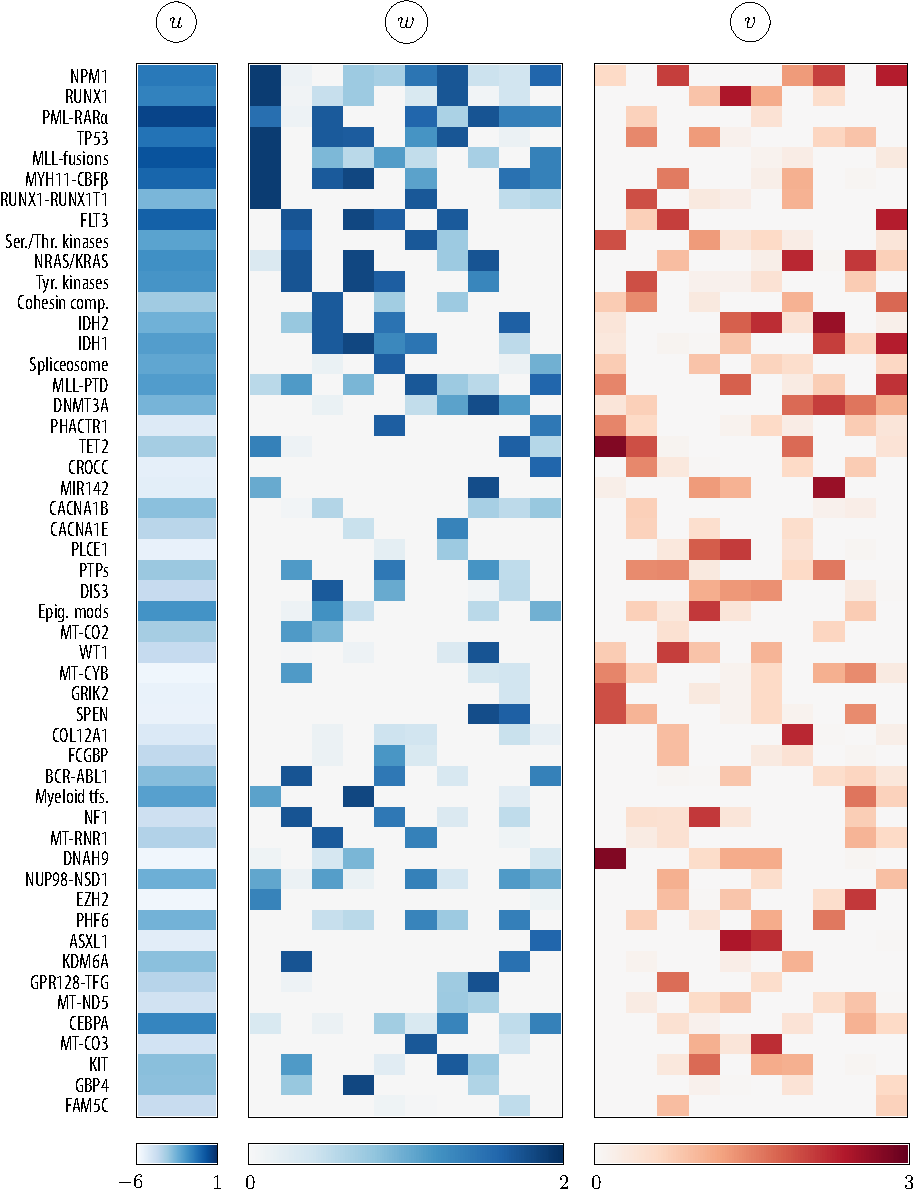
\includegraphics[width=\textwidth]{figures/genes/mat_aml.pdf}\\[2em]
\caption{Test}
\end{figure}

\begin{figure}[htb]
\centering
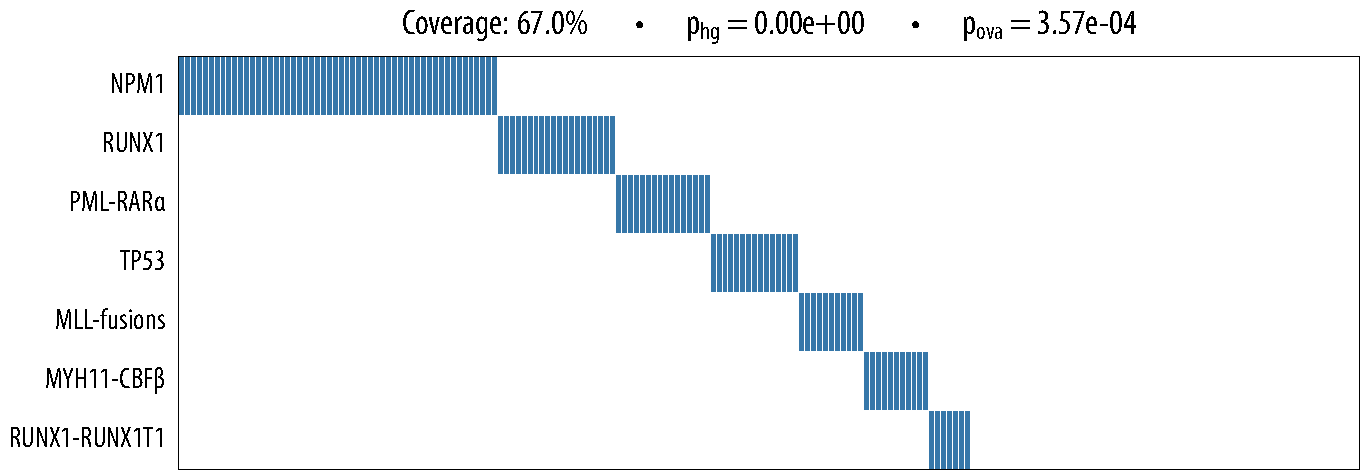
\includegraphics[width=\textwidth]{figures/genes/aml_1.pdf}\\[2em]
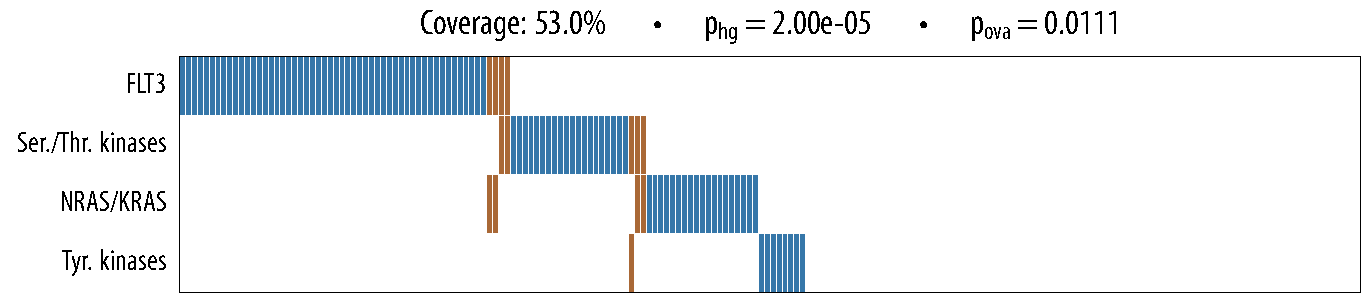
\includegraphics[width=\textwidth]{figures/genes/aml_2.pdf}\\[2em]
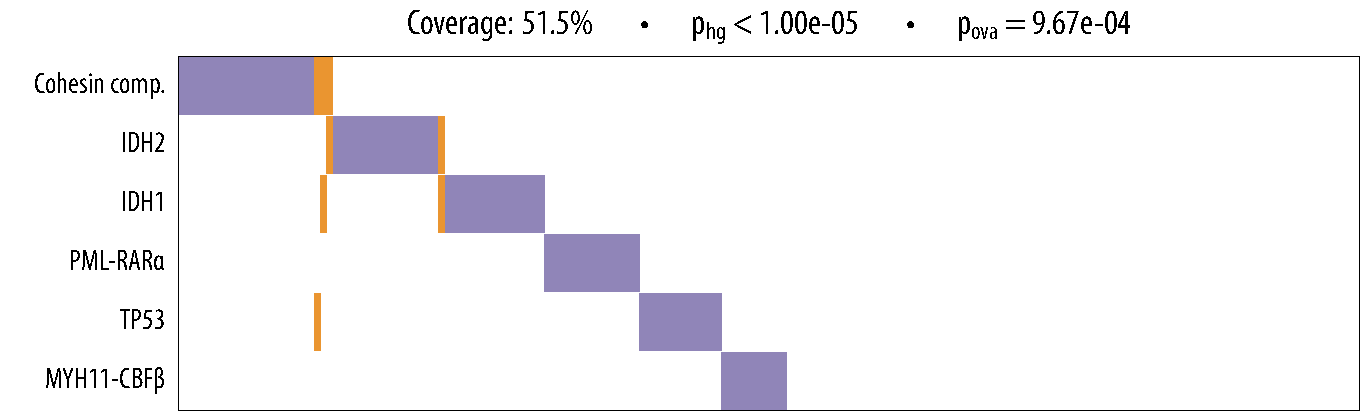
\includegraphics[width=\textwidth]{figures/genes/aml_3.pdf}\\[2em]
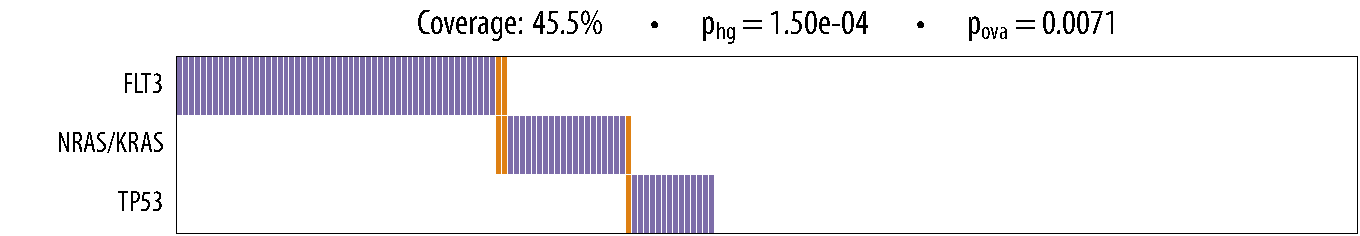
\includegraphics[width=\textwidth]{figures/genes/aml_4.pdf}\\[2em]
\caption{Test}
\end{figure}

\begin{figure}[htb]
\centering
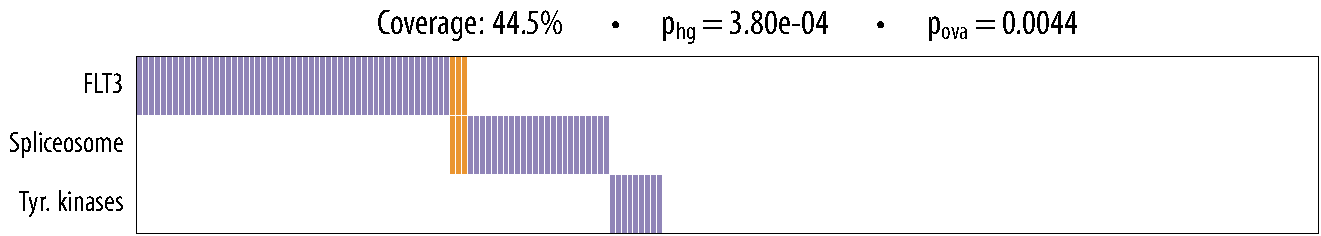
\includegraphics[width=\textwidth]{figures/genes/aml_5.pdf}\\[2em]
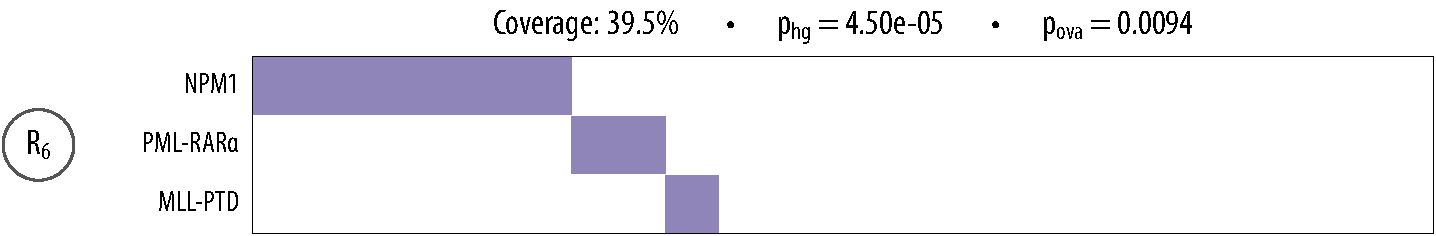
\includegraphics[width=\textwidth]{figures/genes/aml_6.pdf}\\[2em]
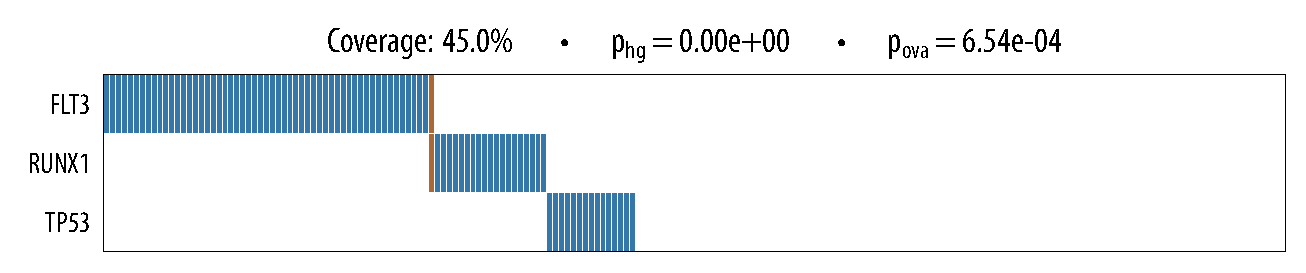
\includegraphics[width=\textwidth]{figures/genes/aml_7.pdf}\\[2em]
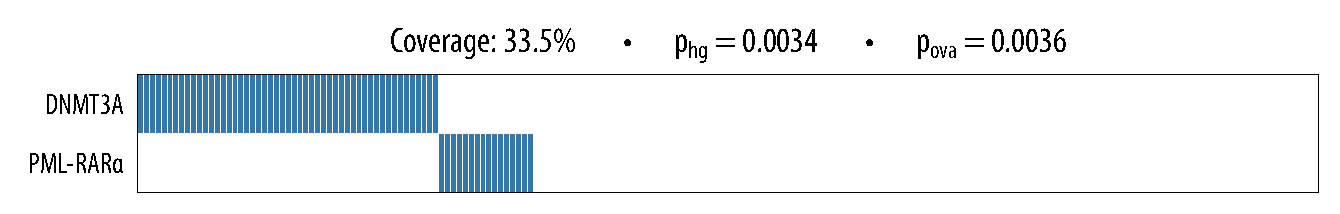
\includegraphics[width=\textwidth]{figures/genes/aml_8.pdf}\\[2em]
\caption{Test}
\end{figure}

\begin{figure}[htb]
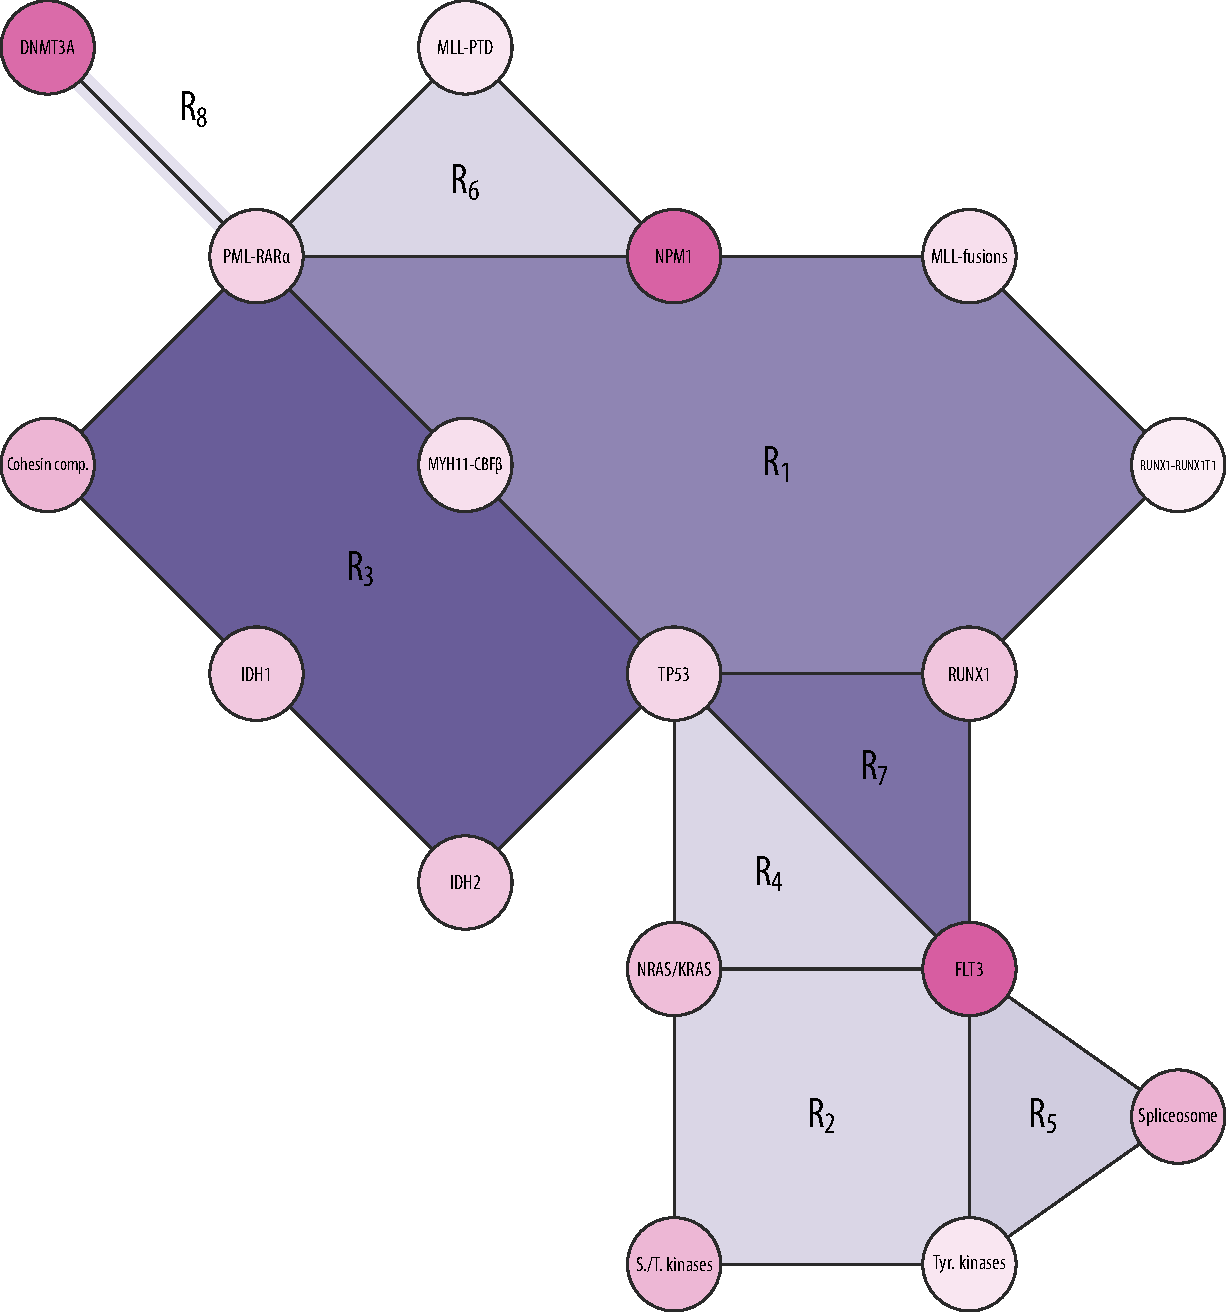
\includegraphics[width=\textwidth]{figures/genes/graph_aml.pdf}\\[2em]
\caption{AML repulsive graph}
\end{figure}

\begin{figure}[htb]
\centering
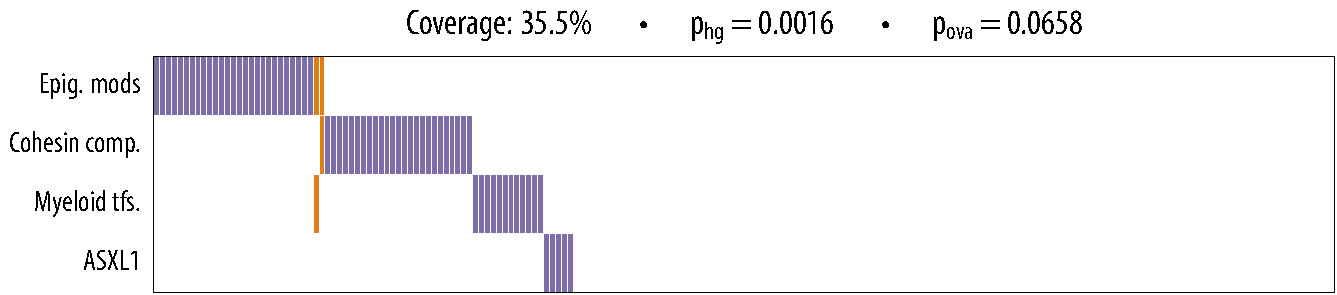
\includegraphics[width=\textwidth]{figures/genes/aml_comet1.pdf}\\[2em]
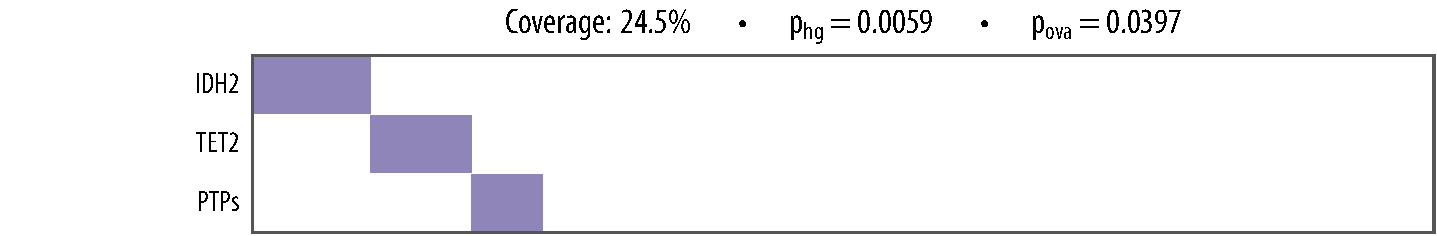
\includegraphics[width=\textwidth]{figures/genes/aml_comet2.pdf}\\[2em]
\caption{CoMEt extra groups (probably appendix)}
\end{figure}

\begin{figure}[htb]
\centering
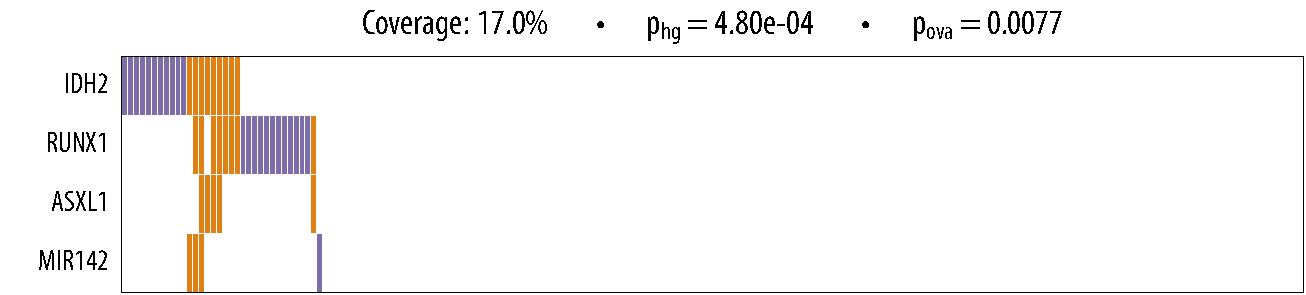
\includegraphics[width=\textwidth]{figures/genes/aml_2_a.pdf}\\[2em]
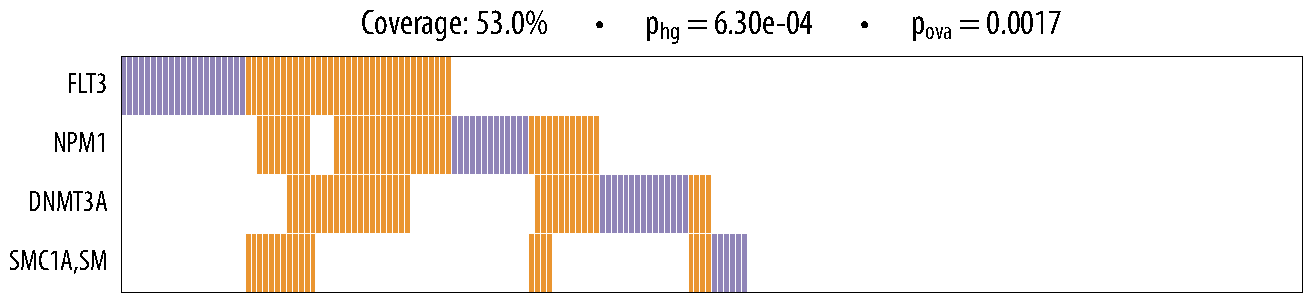
\includegraphics[width=\textwidth]{figures/genes/aml_1_a.pdf}\\[2em]
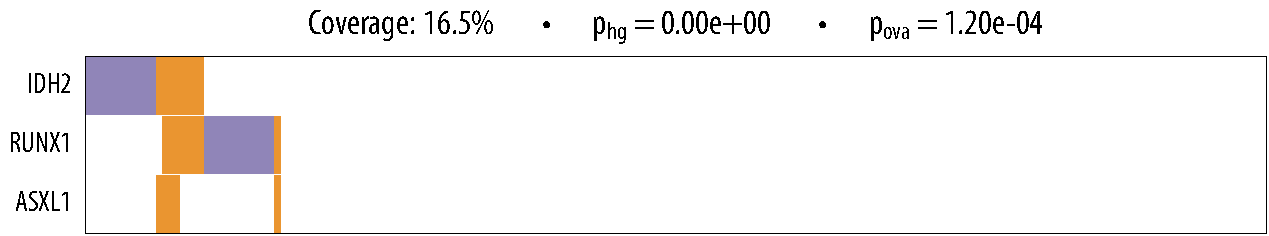
\includegraphics[width=\textwidth]{figures/genes/aml_3_a.pdf}\\[2em]
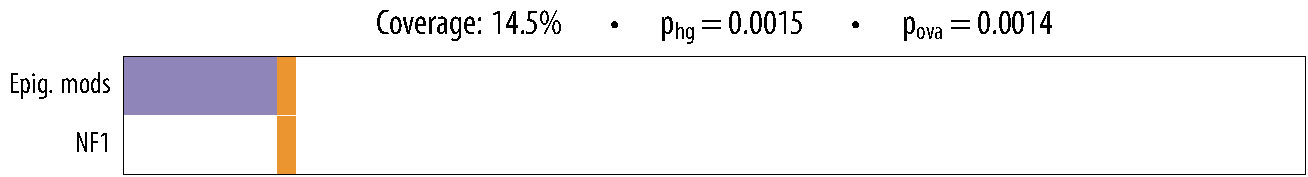
\includegraphics[width=\textwidth]{figures/genes/aml_5_a.pdf}\\[2em]
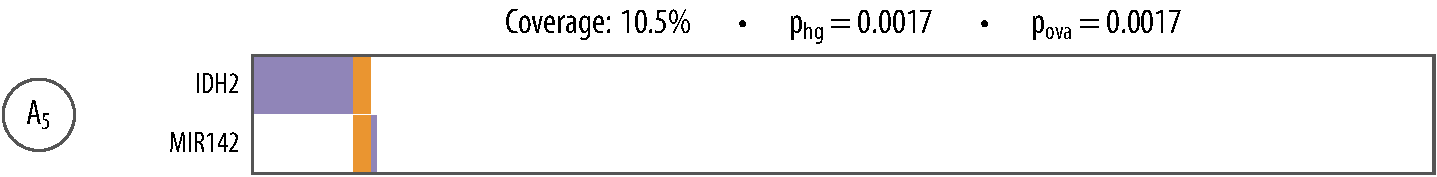
\includegraphics[width=\textwidth]{figures/genes/aml_4_a.pdf}\\[2em]
\caption{Test}
\end{figure}

\subsection{Breast cancer (BRCA)}
\begin{figure}[htb]
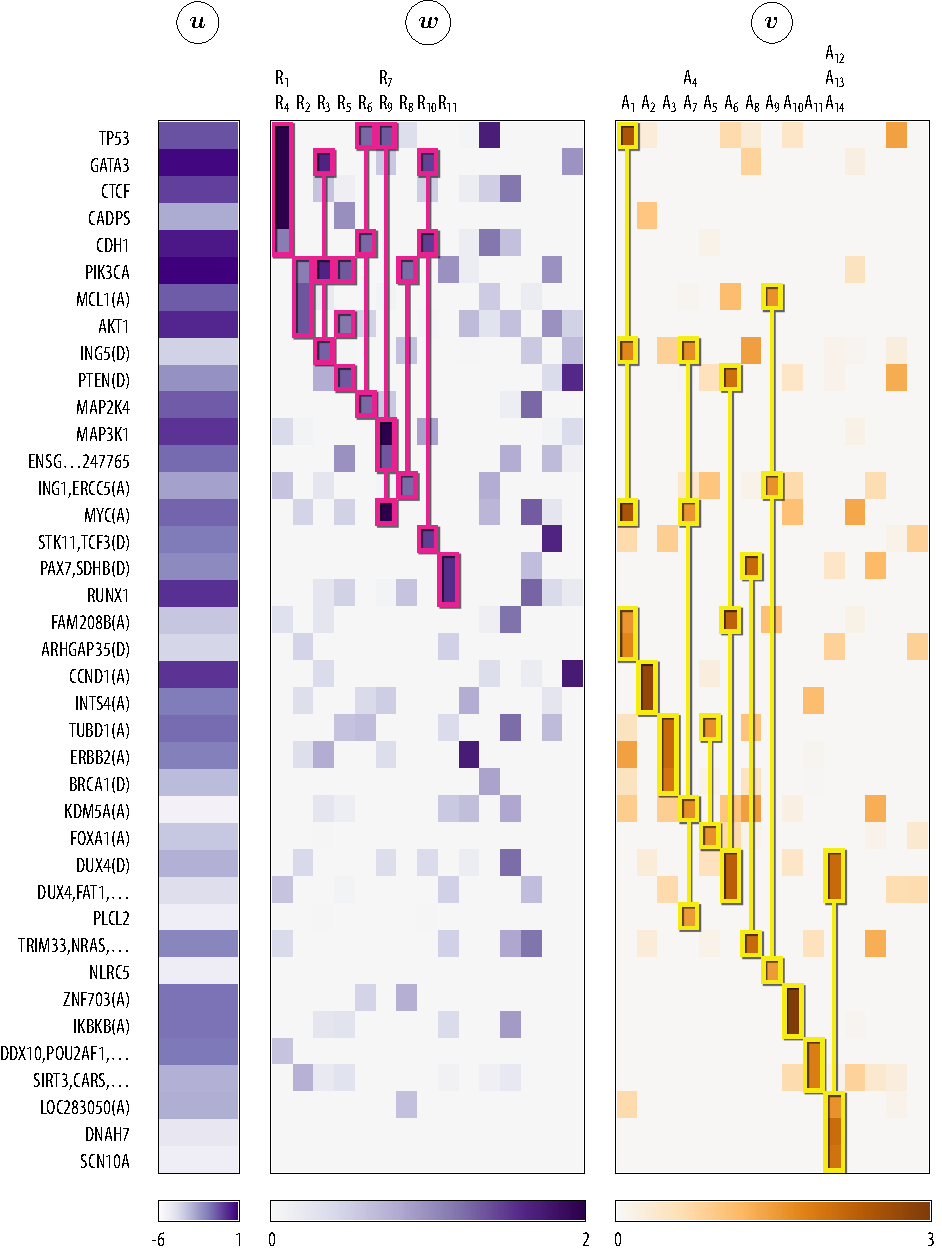
\includegraphics[width=\textwidth]{figures/genes/mat_brca.pdf}\\[2em]
\caption{Test}
\end{figure}

\begin{figure}[htb]
\centering
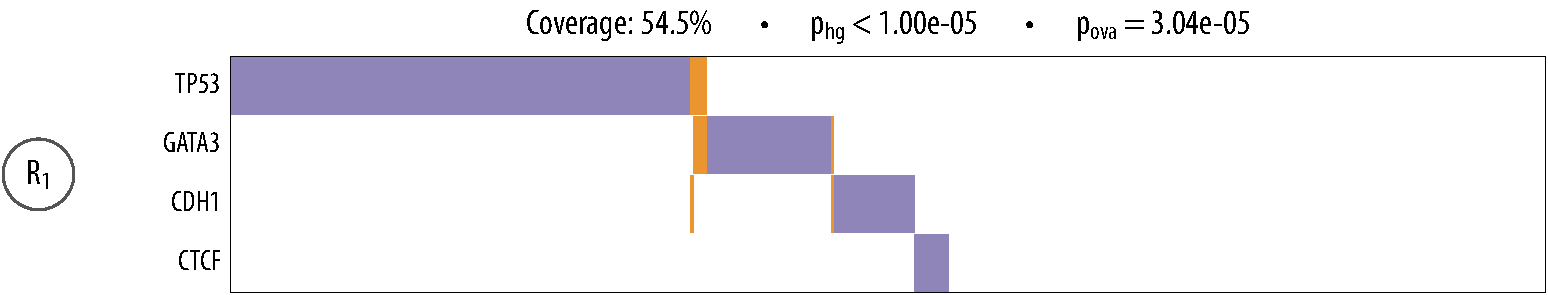
\includegraphics[width=\textwidth]{figures/genes/brca_1.pdf}\\[2em]
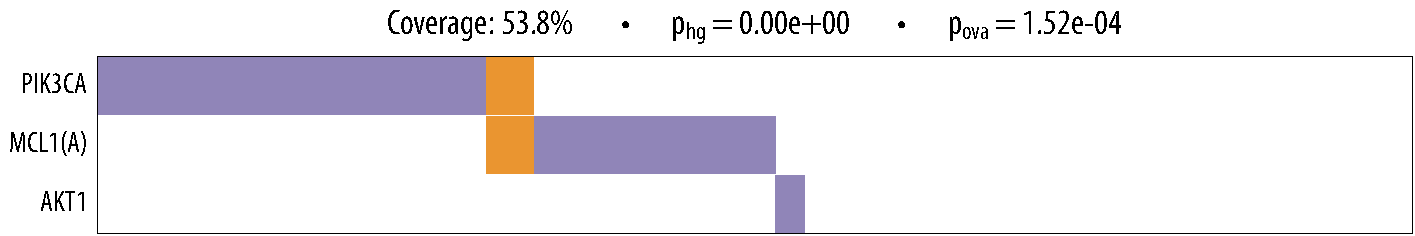
\includegraphics[width=\textwidth]{figures/genes/brca_6.pdf}\\[2em]
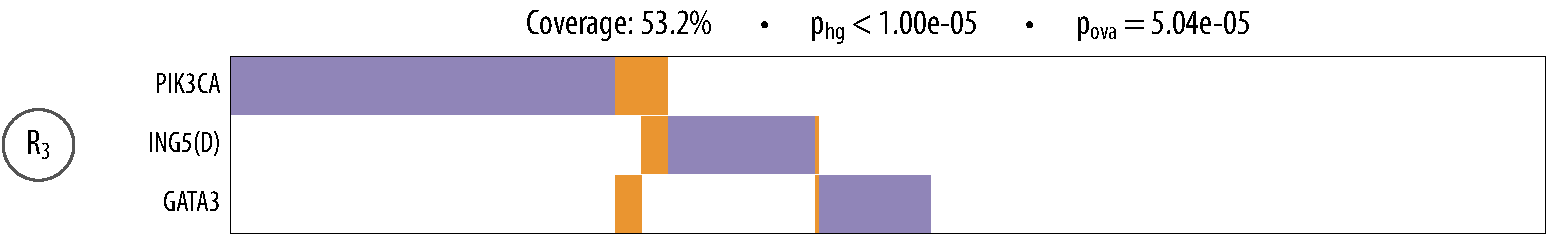
\includegraphics[width=\textwidth]{figures/genes/brca_8.pdf}\\[2em]
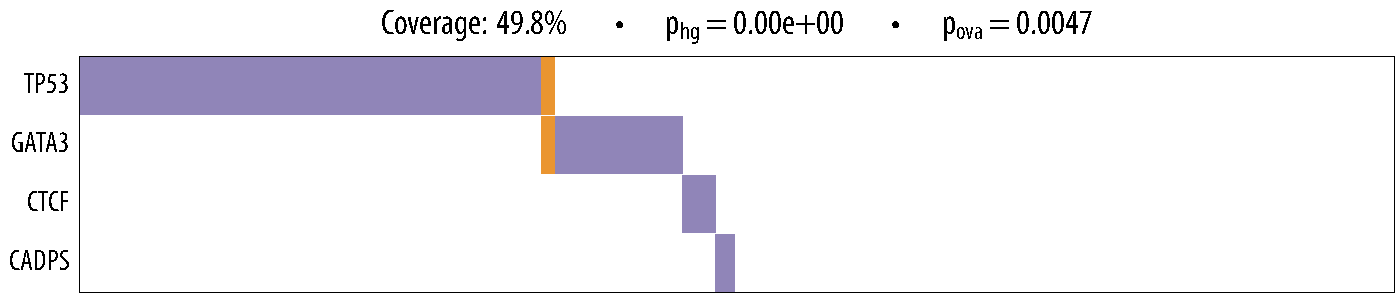
\includegraphics[width=\textwidth]{figures/genes/brca_2.pdf}\\[2em]
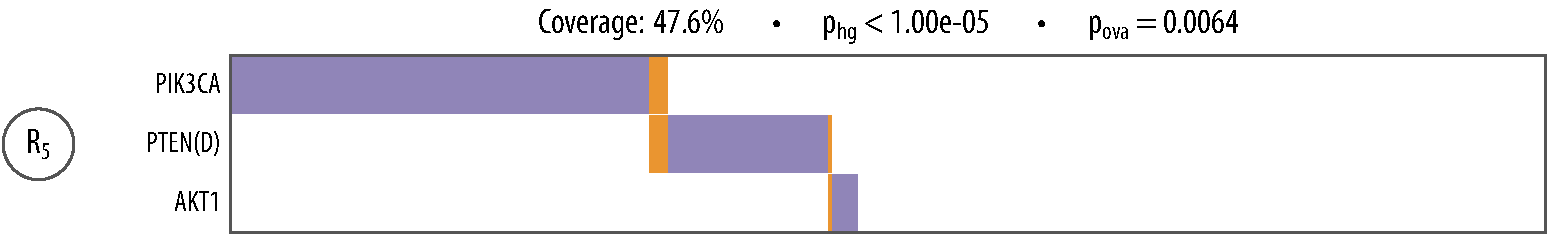
\includegraphics[width=\textwidth]{figures/genes/brca_5.pdf}\\[2em]
\caption{BRCA repulsive (I)}
\end{figure}

\begin{figure}[htb]
\centering
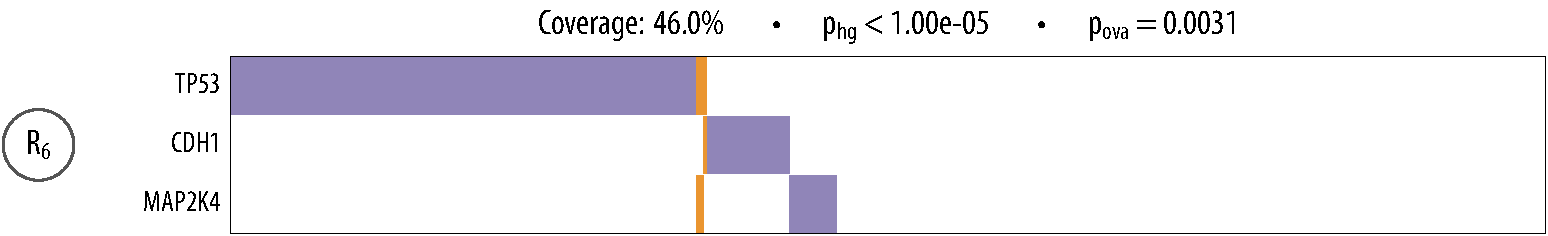
\includegraphics[width=\textwidth]{figures/genes/brca_4.pdf}\\[2em]
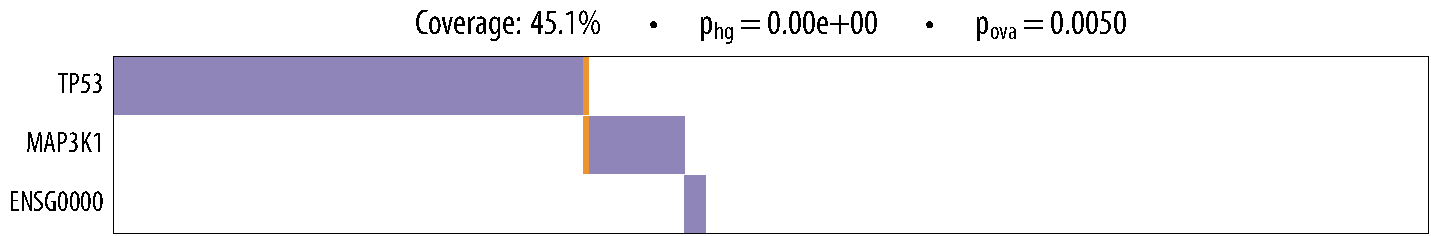
\includegraphics[width=\textwidth]{figures/genes/brca_3.pdf}\\[2em]
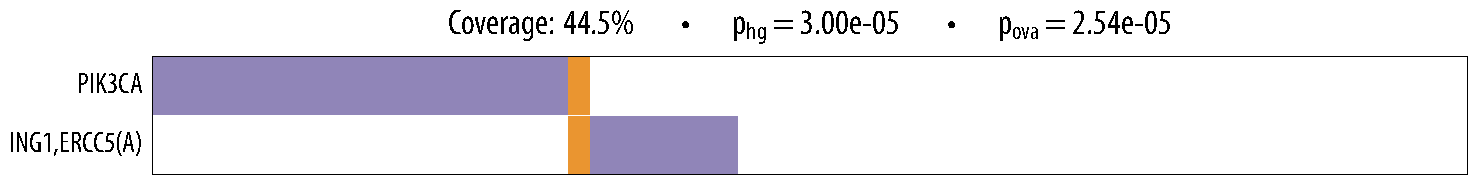
\includegraphics[width=\textwidth]{figures/genes/brca_11.pdf}\\[2em]
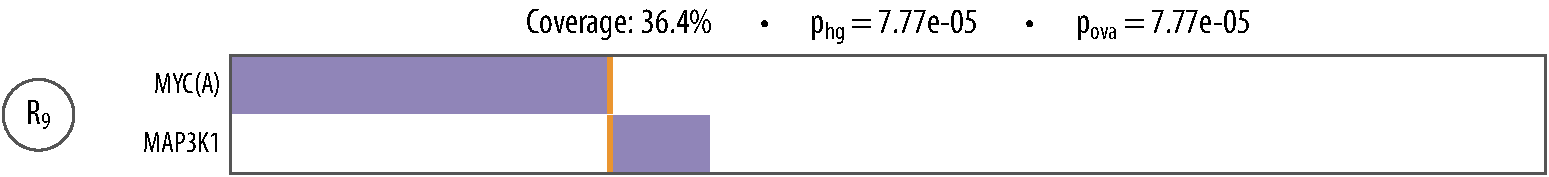
\includegraphics[width=\textwidth]{figures/genes/brca_10.pdf}\\[2em]
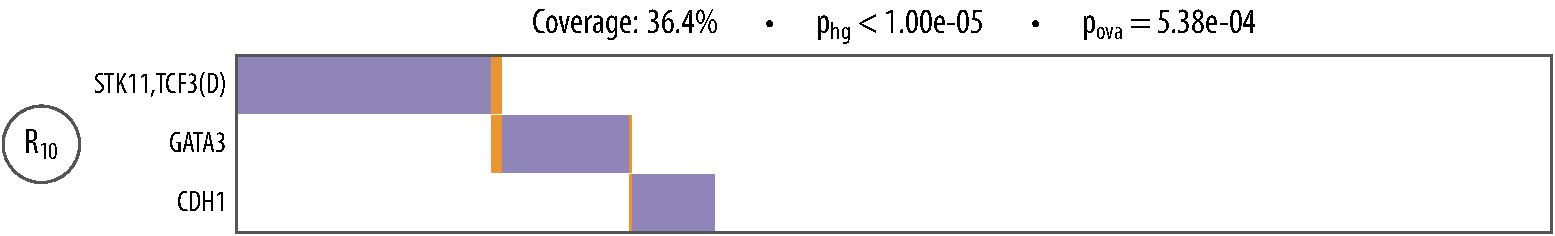
\includegraphics[width=\textwidth]{figures/genes/brca_7.pdf}\\[2em]
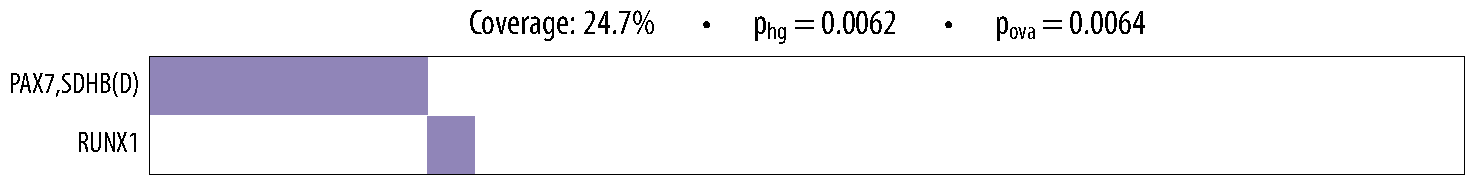
\includegraphics[width=\textwidth]{figures/genes/brca_9.pdf}\\[2em]
\caption{BRCA repulsive (II)}
\end{figure}

\begin{figure}[htb]
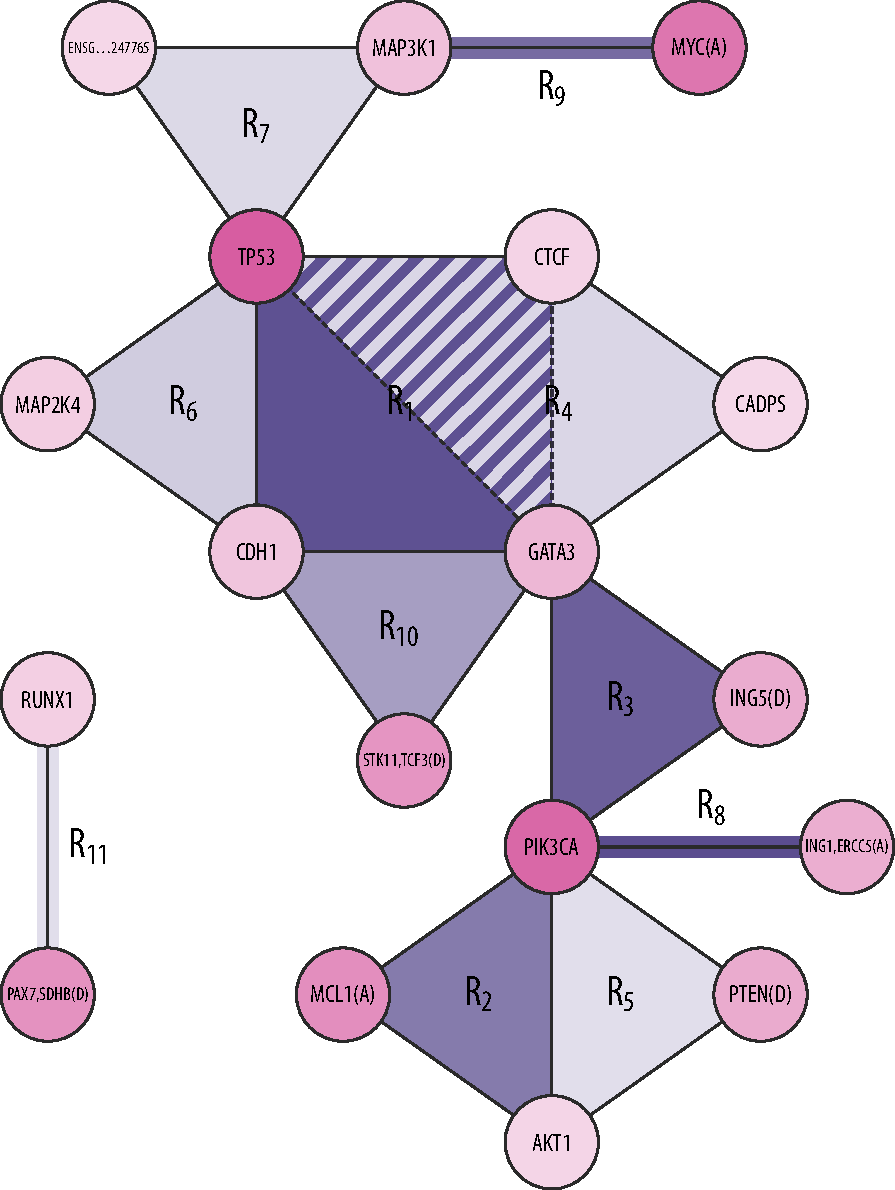
\includegraphics[width=\textwidth]{figures/genes/graph_brca.pdf}\\[2em]
\caption{BRCA repulsive graph}
\end{figure}

\begin{figure}[htb]
\centering
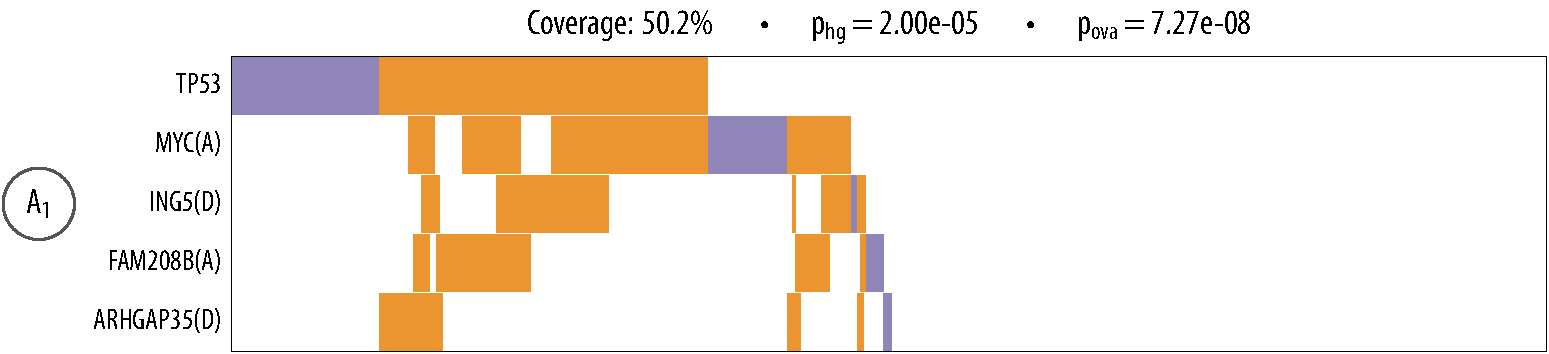
\includegraphics[width=\textwidth]{figures/genes/brca_1_a.pdf}\\[2em]
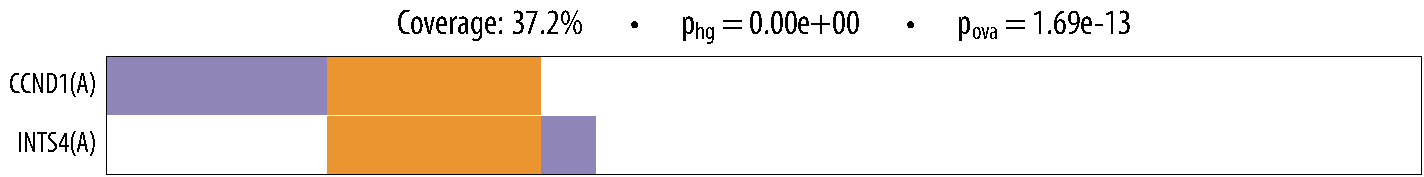
\includegraphics[width=\textwidth]{figures/genes/brca_11_a.pdf}\\[2em]
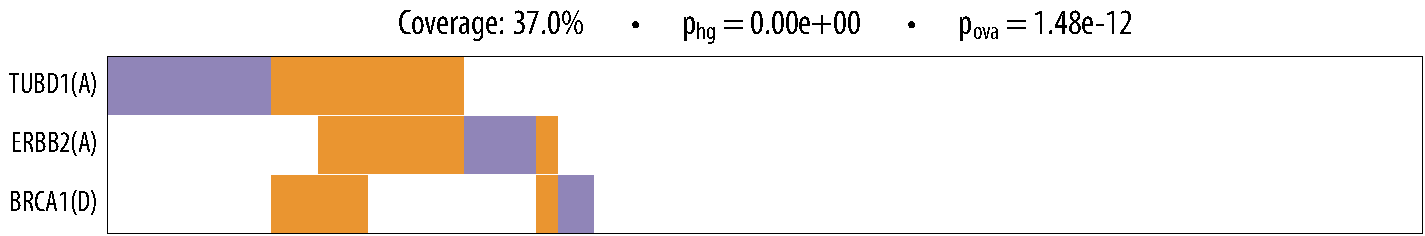
\includegraphics[width=\textwidth]{figures/genes/brca_7_a.pdf}\\[2em]
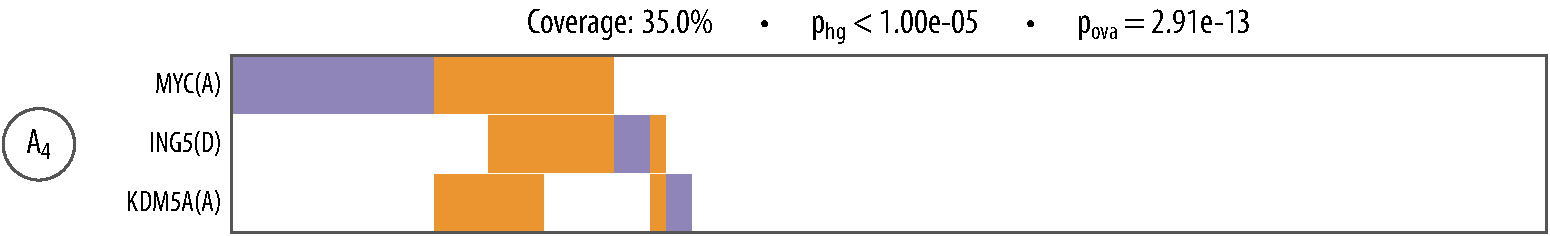
\includegraphics[width=\textwidth]{figures/genes/brca_8_a.pdf}\\[2em]
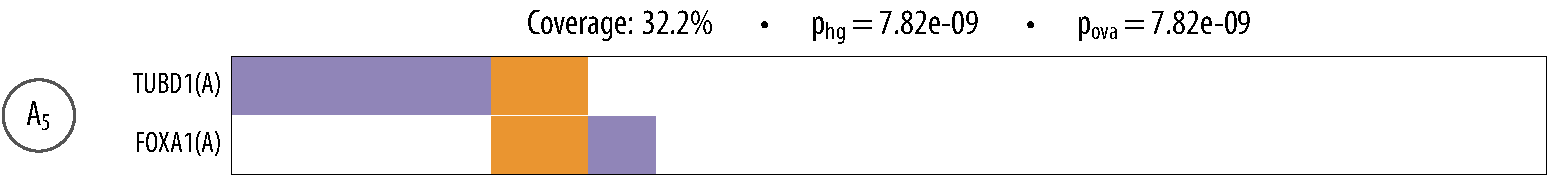
\includegraphics[width=\textwidth]{figures/genes/brca_14_a.pdf}\\[2em]
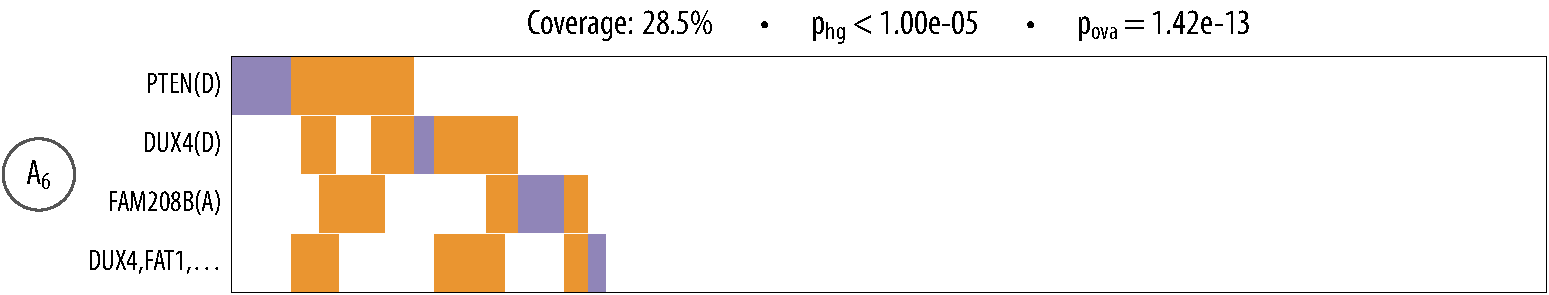
\includegraphics[width=\textwidth]{figures/genes/brca_4_a.pdf}\\[2em]
\caption{BRCA attractive}
\end{figure}

\begin{figure}[htb]
\centering
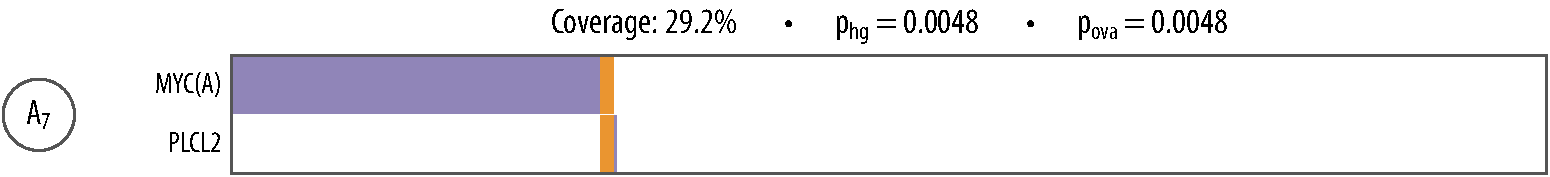
\includegraphics[width=\textwidth]{figures/genes/brca_9_a.pdf}\\[2em]
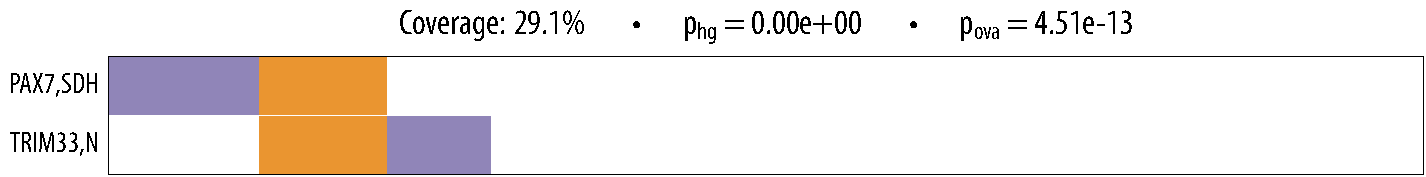
\includegraphics[width=\textwidth]{figures/genes/brca_13_a.pdf}\\[2em]
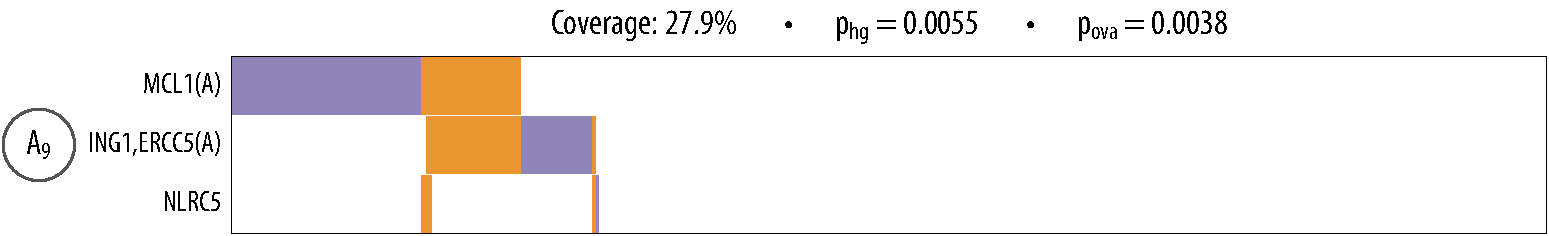
\includegraphics[width=\textwidth]{figures/genes/brca_5_a.pdf}\\[2em]
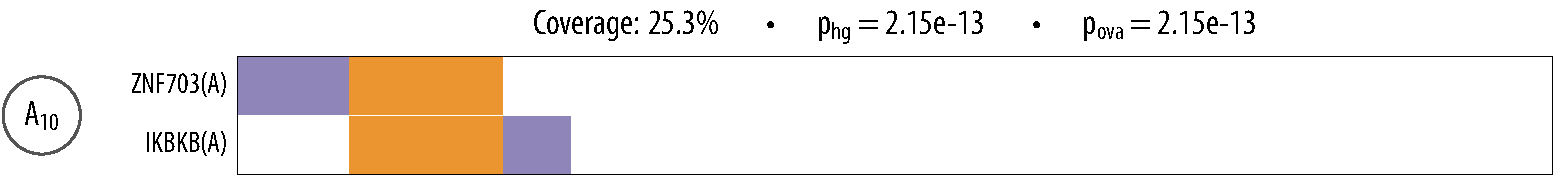
\includegraphics[width=\textwidth]{figures/genes/brca_10_a.pdf}\\[2em]
\includegraphics[width=\textwidth]{figures/genes/brca_12_a.pdf}\\[2em]
\caption{BRCA attractive (appendix I)}
\end{figure}

\begin{figure}[htb]
\centering
\includegraphics[width=\textwidth]{figures/genes/brca_3_a.pdf}\\[2em]
%\includegraphics[width=\textwidth]{figures/genes/brca_15_a.pdf}\\[2em]
\includegraphics[width=\textwidth]{figures/genes/brca_2_a.pdf}\\[2em]
\includegraphics[width=\textwidth]{figures/genes/brca_6_a.pdf}\\[2em]
\caption{BRCA attractive (appendix II)}
\end{figure}

\section{Conclusion}
\chapter{Conclusion} \label{ch:conclusion}

In this thesis, we focused on discrete probabilistic models defined via submodular or supermodular functions, and investigated the use of Markov chain Monte Carlo sampling techniques to perform inference in such models.

We analyzed the mixing behavior of the Gibbs sampler on probabilistic submodular models, and showed that under conditions that quantify the distance from modularity or the influence of element on the function values, we can guarantee polynomial-time or $\mathcal{O}(n\log n)$ mixing, respectively.
These conditions also showed how sub- or supermodularity can lead to improved mixing bounds.

We then proposed a novel sampling procedure that combines the Gibbs sampler with a Metropolis chain that performs global moves to avoid state-space bottlenecks.
The construction of this chain involved creating a mixture of semigradient-based log-modular distributions, and illustrated how concepts from discrete optimization may be leveraged in probabilistic inference.

Finally, we showed how we can use sampling to approximate the likelihood gradients, and perform an approximate likelihood maximization using gradient ascent.
We applied this learning procedure to the problem of modeling interactions of genetic mutations in cancer patients, in particular mutual exclusivity and co-occurrence.
Our results illustrated that our probabilistic framework provides a flexible way to encode such interactions without the need to specify the number or size of the groups that are being searched for.
Moreover, in real cancer data we discovered significant groups of mutations that previous state-of-the-art methods failed to find.

\section{Future Work}
We list here a few promising directions for future work related to this thesis.

\paragraph{Learning models with efficiency guarantees.}
Our approach in \chapref{ch:gibbs} was to provide conditions for efficient sampling in general probabilistic submodular models.
On the other hand, our learning procedure of \chapref{ch:genes} cannot guarantee that these conditions will hold in the resulting model.
It is interesting to consider the problem of directly incorporating conditions for guaranteed inference efficiency into the learning process, in order to make sure that the learned models are amenable to inference.
There has been little work in this direction for a limited model class \citep{domke15}.

\paragraph{Continuous sampling for discrete inference.}
Sampling methods for continuous domains, such as Hamiltonian Monte Carlo, have received increasing attention in the past few years, for their ability to combine gradient information with random momentum to perform more efficient moves in the state space.
There has been some promising recent work on embedding discrete models into suitable continuous domains, then using a continuous sampler, and finally converting the samples back to the discrete domain \citep{zhang12,pakman13,dinh17,nishimura18}.
It is also interesting to investigate whether it is possible to directly define discrete counterparts of momentum and gradients, and, as a result, a discrete version of Hamiltonian Monte Carlo.

\paragraph{Strongly Rayleigh distributions.}
Strongly Rayleigh \citep{borcea08} distributions capture a strong notion of negative dependence between elements, and have been shown to allow for efficient sampling \citep{anari16,li16}.
Except for determinantal point processes, only very few interesting classes of parametric distributions are known to be strongly Rayleigh \citep{li17}.
It is interesting to investigate under what conditions some well-known model classes are strongly Rayleigh, and to find efficient ways to represent and learn more general strongly Rayleigh models.
\appendix
\chapter{Additional Experimental Results}
\vspace{-2em}
\section{Results from \chapref{ch:m3}}
\vspace{-2em}

\setlength\figureheight{0.37\textwidth}
\setlength\figurewidth{0.55\textwidth}
\renewcommand{\subflen}{1.0\textwidth}
\begin{figure}[h!]
  \captionsetup[subfigure]{oneside,margin={2em,0em}}
  \begin{subfigure}[b]{\subflen}
    \centering
    \begin{tikzpicture}


\begin{axis}[%
tick label style={/pgf/number format/fixed,font=\sffamily\small},
label style={font=\sffamily\small},
legend style={font=\sffamily\small},
view={0}{90},
width=\figurewidth,
height=\figureheight,
xmin=0, xmax=200,
xtick={0, 100, 200},
xticklabels={0, 100, 200},
scaled x ticks=false,
xlabel={Time (ms)},
xlabel shift=0em,
ymin=1, ymax=1.52,
ytick={1, 1.5},
yticklabels={1, 1.5},
ylabel={PSRF},
ylabel shift=-1em,
major tick length=2pt,
axis lines*=left,
legend cell align=left,
clip marker paths=true,
legend style={anchor=north east,at={(1,1)},draw=none,row sep=0em},
every axis plot/.append style={
  line width=1.5pt,
  opacity=0.8,
}
]

\addplot [
color=col1dark,
densely dashed,
]
coordinates{
(8.110889,3.597939) +- (-0.282843,0.282843)(9.124750,3.040631) +- (-0.197440,0.197440)(10.138612,2.691309) +- (-0.160233,0.160233)(11.152473,2.554452) +- (-0.165238,0.165238)(12.166334,2.413226) +- (-0.160241,0.160241)(13.180195,2.330296) +- (-0.148466,0.148466)(14.194056,2.215460) +- (-0.130796,0.130796)(15.207917,2.169512) +- (-0.130263,0.130263)(16.221778,2.082272) +- (-0.130343,0.130343)(17.235640,2.028475) +- (-0.144012,0.144012)(18.249501,2.014070) +- (-0.189635,0.189635)(19.263362,2.059465) +- (-0.282843,0.282843)(20.277223,1.948577) +- (-0.207447,0.207447)(21.291084,1.888214) +- (-0.187895,0.187895)(22.304945,1.800753) +- (-0.146235,0.146235)(23.318807,1.749965) +- (-0.125414,0.125414)(24.332668,1.717381) +- (-0.149604,0.149604)(25.346529,1.704961) +- (-0.179373,0.179373)(26.360390,1.685182) +- (-0.188536,0.188536)(27.374251,1.651440) +- (-0.194696,0.194696)(28.388112,1.565033) +- (-0.110935,0.110935)(29.401973,1.494971) +- (-0.060617,0.060617)(30.415835,1.448536) +- (-0.037580,0.037580)(31.429696,1.423904) +- (-0.030389,0.030389)(32.443557,1.404557) +- (-0.025724,0.025724)(33.457418,1.388615) +- (-0.024165,0.024165)(34.471279,1.375496) +- (-0.022723,0.022723)(35.485140,1.365812) +- (-0.022431,0.022431)(36.499002,1.359307) +- (-0.022667,0.022667)(37.512863,1.357107) +- (-0.023374,0.023374)(38.526724,1.353670) +- (-0.024974,0.024974)(39.540585,1.349603) +- (-0.026614,0.026614)(40.554446,1.341914) +- (-0.026115,0.026115)(40.554446,1.341914) +- (-0.026115,0.026115)(42.582168,1.327010) +- (-0.025499,0.025499)(44.609891,1.309038) +- (-0.022776,0.022776)(46.637613,1.291903) +- (-0.021510,0.021510)(48.665335,1.276404) +- (-0.019627,0.019627)(50.693058,1.265232) +- (-0.019791,0.019791)(52.720780,1.257915) +- (-0.022160,0.022160)(54.748502,1.245602) +- (-0.022382,0.022382)(56.776225,1.229363) +- (-0.019007,0.019007)(58.803947,1.212160) +- (-0.014853,0.014853)(60.831669,1.202877) +- (-0.014921,0.014921)(62.859391,1.194305) +- (-0.016019,0.016019)(64.887114,1.187061) +- (-0.016566,0.016566)(66.914836,1.181264) +- (-0.015779,0.015779)(68.942558,1.176979) +- (-0.015684,0.015684)(70.970281,1.173301) +- (-0.016778,0.016778)(72.998003,1.166561) +- (-0.015625,0.015625)(75.025725,1.160849) +- (-0.014327,0.014327)(77.053448,1.157492) +- (-0.013240,0.013240)(79.081170,1.152301) +- (-0.012648,0.012648)(81.108892,1.146251) +- (-0.010389,0.010389)(83.136615,1.142146) +- (-0.008755,0.008755)(85.164337,1.138389) +- (-0.008279,0.008279)(87.192059,1.134830) +- (-0.007781,0.007781)(89.219781,1.131334) +- (-0.007385,0.007385)(91.247504,1.129364) +- (-0.007120,0.007120)(93.275226,1.127263) +- (-0.007972,0.007972)(95.302948,1.124395) +- (-0.008520,0.008520)(97.330671,1.119219) +- (-0.008856,0.008856)(99.358393,1.117366) +- (-0.010033,0.010033)(101.386115,1.114105) +- (-0.008819,0.008819)(103.413838,1.113725) +- (-0.008468,0.008468)(105.441560,1.111648) +- (-0.008166,0.008166)(107.469282,1.109619) +- (-0.007836,0.007836)(109.497005,1.107001) +- (-0.007309,0.007309)(111.524727,1.104818) +- (-0.006968,0.006968)(113.552449,1.104075) +- (-0.006324,0.006324)(115.580171,1.102976) +- (-0.006398,0.006398)(117.607894,1.100722) +- (-0.006288,0.006288)(119.635616,1.097873) +- (-0.005578,0.005578)(121.663338,1.095111) +- (-0.005033,0.005033)(123.691061,1.093478) +- (-0.005158,0.005158)(125.718783,1.091610) +- (-0.005177,0.005177)(127.746505,1.090405) +- (-0.005001,0.005001)(129.774228,1.089527) +- (-0.004982,0.004982)(131.801950,1.088855) +- (-0.004821,0.004821)(133.829672,1.087810) +- (-0.004819,0.004819)(135.857395,1.086178) +- (-0.004890,0.004890)(137.885117,1.083872) +- (-0.004823,0.004823)(139.912839,1.082651) +- (-0.004757,0.004757)(141.940561,1.082000) +- (-0.004411,0.004411)(143.968284,1.081654) +- (-0.004404,0.004404)(145.996006,1.080664) +- (-0.004261,0.004261)(148.023728,1.079681) +- (-0.004000,0.004000)(150.051451,1.078145) +- (-0.004157,0.004157)(152.079173,1.077135) +- (-0.004285,0.004285)(154.106895,1.076356) +- (-0.004383,0.004383)(156.134618,1.075704) +- (-0.004286,0.004286)(158.162340,1.074393) +- (-0.004038,0.004038)(160.190062,1.072686) +- (-0.003808,0.003808)(162.217785,1.071898) +- (-0.003671,0.003671)(164.245507,1.070577) +- (-0.003569,0.003569)(166.273229,1.068997) +- (-0.003373,0.003373)(168.300951,1.067786) +- (-0.003359,0.003359)(170.328674,1.067305) +- (-0.003437,0.003437)(172.356396,1.066197) +- (-0.003413,0.003413)(174.384118,1.064406) +- (-0.003289,0.003289)(176.411841,1.062878) +- (-0.003119,0.003119)(178.439563,1.061796) +- (-0.003118,0.003118)(180.467285,1.061438) +- (-0.003328,0.003328)(182.495008,1.061019) +- (-0.003352,0.003352)(184.522730,1.060327) +- (-0.003275,0.003275)(186.550452,1.059904) +- (-0.003248,0.003248)(188.578174,1.059435) +- (-0.003126,0.003126)(190.605897,1.058691) +- (-0.002941,0.002941)(192.633619,1.057888) +- (-0.002763,0.002763)(194.661341,1.057200) +- (-0.002759,0.002759)(196.689064,1.056826) +- (-0.002693,0.002693)(198.716786,1.056174) +- (-0.002721,0.002721)(200.744508,1.055308) +- (-0.002654,0.002654)(202.772231,1.054398) +- (-0.002602,0.002602)
};
\addlegendentry{\textsc{Gibbs}}


\addplot [
color=col2
]
coordinates{
(4.691006,2.314380) +- (-0.145936,0.145936)(5.863757,2.004462) +- (-0.127423,0.127423)(7.036509,1.793518) +- (-0.080239,0.080239)(8.209260,1.631944) +- (-0.067338,0.067338)(9.382012,1.547655) +- (-0.050816,0.050816)(10.554763,1.467467) +- (-0.045281,0.045281)(11.727515,1.434199) +- (-0.047724,0.047724)(12.900266,1.387869) +- (-0.026698,0.026698)(14.073018,1.352802) +- (-0.024894,0.024894)(15.245769,1.325987) +- (-0.022519,0.022519)(16.418521,1.300620) +- (-0.018924,0.018924)(17.591272,1.276801) +- (-0.015945,0.015945)(18.764024,1.258876) +- (-0.015658,0.015658)(19.936775,1.247336) +- (-0.015910,0.015910)(21.109527,1.231760) +- (-0.014686,0.014686)(22.282278,1.220108) +- (-0.014804,0.014804)(23.455030,1.209891) +- (-0.016687,0.016687)(24.627781,1.197965) +- (-0.017494,0.017494)(25.800533,1.187772) +- (-0.017134,0.017134)(26.973284,1.181613) +- (-0.016117,0.016117)(28.146036,1.175375) +- (-0.015438,0.015438)(29.318787,1.167047) +- (-0.014963,0.014963)(30.491539,1.162951) +- (-0.014282,0.014282)(31.664290,1.159416) +- (-0.013639,0.013639)(32.837042,1.151083) +- (-0.012802,0.012802)(34.009793,1.143855) +- (-0.013366,0.013366)(35.182545,1.139644) +- (-0.013836,0.013836)(36.355296,1.136401) +- (-0.012880,0.012880)(37.528048,1.130305) +- (-0.011110,0.011110)(38.700799,1.127232) +- (-0.010790,0.010790)(39.873550,1.121431) +- (-0.010224,0.010224)(41.046302,1.116844) +- (-0.009764,0.009764)(42.219053,1.113843) +- (-0.009180,0.009180)(43.391805,1.109543) +- (-0.008657,0.008657)(44.564556,1.105246) +- (-0.008078,0.008078)(45.737308,1.101941) +- (-0.007431,0.007431)(46.910059,1.097746) +- (-0.006427,0.006427)(46.910059,1.097746) +- (-0.006427,0.006427)(49.255562,1.090858) +- (-0.005703,0.005703)(51.601065,1.085136) +- (-0.004712,0.004712)(53.946568,1.082785) +- (-0.004480,0.004480)(56.292071,1.078993) +- (-0.004481,0.004481)(58.637574,1.075416) +- (-0.004278,0.004278)(60.983077,1.072572) +- (-0.004408,0.004408)(63.328580,1.072164) +- (-0.004253,0.004253)(65.674083,1.071047) +- (-0.003945,0.003945)(68.019586,1.068267) +- (-0.003995,0.003995)(70.365089,1.064680) +- (-0.003782,0.003782)(72.710592,1.062878) +- (-0.003607,0.003607)(75.056095,1.060127) +- (-0.002978,0.002978)(77.401598,1.057291) +- (-0.002852,0.002852)(79.747101,1.056389) +- (-0.002972,0.002972)(82.092604,1.054495) +- (-0.002850,0.002850)(84.438107,1.052421) +- (-0.002805,0.002805)(86.783610,1.052303) +- (-0.003047,0.003047)(89.129113,1.051432) +- (-0.002882,0.002882)(91.474616,1.049071) +- (-0.002860,0.002860)(93.820119,1.048121) +- (-0.002986,0.002986)(96.165622,1.046968) +- (-0.002974,0.002974)(98.511125,1.046242) +- (-0.002929,0.002929)(100.856628,1.046152) +- (-0.002783,0.002783)(103.202131,1.045838) +- (-0.002628,0.002628)(105.547634,1.044434) +- (-0.002501,0.002501)(107.893137,1.043060) +- (-0.002611,0.002611)(110.238640,1.042289) +- (-0.002473,0.002473)(112.584143,1.041161) +- (-0.002194,0.002194)(114.929646,1.040078) +- (-0.002039,0.002039)(117.275149,1.038894) +- (-0.001963,0.001963)(119.620651,1.037761) +- (-0.002019,0.002019)(121.966154,1.036455) +- (-0.001902,0.001902)(124.311657,1.035295) +- (-0.001652,0.001652)(126.657160,1.034810) +- (-0.001550,0.001550)(129.002663,1.034331) +- (-0.001533,0.001533)(131.348166,1.033830) +- (-0.001393,0.001393)(133.693669,1.032976) +- (-0.001362,0.001362)(136.039172,1.032553) +- (-0.001368,0.001368)(138.384675,1.031991) +- (-0.001444,0.001444)(140.730178,1.031694) +- (-0.001432,0.001432)(143.075681,1.031078) +- (-0.001410,0.001410)(145.421184,1.030946) +- (-0.001536,0.001536)(147.766687,1.030691) +- (-0.001492,0.001492)(150.112190,1.030606) +- (-0.001415,0.001415)(152.457693,1.030274) +- (-0.001521,0.001521)(154.803196,1.029901) +- (-0.001567,0.001567)(157.148699,1.029501) +- (-0.001596,0.001596)(159.494202,1.029197) +- (-0.001490,0.001490)(161.839705,1.028674) +- (-0.001432,0.001432)(164.185208,1.028292) +- (-0.001420,0.001420)(166.530711,1.027638) +- (-0.001465,0.001465)(168.876214,1.027133) +- (-0.001453,0.001453)(171.221717,1.027022) +- (-0.001433,0.001433)(173.567220,1.026421) +- (-0.001474,0.001474)(175.912723,1.025866) +- (-0.001395,0.001395)(178.258226,1.025313) +- (-0.001397,0.001397)(180.603729,1.025126) +- (-0.001384,0.001384)(182.949232,1.024998) +- (-0.001477,0.001477)(185.294735,1.024660) +- (-0.001446,0.001446)(187.640238,1.024171) +- (-0.001362,0.001362)(189.985741,1.023864) +- (-0.001253,0.001253)(192.331244,1.023532) +- (-0.001167,0.001167)(194.676747,1.023254) +- (-0.001154,0.001154)(197.022249,1.023072) +- (-0.001145,0.001145)(199.367752,1.022695) +- (-0.001132,0.001132)(201.713255,1.022507) +- (-0.001124,0.001124)(204.058758,1.022286) +- (-0.001143,0.001143)(206.404261,1.021894) +- (-0.001132,0.001132)(208.749764,1.021687) +- (-0.001104,0.001104)(211.095267,1.021078) +- (-0.000988,0.000988)(213.440770,1.020705) +- (-0.000968,0.000968)(215.786273,1.020400) +- (-0.000900,0.000900)(218.131776,1.020334) +- (-0.000907,0.000907)(220.477279,1.020393) +- (-0.000906,0.000906)(222.822782,1.020249) +- (-0.000837,0.000837)(225.168285,1.020091) +- (-0.000844,0.000844)(227.513788,1.019827) +- (-0.000798,0.000798)(229.859291,1.019461) +- (-0.000836,0.000836)(232.204794,1.019257) +- (-0.000829,0.000829)(234.550297,1.019229) +- (-0.000875,0.000875)
};
\addlegendentry{\textsc{Combo-R}}


\addplot [
color=col3
]
coordinates{
(2.353020,3.854406) +- (-0.282843,0.282843)(3.529530,2.516837) +- (-0.198273,0.198273)(4.706040,2.080291) +- (-0.204548,0.204548)(5.882550,1.761562) +- (-0.101370,0.101370)(7.059060,1.588895) +- (-0.068315,0.068315)(8.235570,1.530598) +- (-0.077335,0.077335)(9.412080,1.472095) +- (-0.088279,0.088279)(10.588590,1.407313) +- (-0.069317,0.069317)(11.765099,1.328349) +- (-0.050041,0.050041)(12.941609,1.280189) +- (-0.046740,0.046740)(14.118119,1.241093) +- (-0.028634,0.028634)(15.294629,1.225659) +- (-0.018168,0.018168)(16.471139,1.214143) +- (-0.016083,0.016083)(17.647649,1.199464) +- (-0.015557,0.015557)(18.824159,1.192993) +- (-0.017602,0.017602)(20.000669,1.182354) +- (-0.016598,0.016598)(21.177179,1.173964) +- (-0.016687,0.016687)(22.353689,1.162564) +- (-0.013994,0.013994)(23.530199,1.153207) +- (-0.012485,0.012485)(24.706709,1.146027) +- (-0.011376,0.011376)(25.883219,1.138410) +- (-0.011042,0.011042)(27.059729,1.132240) +- (-0.010125,0.010125)(28.236239,1.124508) +- (-0.009295,0.009295)(29.412749,1.120885) +- (-0.010133,0.010133)(30.589259,1.114675) +- (-0.009175,0.009175)(31.765769,1.110488) +- (-0.008958,0.008958)(32.942279,1.106881) +- (-0.007907,0.007907)(34.118789,1.104418) +- (-0.007560,0.007560)(35.295298,1.099178) +- (-0.007433,0.007433)(36.471808,1.094869) +- (-0.007824,0.007824)(37.648318,1.092353) +- (-0.007203,0.007203)(38.824828,1.089835) +- (-0.006443,0.006443)(40.001338,1.086294) +- (-0.005841,0.005841)(41.177848,1.083016) +- (-0.004871,0.004871)(42.354358,1.080625) +- (-0.004230,0.004230)(43.530868,1.078600) +- (-0.003971,0.003971)(44.707378,1.075129) +- (-0.003631,0.003631)(45.883888,1.073524) +- (-0.003559,0.003559)(47.060398,1.071891) +- (-0.003385,0.003385)(47.060398,1.071891) +- (-0.003385,0.003385)(49.413418,1.066995) +- (-0.003261,0.003261)(51.766438,1.064854) +- (-0.003031,0.003031)(54.119458,1.062135) +- (-0.003158,0.003158)(56.472478,1.060072) +- (-0.002924,0.002924)(58.825497,1.058380) +- (-0.002652,0.002652)(61.178517,1.055289) +- (-0.003135,0.003135)(63.531537,1.053504) +- (-0.002473,0.002473)(65.884557,1.051133) +- (-0.002215,0.002215)(68.237577,1.049357) +- (-0.002129,0.002129)(70.590597,1.048042) +- (-0.002443,0.002443)(72.943617,1.046165) +- (-0.002292,0.002292)(75.296637,1.044985) +- (-0.002335,0.002335)(77.649657,1.043813) +- (-0.002302,0.002302)(80.002677,1.042142) +- (-0.002126,0.002126)(82.355696,1.040972) +- (-0.001732,0.001732)(84.708716,1.038792) +- (-0.001605,0.001605)(87.061736,1.037901) +- (-0.001482,0.001482)(89.414756,1.037031) +- (-0.001745,0.001745)(91.767776,1.036926) +- (-0.002238,0.002238)(94.120796,1.036016) +- (-0.002091,0.002091)(96.473816,1.034859) +- (-0.002239,0.002239)(98.826836,1.033716) +- (-0.002164,0.002164)(101.179856,1.032822) +- (-0.001992,0.001992)(103.532876,1.031838) +- (-0.001809,0.001809)(105.885895,1.030816) +- (-0.001774,0.001774)(108.238915,1.030378) +- (-0.001692,0.001692)(110.591935,1.030052) +- (-0.001777,0.001777)(112.944955,1.029630) +- (-0.001723,0.001723)(115.297975,1.028859) +- (-0.001648,0.001648)(117.650995,1.028342) +- (-0.001664,0.001664)(120.004015,1.027460) +- (-0.001711,0.001711)(122.357035,1.026793) +- (-0.001637,0.001637)(124.710055,1.026026) +- (-0.001552,0.001552)(127.063074,1.025250) +- (-0.001265,0.001265)(129.416094,1.025001) +- (-0.001289,0.001289)(131.769114,1.024221) +- (-0.001330,0.001330)(134.122134,1.023217) +- (-0.001235,0.001235)(136.475154,1.023087) +- (-0.001262,0.001262)(138.828174,1.022697) +- (-0.001187,0.001187)(141.181194,1.022573) +- (-0.001180,0.001180)(143.534214,1.022419) +- (-0.001269,0.001269)(145.887234,1.022147) +- (-0.001212,0.001212)(148.240254,1.021630) +- (-0.001206,0.001206)(150.593273,1.021636) +- (-0.001243,0.001243)(152.946293,1.021386) +- (-0.001207,0.001207)(155.299313,1.021237) +- (-0.001212,0.001212)(157.652333,1.020897) +- (-0.001196,0.001196)(160.005353,1.020573) +- (-0.001154,0.001154)(162.358373,1.020276) +- (-0.001089,0.001089)(164.711393,1.019911) +- (-0.001184,0.001184)(167.064413,1.019570) +- (-0.001224,0.001224)(169.417433,1.019220) +- (-0.001139,0.001139)(171.770453,1.018847) +- (-0.001054,0.001054)(174.123472,1.018390) +- (-0.000911,0.000911)(176.476492,1.018087) +- (-0.000910,0.000910)(178.829512,1.018215) +- (-0.001009,0.001009)(181.182532,1.017975) +- (-0.000981,0.000981)(183.535552,1.017773) +- (-0.000918,0.000918)(185.888572,1.017623) +- (-0.000880,0.000880)(188.241592,1.017201) +- (-0.000808,0.000808)(190.594612,1.017108) +- (-0.000833,0.000833)(192.947632,1.016947) +- (-0.000744,0.000744)(195.300652,1.016976) +- (-0.000757,0.000757)(197.653671,1.016918) +- (-0.000846,0.000846)(200.006691,1.016655) +- (-0.000857,0.000857)(202.359711,1.016267) +- (-0.000828,0.000828)(204.712731,1.016105) +- (-0.000774,0.000774)(207.065751,1.015787) +- (-0.000799,0.000799)(209.418771,1.015690) +- (-0.000837,0.000837)(211.771791,1.015584) +- (-0.000785,0.000785)(214.124811,1.015477) +- (-0.000837,0.000837)(216.477831,1.015410) +- (-0.000880,0.000880)(218.830851,1.015213) +- (-0.000865,0.000865)(221.183870,1.014935) +- (-0.000832,0.000832)(223.536890,1.014694) +- (-0.000838,0.000838)(225.889910,1.014629) +- (-0.000778,0.000778)(228.242930,1.014533) +- (-0.000751,0.000751)(230.595950,1.014393) +- (-0.000742,0.000742)(232.948970,1.014260) +- (-0.000782,0.000782)(235.301990,1.014056) +- (-0.000720,0.000720)
};
\addlegendentry{\textsc{Combo-I}}

\end{axis}
\end{tikzpicture}

    \vspace{-0.5em}
    \caption{\textsc{Water}}
    \label{fig:water1_time}
  \end{subfigure}\\
  \begin{subfigure}[b]{\subflen}
    \centering
    \begin{tikzpicture}


\begin{axis}[%
tick label style={/pgf/number format/fixed,font=\sffamily\small},
label style={font=\sffamily\small},
legend style={font=\sffamily\small},
view={0}{90},
width=\figurewidth,
height=\figureheight,
xmin=0, xmax=300,
xtick={0, 100, 200, 300},
xticklabels={0, 100, 200, 300},
scaled x ticks=false,
xlabel={Time (ms)},
xlabel shift=0em,
ymin=1, ymax=1.52,
ytick={1, 1.5},
yticklabels={1, 1.5},
ylabel={PSRF},
ylabel shift=-1em,
major tick length=2pt,
axis lines*=left,
legend cell align=left,
clip marker paths=true,
legend style={anchor=north east,at={(1,1)},draw=none,row sep=0em},
every axis plot/.append style={
  line width=1.5pt,
  opacity=0.8,
}
]

\addplot [
color=col1dark,
densely dashed
]
coordinates{
(14.409560,5.365060) +- (-0.282843,0.282843)(16.210755,4.591755) +- (-0.282843,0.282843)(18.011950,4.574076) +- (-0.282843,0.282843)(19.813145,3.388613) +- (-0.281393,0.281393)(21.614340,3.076058) +- (-0.191520,0.191520)(23.415535,2.822256) +- (-0.146702,0.146702)(25.216730,2.607563) +- (-0.141973,0.141973)(27.017925,2.469923) +- (-0.175838,0.175838)(28.819120,2.410058) +- (-0.229741,0.229741)(30.620315,2.331485) +- (-0.235140,0.235140)(32.421510,2.216657) +- (-0.142948,0.142948)(34.222705,2.086454) +- (-0.098302,0.098302)(36.023900,1.948136) +- (-0.071483,0.071483)(37.825095,1.888816) +- (-0.060779,0.060779)(39.626290,1.843957) +- (-0.057140,0.057140)(41.427485,1.794805) +- (-0.058276,0.058276)(43.228680,1.738106) +- (-0.055554,0.055554)(45.029875,1.699625) +- (-0.050800,0.050800)(46.831070,1.668680) +- (-0.049063,0.049063)(48.632265,1.626034) +- (-0.051438,0.051438)(50.433460,1.604499) +- (-0.052825,0.052825)(52.234655,1.584124) +- (-0.056126,0.056126)(54.035851,1.549530) +- (-0.060329,0.060329)(55.837046,1.514791) +- (-0.060024,0.060024)(57.638241,1.487549) +- (-0.048743,0.048743)(59.439436,1.468202) +- (-0.040792,0.040792)(61.240631,1.444602) +- (-0.033844,0.033844)(63.041826,1.428660) +- (-0.030034,0.030034)(64.843021,1.415871) +- (-0.028287,0.028287)(66.644216,1.400190) +- (-0.027452,0.027452)(68.445411,1.389371) +- (-0.028086,0.028086)(70.246606,1.382080) +- (-0.028082,0.028082)(72.047801,1.371028) +- (-0.026612,0.026612)(72.047801,1.371028) +- (-0.026612,0.026612)(75.650191,1.341921) +- (-0.019217,0.019217)(79.252581,1.321902) +- (-0.017345,0.017345)(82.854971,1.310393) +- (-0.016518,0.016518)(86.457361,1.294551) +- (-0.016810,0.016810)(90.059751,1.283851) +- (-0.017795,0.017795)(93.662141,1.279615) +- (-0.018934,0.018934)(97.264531,1.270379) +- (-0.017502,0.017502)(100.866921,1.266164) +- (-0.015604,0.015604)(104.469311,1.257723) +- (-0.014725,0.014725)(108.071701,1.249316) +- (-0.016415,0.016415)(111.674091,1.242407) +- (-0.018318,0.018318)(115.276481,1.234152) +- (-0.017874,0.017874)(118.878871,1.221854) +- (-0.016611,0.016611)(122.481261,1.211019) +- (-0.014424,0.014424)(126.083651,1.202812) +- (-0.013257,0.013257)(129.686041,1.193349) +- (-0.012043,0.012043)(133.288431,1.184444) +- (-0.011020,0.011020)(136.890821,1.180122) +- (-0.009303,0.009303)(140.493211,1.175485) +- (-0.009021,0.009021)(144.095601,1.173358) +- (-0.009061,0.009061)(147.697991,1.169905) +- (-0.009030,0.009030)(151.300381,1.167314) +- (-0.008256,0.008256)(154.902771,1.163335) +- (-0.007706,0.007706)(158.505162,1.157854) +- (-0.007539,0.007539)(162.107552,1.150624) +- (-0.006815,0.006815)(165.709942,1.143648) +- (-0.005839,0.005839)(169.312332,1.140425) +- (-0.005419,0.005419)(172.914722,1.136364) +- (-0.005506,0.005506)(176.517112,1.133870) +- (-0.005647,0.005647)(180.119502,1.130276) +- (-0.005497,0.005497)(183.721892,1.126294) +- (-0.004847,0.004847)(187.324282,1.122550) +- (-0.004747,0.004747)(190.926672,1.120367) +- (-0.005175,0.005175)(194.529062,1.119356) +- (-0.005542,0.005542)(198.131452,1.117717) +- (-0.005798,0.005798)(201.733842,1.115643) +- (-0.005779,0.005779)(205.336232,1.113188) +- (-0.005633,0.005633)(208.938622,1.112326) +- (-0.005878,0.005878)(212.541012,1.109360) +- (-0.006035,0.006035)(216.143402,1.106965) +- (-0.005931,0.005931)(219.745792,1.105424) +- (-0.005750,0.005750)(223.348182,1.104043) +- (-0.005513,0.005513)(226.950572,1.102278) +- (-0.005122,0.005122)(230.552962,1.100337) +- (-0.004520,0.004520)(234.155352,1.098972) +- (-0.004164,0.004164)(237.757742,1.097375) +- (-0.004132,0.004132)(241.360132,1.095626) +- (-0.004271,0.004271)(244.962522,1.094502) +- (-0.004092,0.004092)(248.564912,1.093405) +- (-0.003681,0.003681)(252.167302,1.092404) +- (-0.003911,0.003911)(255.769692,1.091018) +- (-0.004084,0.004084)(259.372082,1.089621) +- (-0.003939,0.003939)(262.974472,1.088190) +- (-0.004078,0.004078)(266.576863,1.086834) +- (-0.004009,0.004009)(270.179253,1.086578) +- (-0.004154,0.004154)(273.781643,1.085939) +- (-0.004251,0.004251)(277.384033,1.085046) +- (-0.004105,0.004105)(280.986423,1.083951) +- (-0.003726,0.003726)(284.588813,1.081714) +- (-0.003366,0.003366)(288.191203,1.079780) +- (-0.003043,0.003043)(291.793593,1.078333) +- (-0.003047,0.003047)(295.395983,1.077290) +- (-0.003056,0.003056)(298.998373,1.076659) +- (-0.003096,0.003096)(302.600763,1.075023) +- (-0.003116,0.003116)(306.203153,1.073408) +- (-0.002976,0.002976)(309.805543,1.072610) +- (-0.002824,0.002824)(313.407933,1.071975) +- (-0.002715,0.002715)(317.010323,1.070756) +- (-0.002601,0.002601)(320.612713,1.069757) +- (-0.002691,0.002691)(324.215103,1.069134) +- (-0.002538,0.002538)(327.817493,1.068535) +- (-0.002489,0.002489)(331.419883,1.068012) +- (-0.002508,0.002508)(335.022273,1.067101) +- (-0.002472,0.002472)(338.624663,1.066104) +- (-0.002306,0.002306)(342.227053,1.065418) +- (-0.002099,0.002099)(345.829443,1.065554) +- (-0.002185,0.002185)(349.431833,1.065546) +- (-0.002261,0.002261)(353.034223,1.065401) +- (-0.002325,0.002325)(356.636613,1.065132) +- (-0.002230,0.002230)(360.239003,1.064613) +- (-0.002087,0.002087)
};
\addlegendentry{\textsc{Gibbs}}


\addplot [
color=col2
]
coordinates{
(10.295715,4.272657) +- (-0.282843,0.282843)(12.354858,2.861017) +- (-0.189265,0.189265)(14.414001,2.284893) +- (-0.132961,0.132961)(16.473144,1.931278) +- (-0.095620,0.095620)(18.532287,1.702540) +- (-0.089883,0.089883)(20.591429,1.525468) +- (-0.074378,0.074378)(22.650572,1.417393) +- (-0.059349,0.059349)(24.709715,1.356837) +- (-0.044414,0.044414)(26.768858,1.309773) +- (-0.043224,0.043224)(28.828001,1.267663) +- (-0.034687,0.034687)(30.887144,1.237023) +- (-0.024927,0.024927)(32.946287,1.218599) +- (-0.021292,0.021292)(35.005430,1.210187) +- (-0.018530,0.018530)(37.064573,1.197193) +- (-0.016534,0.016534)(39.123716,1.188801) +- (-0.017027,0.017027)(41.182859,1.182191) +- (-0.016036,0.016036)(43.242002,1.177181) +- (-0.017304,0.017304)(45.301145,1.164126) +- (-0.016521,0.016521)(47.360288,1.150835) +- (-0.015308,0.015308)(49.419431,1.142566) +- (-0.013899,0.013899)(51.478574,1.139221) +- (-0.013510,0.013510)(53.537717,1.129109) +- (-0.011488,0.011488)(55.596860,1.122447) +- (-0.010617,0.010617)(57.656003,1.115712) +- (-0.009125,0.009125)(59.715146,1.109586) +- (-0.008040,0.008040)(61.774288,1.105055) +- (-0.007006,0.007006)(63.833431,1.102083) +- (-0.006682,0.006682)(65.892574,1.098686) +- (-0.006089,0.006089)(67.951717,1.096120) +- (-0.005320,0.005320)(70.010860,1.092733) +- (-0.005291,0.005291)(72.070003,1.089636) +- (-0.005873,0.005873)(74.129146,1.087381) +- (-0.005717,0.005717)(76.188289,1.084442) +- (-0.005548,0.005548)(78.247432,1.080266) +- (-0.004843,0.004843)(80.306575,1.077660) +- (-0.004463,0.004463)(82.365718,1.076389) +- (-0.003999,0.003999)(82.365718,1.076389) +- (-0.003999,0.003999)(86.484004,1.074628) +- (-0.004189,0.004189)(90.602290,1.070641) +- (-0.003513,0.003513)(94.720576,1.067539) +- (-0.003267,0.003267)(98.838862,1.066073) +- (-0.002745,0.002745)(102.957147,1.063376) +- (-0.003073,0.003073)(107.075433,1.060532) +- (-0.003668,0.003668)(111.193719,1.058302) +- (-0.003239,0.003239)(115.312005,1.054618) +- (-0.002982,0.002982)(119.430291,1.051791) +- (-0.002411,0.002411)(123.548577,1.049556) +- (-0.002277,0.002277)(127.666863,1.047740) +- (-0.002597,0.002597)(131.785149,1.045233) +- (-0.002502,0.002502)(135.903435,1.043926) +- (-0.002368,0.002368)(140.021721,1.044117) +- (-0.002562,0.002562)(144.140006,1.043331) +- (-0.002555,0.002555)(148.258292,1.042255) +- (-0.002460,0.002460)(152.376578,1.041731) +- (-0.002406,0.002406)(156.494864,1.041156) +- (-0.002283,0.002283)(160.613150,1.040400) +- (-0.002219,0.002219)(164.731436,1.039378) +- (-0.001978,0.001978)(168.849722,1.037770) +- (-0.001830,0.001830)(172.968008,1.037051) +- (-0.001736,0.001736)(177.086294,1.036132) +- (-0.001768,0.001768)(181.204580,1.034605) +- (-0.001640,0.001640)(185.322865,1.034023) +- (-0.001590,0.001590)(189.441151,1.032596) +- (-0.001523,0.001523)(193.559437,1.031656) +- (-0.001373,0.001373)(197.677723,1.031576) +- (-0.001311,0.001311)(201.796009,1.031104) +- (-0.001292,0.001292)(205.914295,1.030614) +- (-0.001104,0.001104)(210.032581,1.029717) +- (-0.001207,0.001207)(214.150867,1.028907) +- (-0.001217,0.001217)(218.269153,1.028260) +- (-0.001234,0.001234)(222.387439,1.027780) +- (-0.001273,0.001273)(226.505724,1.027333) +- (-0.001296,0.001296)(230.624010,1.026687) +- (-0.001271,0.001271)(234.742296,1.026108) +- (-0.001166,0.001166)(238.860582,1.025506) +- (-0.000982,0.000982)(242.978868,1.025128) +- (-0.001109,0.001109)(247.097154,1.024443) +- (-0.001066,0.001066)(251.215440,1.023717) +- (-0.000975,0.000975)(255.333726,1.023429) +- (-0.001033,0.001033)(259.452012,1.023237) +- (-0.001027,0.001027)(263.570298,1.022865) +- (-0.001080,0.001080)(267.688583,1.022283) +- (-0.000973,0.000973)(271.806869,1.022223) +- (-0.000991,0.000991)(275.925155,1.022119) +- (-0.000957,0.000957)(280.043441,1.021777) +- (-0.000895,0.000895)(284.161727,1.021490) +- (-0.000785,0.000785)(288.280013,1.021050) +- (-0.000815,0.000815)(292.398299,1.020415) +- (-0.000891,0.000891)(296.516585,1.020045) +- (-0.000861,0.000861)(300.634871,1.019814) +- (-0.000793,0.000793)(304.753157,1.019478) +- (-0.000809,0.000809)(308.871442,1.019212) +- (-0.000827,0.000827)(312.989728,1.019139) +- (-0.000814,0.000814)(317.108014,1.018684) +- (-0.000893,0.000893)(321.226300,1.018688) +- (-0.000899,0.000899)(325.344586,1.018489) +- (-0.000940,0.000940)(329.462872,1.018422) +- (-0.000918,0.000918)(333.581158,1.018251) +- (-0.000921,0.000921)(337.699444,1.018088) +- (-0.000869,0.000869)(341.817730,1.017766) +- (-0.000908,0.000908)(345.936016,1.017707) +- (-0.000927,0.000927)(350.054301,1.017635) +- (-0.000922,0.000922)(354.172587,1.017451) +- (-0.000944,0.000944)(358.290873,1.016993) +- (-0.000910,0.000910)(362.409159,1.016784) +- (-0.000848,0.000848)(366.527445,1.016977) +- (-0.000884,0.000884)(370.645731,1.016812) +- (-0.000866,0.000866)(374.764017,1.016552) +- (-0.000828,0.000828)(378.882303,1.016506) +- (-0.000839,0.000839)(383.000589,1.016415) +- (-0.000812,0.000812)(387.118875,1.016248) +- (-0.000774,0.000774)(391.237160,1.015931) +- (-0.000721,0.000721)(395.355446,1.015712) +- (-0.000696,0.000696)(399.473732,1.015534) +- (-0.000704,0.000704)(403.592018,1.015217) +- (-0.000666,0.000666)(407.710304,1.014961) +- (-0.000623,0.000623)(411.828590,1.014804) +- (-0.000575,0.000575)
};
\addlegendentry{\textsc{Combo-R}}


\addplot [
color=col3
]
coordinates{
(10.407882,3.650328) +- (-0.282843,0.282843)(12.489458,2.598985) +- (-0.282843,0.282843)(14.571034,2.023906) +- (-0.146382,0.146382)(16.652611,1.701319) +- (-0.074810,0.074810)(18.734187,1.523423) +- (-0.064066,0.064066)(20.815763,1.393206) +- (-0.043368,0.043368)(22.897340,1.323491) +- (-0.030200,0.030200)(24.978916,1.268026) +- (-0.023692,0.023692)(27.060492,1.239034) +- (-0.017776,0.017776)(29.142069,1.204637) +- (-0.013984,0.013984)(31.223645,1.184023) +- (-0.011693,0.011693)(33.305221,1.169874) +- (-0.011702,0.011702)(35.386798,1.157851) +- (-0.011498,0.011498)(37.468374,1.139772) +- (-0.010751,0.010751)(39.549950,1.132183) +- (-0.009576,0.009576)(41.631527,1.121402) +- (-0.008118,0.008118)(43.713103,1.118120) +- (-0.006815,0.006815)(45.794679,1.114281) +- (-0.006261,0.006261)(47.876256,1.111262) +- (-0.006223,0.006223)(49.957832,1.108045) +- (-0.005792,0.005792)(52.039408,1.105352) +- (-0.005880,0.005880)(54.120985,1.100780) +- (-0.005596,0.005596)(56.202561,1.100354) +- (-0.007315,0.007315)(58.284137,1.096997) +- (-0.007348,0.007348)(60.365714,1.096843) +- (-0.008202,0.008202)(62.447290,1.093263) +- (-0.008244,0.008244)(64.528866,1.089028) +- (-0.007317,0.007317)(66.610443,1.085282) +- (-0.006898,0.006898)(68.692019,1.082272) +- (-0.006098,0.006098)(70.773595,1.079688) +- (-0.005911,0.005911)(72.855172,1.076701) +- (-0.005654,0.005654)(74.936748,1.074960) +- (-0.005455,0.005455)(77.018324,1.073440) +- (-0.005015,0.005015)(79.099901,1.072369) +- (-0.005023,0.005023)(81.181477,1.069682) +- (-0.004604,0.004604)(83.263053,1.067049) +- (-0.004394,0.004394)(83.263053,1.067049) +- (-0.004394,0.004394)(87.426206,1.064626) +- (-0.003902,0.003902)(91.589359,1.061626) +- (-0.003691,0.003691)(95.752511,1.058781) +- (-0.003089,0.003089)(99.915664,1.055204) +- (-0.003169,0.003169)(104.078817,1.053070) +- (-0.003068,0.003068)(108.241969,1.052601) +- (-0.003043,0.003043)(112.405122,1.051291) +- (-0.003274,0.003274)(116.568275,1.049381) +- (-0.002869,0.002869)(120.731427,1.046464) +- (-0.002446,0.002446)(124.894580,1.044508) +- (-0.002135,0.002135)(129.057733,1.042723) +- (-0.001906,0.001906)(133.220885,1.041596) +- (-0.001609,0.001609)(137.384038,1.040073) +- (-0.001626,0.001626)(141.547191,1.038906) +- (-0.001707,0.001707)(145.710343,1.037068) +- (-0.001711,0.001711)(149.873496,1.035746) +- (-0.001740,0.001740)(154.036649,1.035403) +- (-0.001843,0.001843)(158.199801,1.034326) +- (-0.001854,0.001854)(162.362954,1.033786) +- (-0.001946,0.001946)(166.526107,1.032581) +- (-0.001914,0.001914)(170.689260,1.031418) +- (-0.002025,0.002025)(174.852412,1.030285) +- (-0.001864,0.001864)(179.015565,1.029611) +- (-0.001913,0.001913)(183.178718,1.029166) +- (-0.001784,0.001784)(187.341870,1.028709) +- (-0.001842,0.001842)(191.505023,1.027724) +- (-0.001595,0.001595)(195.668176,1.027930) +- (-0.001725,0.001725)(199.831328,1.027410) +- (-0.001598,0.001598)(203.994481,1.026629) +- (-0.001686,0.001686)(208.157634,1.025749) +- (-0.001567,0.001567)(212.320786,1.025104) +- (-0.001682,0.001682)(216.483939,1.024412) +- (-0.001523,0.001523)(220.647092,1.023945) +- (-0.001585,0.001585)(224.810244,1.023386) +- (-0.001514,0.001514)(228.973397,1.023145) +- (-0.001471,0.001471)(233.136550,1.022896) +- (-0.001247,0.001247)(237.299702,1.022330) +- (-0.001029,0.001029)(241.462855,1.022282) +- (-0.000915,0.000915)(245.626008,1.021905) +- (-0.000910,0.000910)(249.789160,1.021576) +- (-0.000837,0.000837)(253.952313,1.020954) +- (-0.000812,0.000812)(258.115466,1.020817) +- (-0.000730,0.000730)(262.278618,1.020372) +- (-0.000697,0.000697)(266.441771,1.020010) +- (-0.000700,0.000700)(270.604924,1.019539) +- (-0.000698,0.000698)(274.768076,1.018817) +- (-0.000672,0.000672)(278.931229,1.018505) +- (-0.000631,0.000631)(283.094382,1.018239) +- (-0.000707,0.000707)(287.257534,1.017911) +- (-0.000711,0.000711)(291.420687,1.017973) +- (-0.000707,0.000707)(295.583840,1.018098) +- (-0.000686,0.000686)(299.746992,1.018082) +- (-0.000651,0.000651)(303.910145,1.017630) +- (-0.000644,0.000644)(308.073298,1.017207) +- (-0.000540,0.000540)(312.236450,1.016960) +- (-0.000642,0.000642)(316.399603,1.016609) +- (-0.000695,0.000695)(320.562756,1.016238) +- (-0.000718,0.000718)(324.725908,1.016241) +- (-0.000718,0.000718)(328.889061,1.015864) +- (-0.000714,0.000714)(333.052214,1.015742) +- (-0.000717,0.000717)(337.215366,1.015565) +- (-0.000714,0.000714)(341.378519,1.015409) +- (-0.000700,0.000700)(345.541672,1.015350) +- (-0.000724,0.000724)(349.704824,1.015021) +- (-0.000651,0.000651)(353.867977,1.014761) +- (-0.000689,0.000689)(358.031130,1.014615) +- (-0.000644,0.000644)(362.194282,1.014641) +- (-0.000653,0.000653)(366.357435,1.014255) +- (-0.000641,0.000641)(370.520588,1.013964) +- (-0.000609,0.000609)(374.683740,1.013802) +- (-0.000619,0.000619)(378.846893,1.013725) +- (-0.000605,0.000605)(383.010046,1.013625) +- (-0.000664,0.000664)(387.173198,1.013456) +- (-0.000694,0.000694)(391.336351,1.013288) +- (-0.000718,0.000718)(395.499504,1.013158) +- (-0.000668,0.000668)(399.662656,1.012956) +- (-0.000750,0.000750)(403.825809,1.012715) +- (-0.000736,0.000736)(407.988962,1.012572) +- (-0.000697,0.000697)(412.152114,1.012457) +- (-0.000702,0.000702)(416.315267,1.012276) +- (-0.000676,0.000676)
};
\addlegendentry{\textsc{Combo-I}}

\end{axis}
\end{tikzpicture}

    \vspace{-0.5em}
    \caption{\textsc{Sensor}}
    \label{fig:berkeley1_time}
  \end{subfigure}\\
  \begin{subfigure}[b]{\subflen}
    \centering
    \begin{tikzpicture}


\begin{axis}[%
tick label style={/pgf/number format/fixed,font=\sffamily\small},
label style={font=\sffamily\small},
legend style={font=\sffamily\small},
view={0}{90},
width=\figurewidth,
height=\figureheight,
xmin=0, xmax=8,
xtick={0, 2, 4, 6, 8},
xticklabels={0, 2, 4, 6, 8},
scaled x ticks=false,
xlabel={Time (ms)},
xlabel shift=0em,
ymin=1, ymax=1.52,
ytick={1, 1.5},
yticklabels={1, 1.5},
ylabel={PSRF},
ylabel shift=-1em,
major tick length=2pt,
axis lines*=left,
legend cell align=left,
clip marker paths=true,
legend style={anchor=north east,at={(1,1)},draw=none,row sep=0em},
every axis plot/.append style={
  line width=1.5pt,
  opacity=0.8,
}
]

\addplot [
color=gcol1,
densely dashed
]
coordinates{
(0.225668,4.516237) +- (-0.282843,0.282843)(0.263279,3.830157) +- (-0.282843,0.282843)(0.300890,3.273590) +- (-0.229806,0.229806)(0.338502,2.877201) +- (-0.176235,0.176235)(0.376113,2.695993) +- (-0.235574,0.235574)(0.413724,2.523592) +- (-0.261760,0.261760)(0.451335,2.249459) +- (-0.114257,0.114257)(0.488947,2.169126) +- (-0.110096,0.110096)(0.526558,2.111823) +- (-0.106434,0.106434)(0.564169,2.063507) +- (-0.120962,0.120962)(0.601780,1.973199) +- (-0.093382,0.093382)(0.639392,1.901398) +- (-0.078620,0.078620)(0.677003,1.853378) +- (-0.073803,0.073803)(0.714614,1.813945) +- (-0.072097,0.072097)(0.752226,1.779090) +- (-0.068775,0.068775)(0.789837,1.722247) +- (-0.064540,0.064540)(0.827448,1.667105) +- (-0.056937,0.056937)(0.865059,1.640735) +- (-0.052273,0.052273)(0.902671,1.610234) +- (-0.047158,0.047158)(0.940282,1.583779) +- (-0.045573,0.045573)(0.977893,1.561775) +- (-0.046127,0.046127)(1.015505,1.550530) +- (-0.050095,0.050095)(1.053116,1.531675) +- (-0.051499,0.051499)(1.090727,1.513150) +- (-0.049483,0.049483)(1.128338,1.492202) +- (-0.046282,0.046282)(1.165950,1.474442) +- (-0.044483,0.044483)(1.203561,1.452408) +- (-0.044128,0.044128)(1.241172,1.430268) +- (-0.041441,0.041441)(1.278784,1.404966) +- (-0.039547,0.039547)(1.316395,1.385699) +- (-0.037429,0.037429)(1.354006,1.367421) +- (-0.035029,0.035029)(1.391617,1.353516) +- (-0.032093,0.032093)(1.429229,1.343710) +- (-0.029860,0.029860)(1.466840,1.332883) +- (-0.028481,0.028481)(1.504451,1.324716) +- (-0.027671,0.027671)(1.504451,1.324716) +- (-0.027671,0.027671)(1.579674,1.308945) +- (-0.026693,0.026693)(1.654896,1.296945) +- (-0.026691,0.026691)(1.730119,1.284966) +- (-0.025629,0.025629)(1.805341,1.273506) +- (-0.023511,0.023511)(1.880564,1.263467) +- (-0.021502,0.021502)(1.955787,1.253765) +- (-0.020964,0.020964)(2.031009,1.243800) +- (-0.019552,0.019552)(2.106232,1.233648) +- (-0.019438,0.019438)(2.181454,1.227089) +- (-0.019500,0.019500)(2.256677,1.219713) +- (-0.019388,0.019388)(2.331899,1.208019) +- (-0.019812,0.019812)(2.407122,1.199651) +- (-0.019014,0.019014)(2.482345,1.193562) +- (-0.018731,0.018731)(2.557567,1.187544) +- (-0.018183,0.018183)(2.632790,1.179802) +- (-0.016622,0.016622)(2.708012,1.172516) +- (-0.014923,0.014923)(2.783235,1.168321) +- (-0.014335,0.014335)(2.858457,1.163460) +- (-0.014075,0.014075)(2.933680,1.158933) +- (-0.014031,0.014031)(3.008902,1.154228) +- (-0.013833,0.013833)(3.084125,1.151817) +- (-0.014465,0.014465)(3.159348,1.149964) +- (-0.014623,0.014623)(3.234570,1.145804) +- (-0.014158,0.014158)(3.309793,1.143005) +- (-0.013952,0.013952)(3.385015,1.139541) +- (-0.013979,0.013979)(3.460238,1.137012) +- (-0.013695,0.013695)(3.535460,1.134188) +- (-0.013797,0.013797)(3.610683,1.130174) +- (-0.013436,0.013436)(3.685906,1.125665) +- (-0.013443,0.013443)(3.761128,1.121501) +- (-0.013190,0.013190)(3.836351,1.117630) +- (-0.012638,0.012638)(3.911573,1.114589) +- (-0.011871,0.011871)(3.986796,1.111642) +- (-0.011341,0.011341)(4.062018,1.108481) +- (-0.010893,0.010893)(4.137241,1.106012) +- (-0.009948,0.009948)(4.212463,1.103306) +- (-0.009098,0.009098)(4.287686,1.100321) +- (-0.008507,0.008507)(4.362909,1.099021) +- (-0.008061,0.008061)(4.438131,1.098218) +- (-0.008023,0.008023)(4.513354,1.097804) +- (-0.008015,0.008015)(4.588576,1.096534) +- (-0.007935,0.007935)(4.663799,1.095241) +- (-0.007874,0.007874)(4.739021,1.093985) +- (-0.007794,0.007794)(4.814244,1.092387) +- (-0.007661,0.007661)(4.889466,1.090922) +- (-0.007757,0.007757)(4.964689,1.089581) +- (-0.007811,0.007811)(5.039912,1.088310) +- (-0.007826,0.007826)(5.115134,1.087297) +- (-0.007722,0.007722)(5.190357,1.086096) +- (-0.007698,0.007698)(5.265579,1.085107) +- (-0.007857,0.007857)(5.340802,1.084093) +- (-0.008249,0.008249)(5.416024,1.083511) +- (-0.008506,0.008506)(5.491247,1.082479) +- (-0.008429,0.008429)(5.566470,1.081092) +- (-0.008038,0.008038)(5.641692,1.080306) +- (-0.007893,0.007893)(5.716915,1.078561) +- (-0.007727,0.007727)(5.792137,1.076938) +- (-0.007521,0.007521)(5.867360,1.075676) +- (-0.007565,0.007565)(5.942582,1.074756) +- (-0.007669,0.007669)(6.017805,1.073462) +- (-0.007553,0.007553)(6.093027,1.072442) +- (-0.007401,0.007401)(6.168250,1.072135) +- (-0.007140,0.007140)(6.243473,1.072124) +- (-0.007132,0.007132)(6.318695,1.071491) +- (-0.007162,0.007162)(6.393918,1.070260) +- (-0.007096,0.007096)(6.469140,1.069295) +- (-0.006853,0.006853)(6.544363,1.068797) +- (-0.006657,0.006657)(6.619585,1.068430) +- (-0.006572,0.006572)(6.694808,1.067382) +- (-0.006425,0.006425)(6.770031,1.065649) +- (-0.006117,0.006117)(6.845253,1.064589) +- (-0.005855,0.005855)(6.920476,1.063943) +- (-0.005688,0.005688)(6.995698,1.063607) +- (-0.005502,0.005502)(7.070921,1.062877) +- (-0.005220,0.005220)(7.146143,1.062406) +- (-0.004978,0.004978)(7.221366,1.061307) +- (-0.004718,0.004718)(7.296588,1.060198) +- (-0.004461,0.004461)(7.371811,1.059266) +- (-0.004180,0.004180)(7.447034,1.058128) +- (-0.004156,0.004156)(7.522256,1.057079) +- (-0.004123,0.004123)
};
\addlegendentry{\textsc{Gibbs}}


\addplot [
color=gcol2
]
coordinates{
(0.277275,4.661337) +- (-0.282843,0.282843)(0.332730,3.126284) +- (-0.242005,0.242005)(0.388185,2.967250) +- (-0.167716,0.167716)(0.443640,2.623668) +- (-0.170227,0.170227)(0.499095,2.361560) +- (-0.137858,0.137858)(0.554550,2.129161) +- (-0.105712,0.105712)(0.610005,1.989369) +- (-0.094978,0.094978)(0.665460,1.888797) +- (-0.085844,0.085844)(0.720915,1.822956) +- (-0.078461,0.078461)(0.776371,1.774579) +- (-0.075635,0.075635)(0.831826,1.731360) +- (-0.068154,0.068154)(0.887281,1.679225) +- (-0.058198,0.058198)(0.942736,1.649613) +- (-0.066685,0.066685)(0.998191,1.605256) +- (-0.054783,0.054783)(1.053646,1.569987) +- (-0.044377,0.044377)(1.109101,1.546528) +- (-0.041463,0.041463)(1.164556,1.524030) +- (-0.042004,0.042004)(1.220011,1.493081) +- (-0.044614,0.044614)(1.275466,1.466954) +- (-0.042272,0.042272)(1.330921,1.429857) +- (-0.037523,0.037523)(1.386376,1.400105) +- (-0.035049,0.035049)(1.441831,1.376252) +- (-0.032698,0.032698)(1.497286,1.364049) +- (-0.033362,0.033362)(1.552741,1.353922) +- (-0.032834,0.032834)(1.608196,1.340536) +- (-0.029944,0.029944)(1.663651,1.325644) +- (-0.029390,0.029390)(1.719106,1.311411) +- (-0.028004,0.028004)(1.774561,1.295861) +- (-0.024657,0.024657)(1.830016,1.279375) +- (-0.019995,0.019995)(1.885471,1.266085) +- (-0.017414,0.017414)(1.940926,1.259734) +- (-0.015089,0.015089)(1.996381,1.250103) +- (-0.014532,0.014532)(2.051836,1.242180) +- (-0.014514,0.014514)(2.107291,1.234217) +- (-0.014231,0.014231)(2.162746,1.227696) +- (-0.014536,0.014536)(2.218201,1.222153) +- (-0.014443,0.014443)(2.218201,1.222153) +- (-0.014443,0.014443)(2.329112,1.209634) +- (-0.013958,0.013958)(2.440022,1.201998) +- (-0.013961,0.013961)(2.550932,1.194390) +- (-0.013502,0.013502)(2.661842,1.185438) +- (-0.011262,0.011262)(2.772752,1.175021) +- (-0.009839,0.009839)(2.883662,1.166439) +- (-0.009338,0.009338)(2.994572,1.162580) +- (-0.010043,0.010043)(3.105482,1.157887) +- (-0.009375,0.009375)(3.216392,1.153160) +- (-0.009534,0.009534)(3.327302,1.147789) +- (-0.008396,0.008396)(3.438212,1.142412) +- (-0.008222,0.008222)(3.549122,1.136853) +- (-0.007681,0.007681)(3.660032,1.132317) +- (-0.007172,0.007172)(3.770942,1.128387) +- (-0.007152,0.007152)(3.881853,1.127322) +- (-0.007361,0.007361)(3.992763,1.126262) +- (-0.008011,0.008011)(4.103673,1.123154) +- (-0.008377,0.008377)(4.214583,1.120948) +- (-0.008648,0.008648)(4.325493,1.119206) +- (-0.008226,0.008226)(4.436403,1.115463) +- (-0.008258,0.008258)(4.547313,1.111110) +- (-0.008232,0.008232)(4.658223,1.107482) +- (-0.007618,0.007618)(4.769133,1.104193) +- (-0.007594,0.007594)(4.880043,1.100875) +- (-0.007420,0.007420)(4.990953,1.098932) +- (-0.007387,0.007387)(5.101863,1.095846) +- (-0.006805,0.006805)(5.212773,1.092678) +- (-0.006562,0.006562)(5.323683,1.089171) +- (-0.005834,0.005834)(5.434594,1.086314) +- (-0.005523,0.005523)(5.545504,1.084169) +- (-0.005493,0.005493)(5.656414,1.082744) +- (-0.005255,0.005255)(5.767324,1.080025) +- (-0.005029,0.005029)(5.878234,1.078441) +- (-0.004886,0.004886)(5.989144,1.077176) +- (-0.004668,0.004668)(6.100054,1.075127) +- (-0.004626,0.004626)(6.210964,1.073319) +- (-0.004958,0.004958)(6.321874,1.072079) +- (-0.004992,0.004992)(6.432784,1.070496) +- (-0.005121,0.005121)(6.543694,1.070135) +- (-0.005211,0.005211)(6.654604,1.069205) +- (-0.005249,0.005249)(6.765514,1.067519) +- (-0.005002,0.005002)(6.876424,1.065964) +- (-0.004782,0.004782)(6.987335,1.064361) +- (-0.004910,0.004910)(7.098245,1.064042) +- (-0.004793,0.004793)(7.209155,1.063152) +- (-0.004550,0.004550)(7.320065,1.062110) +- (-0.004478,0.004478)(7.430975,1.061689) +- (-0.004374,0.004374)(7.541885,1.061245) +- (-0.004361,0.004361)(7.652795,1.060243) +- (-0.004316,0.004316)(7.763705,1.059101) +- (-0.004084,0.004084)(7.874615,1.058265) +- (-0.003884,0.003884)(7.985525,1.057640) +- (-0.003713,0.003713)(8.096435,1.056679) +- (-0.003582,0.003582)(8.207345,1.055696) +- (-0.003427,0.003427)(8.318255,1.054627) +- (-0.003177,0.003177)(8.429165,1.052992) +- (-0.002958,0.002958)(8.540076,1.051297) +- (-0.002805,0.002805)(8.650986,1.050598) +- (-0.002936,0.002936)(8.761896,1.050377) +- (-0.002957,0.002957)(8.872806,1.050465) +- (-0.002902,0.002902)(8.983716,1.050107) +- (-0.002878,0.002878)(9.094626,1.049838) +- (-0.002906,0.002906)(9.205536,1.049470) +- (-0.002780,0.002780)(9.316446,1.048656) +- (-0.002811,0.002811)(9.427356,1.047425) +- (-0.002809,0.002809)(9.538266,1.046920) +- (-0.002838,0.002838)(9.649176,1.046320) +- (-0.002906,0.002906)(9.760086,1.045553) +- (-0.002827,0.002827)(9.870996,1.044695) +- (-0.002820,0.002820)(9.981907,1.043789) +- (-0.002856,0.002856)(10.092817,1.043147) +- (-0.002794,0.002794)(10.203727,1.042884) +- (-0.002687,0.002687)(10.314637,1.042286) +- (-0.002513,0.002513)(10.425547,1.041712) +- (-0.002390,0.002390)(10.536457,1.041256) +- (-0.002369,0.002369)(10.647367,1.040269) +- (-0.002268,0.002268)(10.758277,1.039686) +- (-0.002173,0.002173)(10.869187,1.039570) +- (-0.002113,0.002113)(10.980097,1.039143) +- (-0.002055,0.002055)(11.091007,1.038411) +- (-0.001962,0.001962)
};
\addlegendentry{\textsc{Combo-R}}


\addplot [
color=gcol3
]
coordinates{
(0.229735,3.504238) +- (-0.282843,0.282843)(0.287169,2.807509) +- (-0.282843,0.282843)(0.344603,2.267132) +- (-0.132254,0.132254)(0.402036,2.053463) +- (-0.100202,0.100202)(0.459470,1.885144) +- (-0.097802,0.097802)(0.516904,1.798585) +- (-0.084779,0.084779)(0.574338,1.671529) +- (-0.053453,0.053453)(0.631771,1.580282) +- (-0.052860,0.052860)(0.689205,1.508231) +- (-0.043306,0.043306)(0.746639,1.471908) +- (-0.043179,0.043179)(0.804073,1.416112) +- (-0.030592,0.030592)(0.861506,1.386443) +- (-0.027724,0.027724)(0.918940,1.356410) +- (-0.026889,0.026889)(0.976374,1.338293) +- (-0.028158,0.028158)(1.033808,1.326141) +- (-0.028697,0.028697)(1.091242,1.312075) +- (-0.029212,0.029212)(1.148675,1.291193) +- (-0.023838,0.023838)(1.206109,1.272725) +- (-0.019471,0.019471)(1.263543,1.262250) +- (-0.020583,0.020583)(1.320977,1.249389) +- (-0.020325,0.020325)(1.378410,1.233877) +- (-0.016519,0.016519)(1.435844,1.226579) +- (-0.016325,0.016325)(1.493278,1.220713) +- (-0.016387,0.016387)(1.550712,1.213551) +- (-0.016487,0.016487)(1.608145,1.203788) +- (-0.015545,0.015545)(1.665579,1.196004) +- (-0.013996,0.013996)(1.723013,1.190473) +- (-0.013166,0.013166)(1.780447,1.185443) +- (-0.012677,0.012677)(1.837880,1.179233) +- (-0.012541,0.012541)(1.895314,1.171537) +- (-0.011839,0.011839)(1.952748,1.165376) +- (-0.010910,0.010910)(2.010182,1.157642) +- (-0.009882,0.009882)(2.067615,1.151277) +- (-0.008983,0.008983)(2.125049,1.147299) +- (-0.008794,0.008794)(2.182483,1.144925) +- (-0.008791,0.008791)(2.239917,1.141484) +- (-0.008848,0.008848)(2.297351,1.138509) +- (-0.008576,0.008576)(2.297351,1.138509) +- (-0.008576,0.008576)(2.412218,1.129799) +- (-0.008290,0.008290)(2.527086,1.122778) +- (-0.007940,0.007940)(2.641953,1.115578) +- (-0.007197,0.007197)(2.756821,1.109873) +- (-0.007159,0.007159)(2.871688,1.105875) +- (-0.007242,0.007242)(2.986556,1.101614) +- (-0.007005,0.007005)(3.101423,1.097087) +- (-0.006972,0.006972)(3.216291,1.095587) +- (-0.007530,0.007530)(3.331158,1.092937) +- (-0.006752,0.006752)(3.446026,1.087729) +- (-0.005510,0.005510)(3.560893,1.084350) +- (-0.005065,0.005065)(3.675761,1.081542) +- (-0.004927,0.004927)(3.790628,1.077401) +- (-0.004830,0.004830)(3.905496,1.074216) +- (-0.004113,0.004113)(4.020363,1.070874) +- (-0.003476,0.003476)(4.135231,1.069468) +- (-0.003160,0.003160)(4.250099,1.066446) +- (-0.002897,0.002897)(4.364966,1.064877) +- (-0.002838,0.002838)(4.479834,1.062515) +- (-0.002905,0.002905)(4.594701,1.059906) +- (-0.003026,0.003026)(4.709569,1.058294) +- (-0.002735,0.002735)(4.824436,1.056614) +- (-0.002723,0.002723)(4.939304,1.056915) +- (-0.002597,0.002597)(5.054171,1.056143) +- (-0.002341,0.002341)(5.169039,1.054420) +- (-0.002170,0.002170)(5.283906,1.053020) +- (-0.002251,0.002251)(5.398774,1.051299) +- (-0.002619,0.002619)(5.513641,1.050231) +- (-0.002590,0.002590)(5.628509,1.048521) +- (-0.002377,0.002377)(5.743376,1.047197) +- (-0.001962,0.001962)(5.858244,1.045708) +- (-0.001751,0.001751)(5.973111,1.044521) +- (-0.001872,0.001872)(6.087979,1.043858) +- (-0.002088,0.002088)(6.202846,1.042963) +- (-0.002304,0.002304)(6.317714,1.042081) +- (-0.002218,0.002218)(6.432582,1.041521) +- (-0.002119,0.002119)(6.547449,1.041528) +- (-0.001921,0.001921)(6.662317,1.041374) +- (-0.001909,0.001909)(6.777184,1.040812) +- (-0.001899,0.001899)(6.892052,1.039801) +- (-0.001871,0.001871)(7.006919,1.039643) +- (-0.001855,0.001855)(7.121787,1.039454) +- (-0.002077,0.002077)(7.236654,1.038837) +- (-0.002140,0.002140)(7.351522,1.038101) +- (-0.002097,0.002097)(7.466389,1.037054) +- (-0.001943,0.001943)(7.581257,1.036940) +- (-0.001977,0.001977)(7.696124,1.036014) +- (-0.001714,0.001714)(7.810992,1.035354) +- (-0.001655,0.001655)(7.925859,1.034671) +- (-0.001730,0.001730)(8.040727,1.034072) +- (-0.001843,0.001843)(8.155594,1.033544) +- (-0.001783,0.001783)(8.270462,1.033082) +- (-0.001805,0.001805)(8.385330,1.032906) +- (-0.001851,0.001851)(8.500197,1.032635) +- (-0.001895,0.001895)(8.615065,1.032710) +- (-0.001943,0.001943)(8.729932,1.032106) +- (-0.001749,0.001749)(8.844800,1.031760) +- (-0.001786,0.001786)(8.959667,1.031239) +- (-0.001746,0.001746)(9.074535,1.030631) +- (-0.001834,0.001834)(9.189402,1.030050) +- (-0.001910,0.001910)(9.304270,1.029740) +- (-0.001989,0.001989)(9.419137,1.029658) +- (-0.001968,0.001968)(9.534005,1.029153) +- (-0.001889,0.001889)(9.648872,1.028772) +- (-0.001761,0.001761)(9.763740,1.028243) +- (-0.001698,0.001698)(9.878607,1.027599) +- (-0.001659,0.001659)(9.993475,1.027296) +- (-0.001738,0.001738)(10.108342,1.026791) +- (-0.001802,0.001802)(10.223210,1.026763) +- (-0.001772,0.001772)(10.338077,1.026613) +- (-0.001707,0.001707)(10.452945,1.026540) +- (-0.001617,0.001617)(10.567813,1.026155) +- (-0.001686,0.001686)(10.682680,1.025719) +- (-0.001648,0.001648)(10.797548,1.025094) +- (-0.001527,0.001527)(10.912415,1.024802) +- (-0.001489,0.001489)(11.027283,1.024611) +- (-0.001533,0.001533)(11.142150,1.024479) +- (-0.001440,0.001440)(11.257018,1.024159) +- (-0.001359,0.001359)(11.371885,1.023814) +- (-0.001304,0.001304)(11.486753,1.023418) +- (-0.001323,0.001323)
};
\addlegendentry{\textsc{Combo-I}}

\end{axis}
\end{tikzpicture}

    \vspace{-0.5em}
    \caption{\textsc{Game}}
    \label{fig:hots1_time}
  \end{subfigure}\\[-1em]
  \caption{
    Potential scale reduction factor as a function of wall-clock time.
    }
  \label{fig:exptime}
\end{figure}


\section{Results from \chapref{ch:genes}}

\begin{figure}[htbp]
\centering
\includegraphics[width=\textwidth]{figures/genes/aml_comet1.pdf}\\[2em]
\includegraphics[width=\textwidth]{figures/genes/aml_comet2.pdf}\\[2em]
\caption{Two more groups reported by \comet as mutually exclusive, which our method rejects due to the high $p_{\textrm{ova}}$ values.}
\label{fig:comet_aml}
\end{figure}
\vspace{3em}
\begin{figure}[htbp]
\centering
\includegraphics[width=\textwidth]{figures/genes/brca_9_a.pdf}\\[1.2em]
\includegraphics[width=\textwidth]{figures/genes/brca_13_a.pdf}\\[1.2em]
\includegraphics[width=\textwidth]{figures/genes/brca_5_a.pdf}\\[1.2em]
\caption{The next three co-occurring groups extracted from the TCGA BRCA data set.}
\label{fig:att_brca_2}
\end{figure}

\begin{figure}[htbp]
\centering
\includegraphics[width=\textwidth]{figures/genes/brca_10_a.pdf}\\[1.2em]
\includegraphics[width=\textwidth]{figures/genes/brca_12_a.pdf}\\[1.2em]
\includegraphics[width=\textwidth]{figures/genes/brca_3_a.pdf}\\[1.2em]
\includegraphics[width=\textwidth]{figures/genes/brca_2_a.pdf}\\[1.2em]
\includegraphics[width=\textwidth]{figures/genes/brca_6_a.pdf}\\[1.2em]
\caption{The rest of the co-occurring groups extracted from the TCGA BRCA data set.}
\label{fig:att_brca_3}
\end{figure}

\backmatter
\pagestyle{frontmatter}
\bibliography{thesis}
\bibliographystyle{icml2019}

\end{document}
